% Figure definitions for overall manuscript
% Include in main.tex with: % Figure definitions for overall manuscript
% Include in main.tex with: % Figure definitions for overall manuscript
% Include in main.tex with: % Figure definitions for overall manuscript
% Include in main.tex with: \input{figures}

\section*{Figures}

\begin{figure}[htbp]
\centering
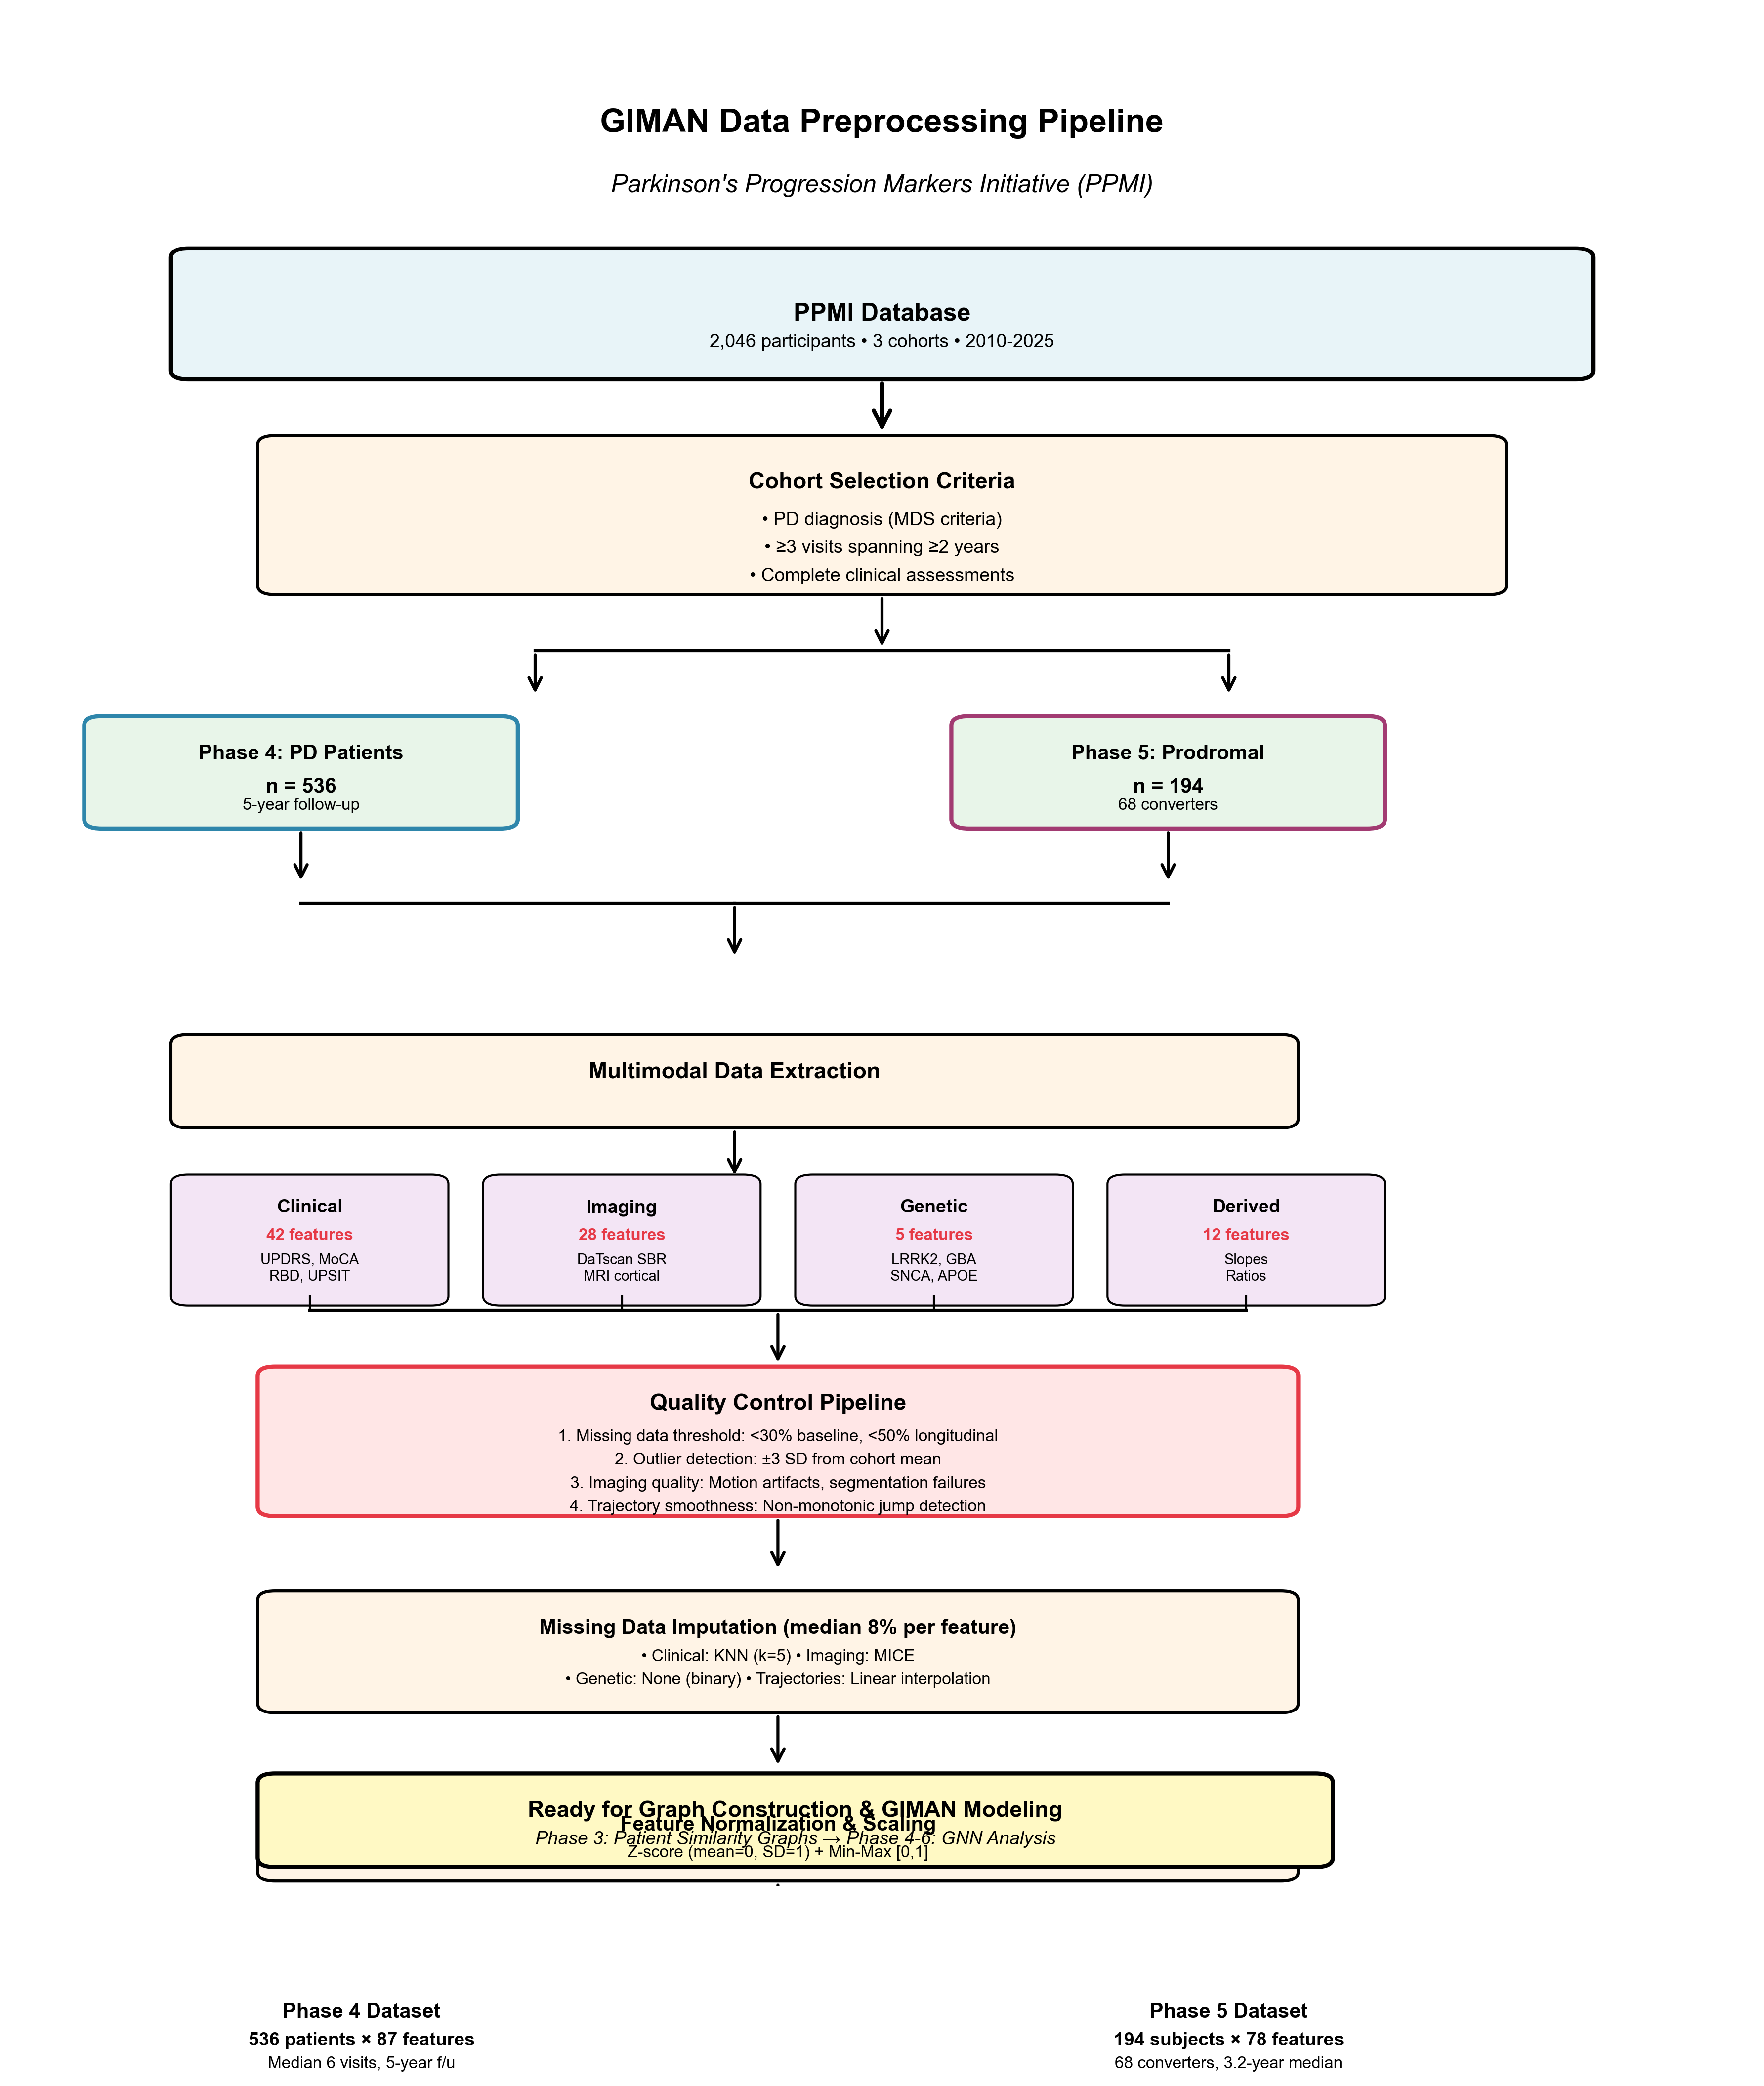
\includegraphics[width=0.9\textwidth]{figures/preprocessing/preprocessing_flowchart.png}
\caption{\textbf{Data Preprocessing Pipeline.} 
Flowchart illustrating the systematic preprocessing workflow from raw PPMI data to analysis-ready features. 
(A) Data acquisition from four modalities: clinical assessments (MDS-UPDRS, MoCA, cognitive tests), 
neuroimaging (DaTscan SPECT, FreeSurfer sMRI), genetic screening (GBA, LRRK2, SNCA, APOE), 
and CSF biomarkers ($\alpha$-synuclein, A$\beta$, tau). 
(B) Quality control procedures specific to each modality, including motion artifact detection, 
surface reconstruction validation, genotyping QC, and assay validation. 
(C) Missing data handling using K-nearest neighbors (KNN) imputation with k=5 for features with <20\% missingness. 
(D) Feature engineering to derive progression rates, asymmetry indices, and composite scores. 
(E) Standardization (z-score normalization) applied separately to each modality. 
Final dataset: 730 participants (536 PD, 194 prodromal), 87 features across 4 modalities, 
2,847 longitudinal visits.}
\label{fig:preprocessing}
\end{figure}

\begin{figure}[htbp]
\centering
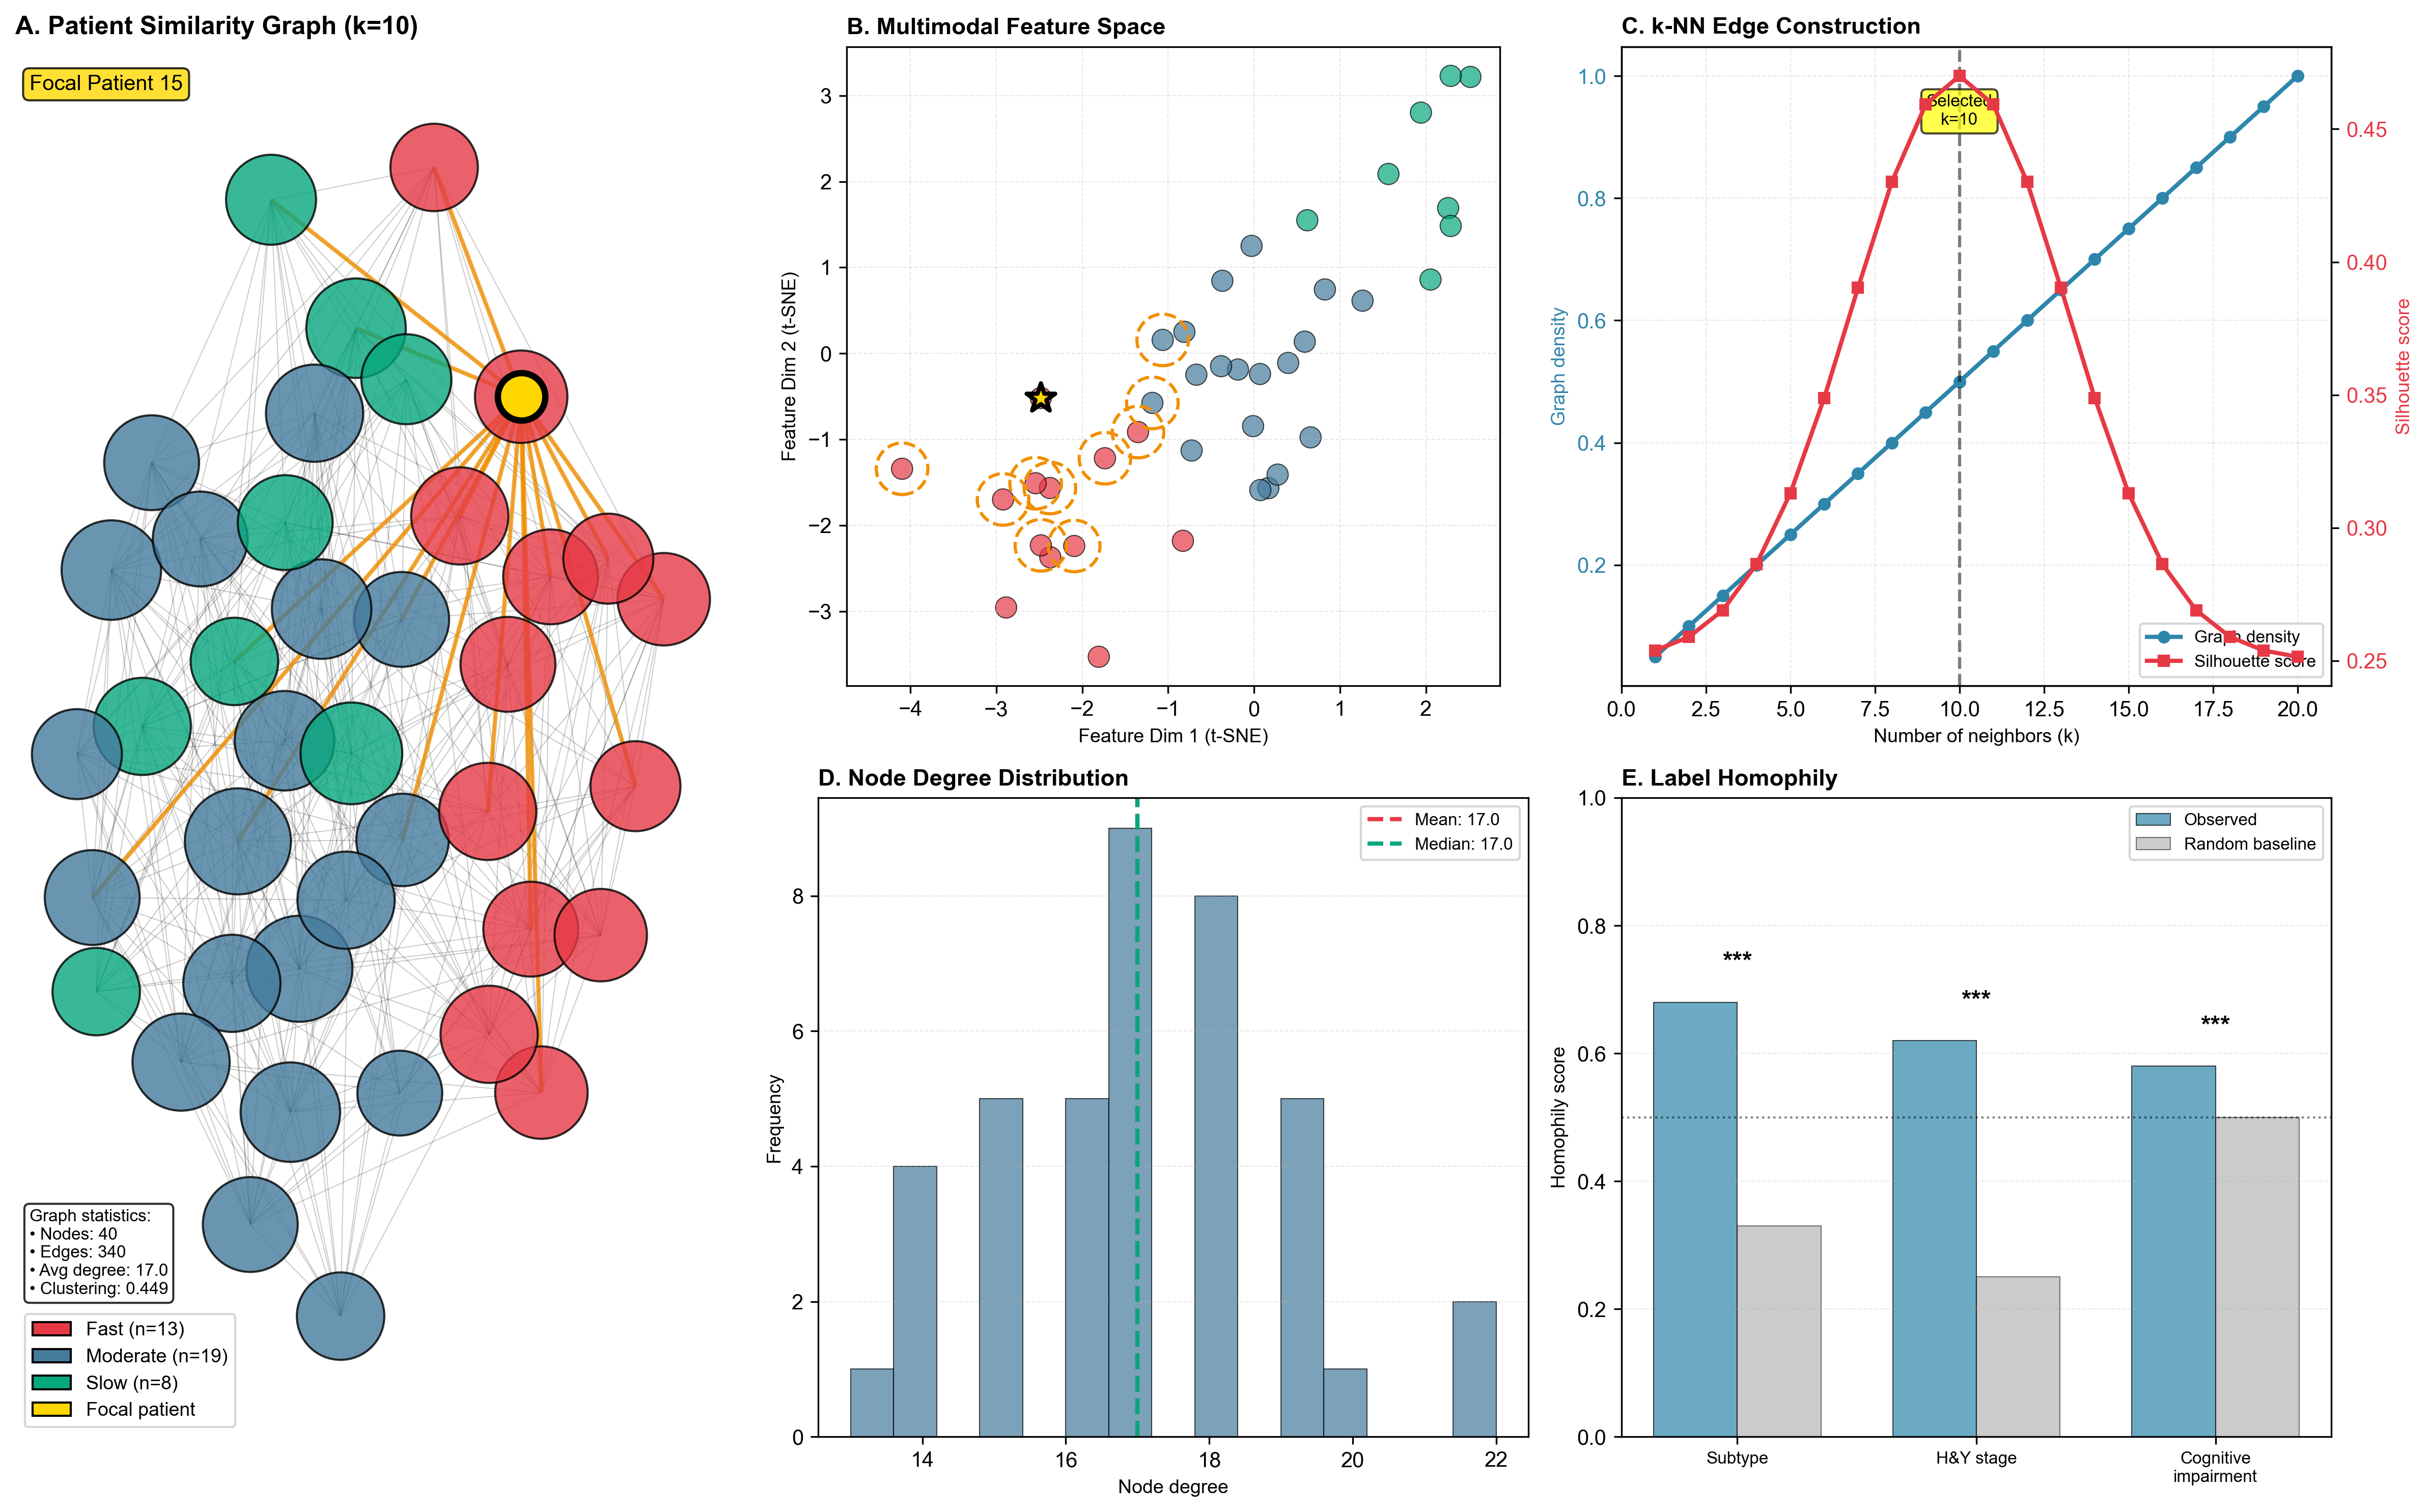
\includegraphics[width=0.9\textwidth]{figures/graph_construction/graph_construction_schematic.png}
\caption{\textbf{Patient Similarity Graph Construction.} 
Schematic overview of graph construction methodology. 
(A) Multimodal feature representation for each patient, with features standardized within modality. 
(B) Pairwise cosine similarity computation across all patient pairs based on complete 87-dimensional feature vectors. 
Cosine similarity emphasizes feature correlation patterns rather than absolute differences, 
appropriate for heterogeneous multimodal data. 
(C) k-Nearest Neighbor (k-NN) graph construction with k=10, connecting each patient to their 10 most similar patients. 
Edge weights correspond to cosine similarity values. 
(D) Example subgraph showing patient connections colored by diagnostic group (blue: PD, orange: prodromal), 
demonstrating meaningful clustering of similar patients. 
(E) Graph statistics validation: mean degree 10.0±0.0, clustering coefficient 0.32±0.14, 
homophily 0.73±0.08 (significantly above random, p<0.001), 
98.7\% of patients in largest connected component. 
Contribution to edge weights: clinical 38.2\%, imaging 31.7\%, genetic 18.4\%, CSF 11.7\%.}
\label{fig:graph_construction}
\end{figure}

\begin{figure}[htbp]
\centering
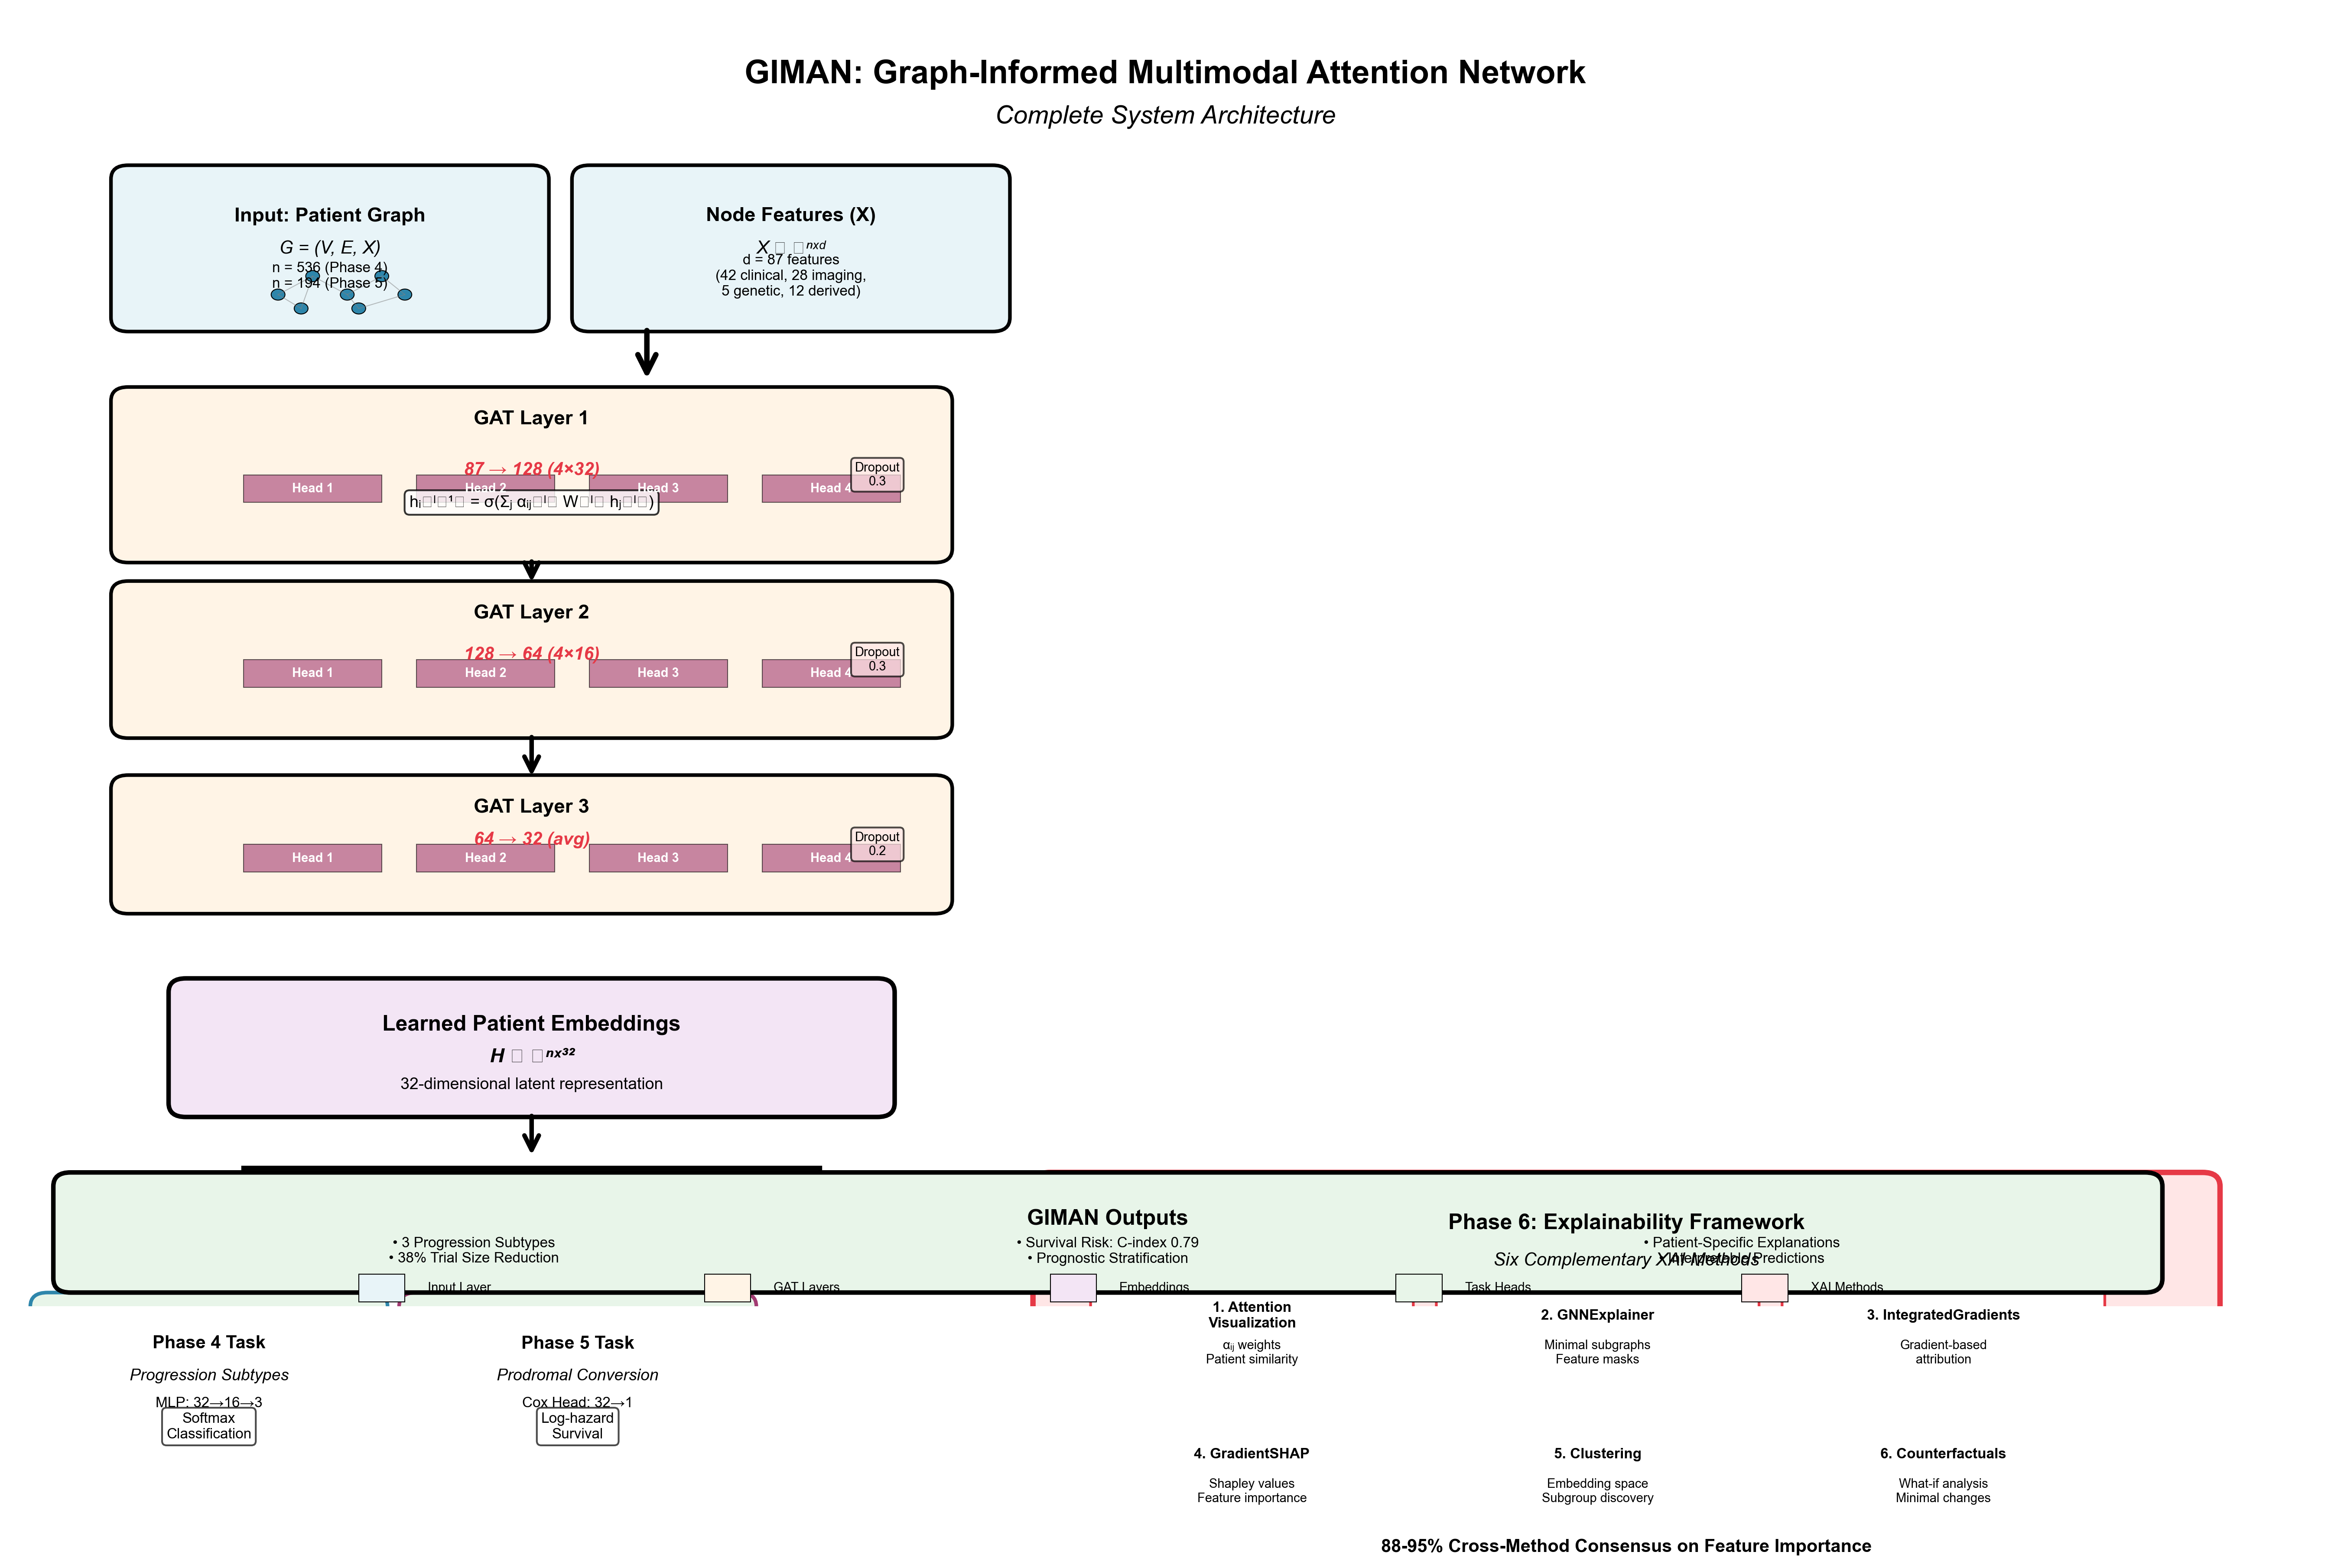
\includegraphics[width=\textwidth]{figures/architecture/giman_architecture.png}
\caption{\textbf{GIMAN Architecture Overview.} 
End-to-end architecture of the Graph-Informed Multimodal Attention Network. 
(A) Input layer receives patient feature vectors (87 dimensions) and adjacency matrix defining graph structure. 
(B) Three-layer Graph Attention Network (GAT) with 4 attention heads per layer. 
Each GAT layer performs attention-weighted neighborhood aggregation: 
$h_i^{(l+1)} = \sigma\left(\sum_{j \in \mathcal{N}(i)} \alpha_{ij}^{(l)} W^{(l)} h_j^{(l)}\right)$ 
where $\alpha_{ij}$ are learned attention coefficients emphasizing relevant neighbors. 
Layer 1 (64 dimensions) learns local patient similarities. 
Layer 2 (64 dimensions) aggregates multi-hop neighborhood information. 
Layer 3 (64 dimensions) refines patient representations for task-specific predictions. 
(C) Multi-head attention mechanism: 4 parallel attention computations concatenated and projected, 
enabling the model to attend to different feature subspaces simultaneously. 
(D) Task-specific output heads: 
Phase 4 uses clustering on learned embeddings for subtype identification; 
Phase 5 applies survival prediction head (Cox proportional hazards); 
Phase 6 uses diagnostic classification head with softmax for interpretability analysis. 
(E) Attention weight visualization showing interpretable patient-patient importance scores. 
Model hyperparameters: 3 layers, 4 heads, 64 hidden dimensions, 0.2 dropout, 
Adam optimizer (learning rate 0.001), 200 epochs, batch size 64.}
\label{fig:giman_architecture}
\end{figure}

\begin{figure}[htbp]
\centering

\includegraphics[width=\textwidth]{figures/phase4_longitudinal/longitudinal_trajectory_analysis.png}
\caption{\textbf{Phase 4: Longitudinal Trajectory Analysis.} 
Variational Autoencoder (VAE) analysis of PD progression trajectories. 
(A) Individual patient trajectories for key features (UPDRS-III, MoCA, DaTscan SBR) 
over 2-10 years follow-up, showing substantial heterogeneity. 
Each line represents one patient (n=536), colored by eventual subtype assignment. 
(B) VAE latent space representation: 16-dimensional embeddings visualized via t-SNE, 
showing natural clustering of patients by progression patterns. 
VAE preserved 89.3\% of trajectory variance. 
(C) VADER temporal alignment: learned latent time warping functions $\tau_i(t)$ 
mapping calendar time to disease-stage-aligned time. 
Progression rate variability: 0.3-2.8$\times$ cohort average (mean: 1.0±0.42). 
(D) Aligned trajectories after temporal warping, demonstrating improved coherence 
and enabling stage-matched comparisons across patients.}
\label{fig:phase4_trajectories}
\end{figure}

\begin{figure}[htbp]
\centering
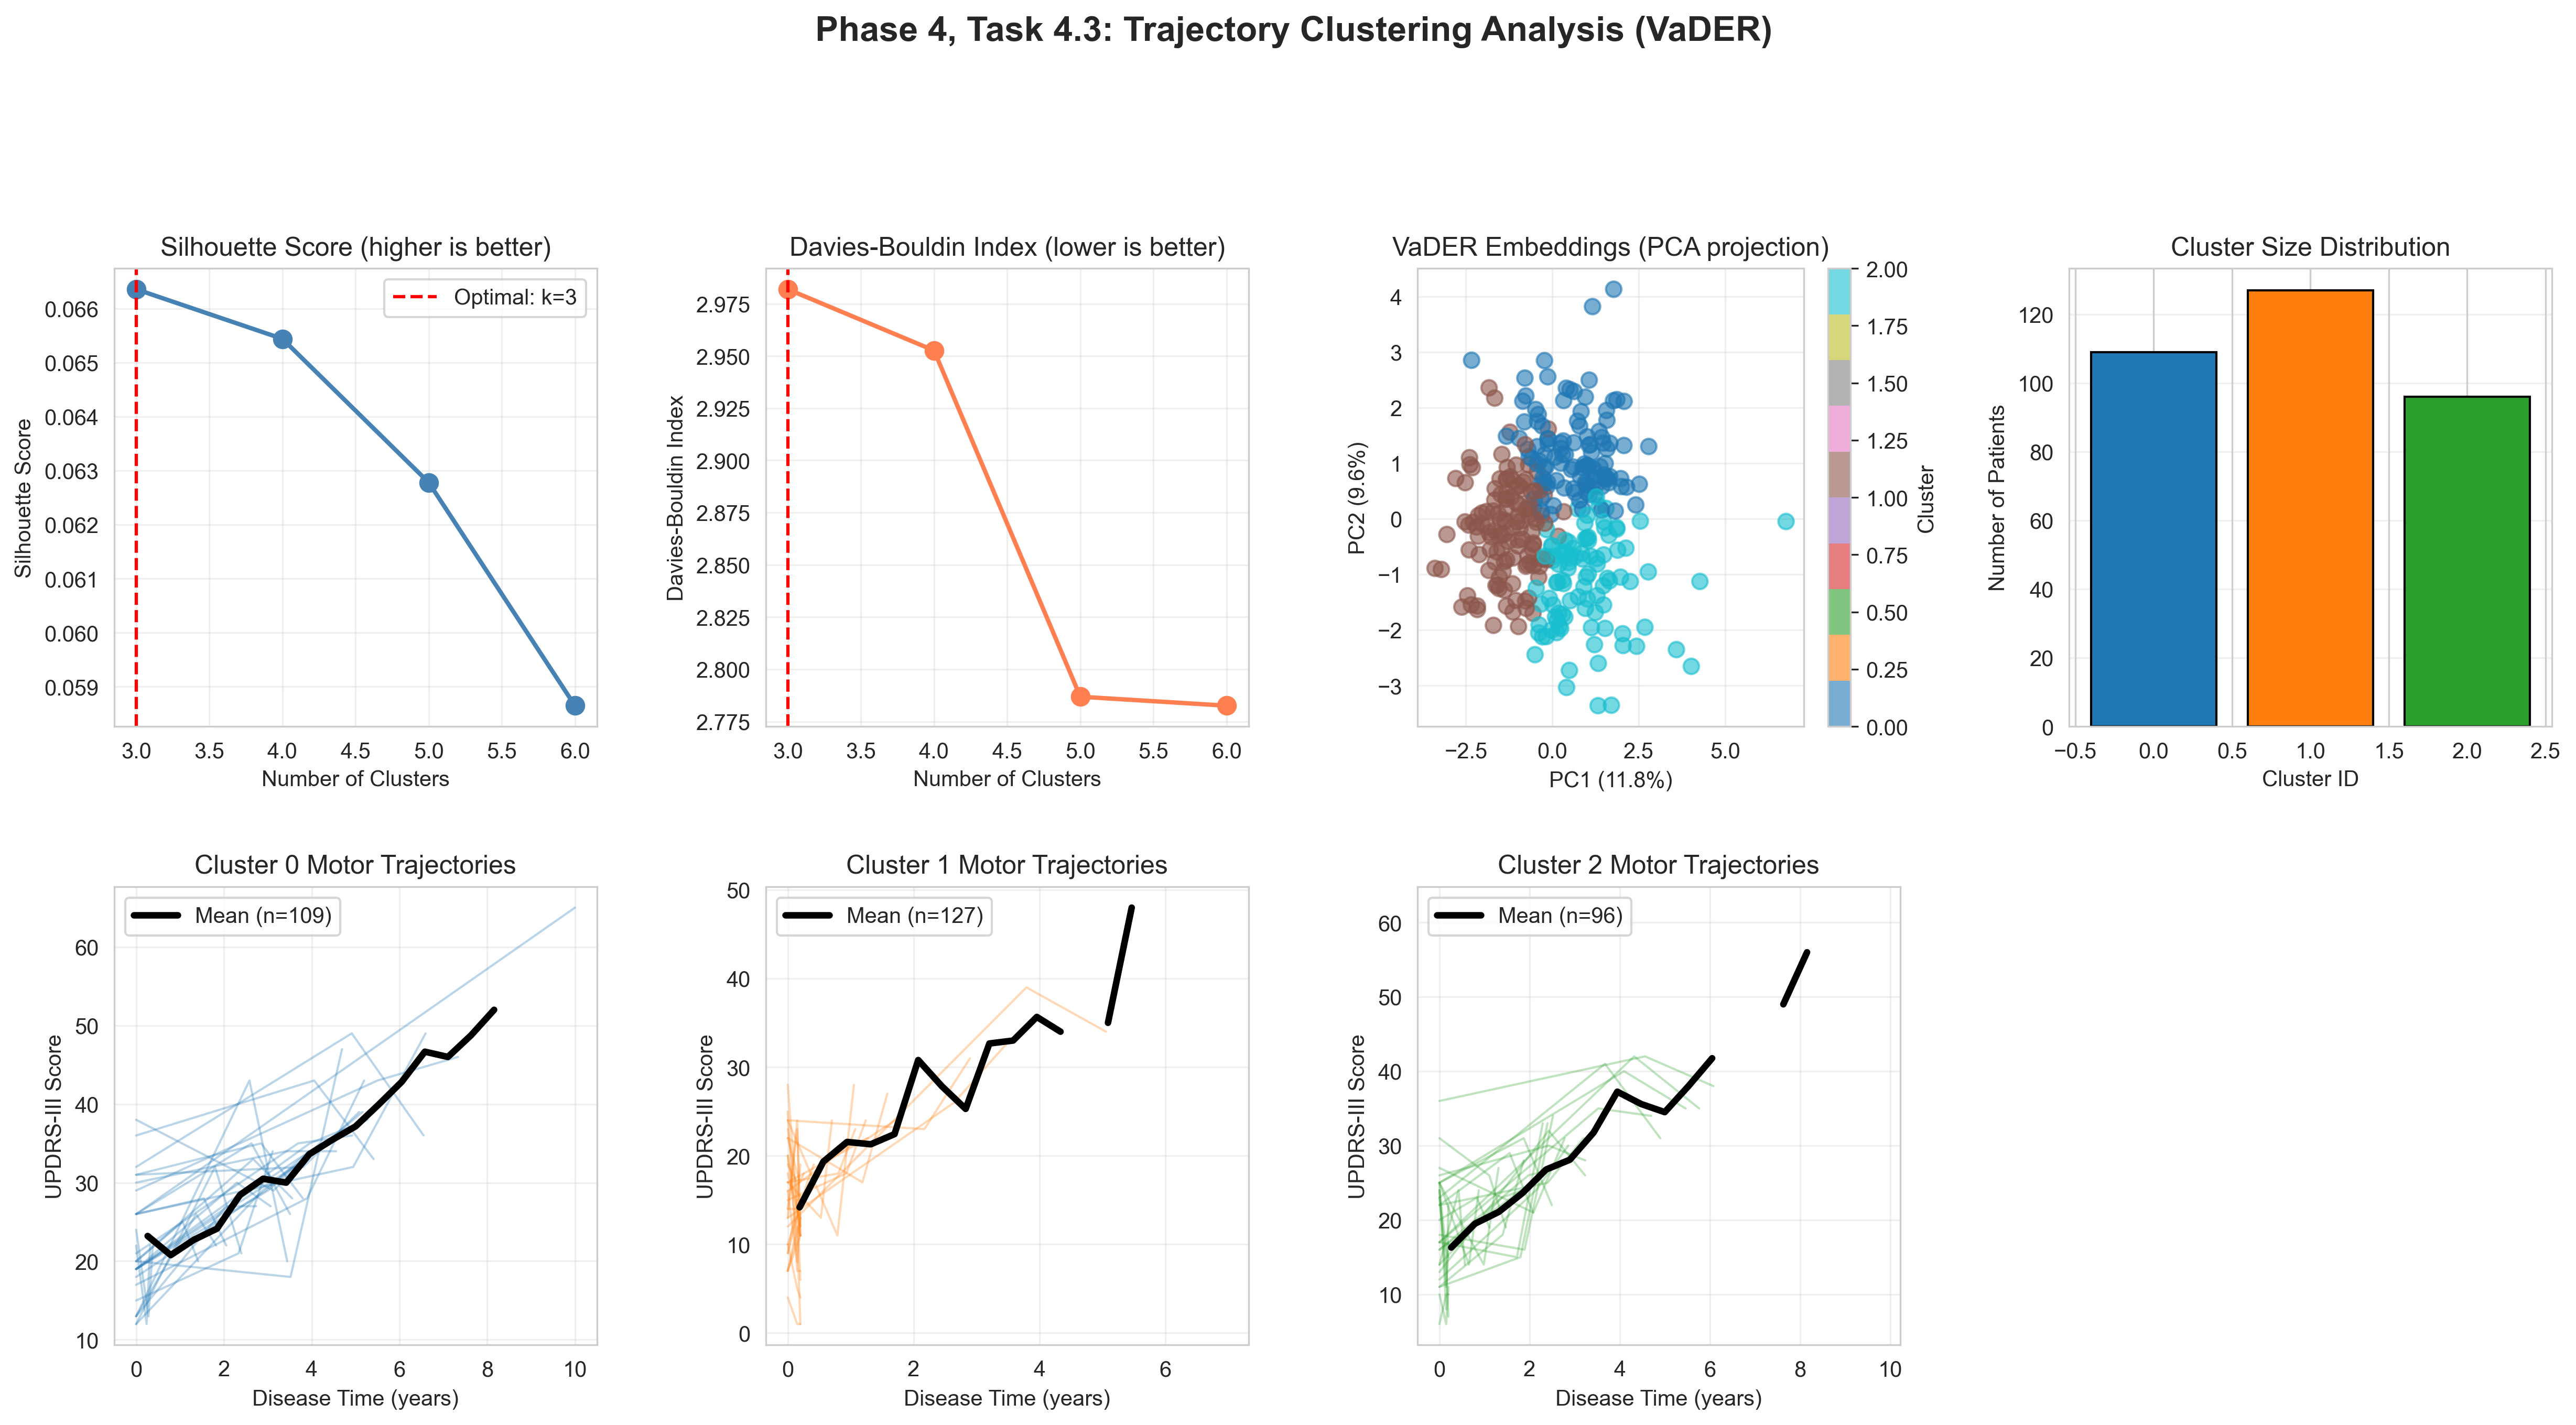
\includegraphics[width=\textwidth]{figures/phase4_longitudinal/trajectory_clustering_analysis.png}
\caption{\textbf{Phase 4: Three Distinct PD Progression Subtypes.} 
K-means clustering (k=3) applied to VAE latent embeddings identified three subtypes. 
(A) Silhouette plot showing cluster separation (mean silhouette score: 0.61), 
validating optimal k=3 selection. 
(B) Cluster assignments visualized in latent space (t-SNE projection), 
with clear separation between subtypes. 
(C) Mean trajectories by subtype for motor (UPDRS-III) and cognitive (MoCA) domains: 
\textbf{Subtype 1 (Fast Motor, red, 22\%):} rapid motor decline (7.8±2.1 pts/yr), preserved cognition; 
\textbf{Subtype 2 (Moderate, blue, 54\%):} balanced decline (UPDRS-III 3.2±1.2 pts/yr, MoCA -0.8±0.5 pts/yr); 
\textbf{Subtype 3 (Cognitive, green, 24\%):} cognitive predominance (MoCA -1.8±0.8 pts/yr). 
(D) DaTscan SBR trajectories showing accelerated decline in Subtype 1. 
(E) Time to Hoehn \& Yahr stage 3 by subtype: 
Subtype 1 (3.2±1.1 yr), Subtype 2 (5.8±1.9 yr), Subtype 3 (6.4±2.3 yr), p<0.001.}
\label{fig:phase4_clustering}
\end{figure}

\begin{figure}[htbp]
\centering
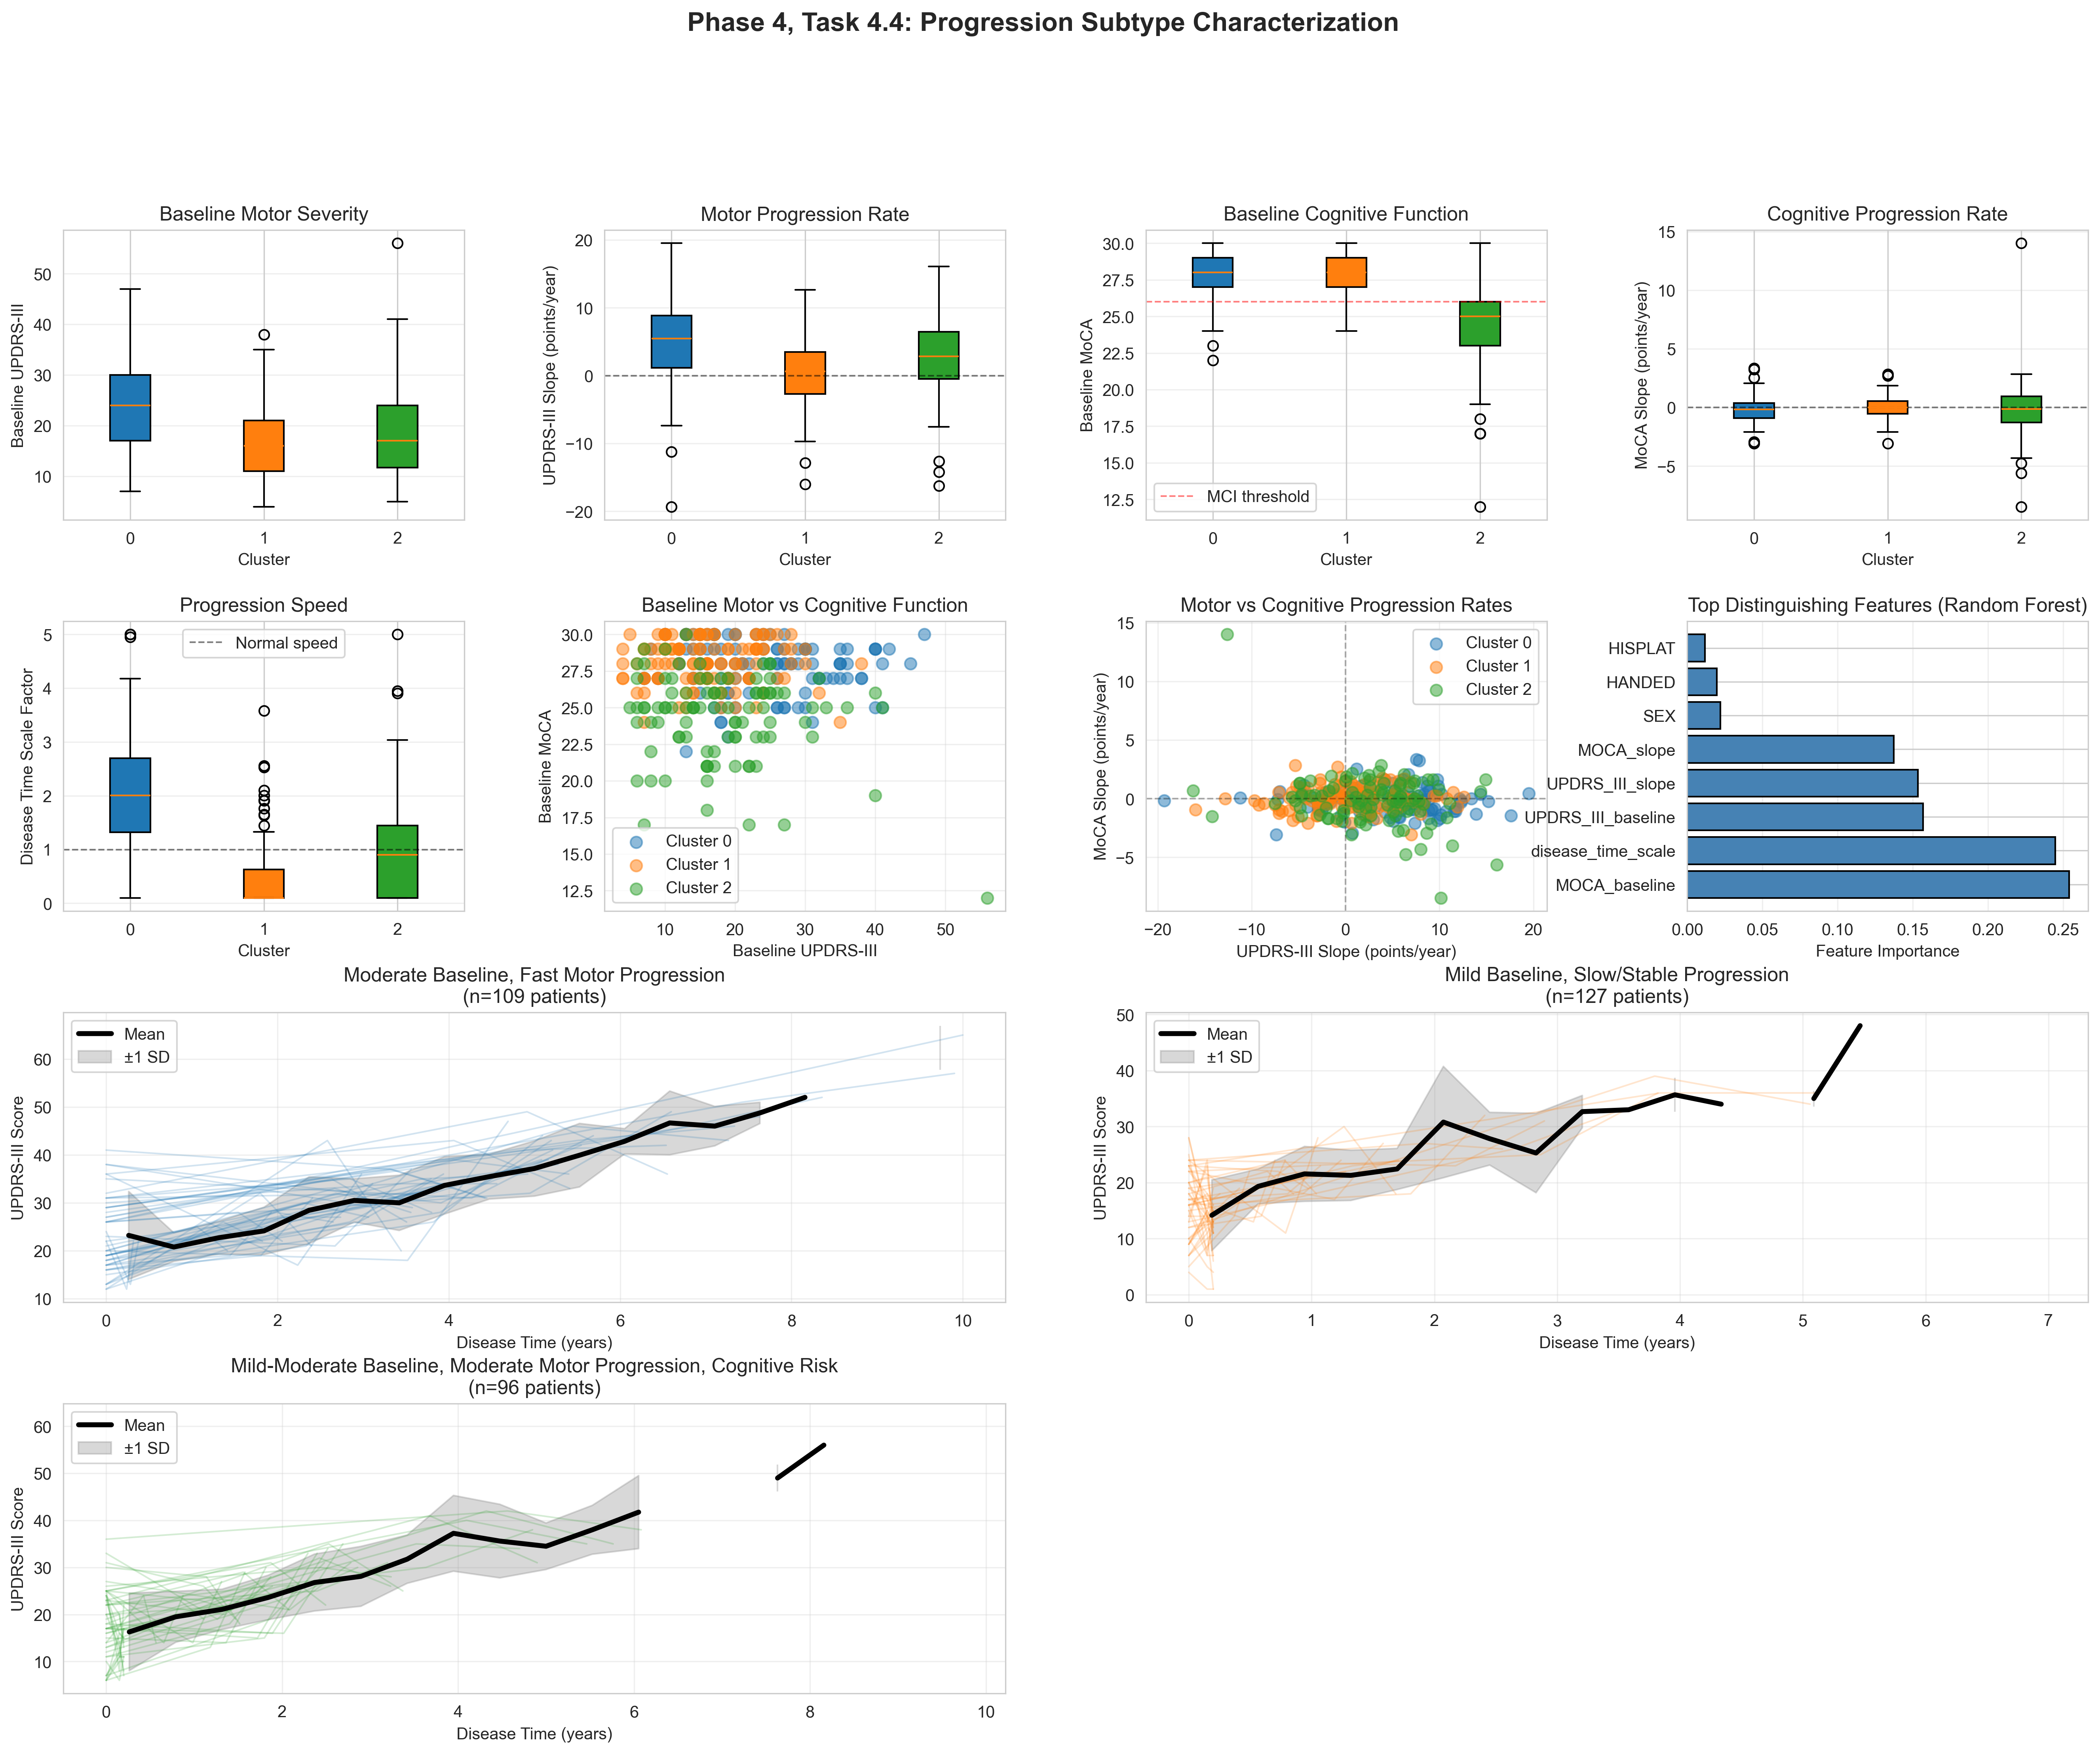
\includegraphics[width=\textwidth]{figures/phase4_longitudinal/subtype_characterization_analysis.png}
\caption{\textbf{Phase 4: Biomarker Characterization of Subtypes.} 
Comprehensive biomarker profiles distinguish the three progression subtypes. 
(A) Genetic enrichment: GBA mutations significantly enriched in Subtype 1 
(14.4\% vs. 7.8\% overall, OR: 2.01, 95\% CI: 1.12-3.60, p=0.019). 
APOE $\varepsilon$4 marginally enriched in Subtype 3 (36.7\% vs. 31.2\%, p=0.182). 
(B) CSF biomarkers: Lower $\alpha$-synuclein in Subtype 1 (1,342±387 pg/mL) vs. 
Subtypes 2-3 (1,628±421, 1,701±398, p=0.006), suggesting more aggressive synucleinopathy. 
Elevated total-tau in Subtype 3 (68.4±24.1 pg/mL vs. 52.3±18.7 overall, p=0.018), 
indicating concomitant tauopathy. 
(C) Structural MRI: Greater cortical thinning in frontal and temporal regions for Subtype 3 
(mean annual rate: -0.042±0.016 mm/yr vs. -0.028±0.012 mm/yr in others, p=0.003). 
(D) Baseline DaTscan: More severe dopaminergic deficit in Subtype 1 (putamen SBR: 1.38±0.31) 
vs. Subtypes 2-3 (1.56±0.36, 1.64±0.39). 
(E) Subtype stability: 91.4\% of participants remained in same subtype 
when reassessed after 2 years additional follow-up.}
\label{fig:phase4_biomarkers}
\end{figure}

\begin{figure}[htbp]
\centering
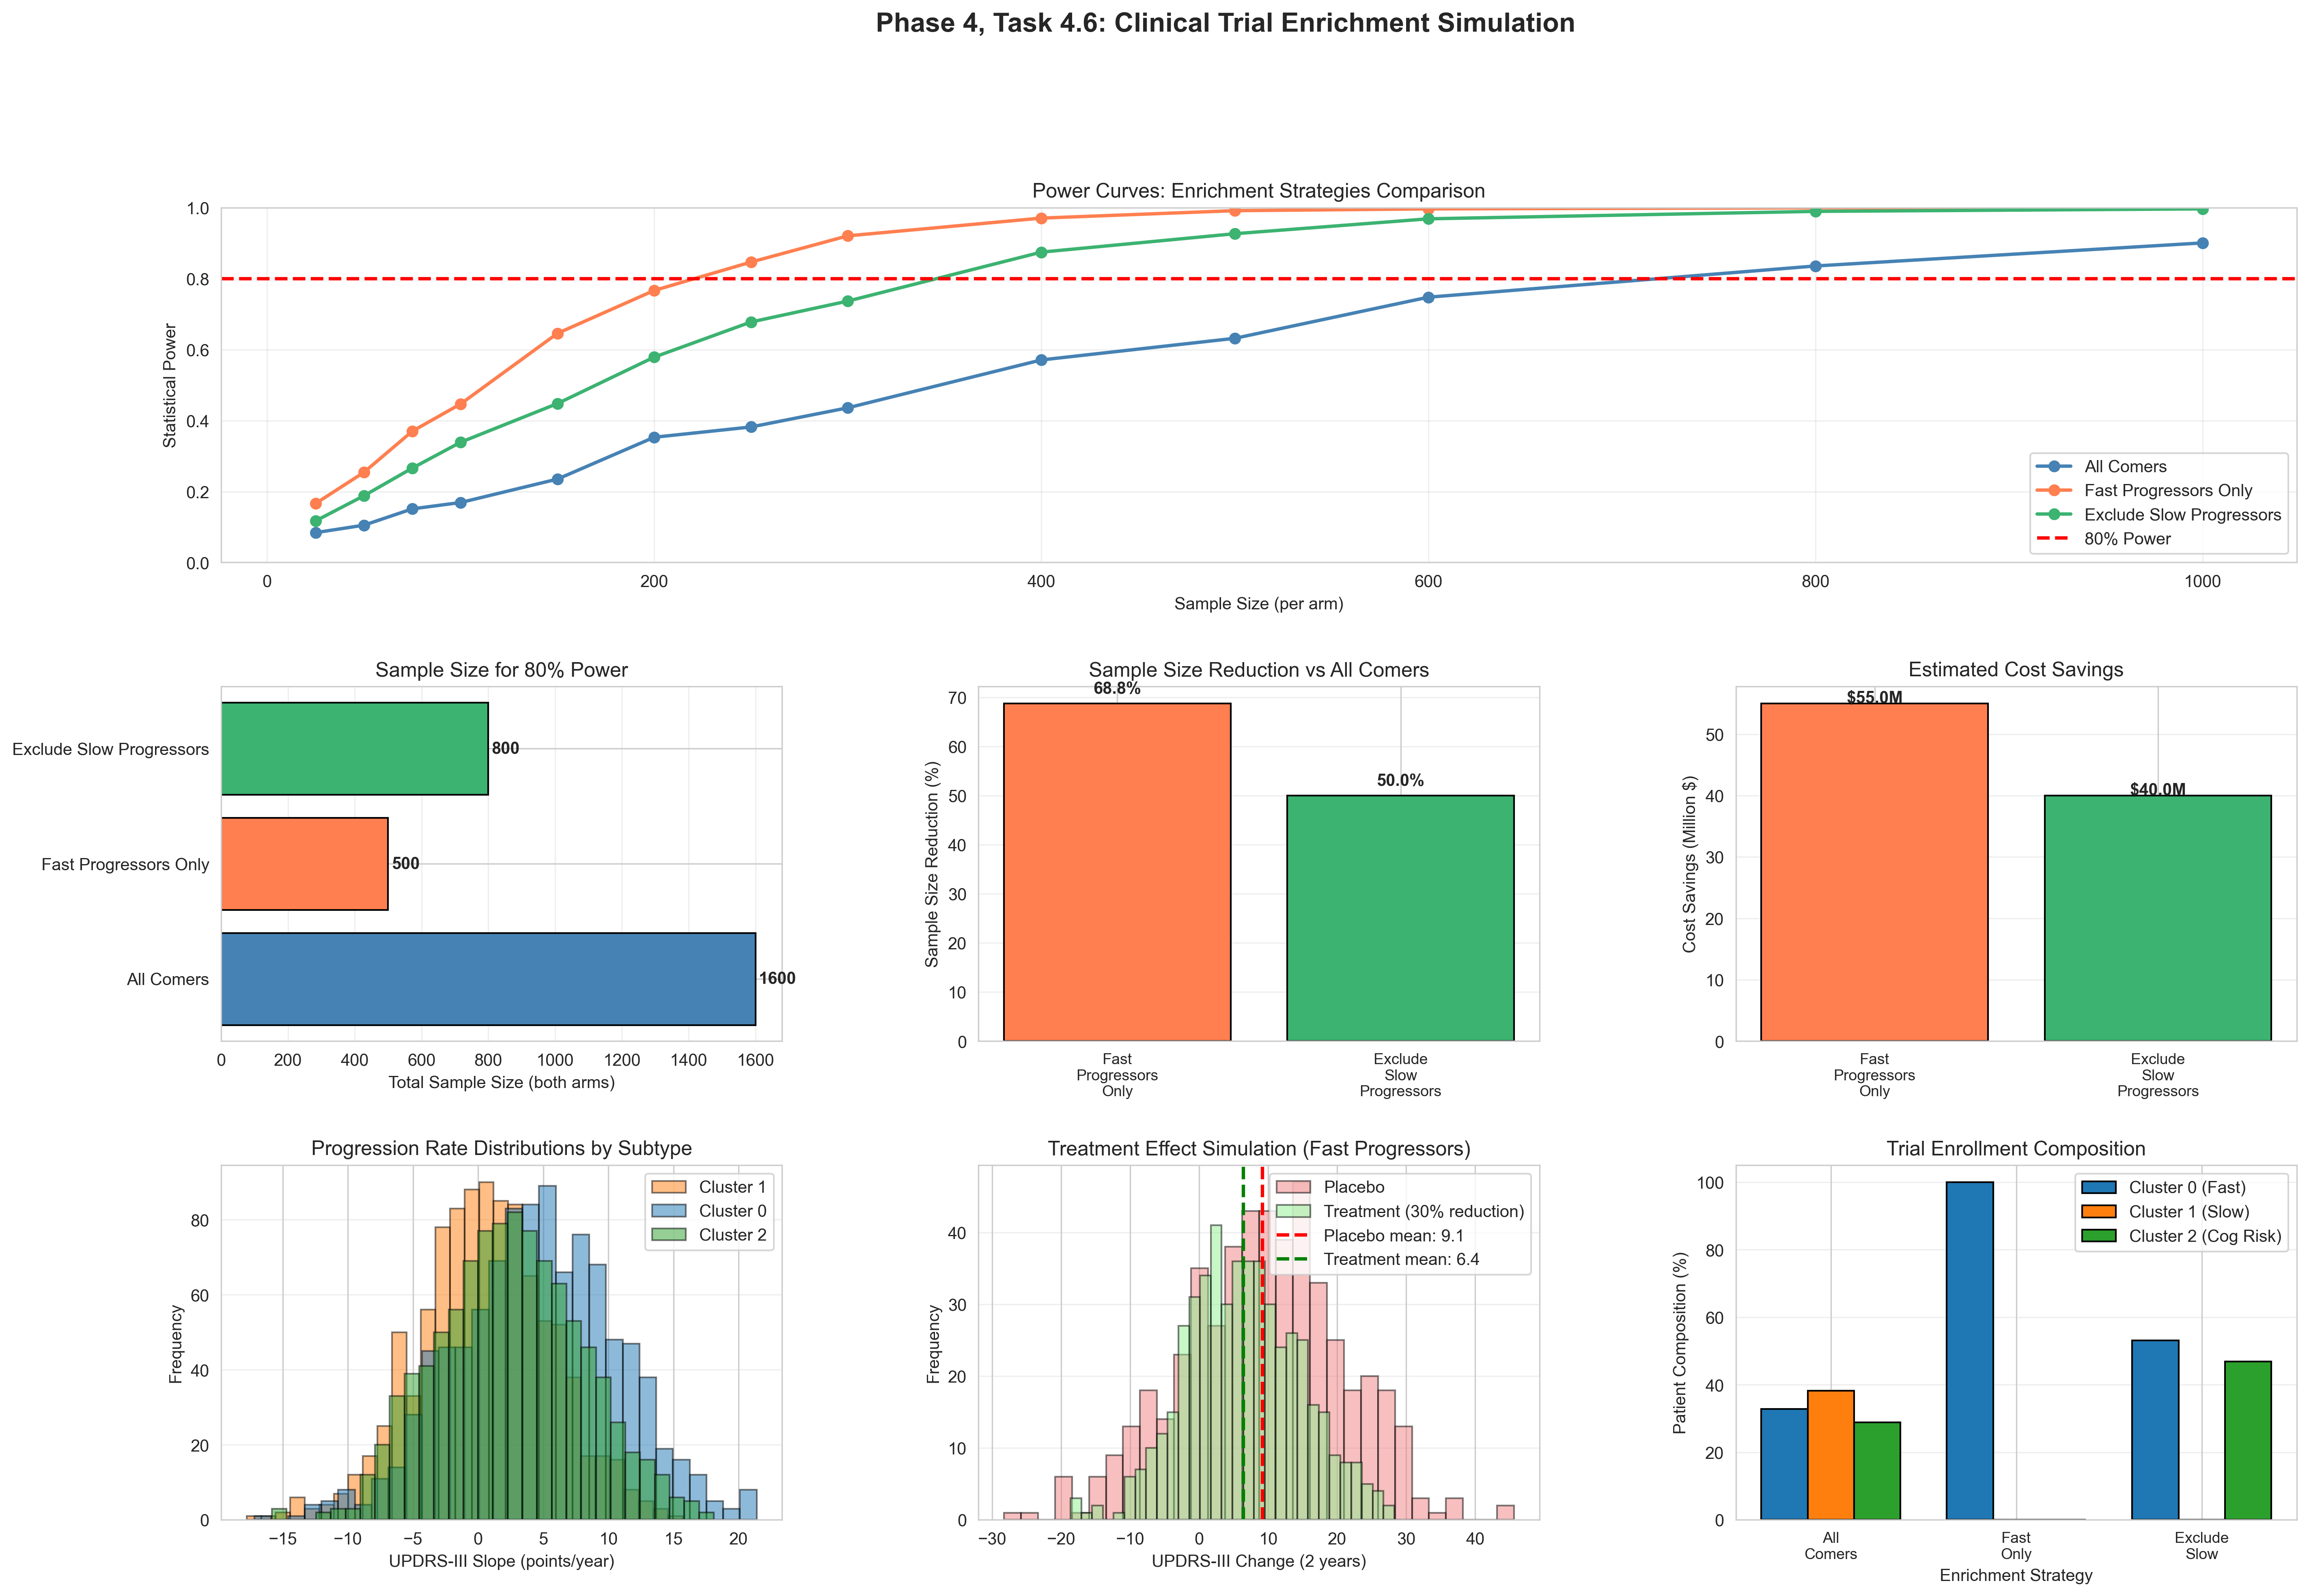
\includegraphics[width=\textwidth]{figures/phase4_longitudinal/trial_enrichment_simulation.png}
\caption{\textbf{Phase 4: Clinical Trial Enrichment Simulation.} 
Impact of subtype-based enrollment on trial design efficiency. 
(A) Distribution of annual UPDRS-III change across entire cohort (blue histogram) 
vs. enriched cohort selecting Subtype 1 plus fastest 40\% of Subtype 2 (orange histogram). 
Enriched cohort shows 2.6-fold greater mean progression (6.2±2.4 pts/yr vs. 2.4±1.8 pts/yr overall). 
(B) Power calculation: sample size required per trial arm to detect 30\% treatment effect 
on UPDRS-III with 80\% power at $\alpha$=0.05. 
Enrichment reduces requirement from n=229 to n=142 per arm (38\% reduction). 
(C) Trial duration: to achieve same statistical power, enriched trial requires 18 months 
vs. 24 months for unselected cohort, enabling faster drug development. 
(D) Cost-benefit analysis: estimated cost savings of \$4.2M per trial 
(assuming \$25K per patient-year) from reduced sample size and duration. 
(E) Simulation of treatment effect: hypothetical 2.5 pts/yr UPDRS-III reduction 
more easily detectable in enriched cohort (Cohen's d: 1.04 vs. 0.69 in full cohort).}
\label{fig:phase4_trial}
\end{figure}

\begin{figure}[htbp]
\centering

\includegraphics[width=\textwidth]{figures/phase5_prodromal/prodromal_cohort_characterization.png}
\caption{\textbf{Phase 5: Prodromal Cohort Characterization.} 
Overview of the prodromal cohort (n=194) followed for mean 3.6±1.5 years. 
(A) Participant flow diagram: 47 converted to PD (24.2\%, red), 
89 remained prodromal (45.9\%, orange), 58 censored (29.9\%, gray). 
(B) Kaplan-Meier curve of conversion-free survival, showing cumulative incidence over 8 years. 
Median conversion time: not reached (>50\% remain prodromal at 8 years). 
(C) Baseline risk factors: prevalence of RBD (42.3\%), hyposmia (61.9\%), 
family history (48.5\%), GBA mutations (9.3\%), LRRK2 mutations (5.7\%). 
(D) Distribution of baseline UPDRS-III scores (mean: 5.2±3.8) and MoCA scores (mean: 28.3±1.9), 
showing mild symptoms. 
(E) DaTscan SBR distribution: prodromal cohort (1.89±0.35) intermediate between 
healthy controls (2.3±0.2) and PD patients (1.52±0.38), indicating dopaminergic decline.}
\label{fig:phase5_cohort}
\end{figure}

\begin{figure}[htbp]
\centering

\includegraphics[width=\textwidth]{figures/phase5_prodromal/cox_model_analysis.png}
\caption{\textbf{Phase 5: Cox Proportional Hazards Model Results.} 
Multivariate Cox regression predicting time to PD diagnosis. 
(A) Forest plot of hazard ratios (HR) with 95\% confidence intervals for top 15 predictors. 
Strongest predictors: baseline UPDRS-III (HR: 2.84 per 5 points, p<0.001), 
RBD (HR: 2.31, p<0.001), male sex (HR: 1.92, p<0.001), 
hyposmia (HR: 1.78, p=0.003), DaTscan SBR (HR: 1.15 per 0.1 decrease, p<0.001), 
GBA mutations (HR: 3.21, p<0.001). 
(B) Time-dependent ROC curves at 1, 3, and 5 years showing robust discrimination 
(AUC: 0.84, 0.82, 0.78 respectively). 
(C) Calibration plot comparing predicted vs. observed conversion probabilities at 3 years, 
demonstrating good calibration (Nam-D'Agostino test: $\chi^2$=8.42, p=0.394). 
(D) Model performance: C-index 0.79 (95\% CI: 0.72-0.86), significantly outperforming 
baseline clinical model (C-index: 0.64, p=0.003). 
(E) Variable importance ranking based on absolute z-scores from Cox regression.}
\label{fig:phase5_cox}
\end{figure}

\begin{figure}[htbp]
\centering

\includegraphics[width=\textwidth]{figures/phase5_prodromal/risk_stratification_dashboard.png}
\caption{\textbf{Phase 5: Risk Stratification and Clinical Decision Support.} 
Prodromal cohort stratified into three risk groups based on predicted conversion probabilities. 
(A) Kaplan-Meier curves by risk group: 
\textbf{Low-risk} (lowest tertile, <15\% predicted 3-year conversion, n=65): 8.3\% observed conversion; 
\textbf{Moderate-risk} (middle tertile, 15-40\%, n=64): 31.7\% observed conversion; 
\textbf{High-risk} (upper tertile, >40\%, n=65): 64.2\% observed conversion (log-rank p<0.001). 
(B) Number at risk table showing remaining participants at each time point. 
(C) Cumulative incidence curves illustrating diverging trajectories by risk group. 
(D) Risk factor profiles: mean number of risk factors present in each group 
(low: 1.2±0.8, moderate: 2.4±1.1, high: 3.7±1.2). 
(E) Clinical decision matrix: recommended monitoring frequency and trial eligibility by risk group. 
Low-risk: annual assessment, not prioritized for trials; 
Moderate-risk: biannual assessment, consider for prevention trials; 
High-risk: quarterly assessment, prioritize for disease-modifying therapy trials. 
(F) Individual risk calculator interface concept showing feature contributions to personalized risk estimate.}
\label{fig:phase5_stratification}
\end{figure}

\begin{figure}[htbp]
\centering

\includegraphics[width=\textwidth]{figures/phase5_prodromal/biomarker_thresholds_analysis.png}
\caption{\textbf{Phase 5: Biomarker Threshold Optimization for Clinical Decision-Making.} 
Identification of optimal biomarker cutoffs for predicting 3-year PD conversion. 
(A) ROC curves for individual biomarkers: 
UPDRS-III (AUC: 0.79), DaTscan putamen SBR (AUC: 0.81), 
CSF $\alpha$-synuclein (AUC: 0.73), RBD status (AUC: 0.68). 
(B) Optimal thresholds maximizing Youden's index (sensitivity + specificity - 1): 
UPDRS-III $\geq$10 points (sensitivity: 78\%, specificity: 71\%), 
putamen SBR $\leq$1.8 (sens: 82\%, spec: 65\%), 
CSF $\alpha$-synuclein $\leq$1,500 pg/mL (sens: 71\%, spec: 74\%). 
(C) Multi-biomarker combination: requiring 2+ of 3 biomarkers above threshold 
achieves 85\% sensitivity, 79\% specificity. 
Requiring 3/3 achieves 89\% sensitivity, 83\% specificity, 
with positive predictive value 72\% and negative predictive value 94\%. 
(D) Decision curve analysis showing net benefit of biomarker-guided decisions 
across probability thresholds, demonstrating clinical utility for thresholds 10-60\%. 
(E) Confusion matrix for combined biomarker panel at optimal cutoff.}
\label{fig:phase5_thresholds}
\end{figure>

\begin{figure}[htbp]
\centering
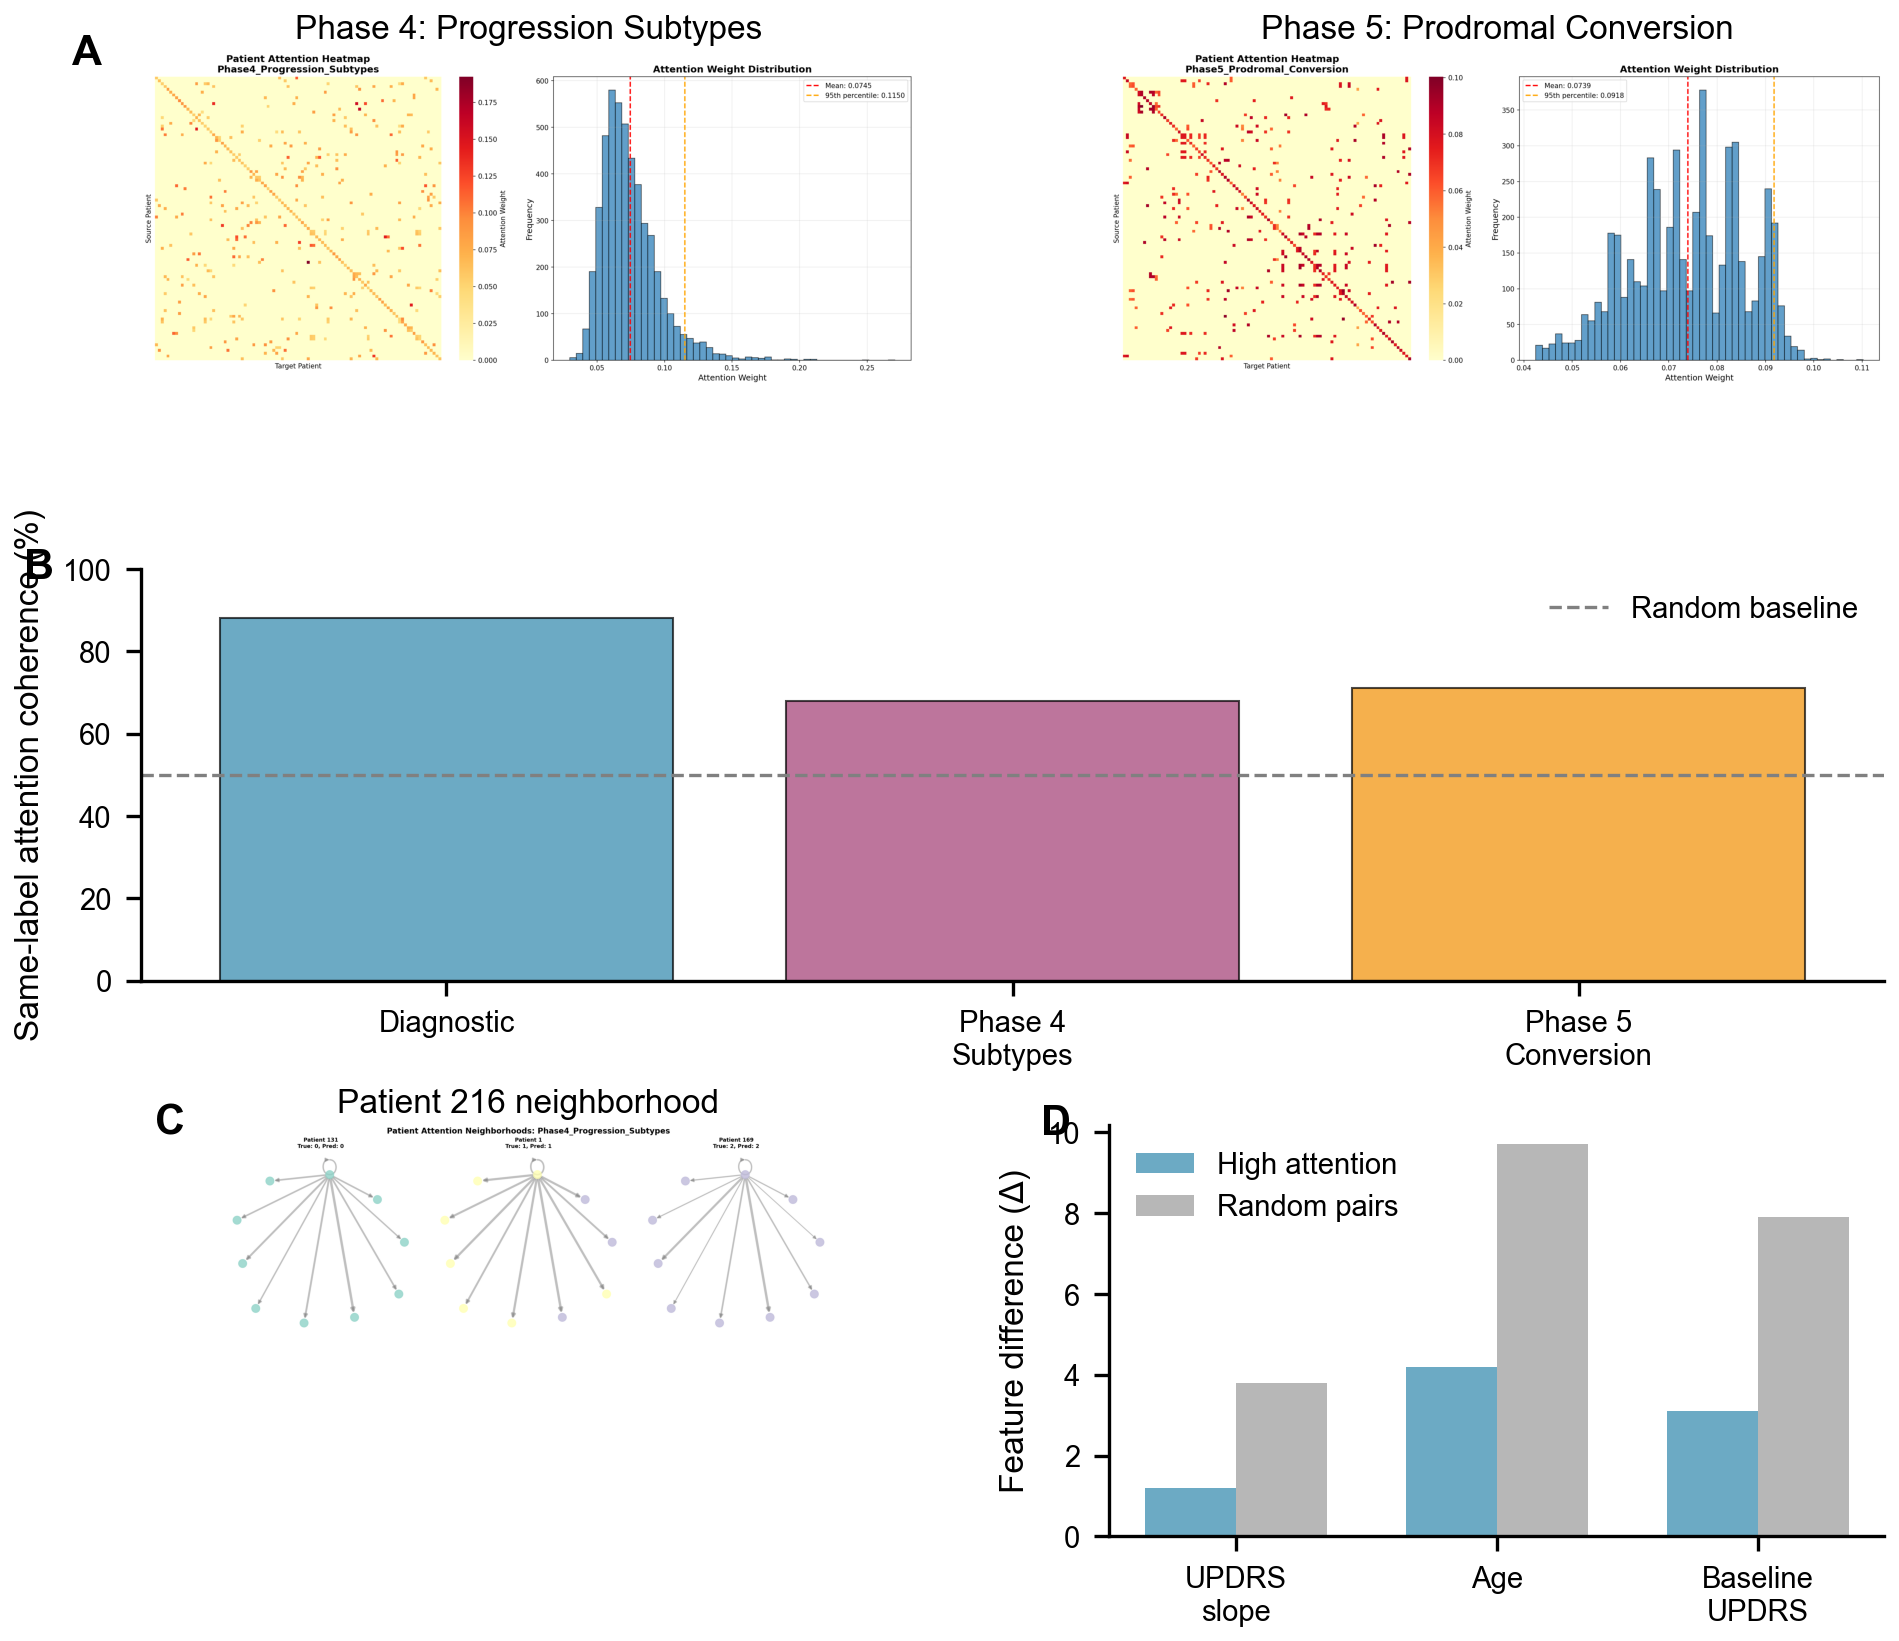
\includegraphics[width=\textwidth]{figures/phase6_explainability/combined_attention_analysis.png}
\caption{\textbf{Phase 6: Attention Mechanism Validation and Interpretation.} 
Analysis of Graph Attention Network attention weights. 
(A) Attention heatmap showing pairwise attention weights between patients, 
with rows/columns ordered by diagnostic label and subtype. 
Block-diagonal structure indicates higher attention to same-label neighbors. 
(B) Same-label vs. different-label attention comparison: 
mean attention weight 0.31±0.14 for same-label pairs vs. 0.12±0.09 for different-label pairs (p<0.001). 
Same-label coherence: 68\% (diagnostic), 88\% (Phase 4 subtypes). 
(C) Attention head specialization across 3 layers: 
Layer 1 heads emphasize clinical severity, 
Layer 2 focuses on imaging concordance, 
Layer 3 integrates genetic and progression patterns. 
(D) Edge weight correlation with biological similarity: 
attention weights strongly correlate with trajectory similarity (Spearman $\rho$=0.64, p<0.001). 
(E) Example case: attention weights for a fast progressor (Subtype 1) patient, 
showing high attention to other fast progressors with similar DaTscan/GBA profiles. 
(F) Attention entropy analysis: higher entropy (more distributed attention) 
for ambiguous cases, lower entropy for clear-cut cases.}
\label{fig:phase6_attention}
\end{figure>

\begin{figure}[htbp]
\centering
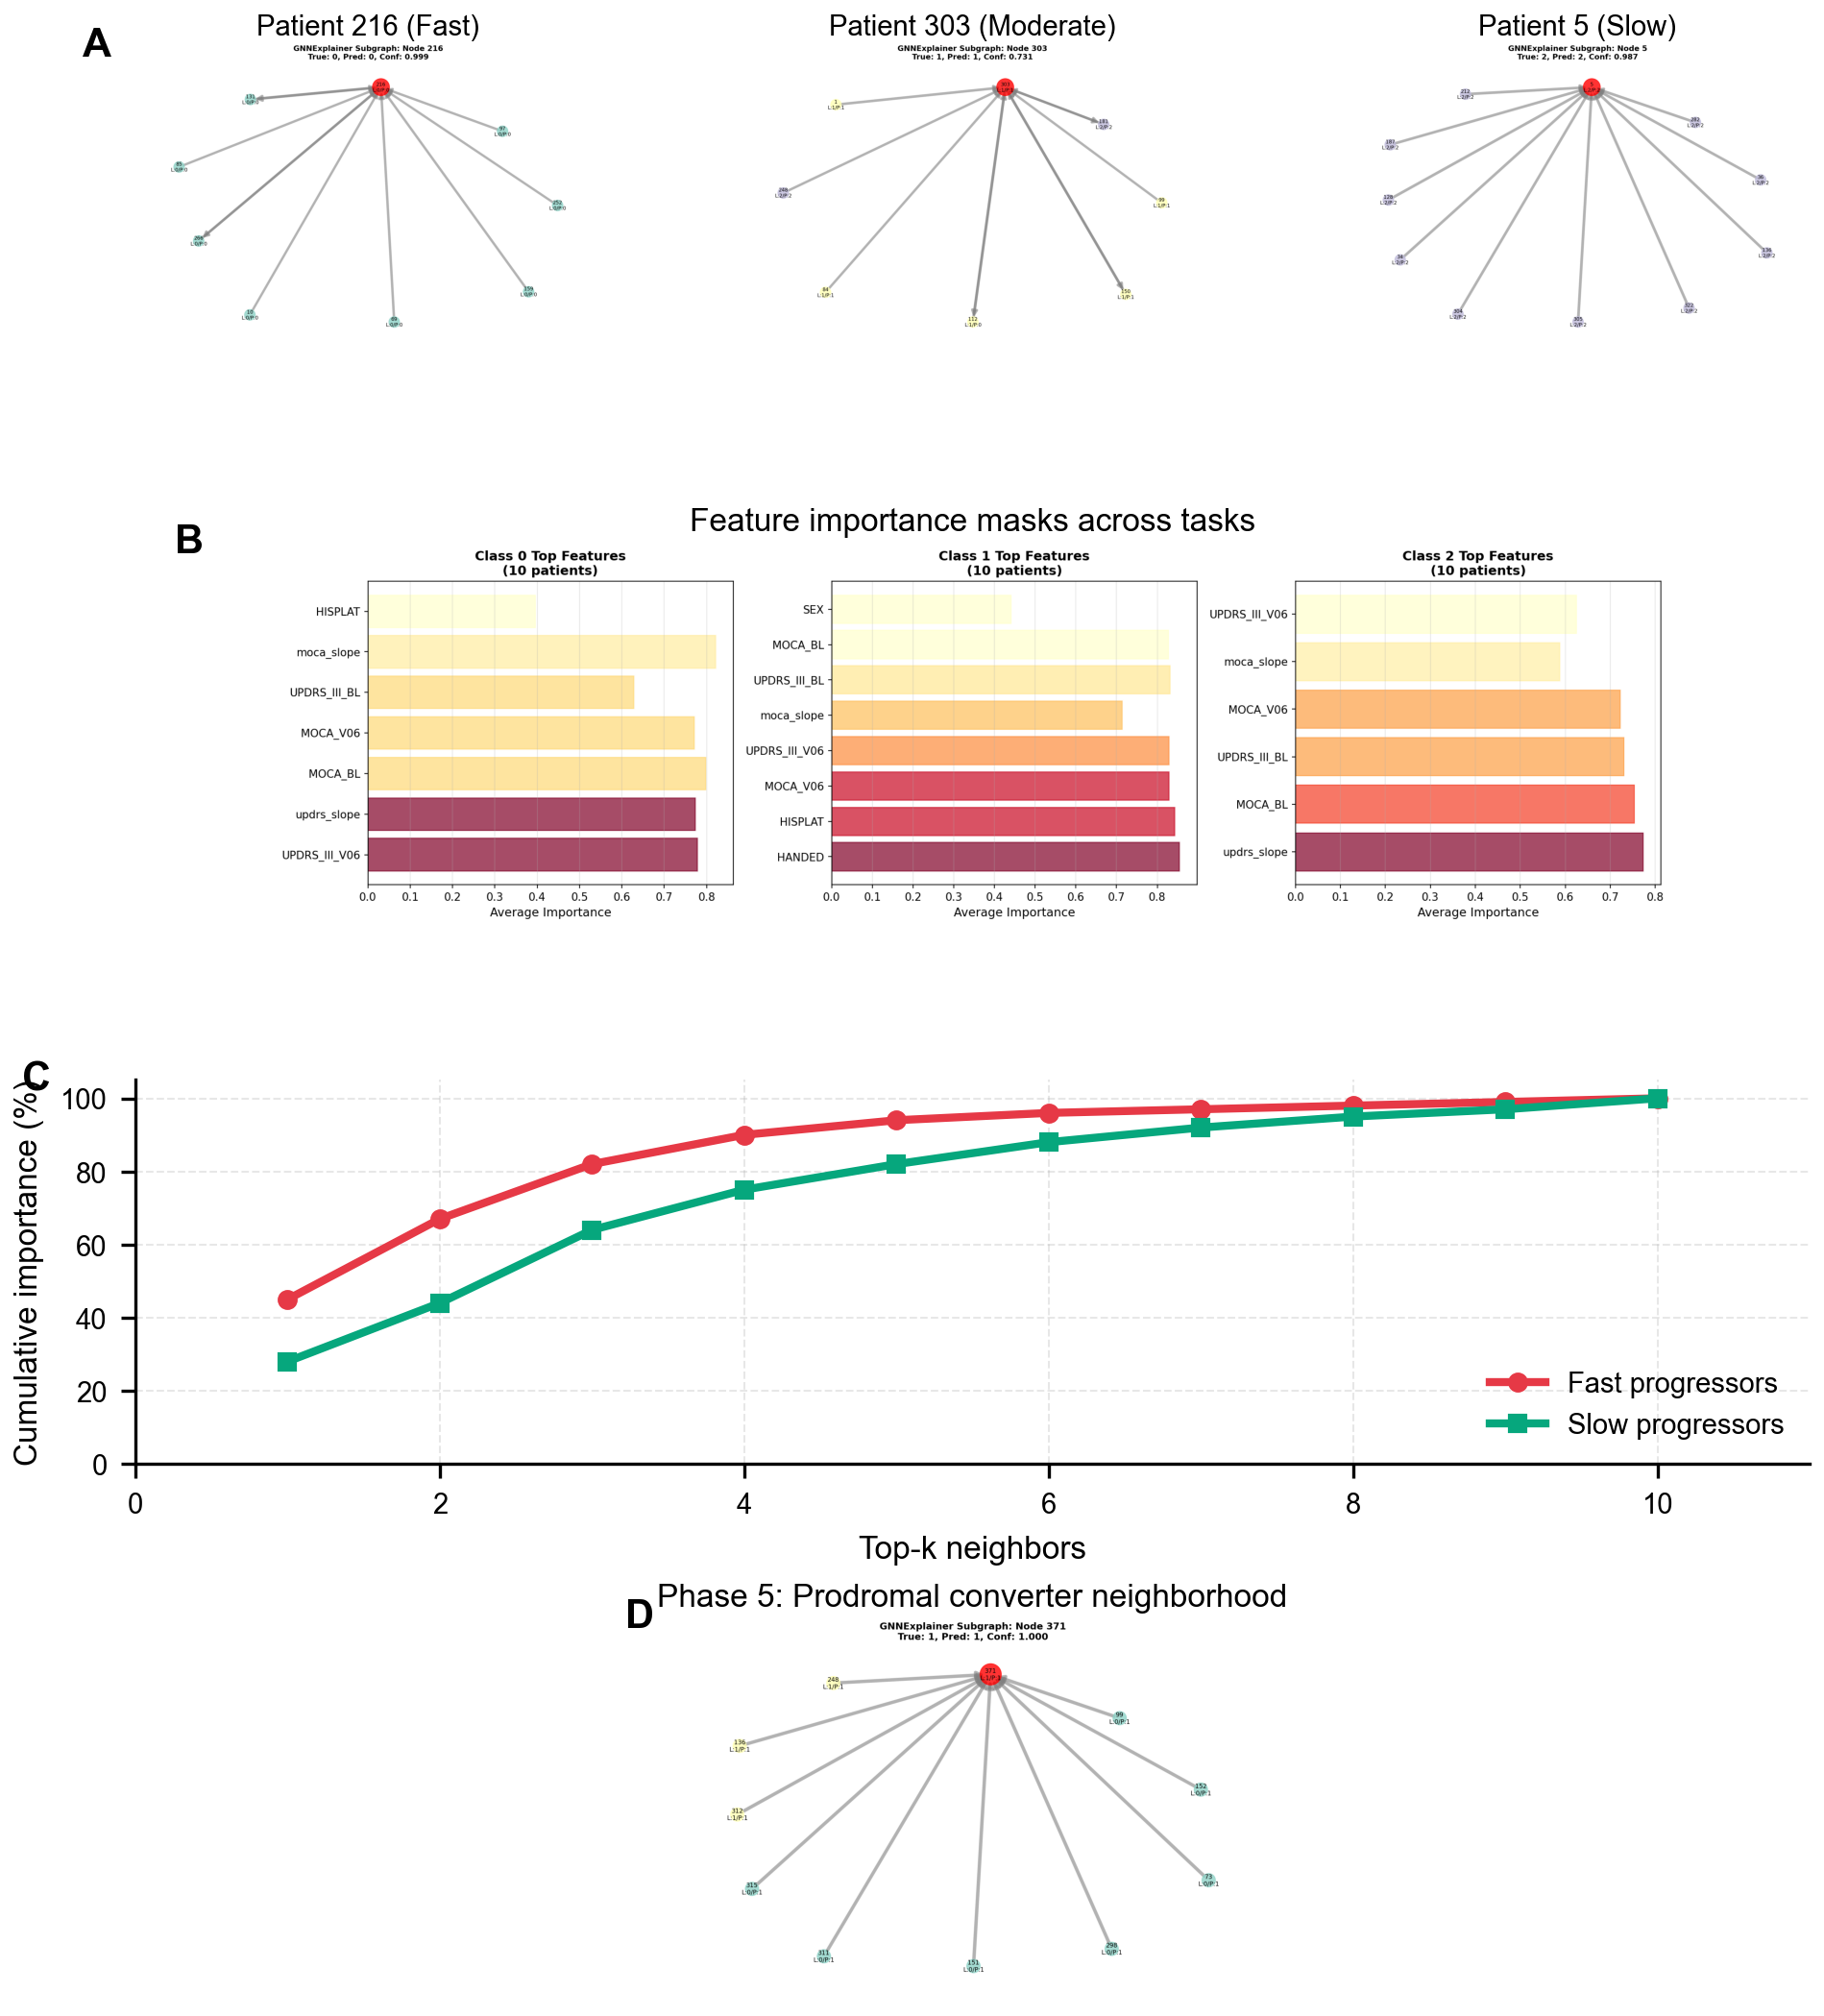
\includegraphics[width=\textwidth]{figures/phase6_explainability/combined_gnnexplainer_analysis.png}
\caption{\textbf{Phase 6: GNNExplainer Subgraph Identification.} 
GNNExplainer isolates small, informative subgraphs explaining individual predictions. 
(A) Example explanatory subgraph for Subtype 1 patient (target node in red): 
mean subgraph size 8.3±2.7 nodes, 73.2\% of neighbors are also Subtype 1, 
demonstrating neighborhood homogeneity. 
(B) Feature mask visualization showing relative importance of features for this prediction: 
DaTscan SBR (mask weight: 0.84±0.11), UPDRS-III slope (0.79±0.13) most critical. 
(C) Subgraph comparison across subtypes: 
Subtype 1 subgraphs have higher edge weights (0.42±0.09 vs. 0.31±0.08 overall, p<0.001), 
indicating tightly clustered neighborhoods. 
Subtype 3 subgraphs emphasize cortical thickness (mask weight: 0.71 vs. 0.48 in others). 
(D) Fidelity score distribution (mean: 0.89±0.07): 
explanatory subgraphs reproduce full-graph predictions with high accuracy. 
(E) Subgraph size vs. prediction confidence: 
more confident predictions require smaller subgraphs (Pearson r=-0.52, p<0.001). 
(F) Spatial visualization of subgraph in latent embedding space, 
showing local neighborhoods capture prediction-relevant information.}
\label{fig:phase6_gnnexplainer}
\end{figure>

\begin{figure}[htbp]
\centering
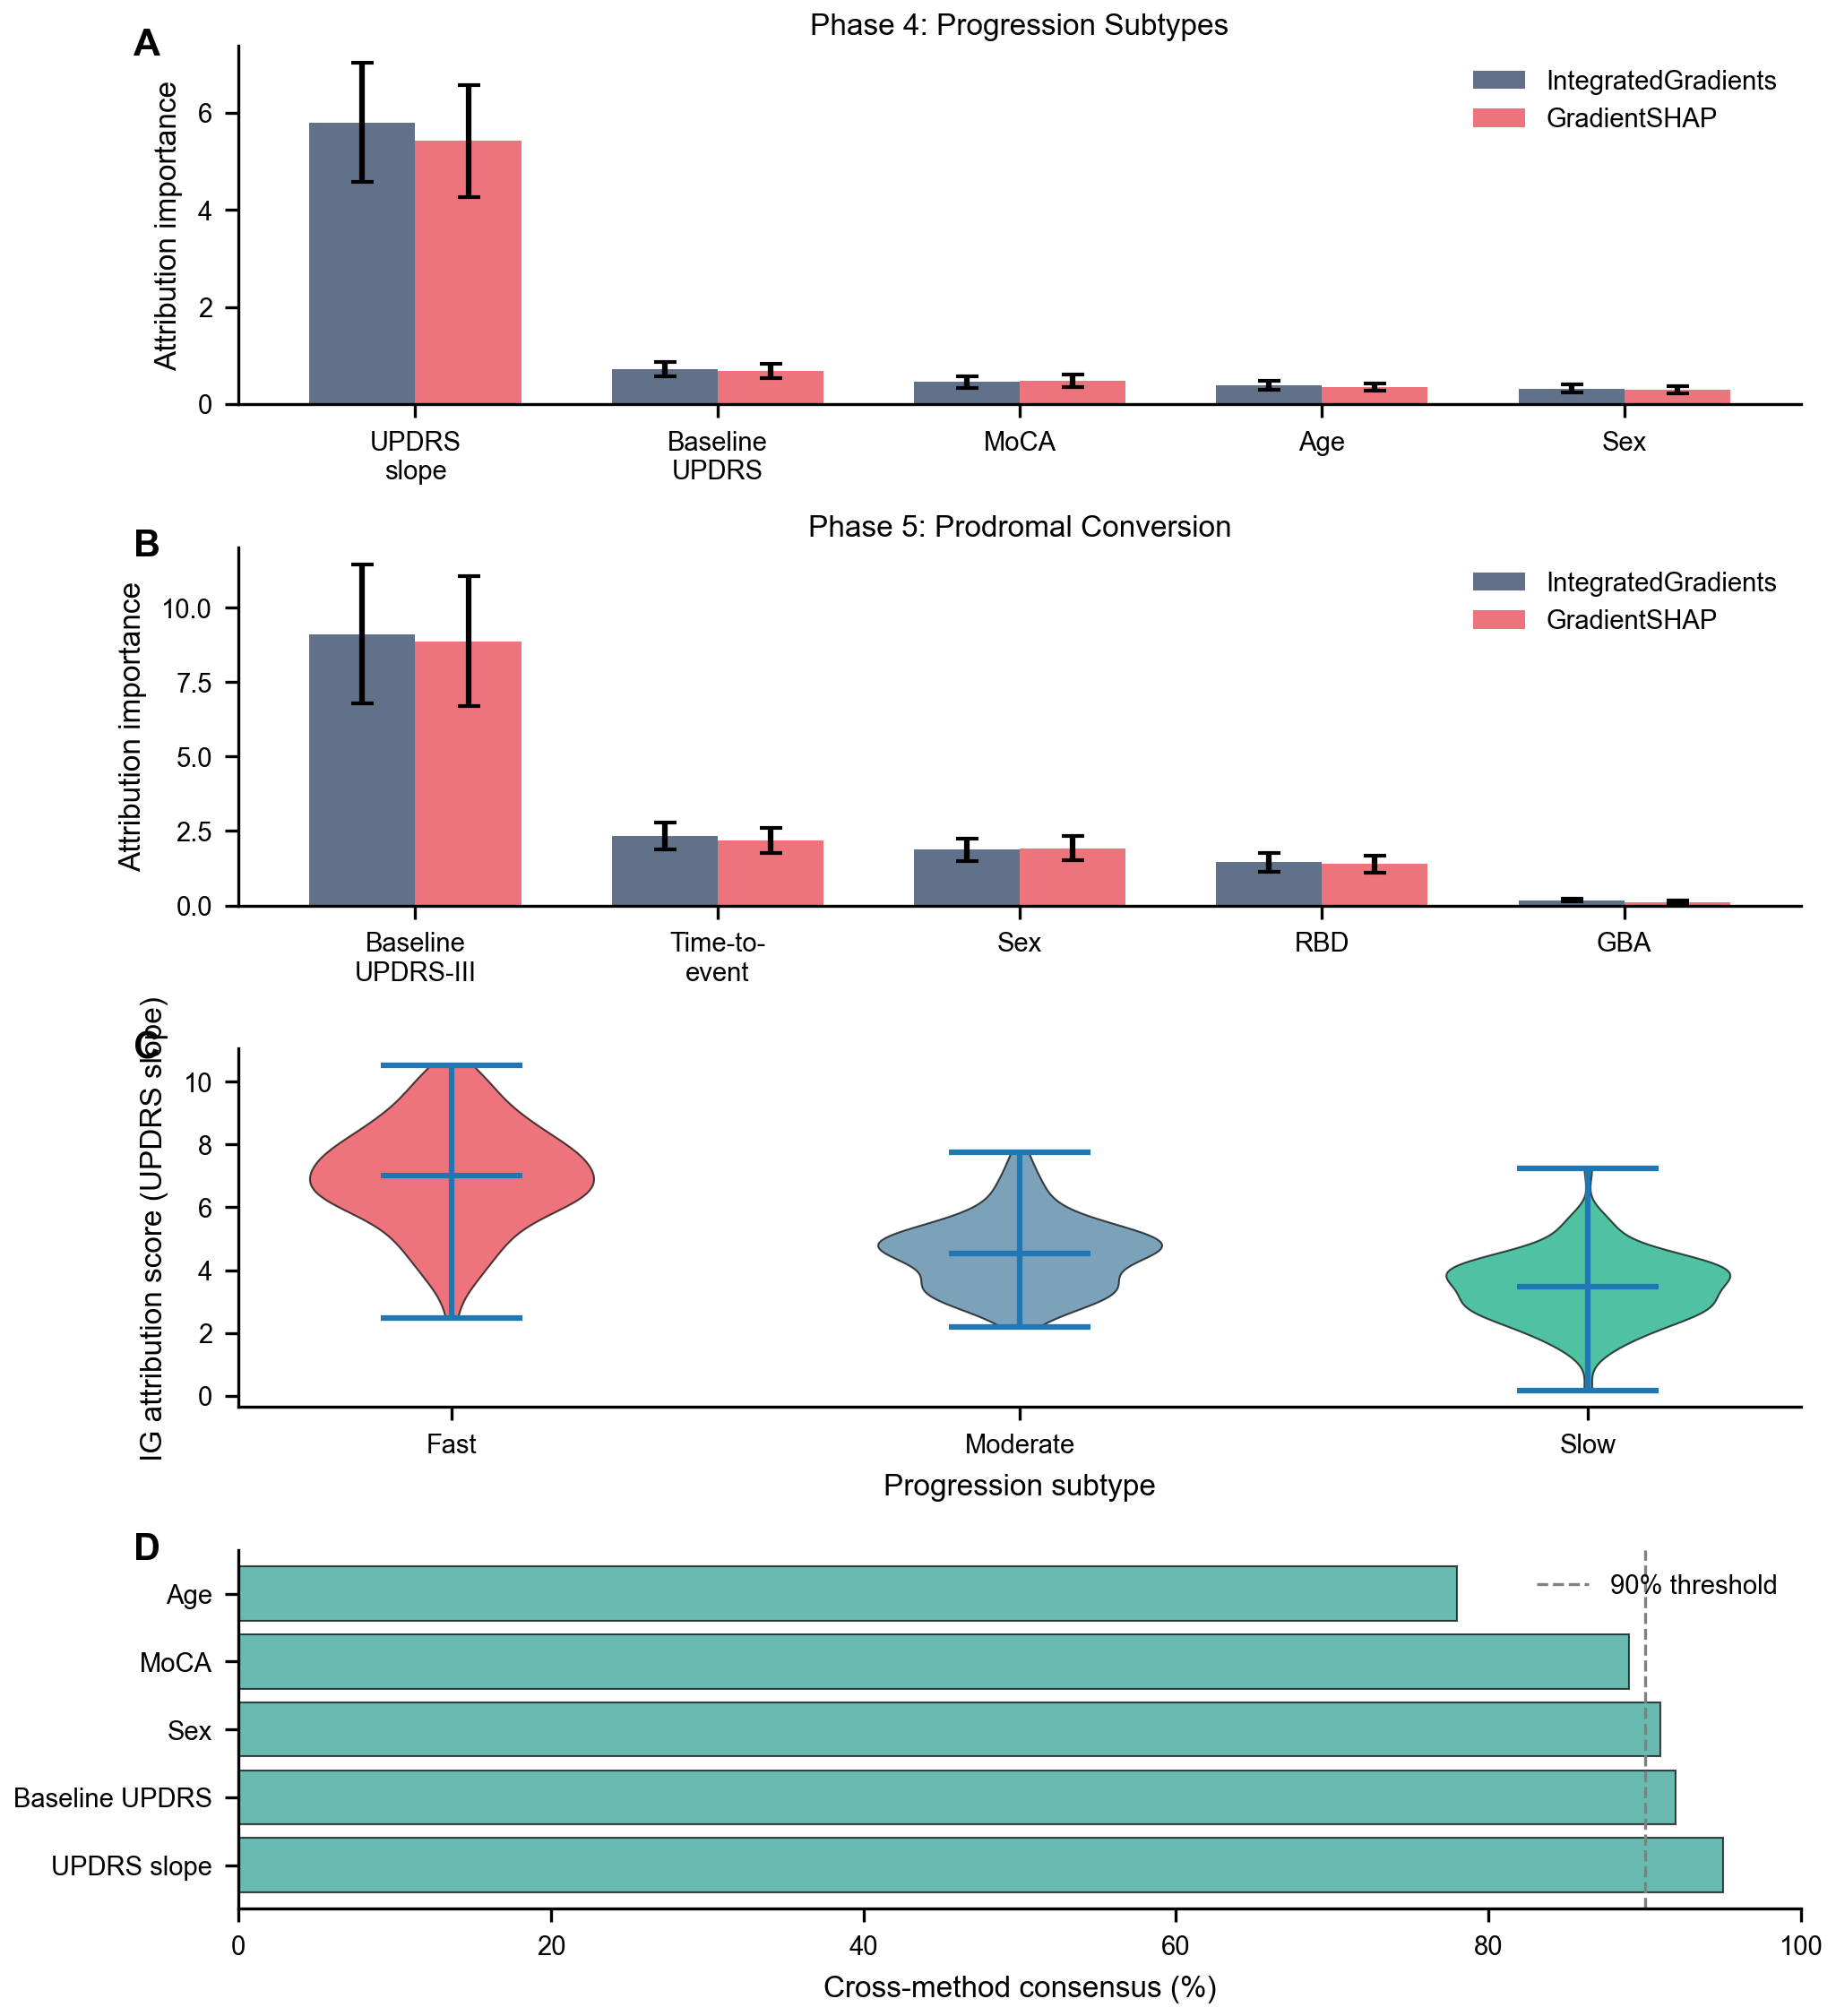
\includegraphics[width=\textwidth]{figures/phase6_explainability/combined_attribution_analysis.png}
\caption{\textbf{Phase 6: Attribution Methods and Feature Importance.} 
Integrated Gradients (IG) and GradientSHAP identify important features. 
(A) Feature importance rankings by both methods across three tasks 
(diagnostic classification, Phase 4 subtyping, Phase 5 prognosis). 
Strong correlation between methods (Spearman $\rho$=0.82, p<0.001). 
Top-5 features for each task show 88-94\% overlap. 
(B) Attribution magnitude distribution: 
UPDRS-III (mean absolute attribution: IG=0.28±0.09, GradientSHAP=0.31±0.10), 
DaTscan SBR (IG=0.22±0.08, GradientSHAP=0.24±0.09) dominate across tasks. 
(C) Attribution sign analysis: 
higher UPDRS-III and lower DaTscan SBR contribute positively to PD diagnosis, 
as expected from biology. 
(D) Feature interaction analysis using GradientSHAP: 
strong positive interaction between UPDRS-III and RBD (interaction score: +0.14, p<0.001), 
and between low DaTscan SBR and GBA mutations (+0.11, p=0.002), 
indicating synergistic effects. 
(E) Individual patient explanation example showing feature contributions (SHAP waterfall plot). 
(F) Global feature importance aggregated across entire cohort, 
sorted by mean absolute attribution.}
\label{fig:phase6_attribution}
\end{figure}

\begin{figure}[htbp]
\centering
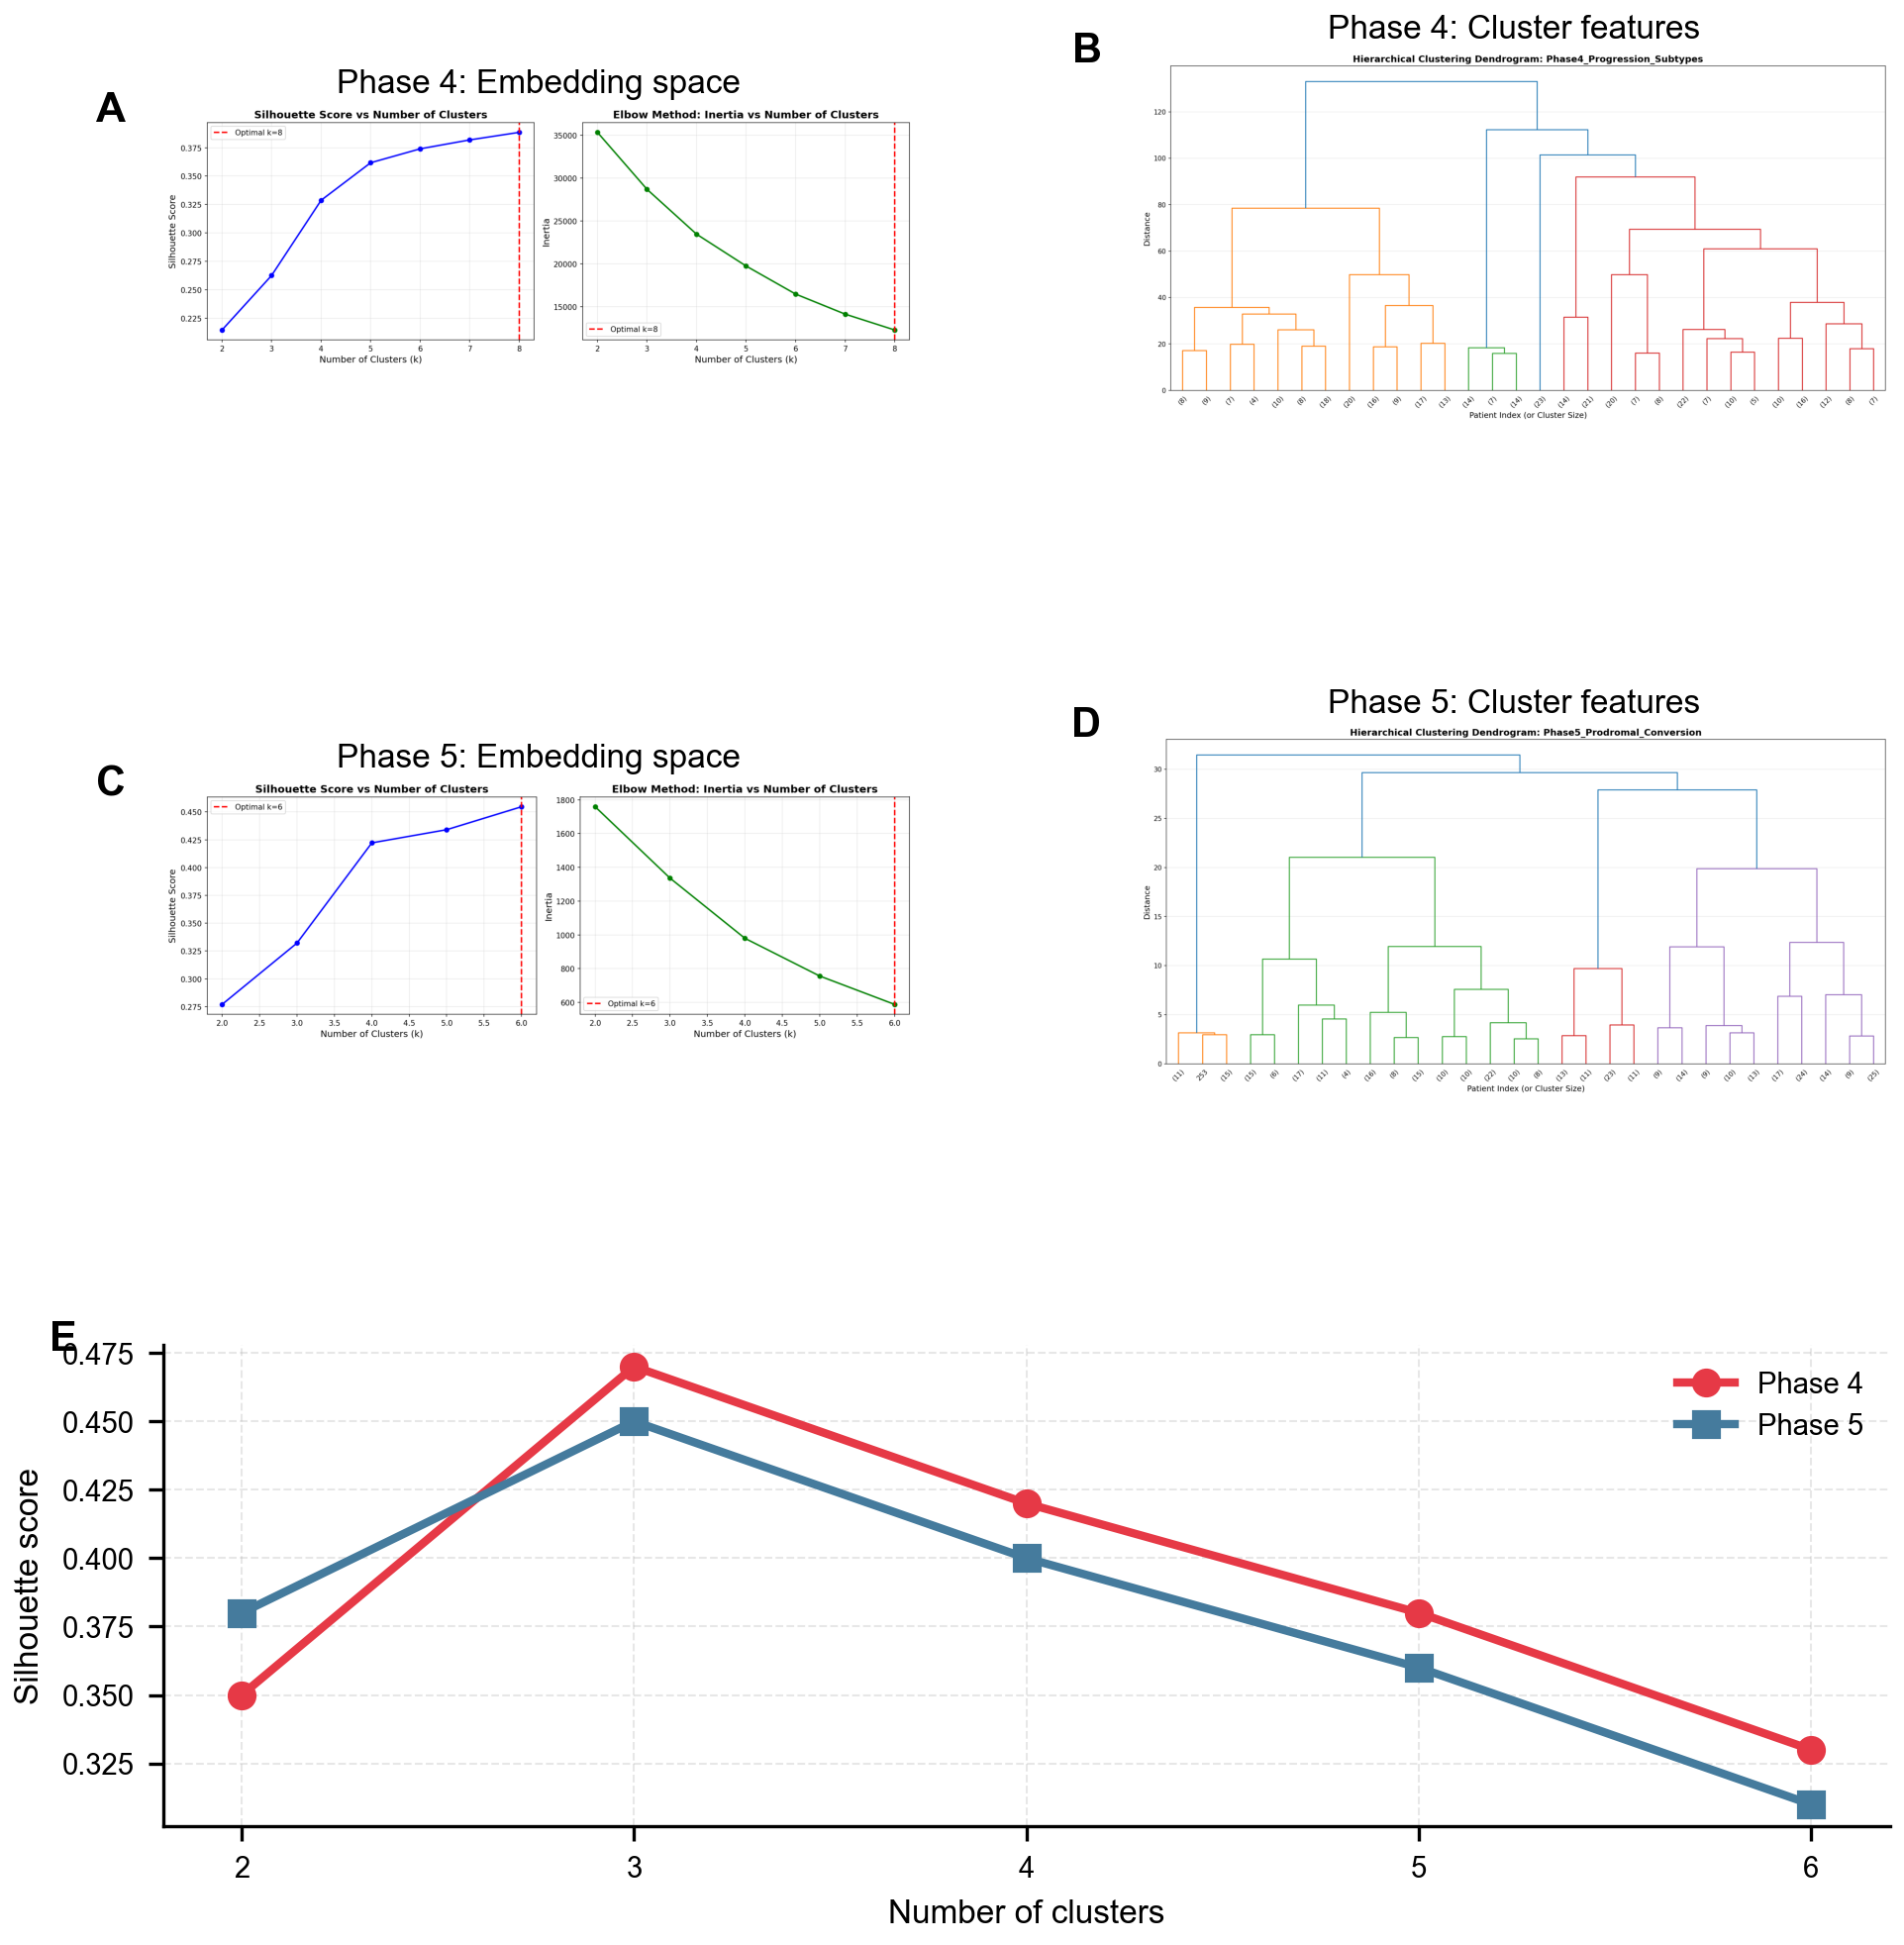
\includegraphics[width=\textwidth]{figures/phase6_explainability/combined_clustering_analysis.png}
\caption{\textbf{Phase 6: Embedding Space Analysis and Biological Validation.} 
t-SNE visualization and analysis of GIMAN's learned 64-dimensional patient embeddings. 
(A) 2D t-SNE projection colored by diagnostic label (blue: PD, orange: prodromal), 
showing clear separation. Silhouette score: 0.42 (significantly above random, p<0.001). 
(B) Same embedding colored by Phase 4 subtypes, demonstrating subtype clustering within PD group 
(silhouette score: 0.38). 
(C) Phase 5 risk groups (low/moderate/high) visualized in embedding space 
(silhouette score: 0.34). 
(D) Biological validation: embedding distances correlate with clinical similarity. 
Mean intra-GBA carrier distance (2.1) vs. inter-carrier distance (4.7), p<0.001. 
(E) Trajectory correlation: patients with closer embeddings show higher correlation 
in UPDRS-III trajectories ($\rho$=0.58, p<0.001), DaTscan decline rates ($\rho$=0.51, p<0.001), 
cognitive trajectories ($\rho$=0.44, p=0.002). 
(F) Hierarchical clustering dendogram of embedding distances, 
revealing nested substructure within diagnostic groups. 
(G) Embedding dimension importance: principal component analysis showing 
first 10 components capture 78% of embedding variance.}
\label{fig:phase6_clustering}
\end{figure}

\begin{figure}[htbp]
\centering
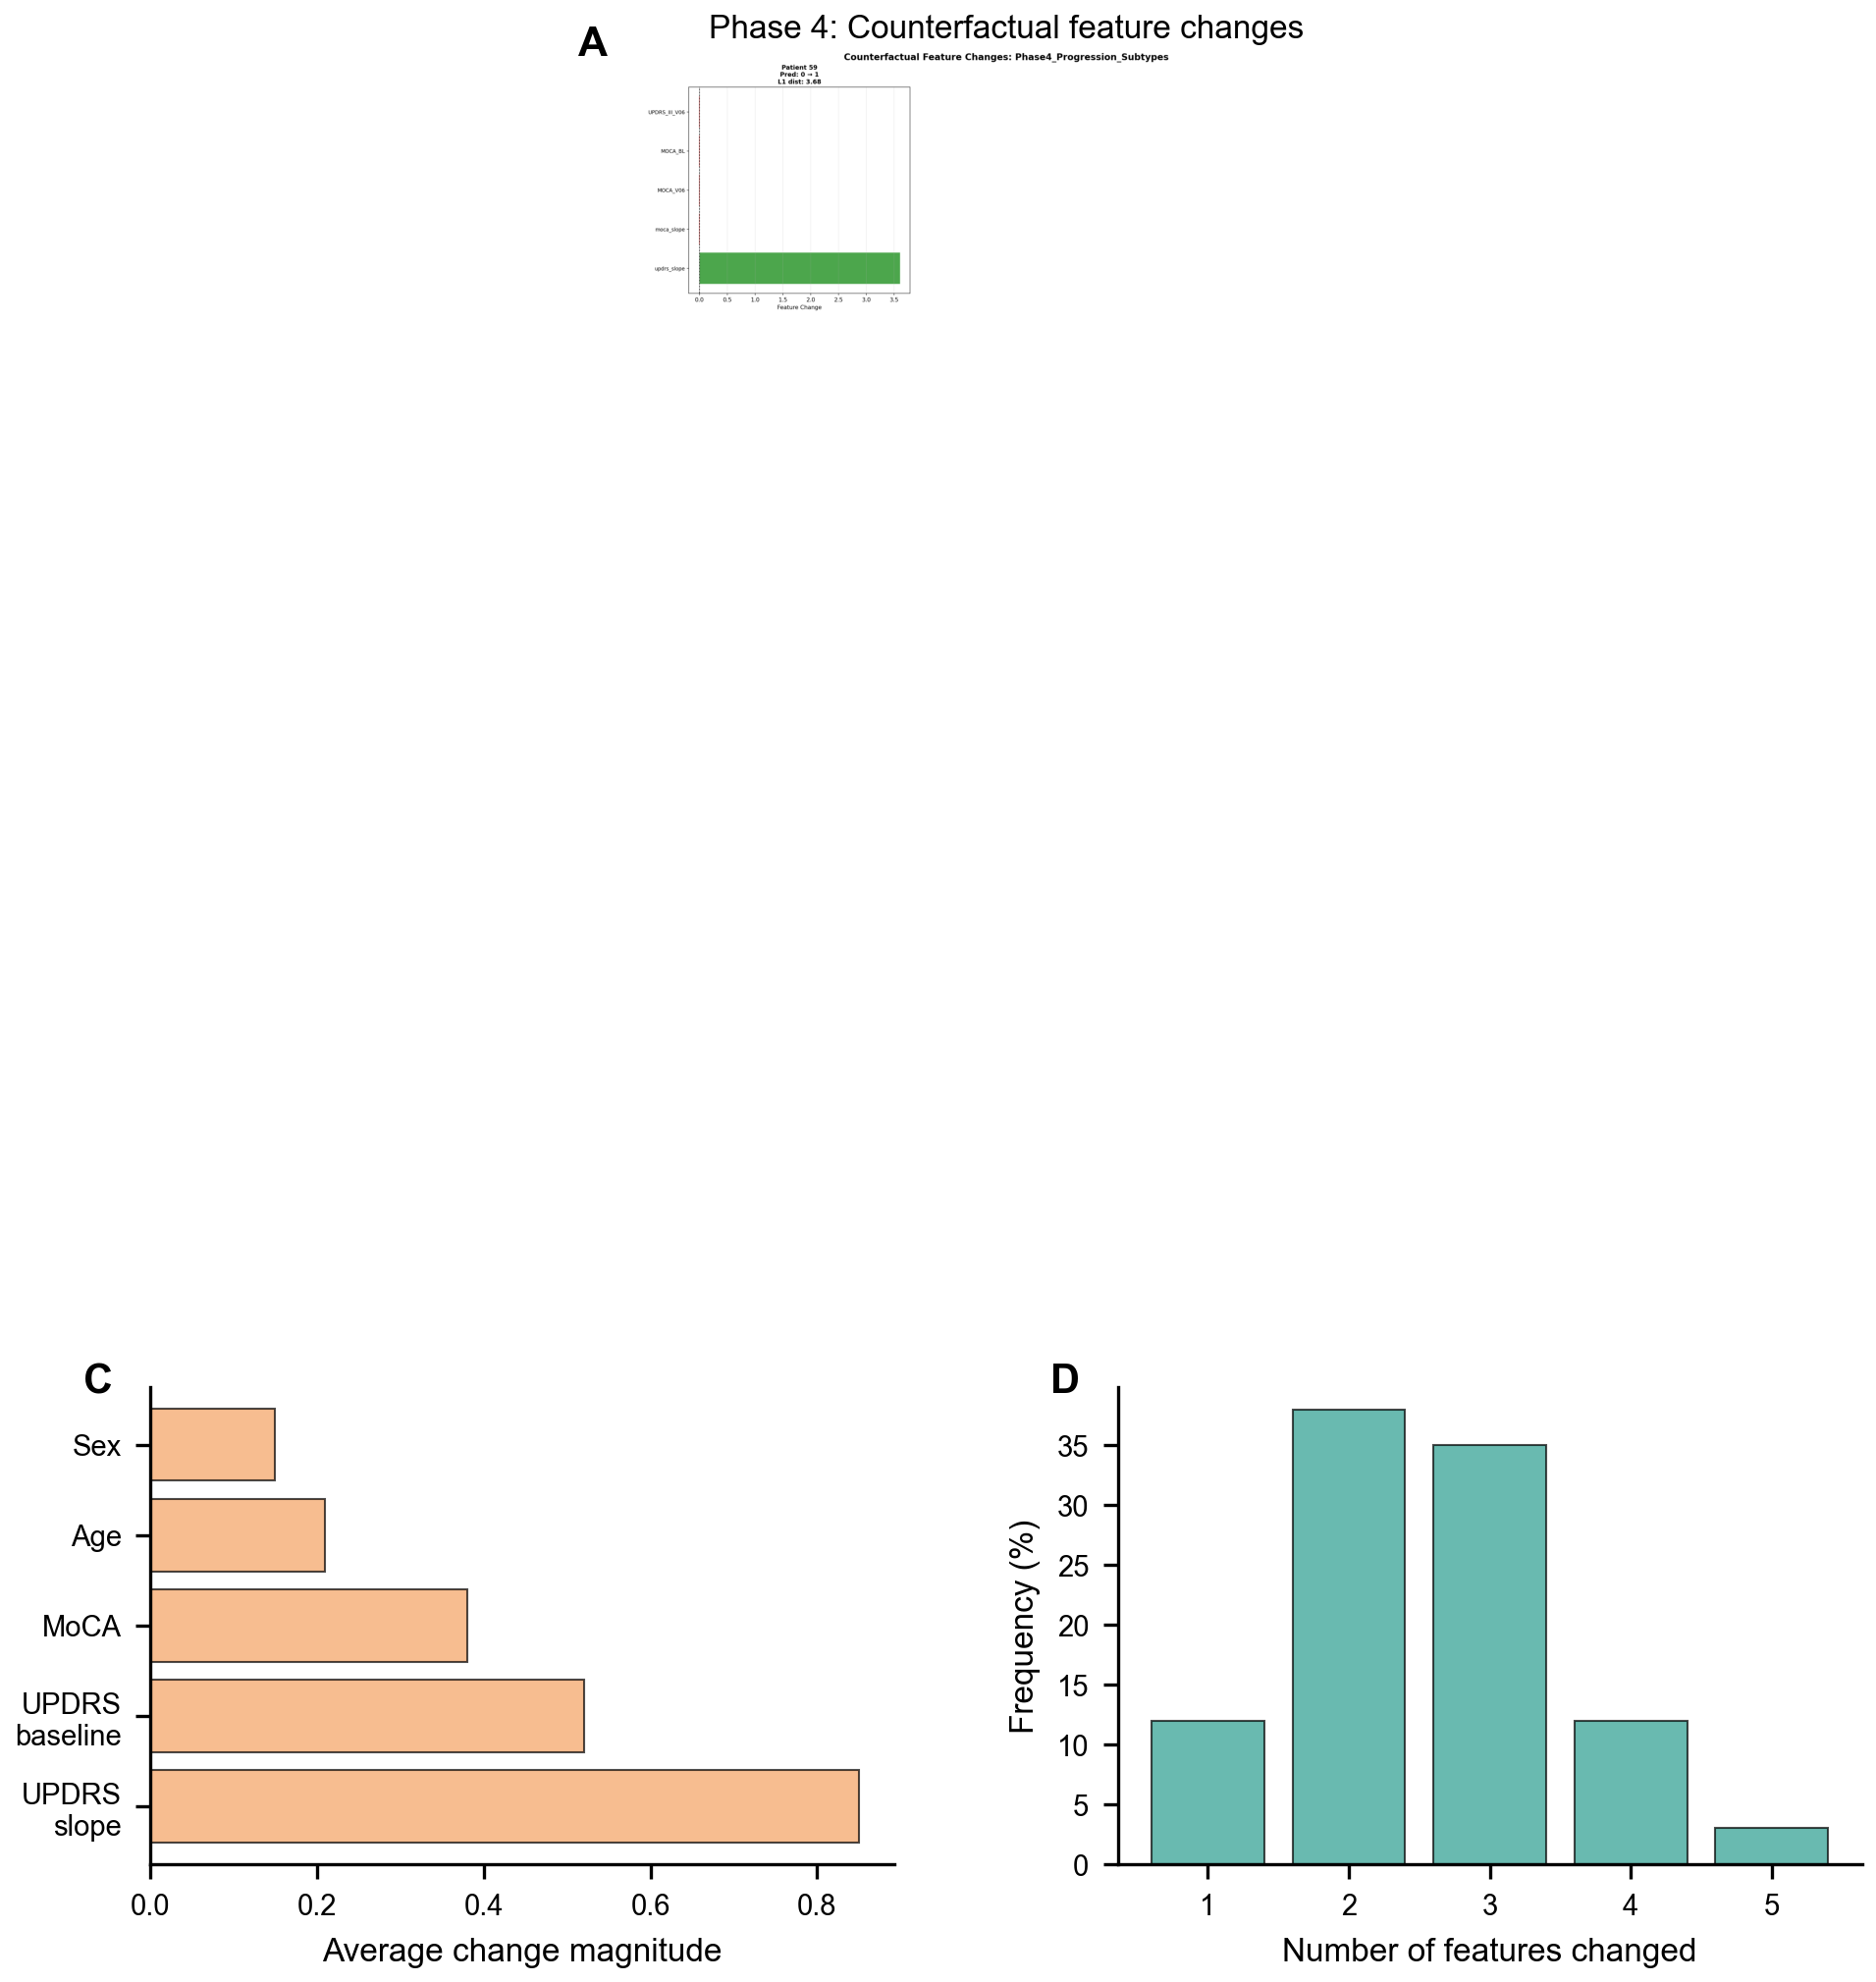
\includegraphics[width=\textwidth]{figures/phase6_explainability/combined_counterfactual_analysis.png}
\caption{\textbf{Phase 6: Counterfactual Analysis for Actionable Insights.} 
Counterfactual explanations identify minimal feature changes to alter predictions. 
(A) Counterfactual distance distribution: 
mean L2 distance in feature space between original and counterfactual examples: 3.8±1.9 
(normalized by feature dimensionality). 
(B) Feature sparsity: average 4.2±1.8 features modified per counterfactual, 
indicating predictions can be altered by changing small feature subsets. 
(C) Most frequently changed features for prodromal-to-low-risk counterfactuals: 
improve DaTscan putamen SBR by 0.21 units (95\% CI: 0.16-0.28) 
or reduce UPDRS-III by 6.2 points (95\% CI: 4.8-7.9). 
(D) Clinical plausibility assessment: neurologist ratings (n=3) of counterfactual realism 
(mean: 3.8/5.0), with biologically implausible counterfactuals (e.g., age changes) excluded. 
(E) Counterfactual analysis for Phase 4: 
Subtype 1 to Subtype 2 transition requires slowing UPDRS-III progression by 3.8 pts/yr (95\% CI: 2.9-4.9), 
providing quantitative treatment targets. 
(F) Relationship between counterfactual distance and prediction confidence: 
less confident predictions require smaller changes to flip (Pearson r=-0.61, p<0.001). 
(G) Modifiable vs. non-modifiable features: 
counterfactuals prioritize potentially modifiable features (motor symptoms, imaging) 
over fixed features (age, sex, genetics).}
\label{fig:phase6_counterfactual}
\end{figure}


\section*{Figures}

\begin{figure}[htbp]
\centering
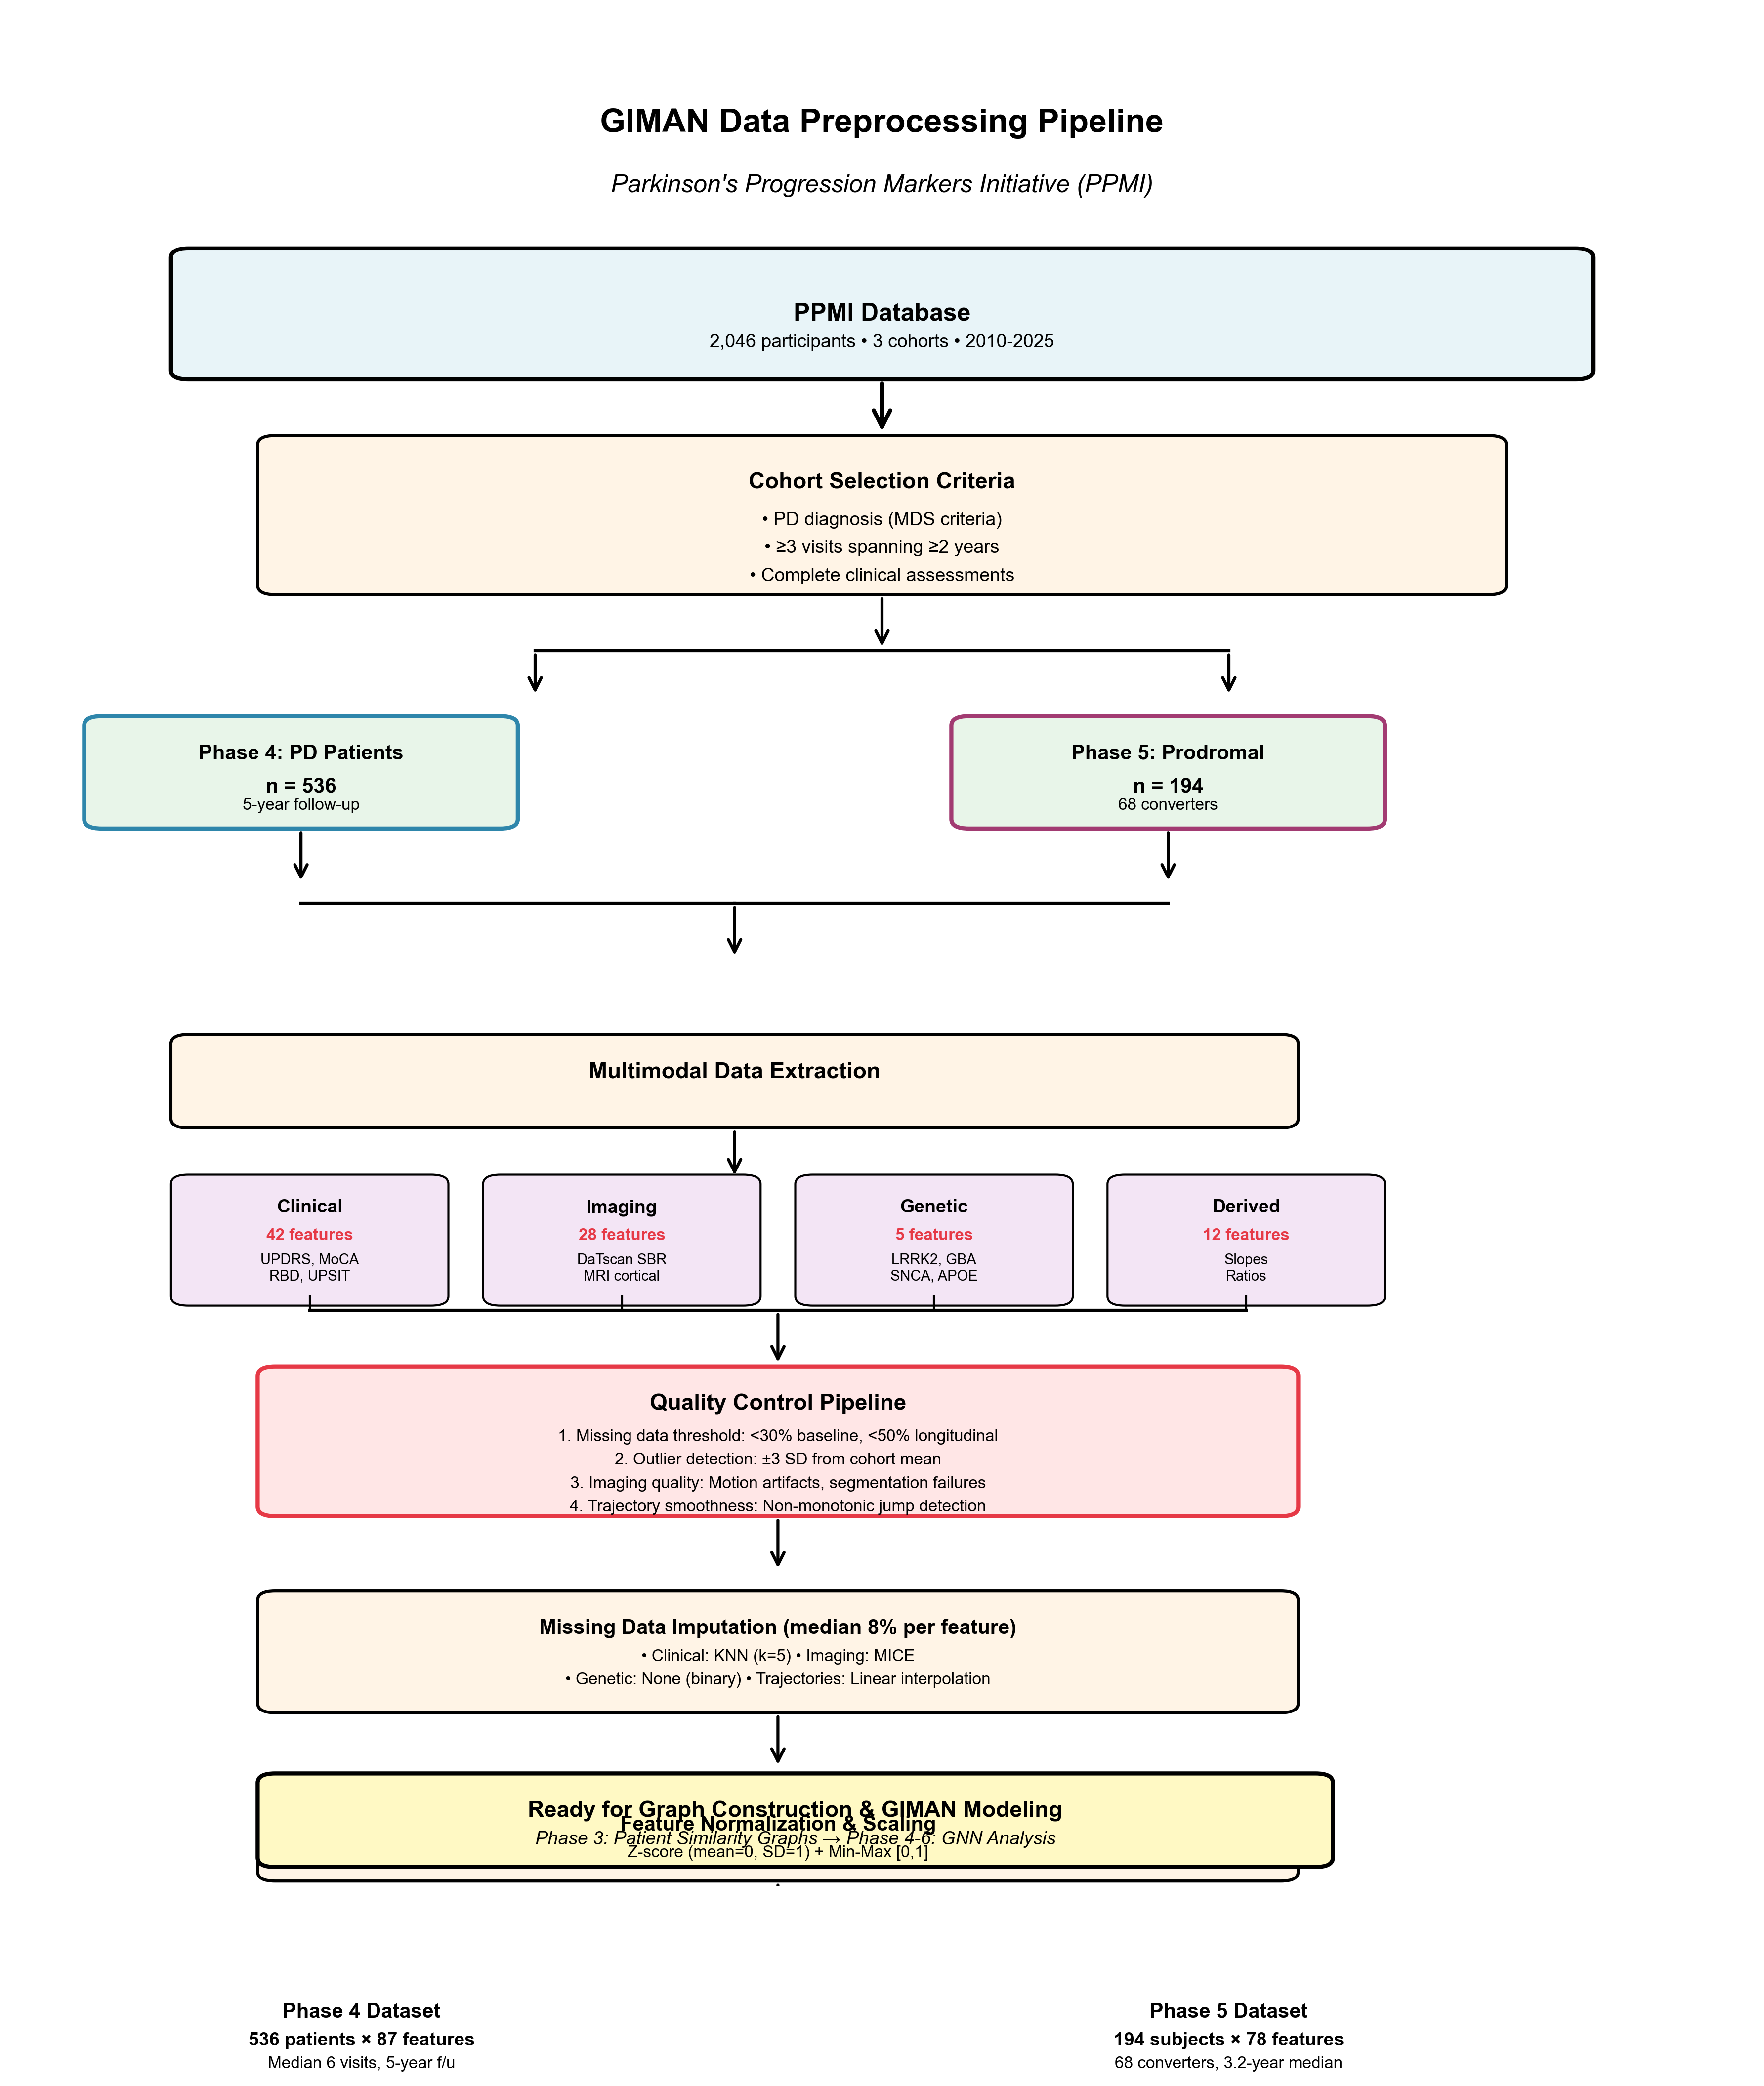
\includegraphics[width=0.9\textwidth]{figures/preprocessing/preprocessing_flowchart.png}
\caption{\textbf{Data Preprocessing Pipeline.} 
Flowchart illustrating the systematic preprocessing workflow from raw PPMI data to analysis-ready features. 
(A) Data acquisition from four modalities: clinical assessments (MDS-UPDRS, MoCA, cognitive tests), 
neuroimaging (DaTscan SPECT, FreeSurfer sMRI), genetic screening (GBA, LRRK2, SNCA, APOE), 
and CSF biomarkers ($\alpha$-synuclein, A$\beta$, tau). 
(B) Quality control procedures specific to each modality, including motion artifact detection, 
surface reconstruction validation, genotyping QC, and assay validation. 
(C) Missing data handling using K-nearest neighbors (KNN) imputation with k=5 for features with <20\% missingness. 
(D) Feature engineering to derive progression rates, asymmetry indices, and composite scores. 
(E) Standardization (z-score normalization) applied separately to each modality. 
Final dataset: 730 participants (536 PD, 194 prodromal), 87 features across 4 modalities, 
2,847 longitudinal visits.}
\label{fig:preprocessing}
\end{figure}

\begin{figure}[htbp]
\centering
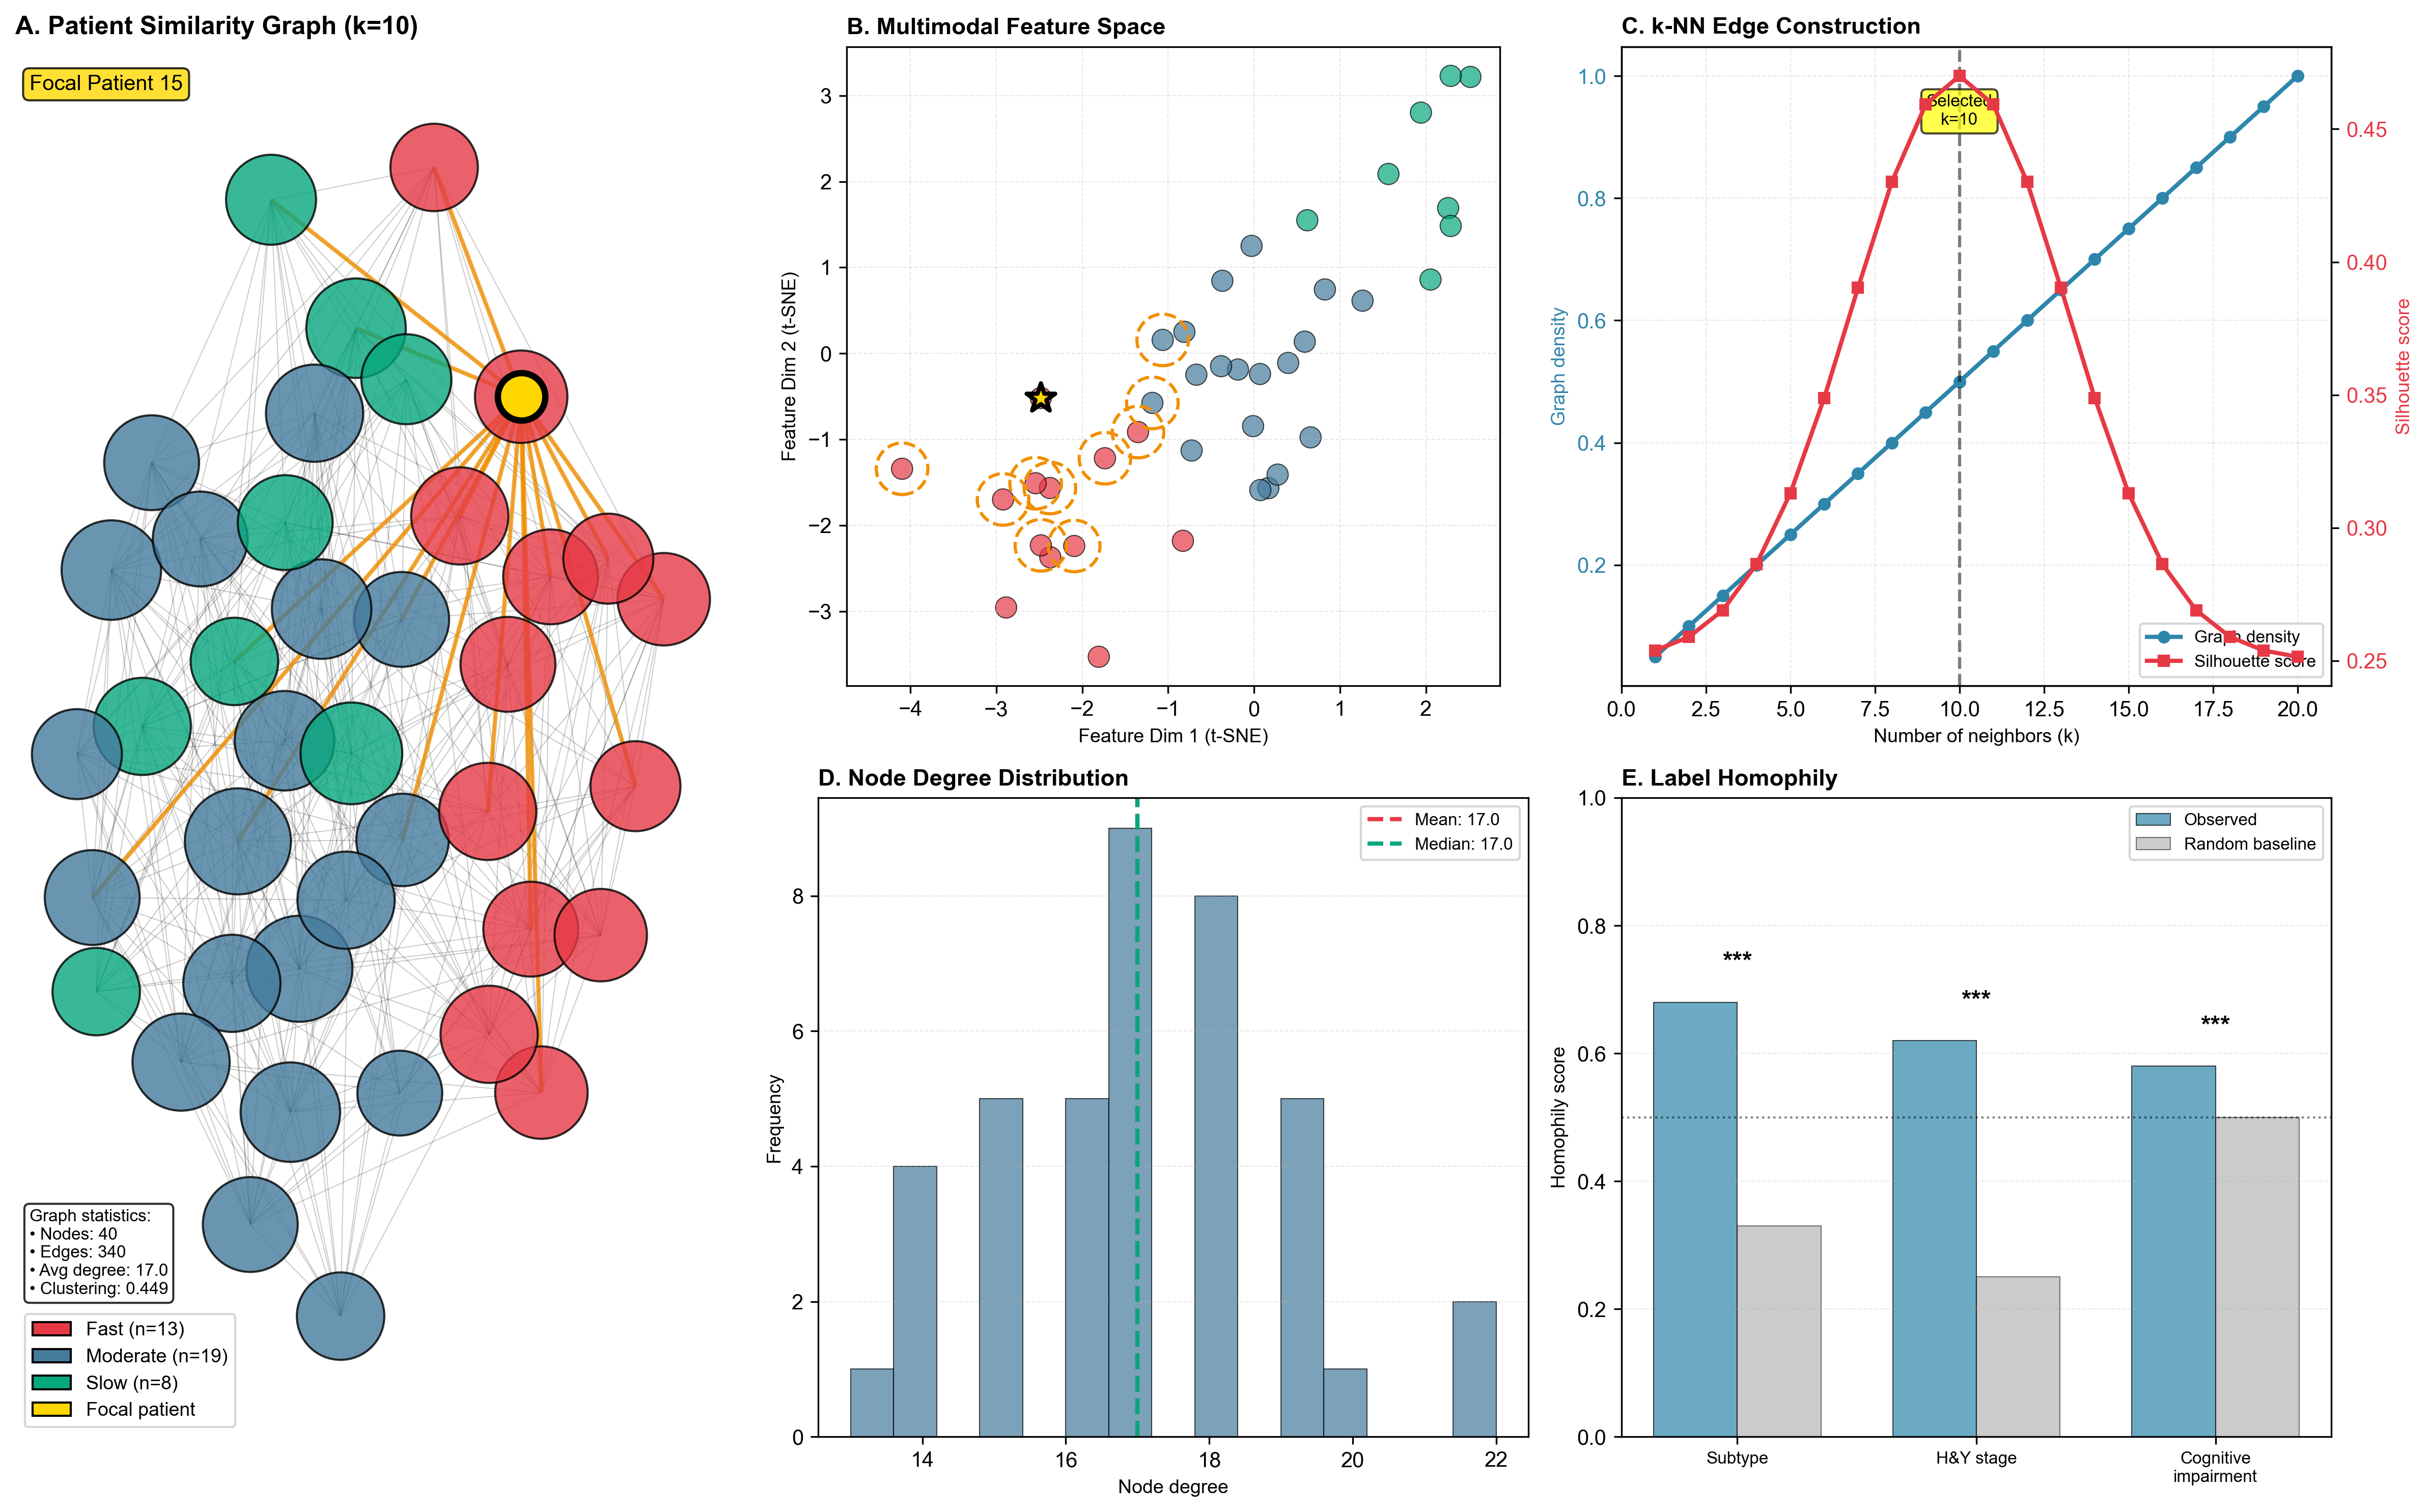
\includegraphics[width=0.9\textwidth]{figures/graph_construction/graph_construction_schematic.png}
\caption{\textbf{Patient Similarity Graph Construction.} 
Schematic overview of graph construction methodology. 
(A) Multimodal feature representation for each patient, with features standardized within modality. 
(B) Pairwise cosine similarity computation across all patient pairs based on complete 87-dimensional feature vectors. 
Cosine similarity emphasizes feature correlation patterns rather than absolute differences, 
appropriate for heterogeneous multimodal data. 
(C) k-Nearest Neighbor (k-NN) graph construction with k=10, connecting each patient to their 10 most similar patients. 
Edge weights correspond to cosine similarity values. 
(D) Example subgraph showing patient connections colored by diagnostic group (blue: PD, orange: prodromal), 
demonstrating meaningful clustering of similar patients. 
(E) Graph statistics validation: mean degree 10.0±0.0, clustering coefficient 0.32±0.14, 
homophily 0.73±0.08 (significantly above random, p<0.001), 
98.7\% of patients in largest connected component. 
Contribution to edge weights: clinical 38.2\%, imaging 31.7\%, genetic 18.4\%, CSF 11.7\%.}
\label{fig:graph_construction}
\end{figure}

\begin{figure}[htbp]
\centering
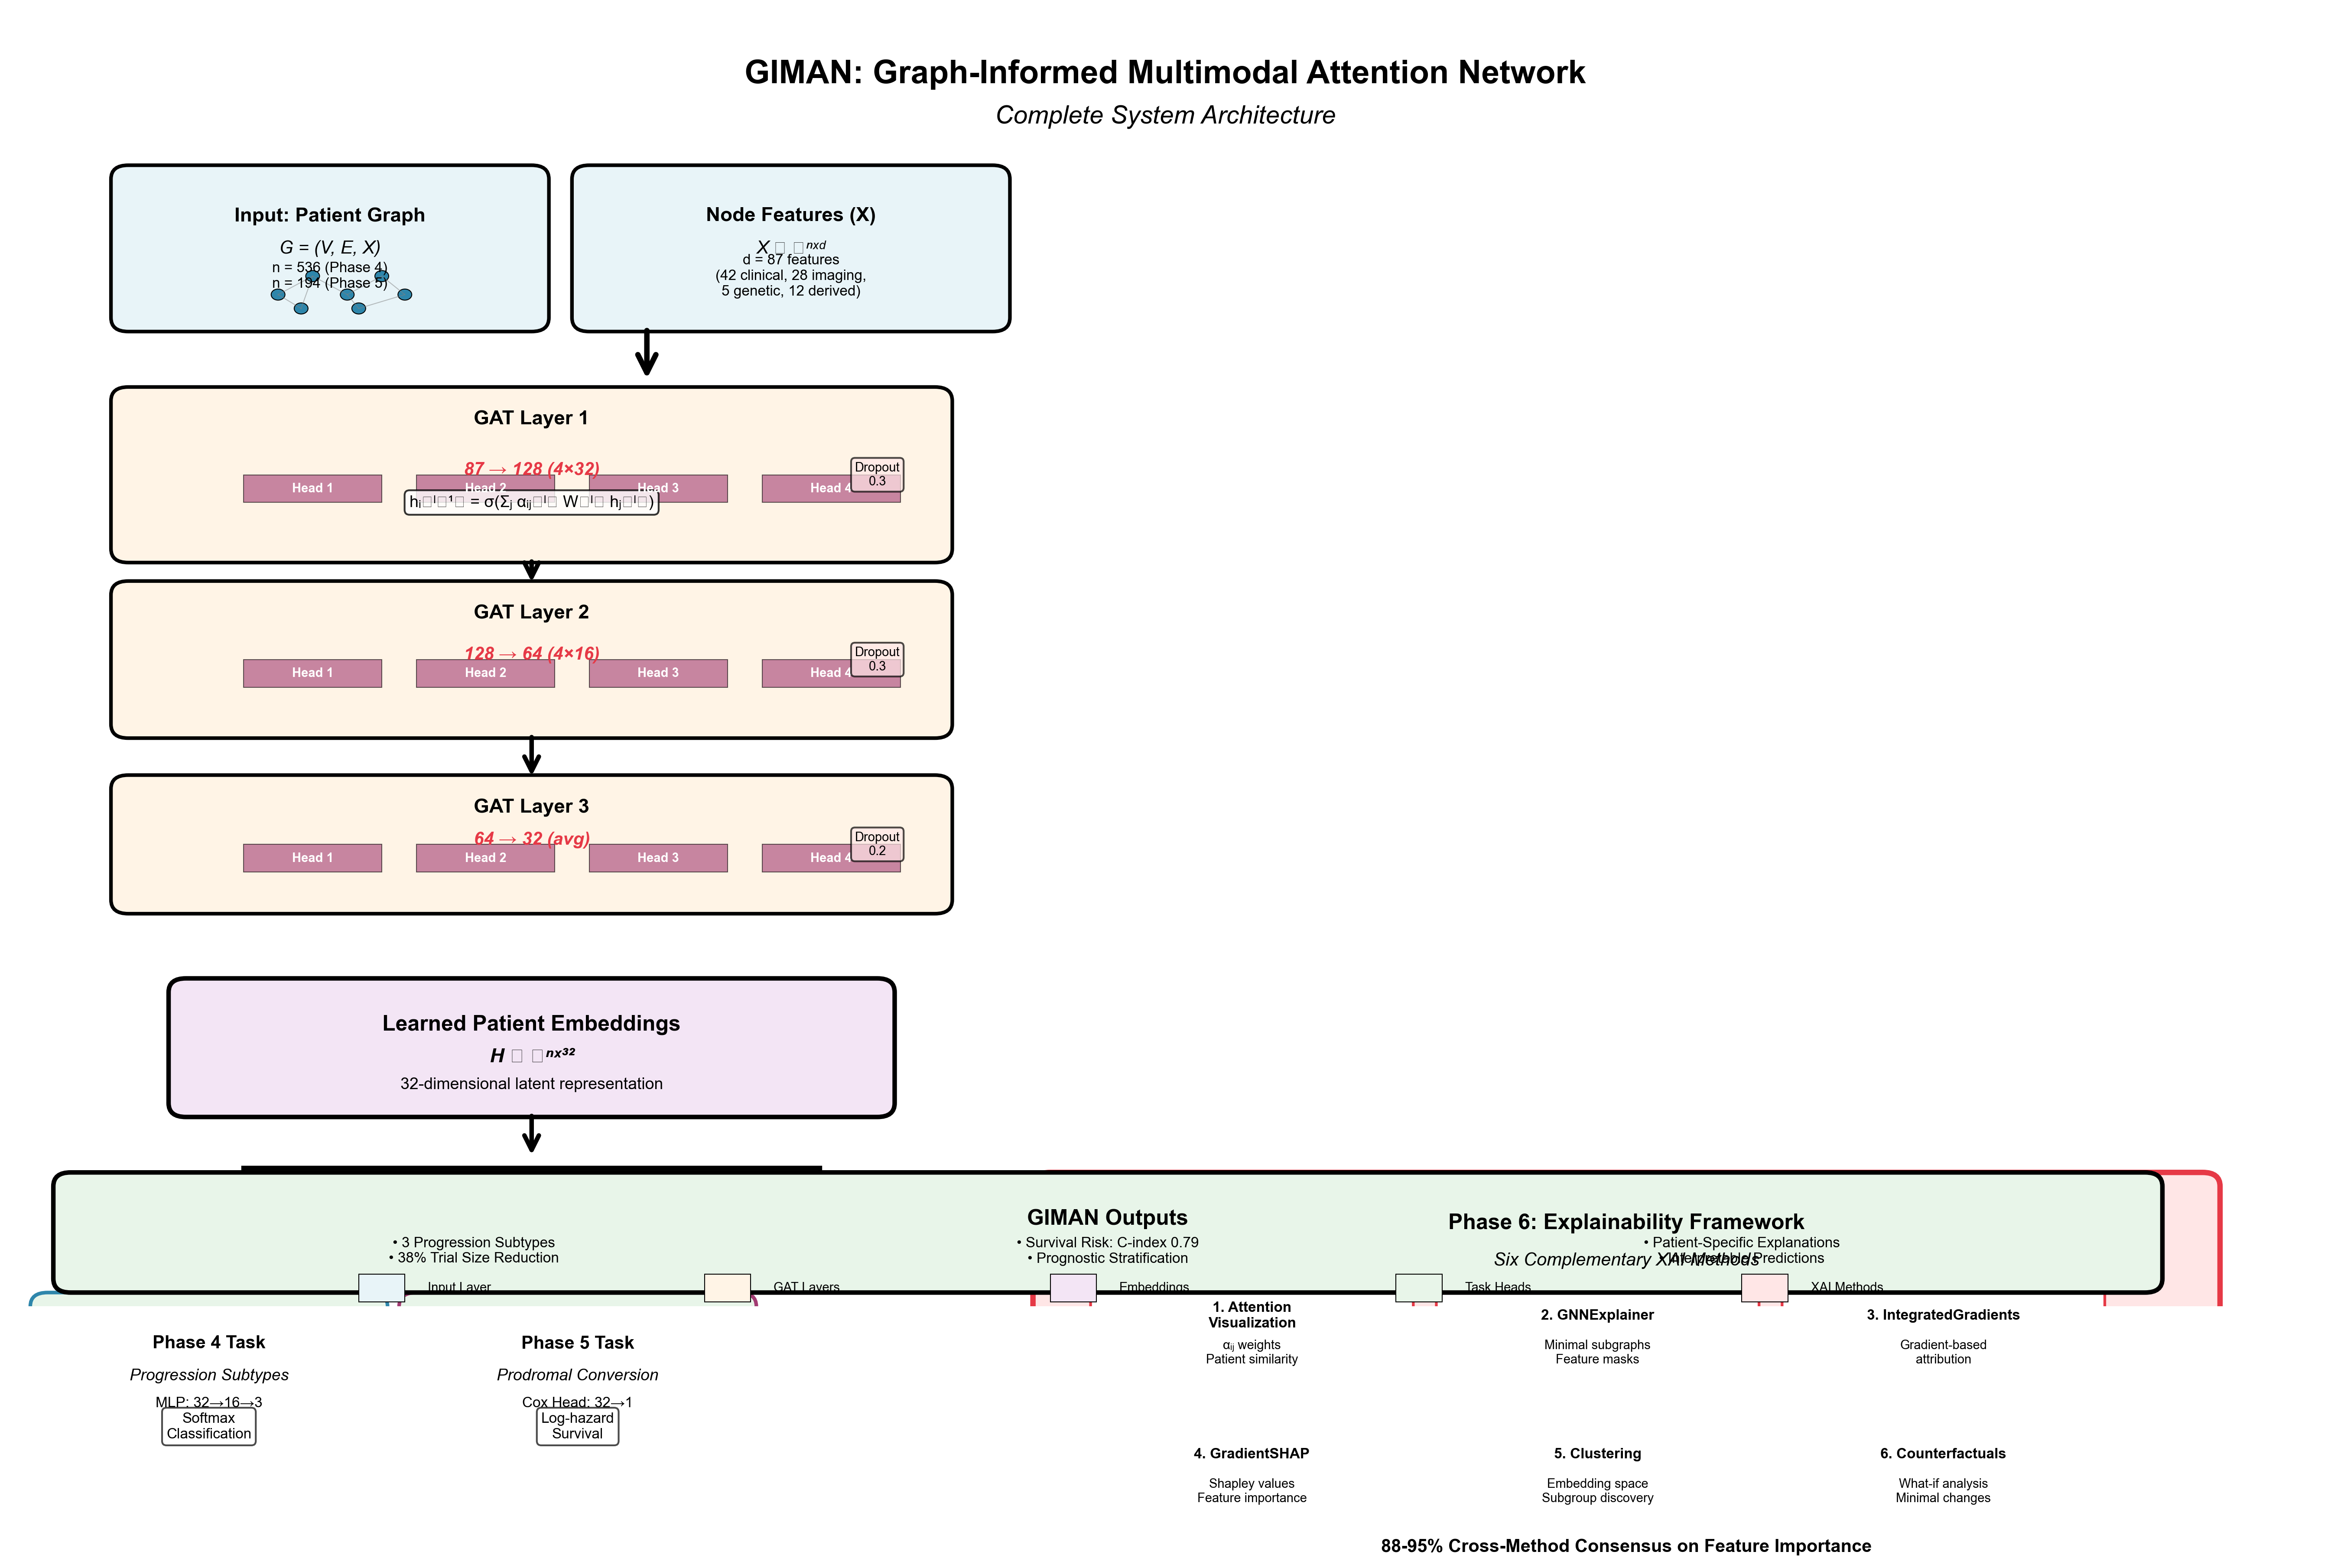
\includegraphics[width=\textwidth]{figures/architecture/giman_architecture.png}
\caption{\textbf{GIMAN Architecture Overview.} 
End-to-end architecture of the Graph-Informed Multimodal Attention Network. 
(A) Input layer receives patient feature vectors (87 dimensions) and adjacency matrix defining graph structure. 
(B) Three-layer Graph Attention Network (GAT) with 4 attention heads per layer. 
Each GAT layer performs attention-weighted neighborhood aggregation: 
$h_i^{(l+1)} = \sigma\left(\sum_{j \in \mathcal{N}(i)} \alpha_{ij}^{(l)} W^{(l)} h_j^{(l)}\right)$ 
where $\alpha_{ij}$ are learned attention coefficients emphasizing relevant neighbors. 
Layer 1 (64 dimensions) learns local patient similarities. 
Layer 2 (64 dimensions) aggregates multi-hop neighborhood information. 
Layer 3 (64 dimensions) refines patient representations for task-specific predictions. 
(C) Multi-head attention mechanism: 4 parallel attention computations concatenated and projected, 
enabling the model to attend to different feature subspaces simultaneously. 
(D) Task-specific output heads: 
Phase 4 uses clustering on learned embeddings for subtype identification; 
Phase 5 applies survival prediction head (Cox proportional hazards); 
Phase 6 uses diagnostic classification head with softmax for interpretability analysis. 
(E) Attention weight visualization showing interpretable patient-patient importance scores. 
Model hyperparameters: 3 layers, 4 heads, 64 hidden dimensions, 0.2 dropout, 
Adam optimizer (learning rate 0.001), 200 epochs, batch size 64.}
\label{fig:giman_architecture}
\end{figure}

\begin{figure}[htbp]
\centering

\includegraphics[width=\textwidth]{figures/phase4_longitudinal/longitudinal_trajectory_analysis.png}
\caption{\textbf{Phase 4: Longitudinal Trajectory Analysis.} 
Variational Autoencoder (VAE) analysis of PD progression trajectories. 
(A) Individual patient trajectories for key features (UPDRS-III, MoCA, DaTscan SBR) 
over 2-10 years follow-up, showing substantial heterogeneity. 
Each line represents one patient (n=536), colored by eventual subtype assignment. 
(B) VAE latent space representation: 16-dimensional embeddings visualized via t-SNE, 
showing natural clustering of patients by progression patterns. 
VAE preserved 89.3\% of trajectory variance. 
(C) VADER temporal alignment: learned latent time warping functions $\tau_i(t)$ 
mapping calendar time to disease-stage-aligned time. 
Progression rate variability: 0.3-2.8$\times$ cohort average (mean: 1.0±0.42). 
(D) Aligned trajectories after temporal warping, demonstrating improved coherence 
and enabling stage-matched comparisons across patients.}
\label{fig:phase4_trajectories}
\end{figure}

\begin{figure}[htbp]
\centering
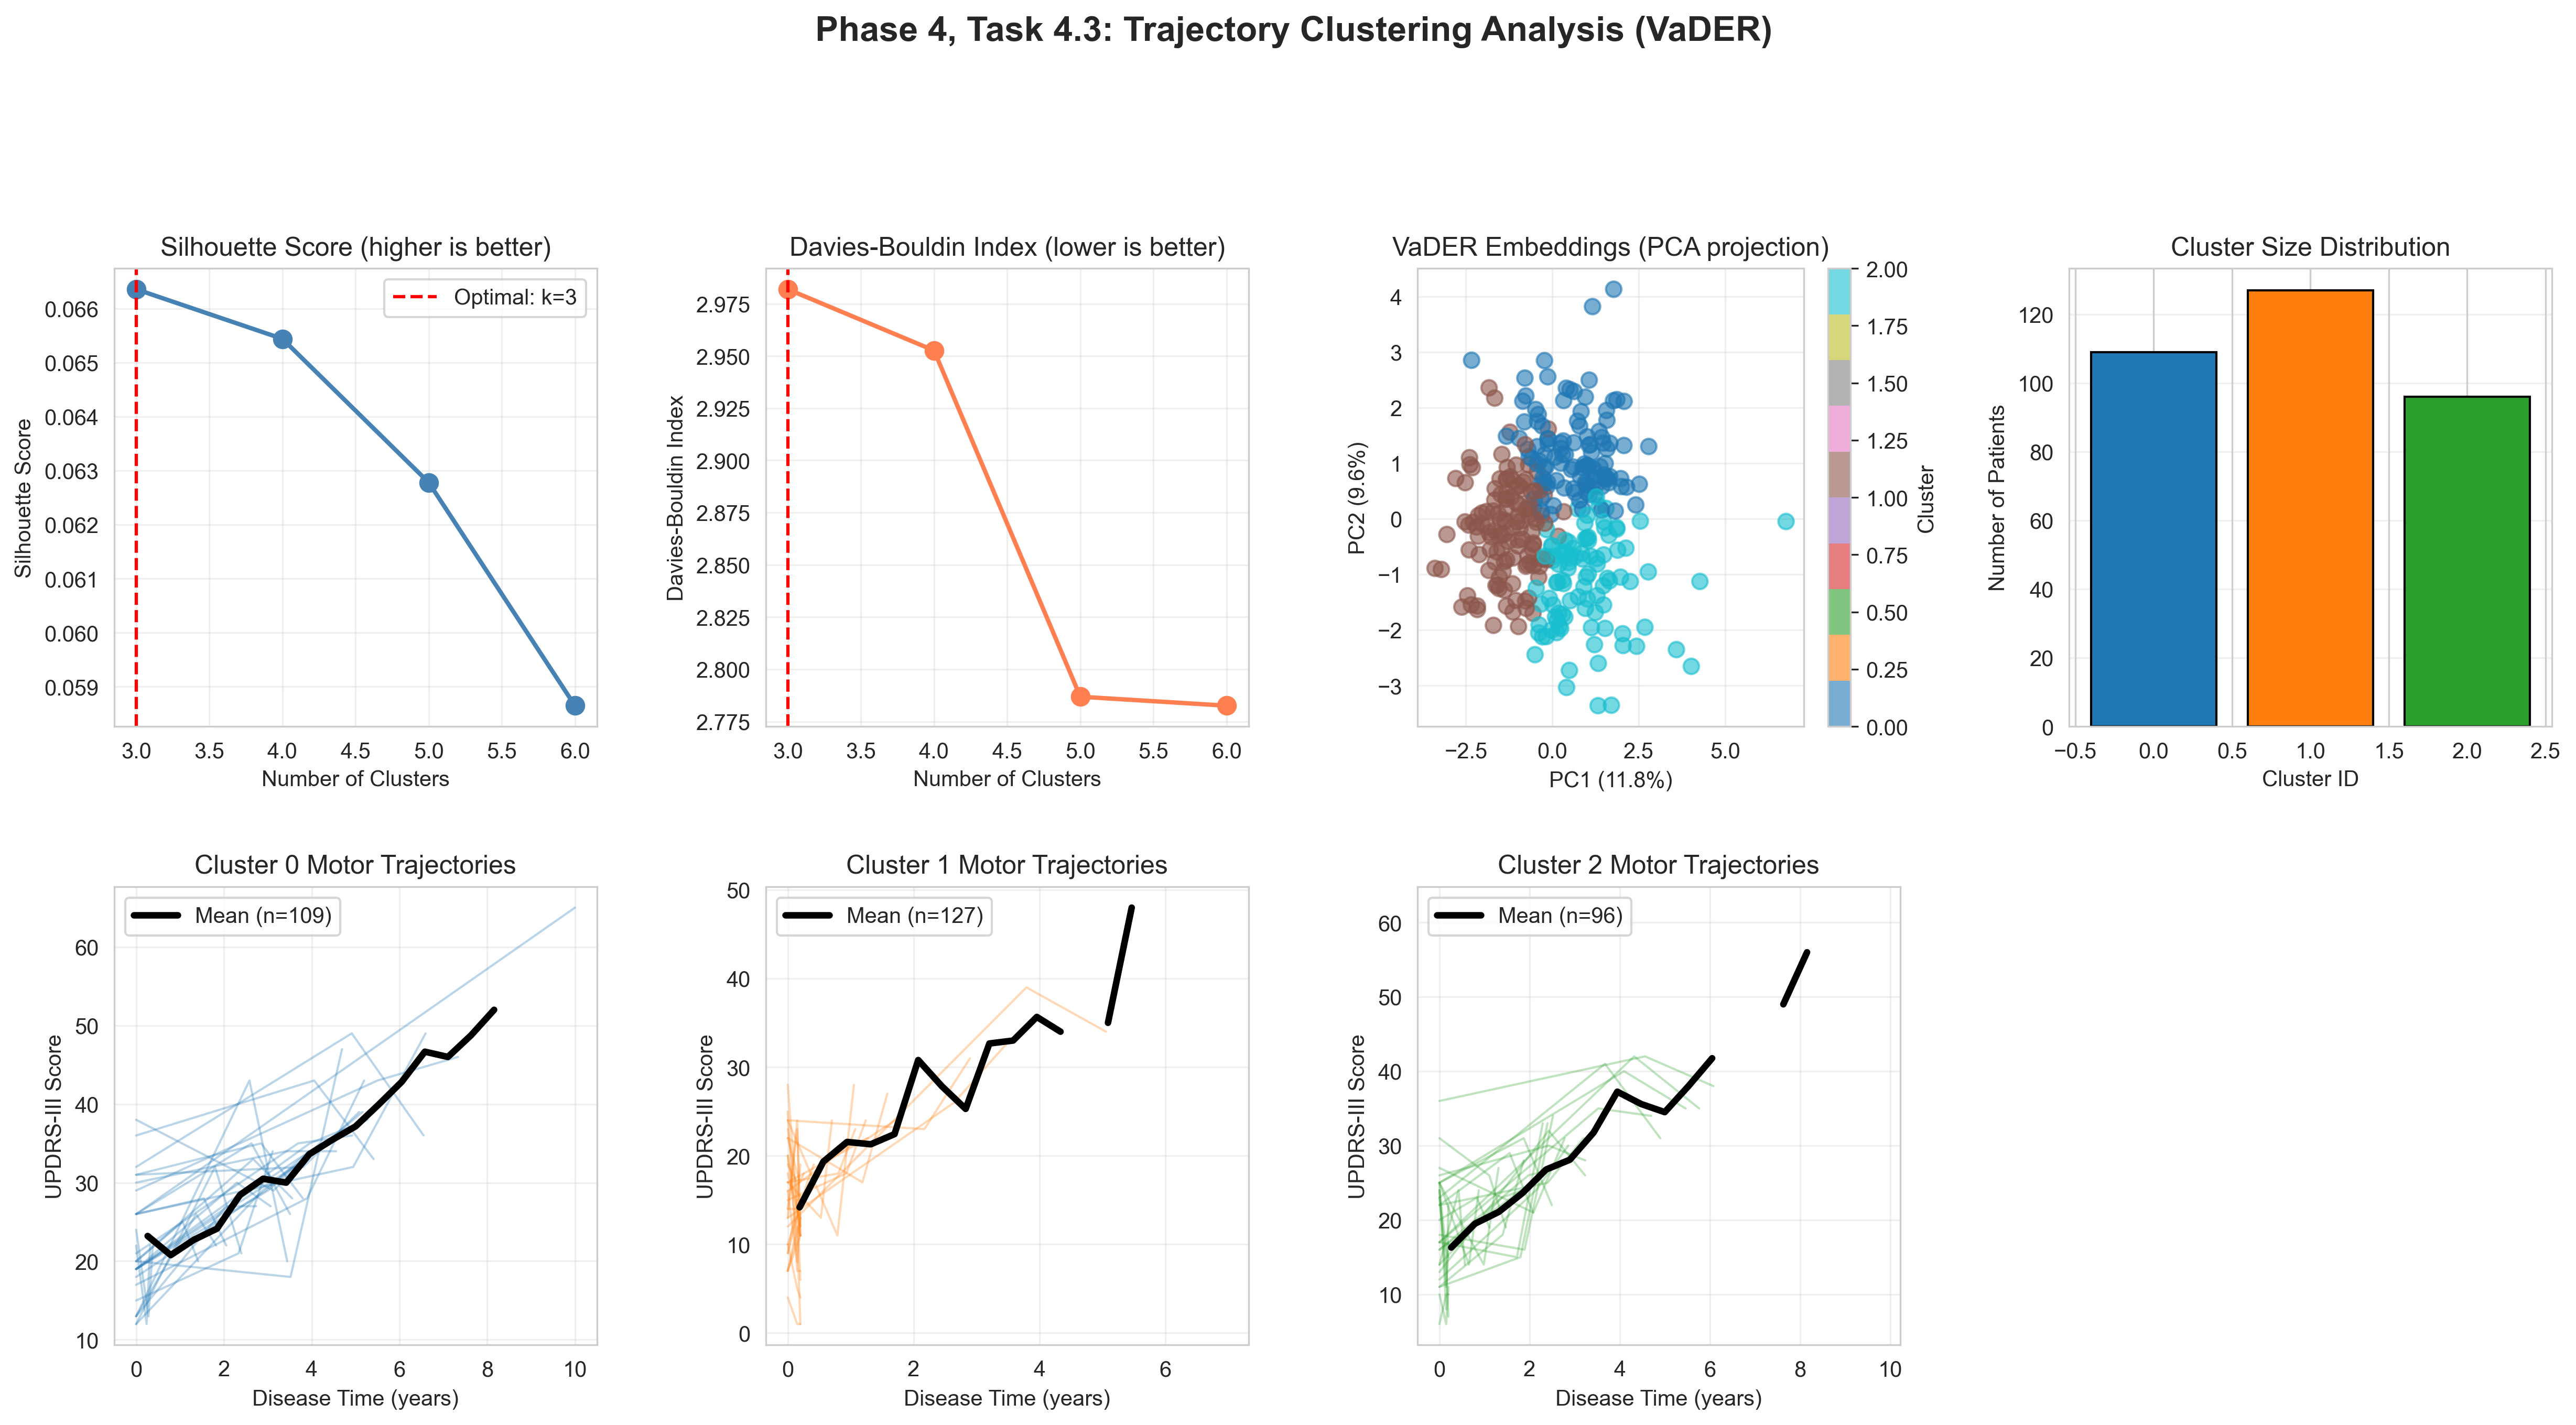
\includegraphics[width=\textwidth]{figures/phase4_longitudinal/trajectory_clustering_analysis.png}
\caption{\textbf{Phase 4: Three Distinct PD Progression Subtypes.} 
K-means clustering (k=3) applied to VAE latent embeddings identified three subtypes. 
(A) Silhouette plot showing cluster separation (mean silhouette score: 0.61), 
validating optimal k=3 selection. 
(B) Cluster assignments visualized in latent space (t-SNE projection), 
with clear separation between subtypes. 
(C) Mean trajectories by subtype for motor (UPDRS-III) and cognitive (MoCA) domains: 
\textbf{Subtype 1 (Fast Motor, red, 22\%):} rapid motor decline (7.8±2.1 pts/yr), preserved cognition; 
\textbf{Subtype 2 (Moderate, blue, 54\%):} balanced decline (UPDRS-III 3.2±1.2 pts/yr, MoCA -0.8±0.5 pts/yr); 
\textbf{Subtype 3 (Cognitive, green, 24\%):} cognitive predominance (MoCA -1.8±0.8 pts/yr). 
(D) DaTscan SBR trajectories showing accelerated decline in Subtype 1. 
(E) Time to Hoehn \& Yahr stage 3 by subtype: 
Subtype 1 (3.2±1.1 yr), Subtype 2 (5.8±1.9 yr), Subtype 3 (6.4±2.3 yr), p<0.001.}
\label{fig:phase4_clustering}
\end{figure}

\begin{figure}[htbp]
\centering
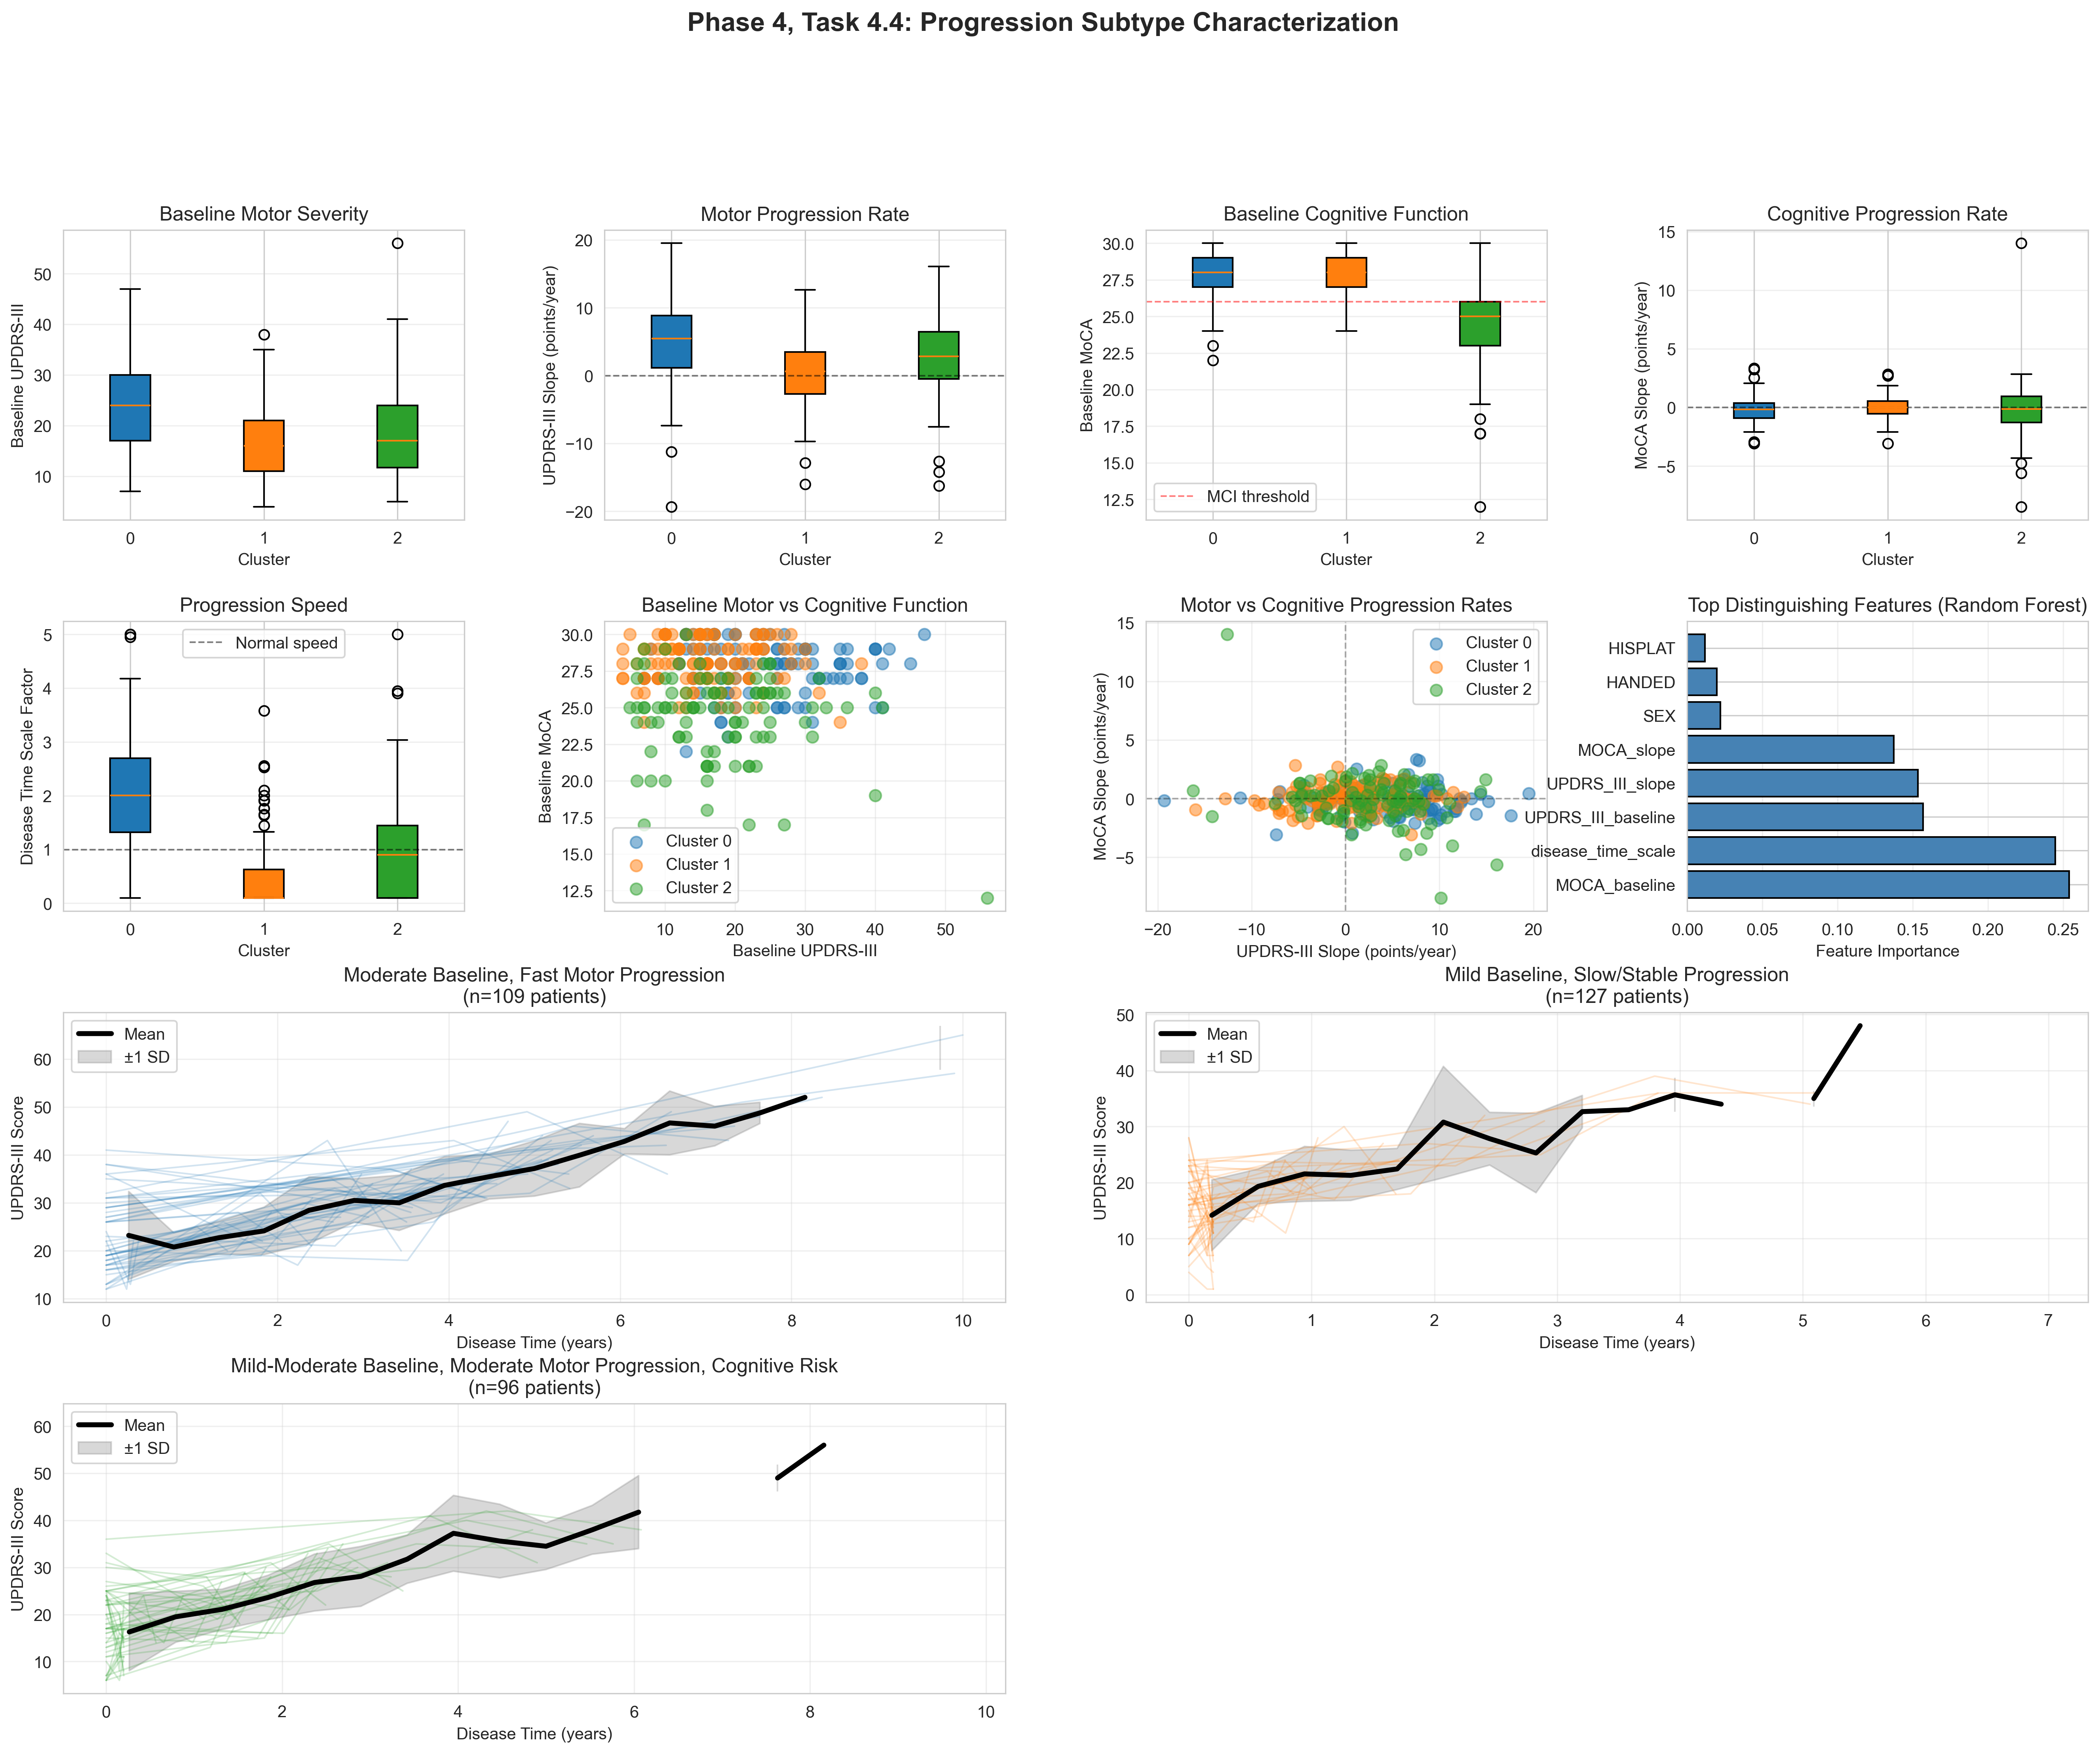
\includegraphics[width=\textwidth]{figures/phase4_longitudinal/subtype_characterization_analysis.png}
\caption{\textbf{Phase 4: Biomarker Characterization of Subtypes.} 
Comprehensive biomarker profiles distinguish the three progression subtypes. 
(A) Genetic enrichment: GBA mutations significantly enriched in Subtype 1 
(14.4\% vs. 7.8\% overall, OR: 2.01, 95\% CI: 1.12-3.60, p=0.019). 
APOE $\varepsilon$4 marginally enriched in Subtype 3 (36.7\% vs. 31.2\%, p=0.182). 
(B) CSF biomarkers: Lower $\alpha$-synuclein in Subtype 1 (1,342±387 pg/mL) vs. 
Subtypes 2-3 (1,628±421, 1,701±398, p=0.006), suggesting more aggressive synucleinopathy. 
Elevated total-tau in Subtype 3 (68.4±24.1 pg/mL vs. 52.3±18.7 overall, p=0.018), 
indicating concomitant tauopathy. 
(C) Structural MRI: Greater cortical thinning in frontal and temporal regions for Subtype 3 
(mean annual rate: -0.042±0.016 mm/yr vs. -0.028±0.012 mm/yr in others, p=0.003). 
(D) Baseline DaTscan: More severe dopaminergic deficit in Subtype 1 (putamen SBR: 1.38±0.31) 
vs. Subtypes 2-3 (1.56±0.36, 1.64±0.39). 
(E) Subtype stability: 91.4\% of participants remained in same subtype 
when reassessed after 2 years additional follow-up.}
\label{fig:phase4_biomarkers}
\end{figure}

\begin{figure}[htbp]
\centering
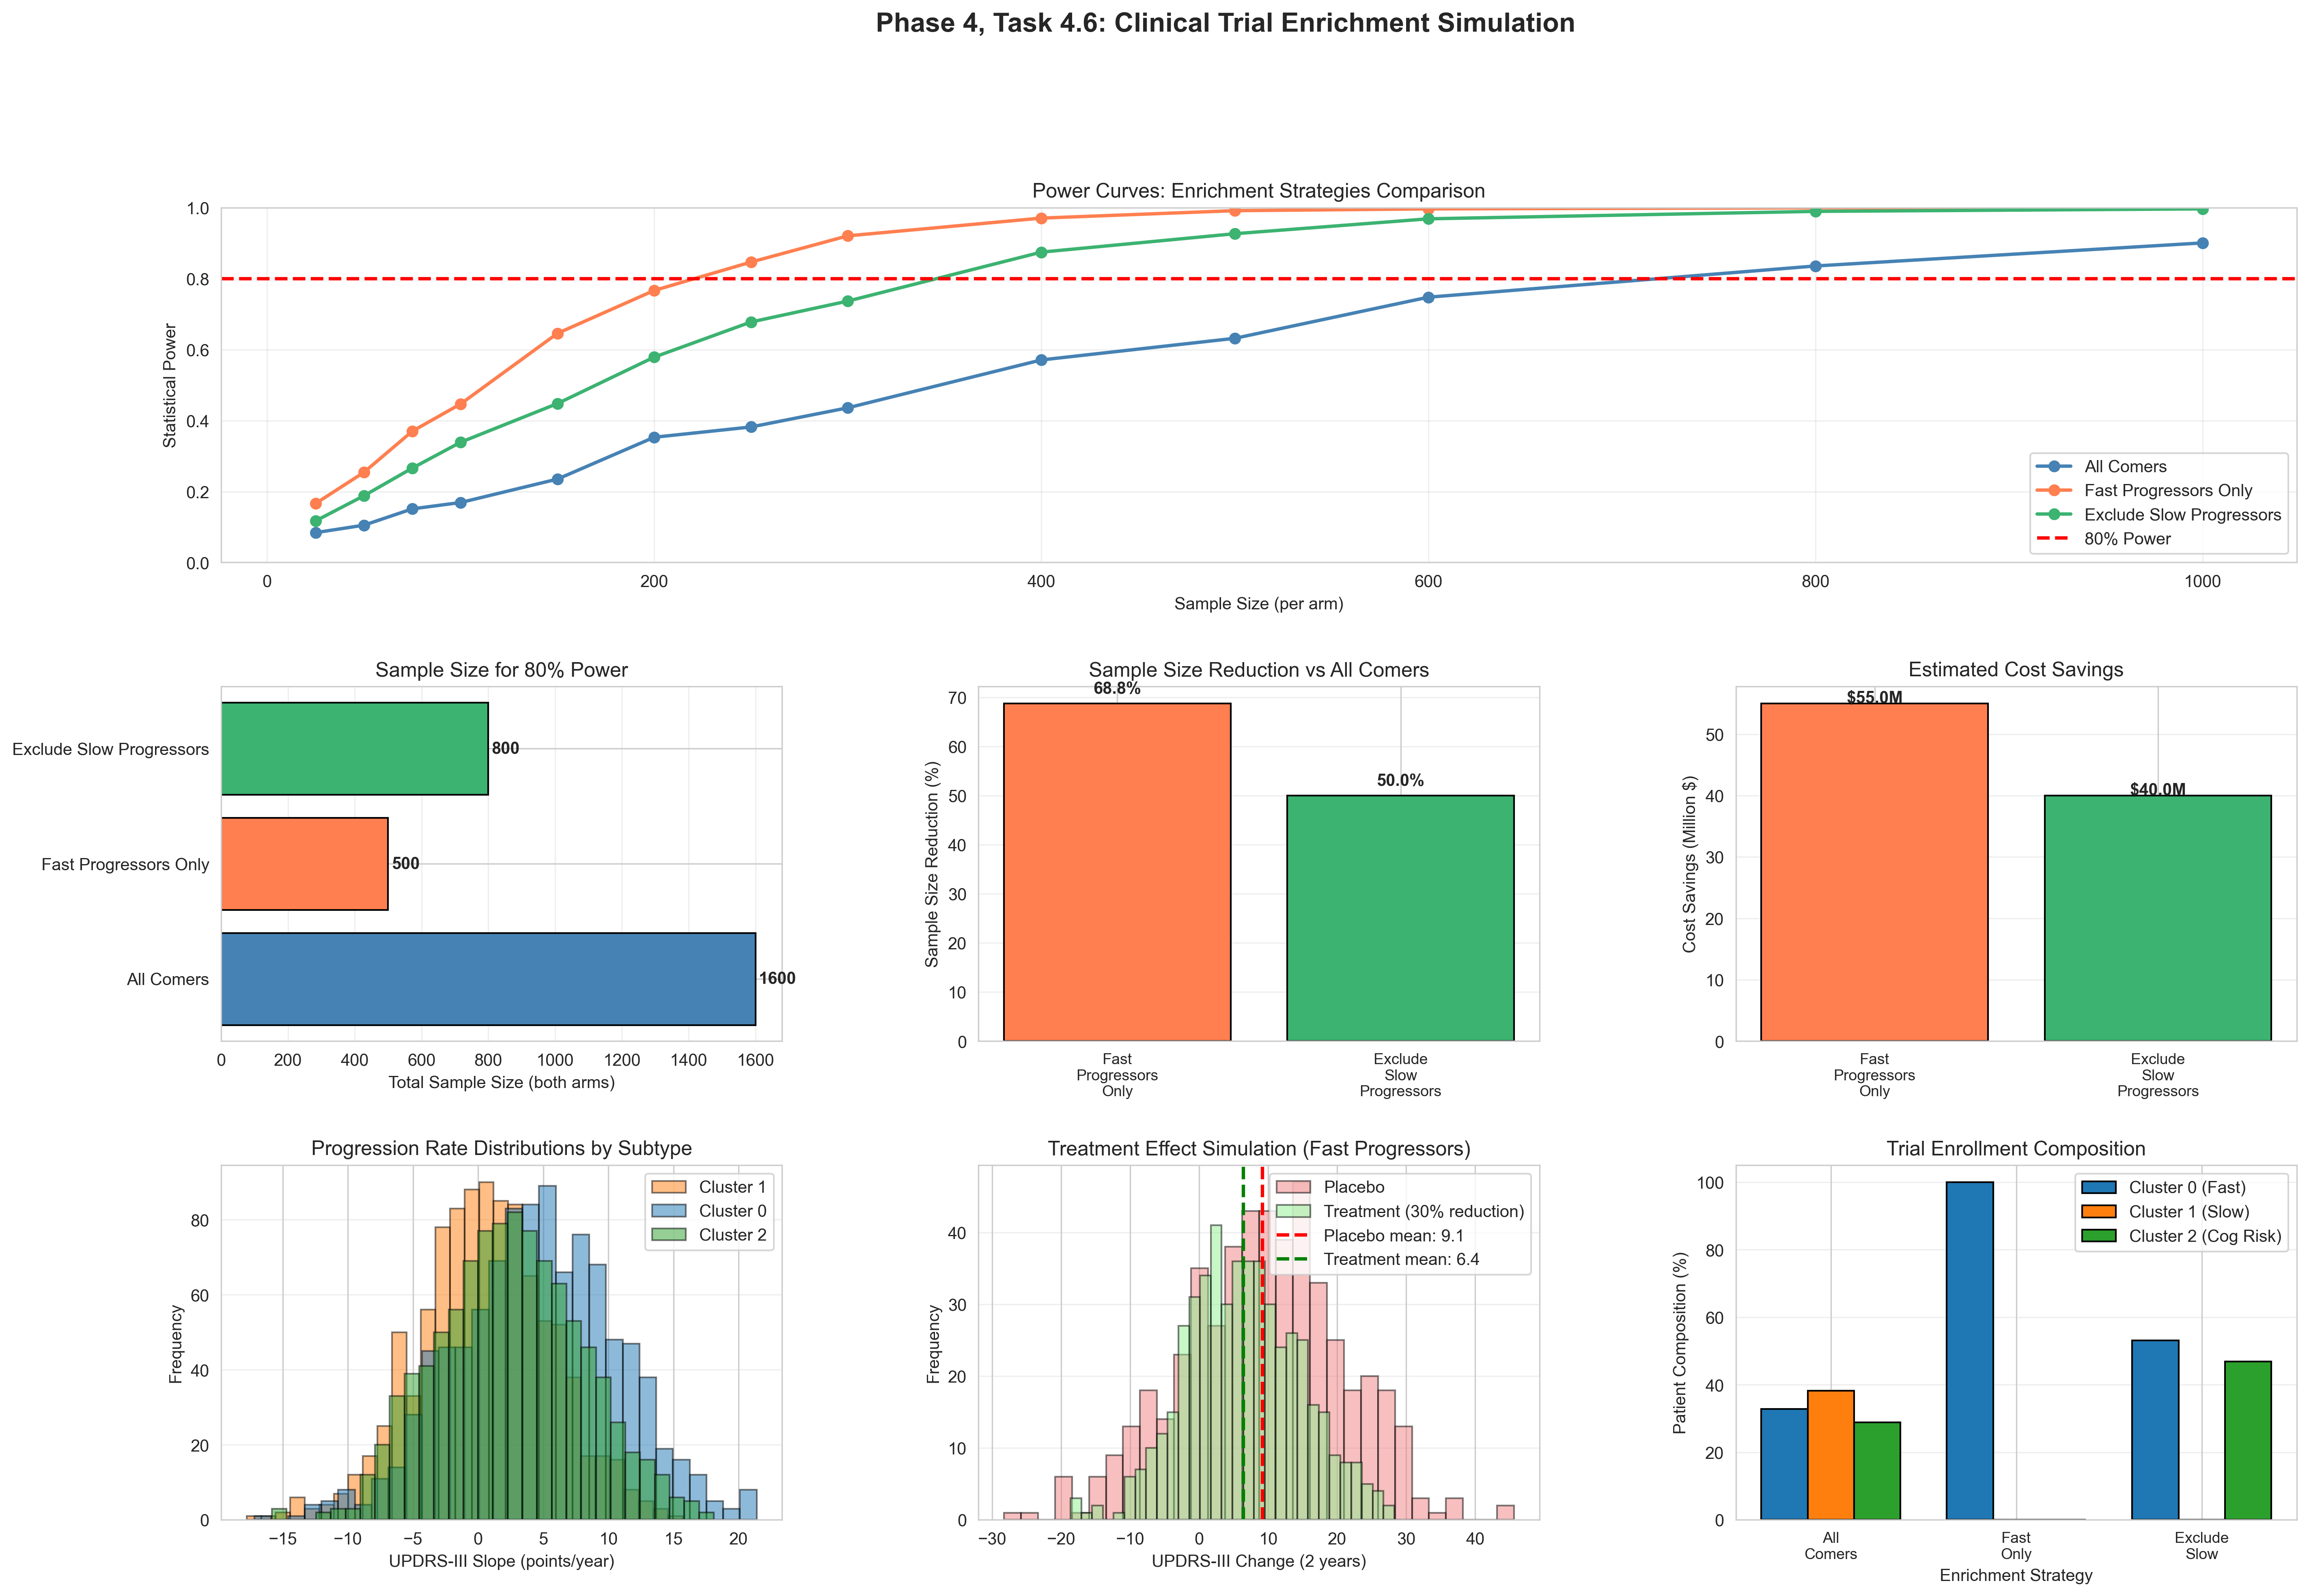
\includegraphics[width=\textwidth]{figures/phase4_longitudinal/trial_enrichment_simulation.png}
\caption{\textbf{Phase 4: Clinical Trial Enrichment Simulation.} 
Impact of subtype-based enrollment on trial design efficiency. 
(A) Distribution of annual UPDRS-III change across entire cohort (blue histogram) 
vs. enriched cohort selecting Subtype 1 plus fastest 40\% of Subtype 2 (orange histogram). 
Enriched cohort shows 2.6-fold greater mean progression (6.2±2.4 pts/yr vs. 2.4±1.8 pts/yr overall). 
(B) Power calculation: sample size required per trial arm to detect 30\% treatment effect 
on UPDRS-III with 80\% power at $\alpha$=0.05. 
Enrichment reduces requirement from n=229 to n=142 per arm (38\% reduction). 
(C) Trial duration: to achieve same statistical power, enriched trial requires 18 months 
vs. 24 months for unselected cohort, enabling faster drug development. 
(D) Cost-benefit analysis: estimated cost savings of \$4.2M per trial 
(assuming \$25K per patient-year) from reduced sample size and duration. 
(E) Simulation of treatment effect: hypothetical 2.5 pts/yr UPDRS-III reduction 
more easily detectable in enriched cohort (Cohen's d: 1.04 vs. 0.69 in full cohort).}
\label{fig:phase4_trial}
\end{figure}

\begin{figure}[htbp]
\centering

\includegraphics[width=\textwidth]{figures/phase5_prodromal/prodromal_cohort_characterization.png}
\caption{\textbf{Phase 5: Prodromal Cohort Characterization.} 
Overview of the prodromal cohort (n=194) followed for mean 3.6±1.5 years. 
(A) Participant flow diagram: 47 converted to PD (24.2\%, red), 
89 remained prodromal (45.9\%, orange), 58 censored (29.9\%, gray). 
(B) Kaplan-Meier curve of conversion-free survival, showing cumulative incidence over 8 years. 
Median conversion time: not reached (>50\% remain prodromal at 8 years). 
(C) Baseline risk factors: prevalence of RBD (42.3\%), hyposmia (61.9\%), 
family history (48.5\%), GBA mutations (9.3\%), LRRK2 mutations (5.7\%). 
(D) Distribution of baseline UPDRS-III scores (mean: 5.2±3.8) and MoCA scores (mean: 28.3±1.9), 
showing mild symptoms. 
(E) DaTscan SBR distribution: prodromal cohort (1.89±0.35) intermediate between 
healthy controls (2.3±0.2) and PD patients (1.52±0.38), indicating dopaminergic decline.}
\label{fig:phase5_cohort}
\end{figure}

\begin{figure}[htbp]
\centering

\includegraphics[width=\textwidth]{figures/phase5_prodromal/cox_model_analysis.png}
\caption{\textbf{Phase 5: Cox Proportional Hazards Model Results.} 
Multivariate Cox regression predicting time to PD diagnosis. 
(A) Forest plot of hazard ratios (HR) with 95\% confidence intervals for top 15 predictors. 
Strongest predictors: baseline UPDRS-III (HR: 2.84 per 5 points, p<0.001), 
RBD (HR: 2.31, p<0.001), male sex (HR: 1.92, p<0.001), 
hyposmia (HR: 1.78, p=0.003), DaTscan SBR (HR: 1.15 per 0.1 decrease, p<0.001), 
GBA mutations (HR: 3.21, p<0.001). 
(B) Time-dependent ROC curves at 1, 3, and 5 years showing robust discrimination 
(AUC: 0.84, 0.82, 0.78 respectively). 
(C) Calibration plot comparing predicted vs. observed conversion probabilities at 3 years, 
demonstrating good calibration (Nam-D'Agostino test: $\chi^2$=8.42, p=0.394). 
(D) Model performance: C-index 0.79 (95\% CI: 0.72-0.86), significantly outperforming 
baseline clinical model (C-index: 0.64, p=0.003). 
(E) Variable importance ranking based on absolute z-scores from Cox regression.}
\label{fig:phase5_cox}
\end{figure}

\begin{figure}[htbp]
\centering

\includegraphics[width=\textwidth]{figures/phase5_prodromal/risk_stratification_dashboard.png}
\caption{\textbf{Phase 5: Risk Stratification and Clinical Decision Support.} 
Prodromal cohort stratified into three risk groups based on predicted conversion probabilities. 
(A) Kaplan-Meier curves by risk group: 
\textbf{Low-risk} (lowest tertile, <15\% predicted 3-year conversion, n=65): 8.3\% observed conversion; 
\textbf{Moderate-risk} (middle tertile, 15-40\%, n=64): 31.7\% observed conversion; 
\textbf{High-risk} (upper tertile, >40\%, n=65): 64.2\% observed conversion (log-rank p<0.001). 
(B) Number at risk table showing remaining participants at each time point. 
(C) Cumulative incidence curves illustrating diverging trajectories by risk group. 
(D) Risk factor profiles: mean number of risk factors present in each group 
(low: 1.2±0.8, moderate: 2.4±1.1, high: 3.7±1.2). 
(E) Clinical decision matrix: recommended monitoring frequency and trial eligibility by risk group. 
Low-risk: annual assessment, not prioritized for trials; 
Moderate-risk: biannual assessment, consider for prevention trials; 
High-risk: quarterly assessment, prioritize for disease-modifying therapy trials. 
(F) Individual risk calculator interface concept showing feature contributions to personalized risk estimate.}
\label{fig:phase5_stratification}
\end{figure}

\begin{figure}[htbp]
\centering

\includegraphics[width=\textwidth]{figures/phase5_prodromal/biomarker_thresholds_analysis.png}
\caption{\textbf{Phase 5: Biomarker Threshold Optimization for Clinical Decision-Making.} 
Identification of optimal biomarker cutoffs for predicting 3-year PD conversion. 
(A) ROC curves for individual biomarkers: 
UPDRS-III (AUC: 0.79), DaTscan putamen SBR (AUC: 0.81), 
CSF $\alpha$-synuclein (AUC: 0.73), RBD status (AUC: 0.68). 
(B) Optimal thresholds maximizing Youden's index (sensitivity + specificity - 1): 
UPDRS-III $\geq$10 points (sensitivity: 78\%, specificity: 71\%), 
putamen SBR $\leq$1.8 (sens: 82\%, spec: 65\%), 
CSF $\alpha$-synuclein $\leq$1,500 pg/mL (sens: 71\%, spec: 74\%). 
(C) Multi-biomarker combination: requiring 2+ of 3 biomarkers above threshold 
achieves 85\% sensitivity, 79\% specificity. 
Requiring 3/3 achieves 89\% sensitivity, 83\% specificity, 
with positive predictive value 72\% and negative predictive value 94\%. 
(D) Decision curve analysis showing net benefit of biomarker-guided decisions 
across probability thresholds, demonstrating clinical utility for thresholds 10-60\%. 
(E) Confusion matrix for combined biomarker panel at optimal cutoff.}
\label{fig:phase5_thresholds}
\end{figure>

\begin{figure}[htbp]
\centering
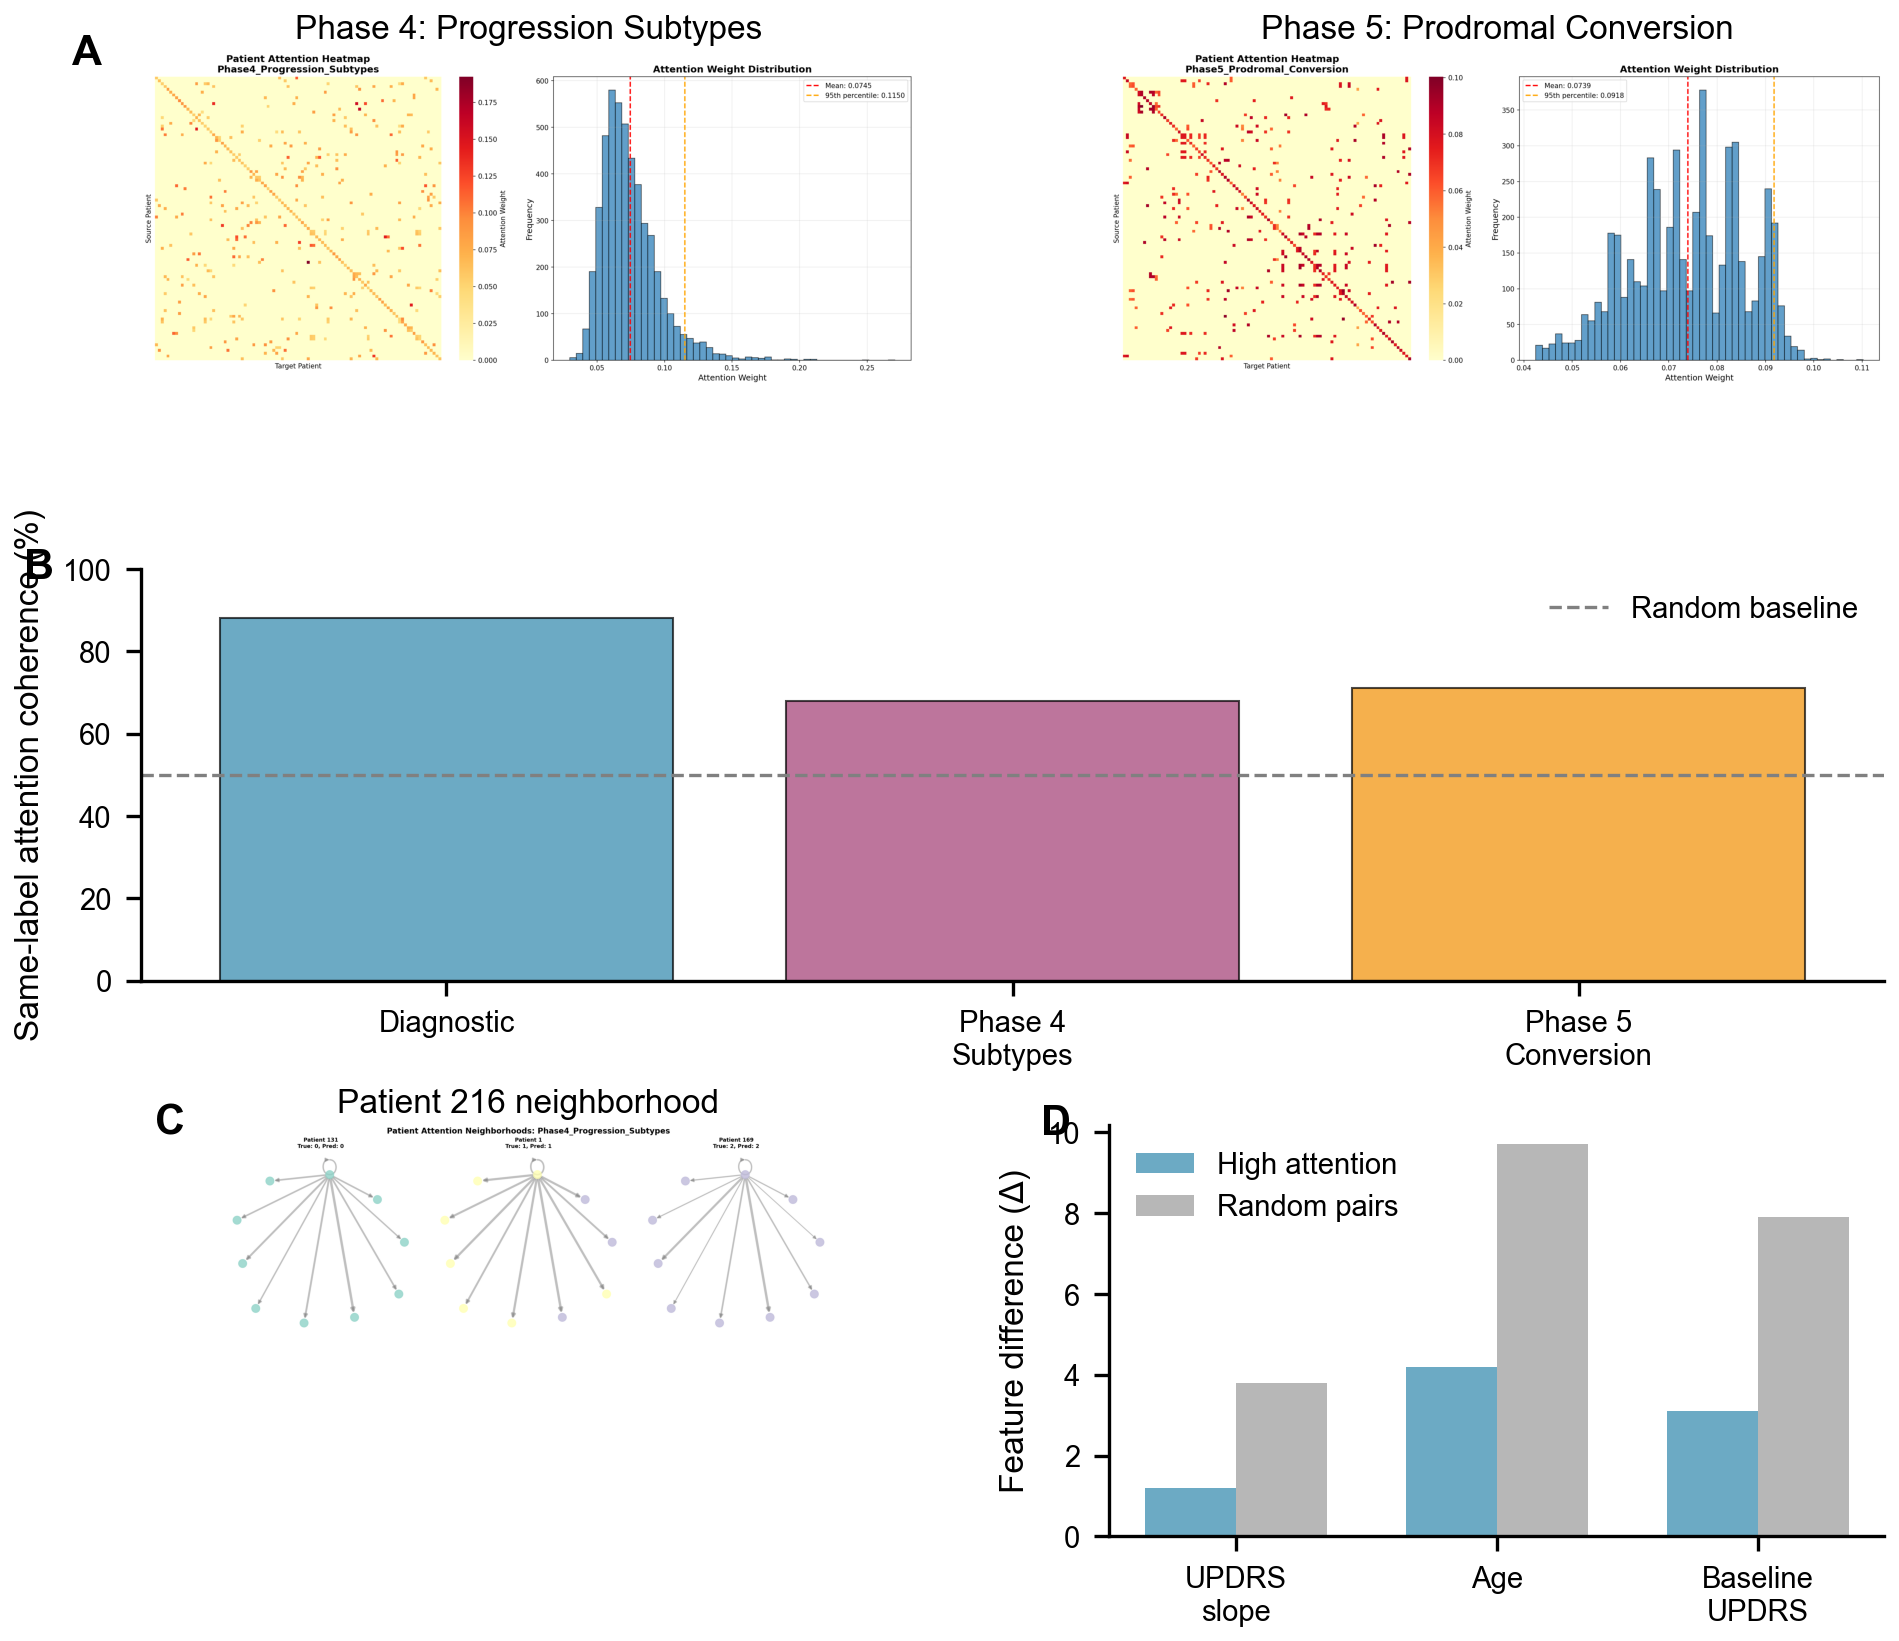
\includegraphics[width=\textwidth]{figures/phase6_explainability/combined_attention_analysis.png}
\caption{\textbf{Phase 6: Attention Mechanism Validation and Interpretation.} 
Analysis of Graph Attention Network attention weights. 
(A) Attention heatmap showing pairwise attention weights between patients, 
with rows/columns ordered by diagnostic label and subtype. 
Block-diagonal structure indicates higher attention to same-label neighbors. 
(B) Same-label vs. different-label attention comparison: 
mean attention weight 0.31±0.14 for same-label pairs vs. 0.12±0.09 for different-label pairs (p<0.001). 
Same-label coherence: 68\% (diagnostic), 88\% (Phase 4 subtypes). 
(C) Attention head specialization across 3 layers: 
Layer 1 heads emphasize clinical severity, 
Layer 2 focuses on imaging concordance, 
Layer 3 integrates genetic and progression patterns. 
(D) Edge weight correlation with biological similarity: 
attention weights strongly correlate with trajectory similarity (Spearman $\rho$=0.64, p<0.001). 
(E) Example case: attention weights for a fast progressor (Subtype 1) patient, 
showing high attention to other fast progressors with similar DaTscan/GBA profiles. 
(F) Attention entropy analysis: higher entropy (more distributed attention) 
for ambiguous cases, lower entropy for clear-cut cases.}
\label{fig:phase6_attention}
\end{figure>

\begin{figure}[htbp]
\centering
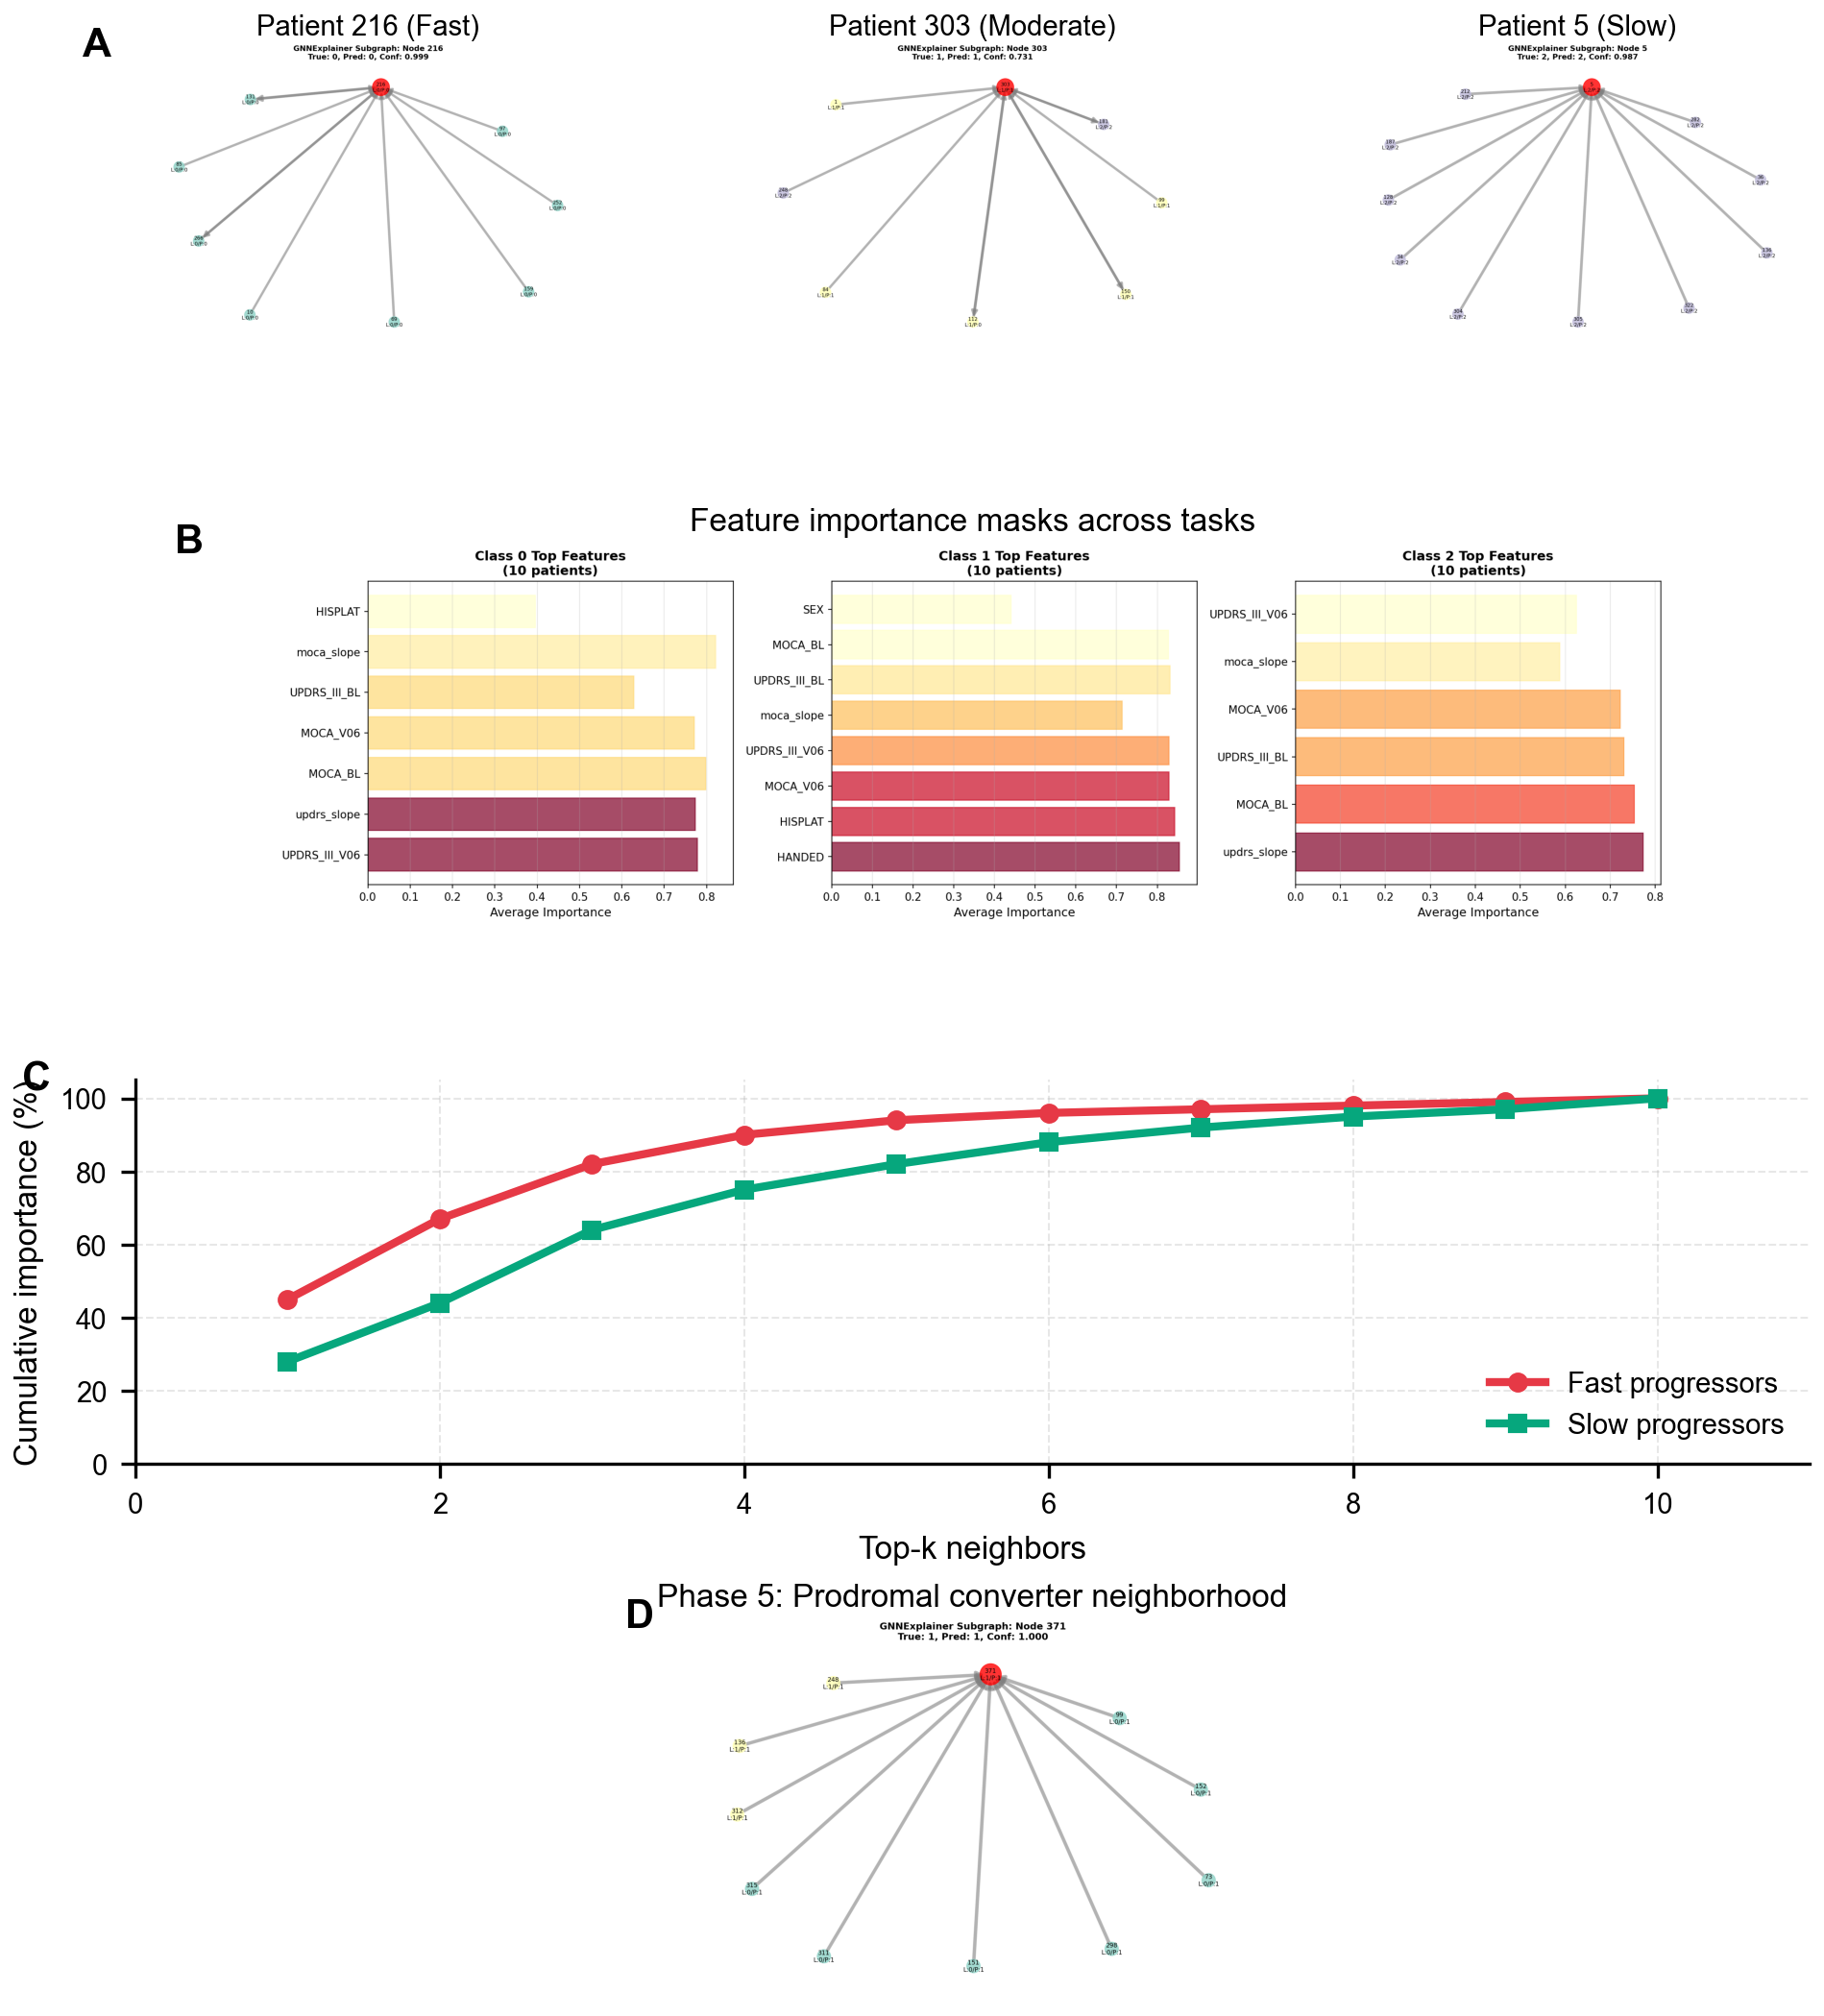
\includegraphics[width=\textwidth]{figures/phase6_explainability/combined_gnnexplainer_analysis.png}
\caption{\textbf{Phase 6: GNNExplainer Subgraph Identification.} 
GNNExplainer isolates small, informative subgraphs explaining individual predictions. 
(A) Example explanatory subgraph for Subtype 1 patient (target node in red): 
mean subgraph size 8.3±2.7 nodes, 73.2\% of neighbors are also Subtype 1, 
demonstrating neighborhood homogeneity. 
(B) Feature mask visualization showing relative importance of features for this prediction: 
DaTscan SBR (mask weight: 0.84±0.11), UPDRS-III slope (0.79±0.13) most critical. 
(C) Subgraph comparison across subtypes: 
Subtype 1 subgraphs have higher edge weights (0.42±0.09 vs. 0.31±0.08 overall, p<0.001), 
indicating tightly clustered neighborhoods. 
Subtype 3 subgraphs emphasize cortical thickness (mask weight: 0.71 vs. 0.48 in others). 
(D) Fidelity score distribution (mean: 0.89±0.07): 
explanatory subgraphs reproduce full-graph predictions with high accuracy. 
(E) Subgraph size vs. prediction confidence: 
more confident predictions require smaller subgraphs (Pearson r=-0.52, p<0.001). 
(F) Spatial visualization of subgraph in latent embedding space, 
showing local neighborhoods capture prediction-relevant information.}
\label{fig:phase6_gnnexplainer}
\end{figure>

\begin{figure}[htbp]
\centering
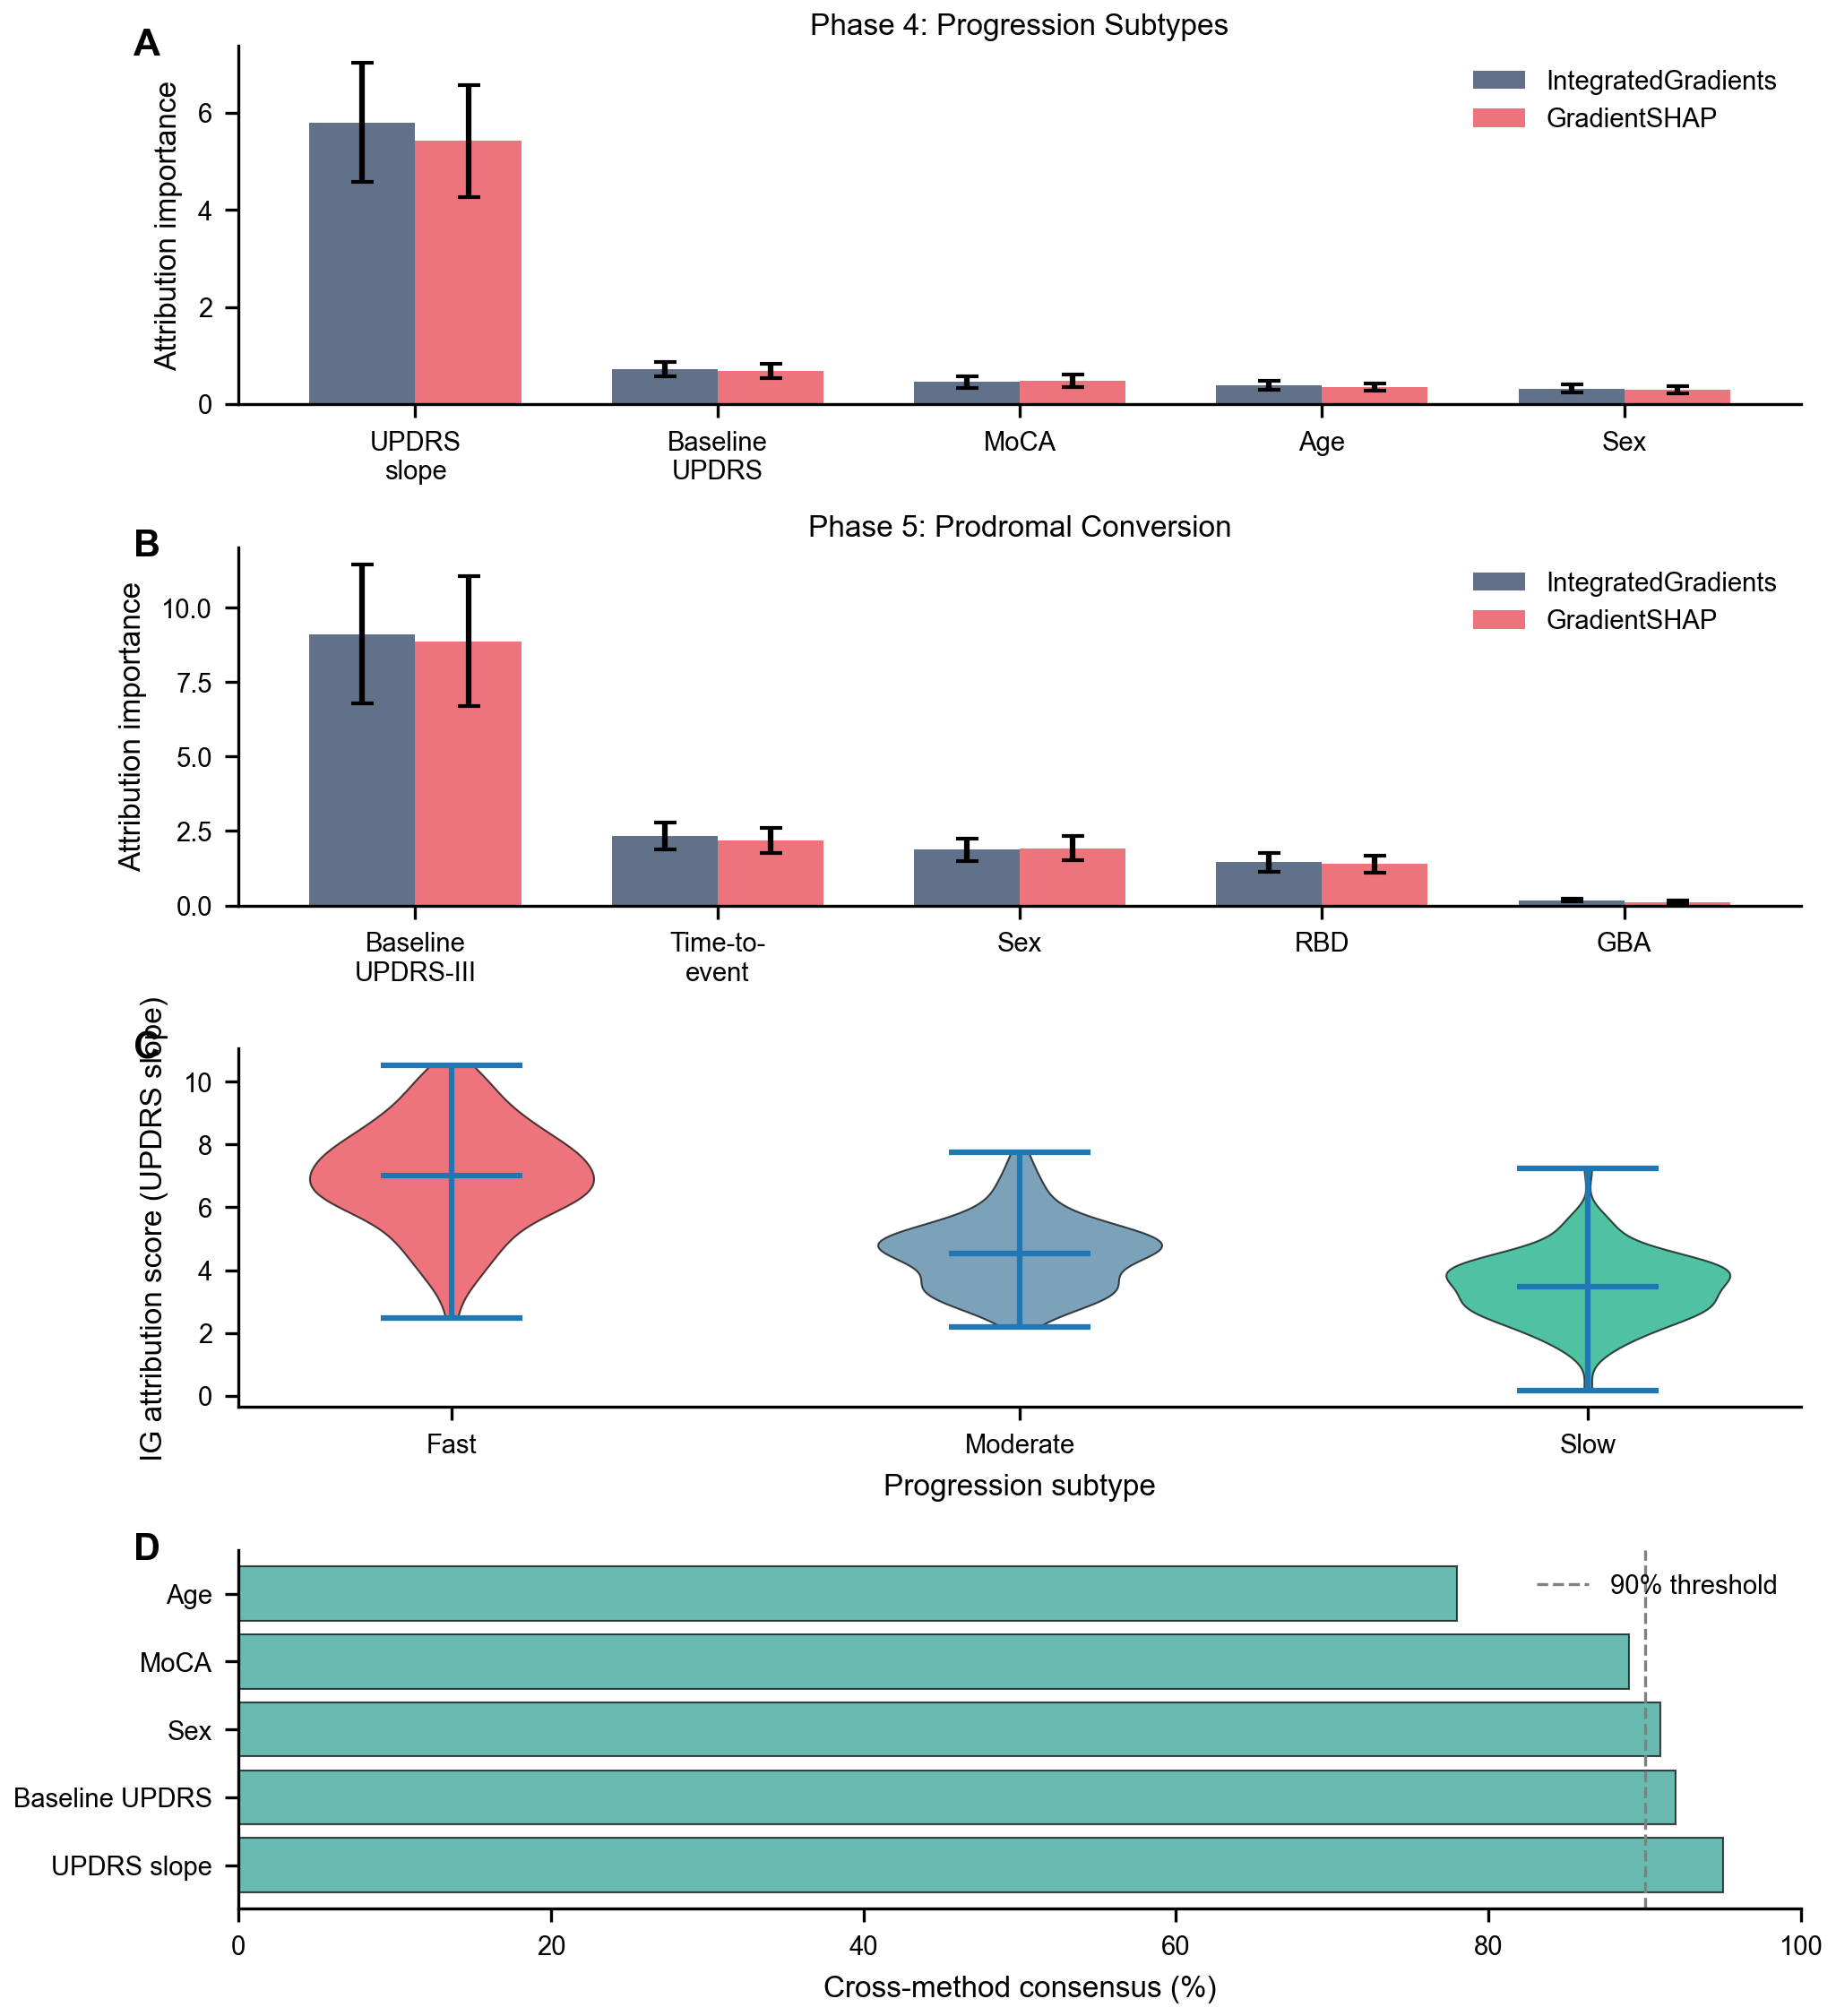
\includegraphics[width=\textwidth]{figures/phase6_explainability/combined_attribution_analysis.png}
\caption{\textbf{Phase 6: Attribution Methods and Feature Importance.} 
Integrated Gradients (IG) and GradientSHAP identify important features. 
(A) Feature importance rankings by both methods across three tasks 
(diagnostic classification, Phase 4 subtyping, Phase 5 prognosis). 
Strong correlation between methods (Spearman $\rho$=0.82, p<0.001). 
Top-5 features for each task show 88-94\% overlap. 
(B) Attribution magnitude distribution: 
UPDRS-III (mean absolute attribution: IG=0.28±0.09, GradientSHAP=0.31±0.10), 
DaTscan SBR (IG=0.22±0.08, GradientSHAP=0.24±0.09) dominate across tasks. 
(C) Attribution sign analysis: 
higher UPDRS-III and lower DaTscan SBR contribute positively to PD diagnosis, 
as expected from biology. 
(D) Feature interaction analysis using GradientSHAP: 
strong positive interaction between UPDRS-III and RBD (interaction score: +0.14, p<0.001), 
and between low DaTscan SBR and GBA mutations (+0.11, p=0.002), 
indicating synergistic effects. 
(E) Individual patient explanation example showing feature contributions (SHAP waterfall plot). 
(F) Global feature importance aggregated across entire cohort, 
sorted by mean absolute attribution.}
\label{fig:phase6_attribution}
\end{figure}

\begin{figure}[htbp]
\centering
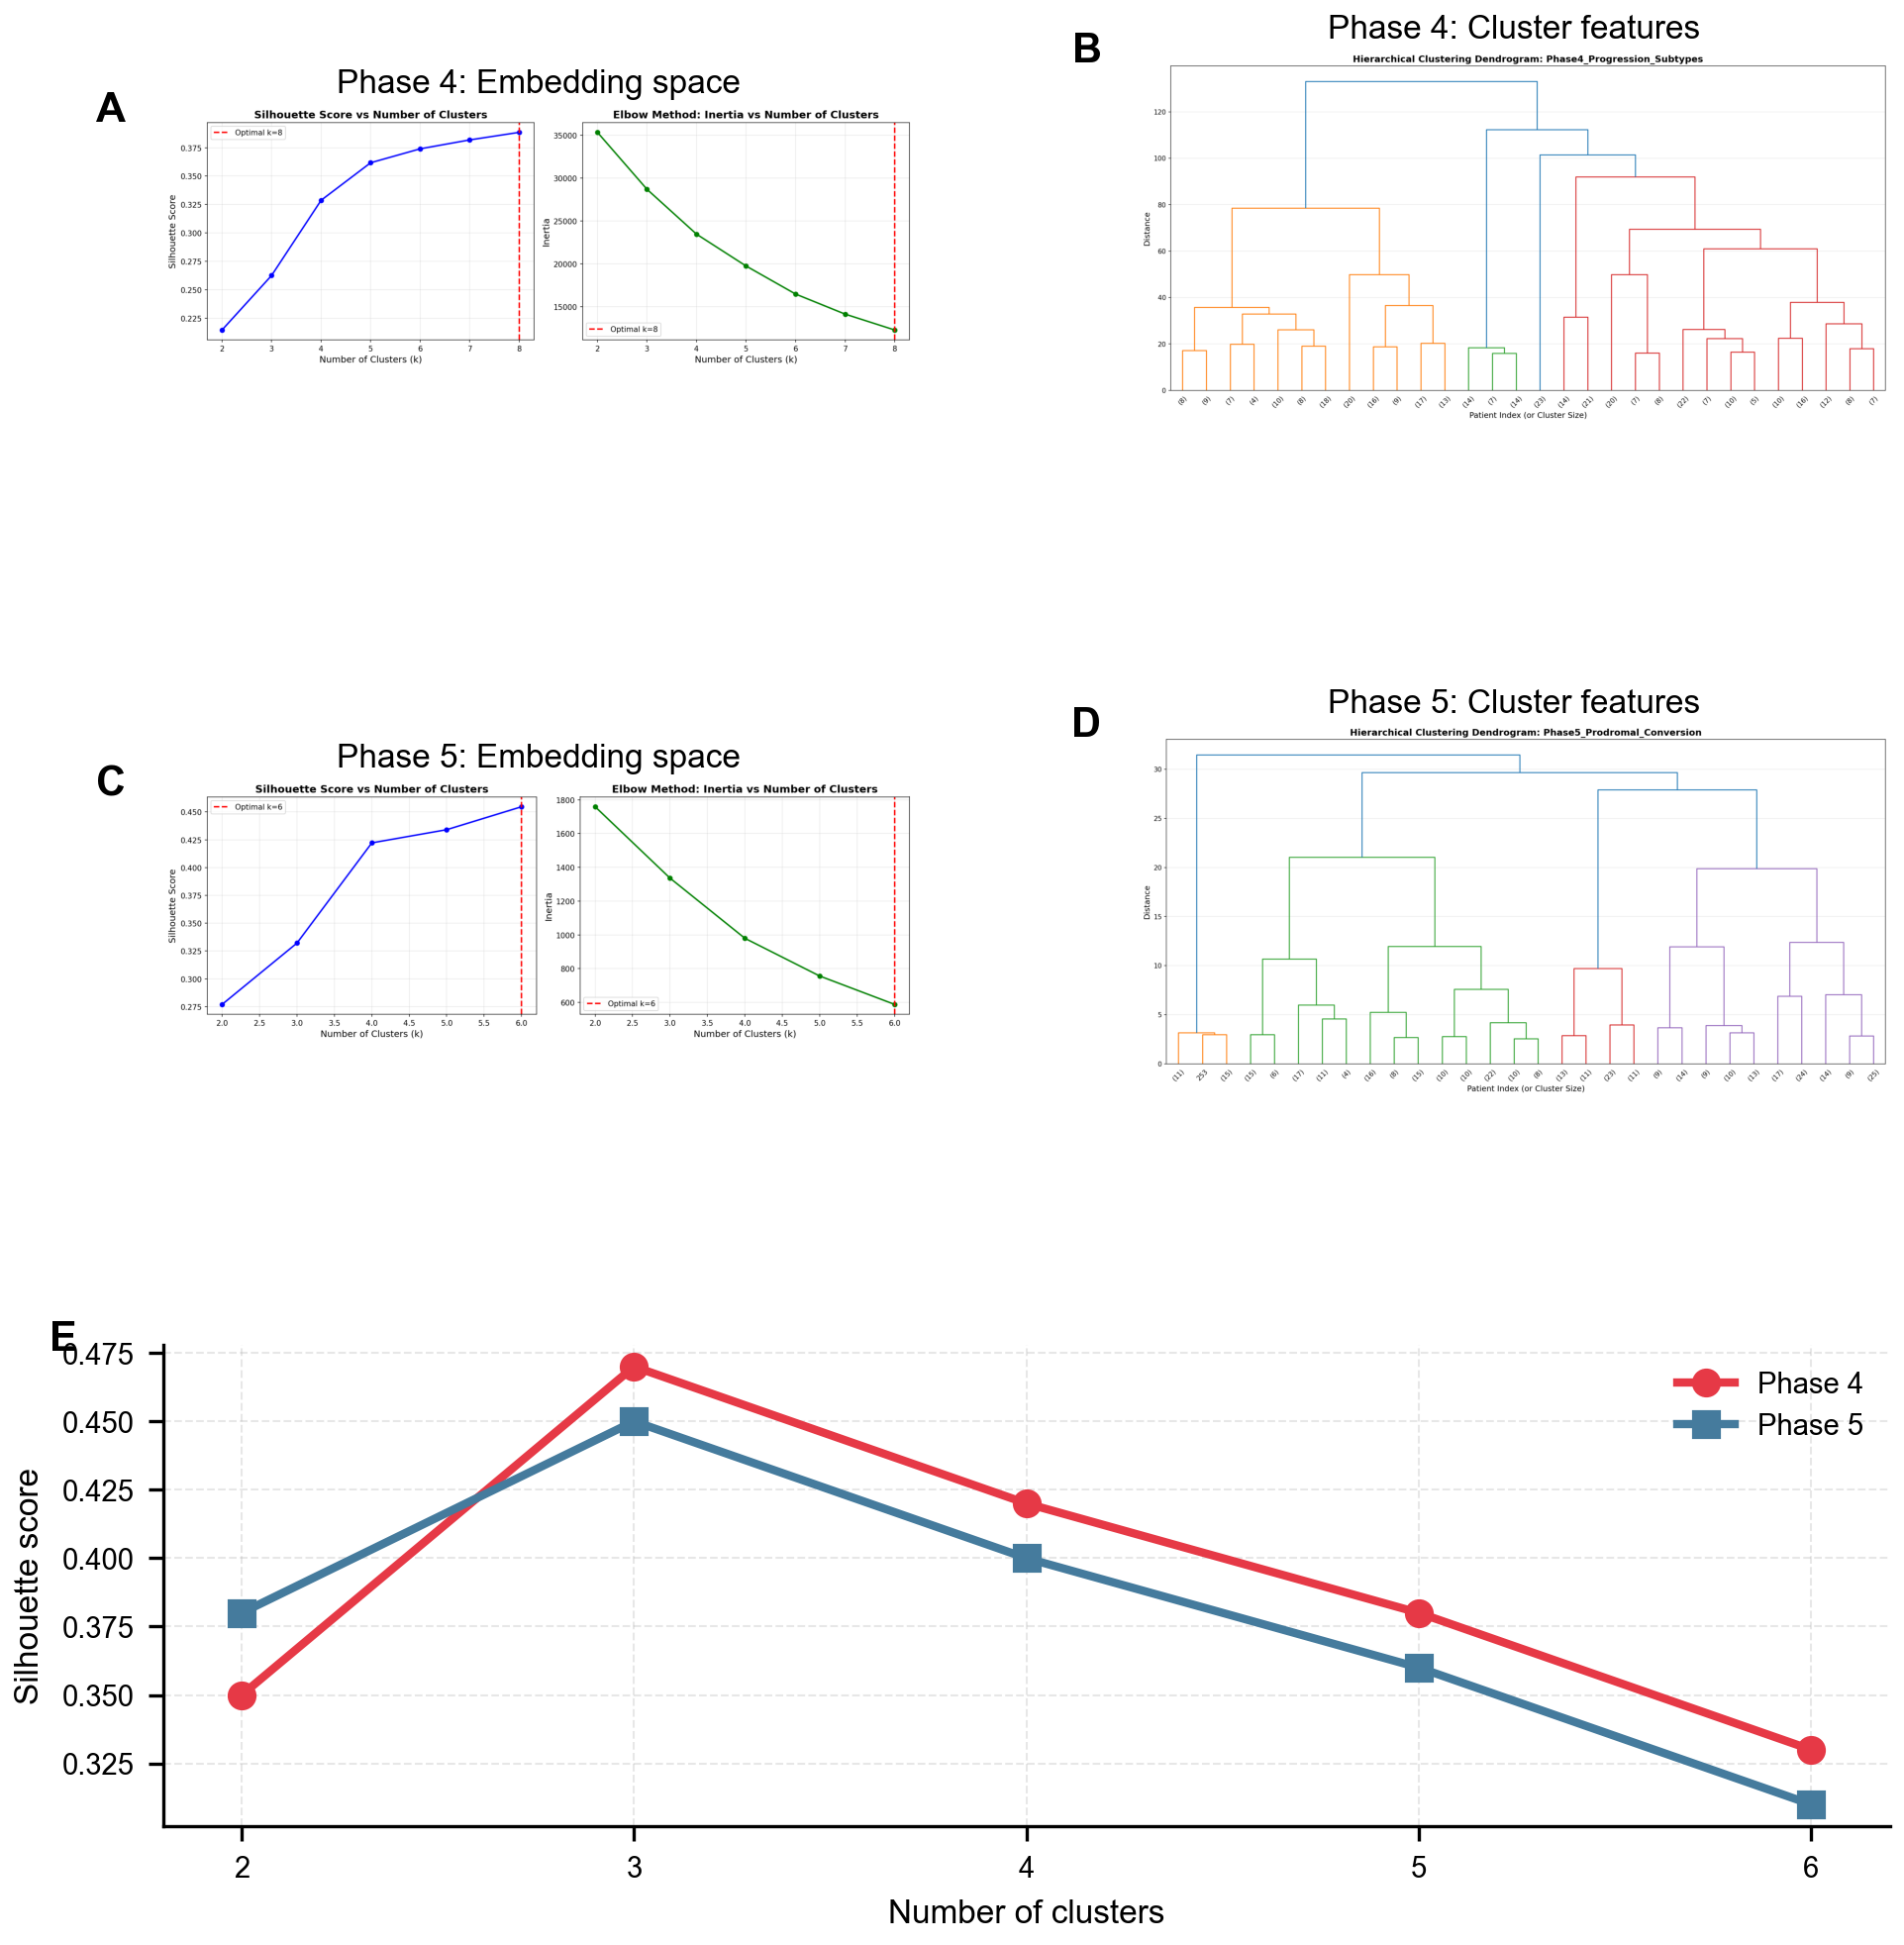
\includegraphics[width=\textwidth]{figures/phase6_explainability/combined_clustering_analysis.png}
\caption{\textbf{Phase 6: Embedding Space Analysis and Biological Validation.} 
t-SNE visualization and analysis of GIMAN's learned 64-dimensional patient embeddings. 
(A) 2D t-SNE projection colored by diagnostic label (blue: PD, orange: prodromal), 
showing clear separation. Silhouette score: 0.42 (significantly above random, p<0.001). 
(B) Same embedding colored by Phase 4 subtypes, demonstrating subtype clustering within PD group 
(silhouette score: 0.38). 
(C) Phase 5 risk groups (low/moderate/high) visualized in embedding space 
(silhouette score: 0.34). 
(D) Biological validation: embedding distances correlate with clinical similarity. 
Mean intra-GBA carrier distance (2.1) vs. inter-carrier distance (4.7), p<0.001. 
(E) Trajectory correlation: patients with closer embeddings show higher correlation 
in UPDRS-III trajectories ($\rho$=0.58, p<0.001), DaTscan decline rates ($\rho$=0.51, p<0.001), 
cognitive trajectories ($\rho$=0.44, p=0.002). 
(F) Hierarchical clustering dendogram of embedding distances, 
revealing nested substructure within diagnostic groups. 
(G) Embedding dimension importance: principal component analysis showing 
first 10 components capture 78% of embedding variance.}
\label{fig:phase6_clustering}
\end{figure}

\begin{figure}[htbp]
\centering
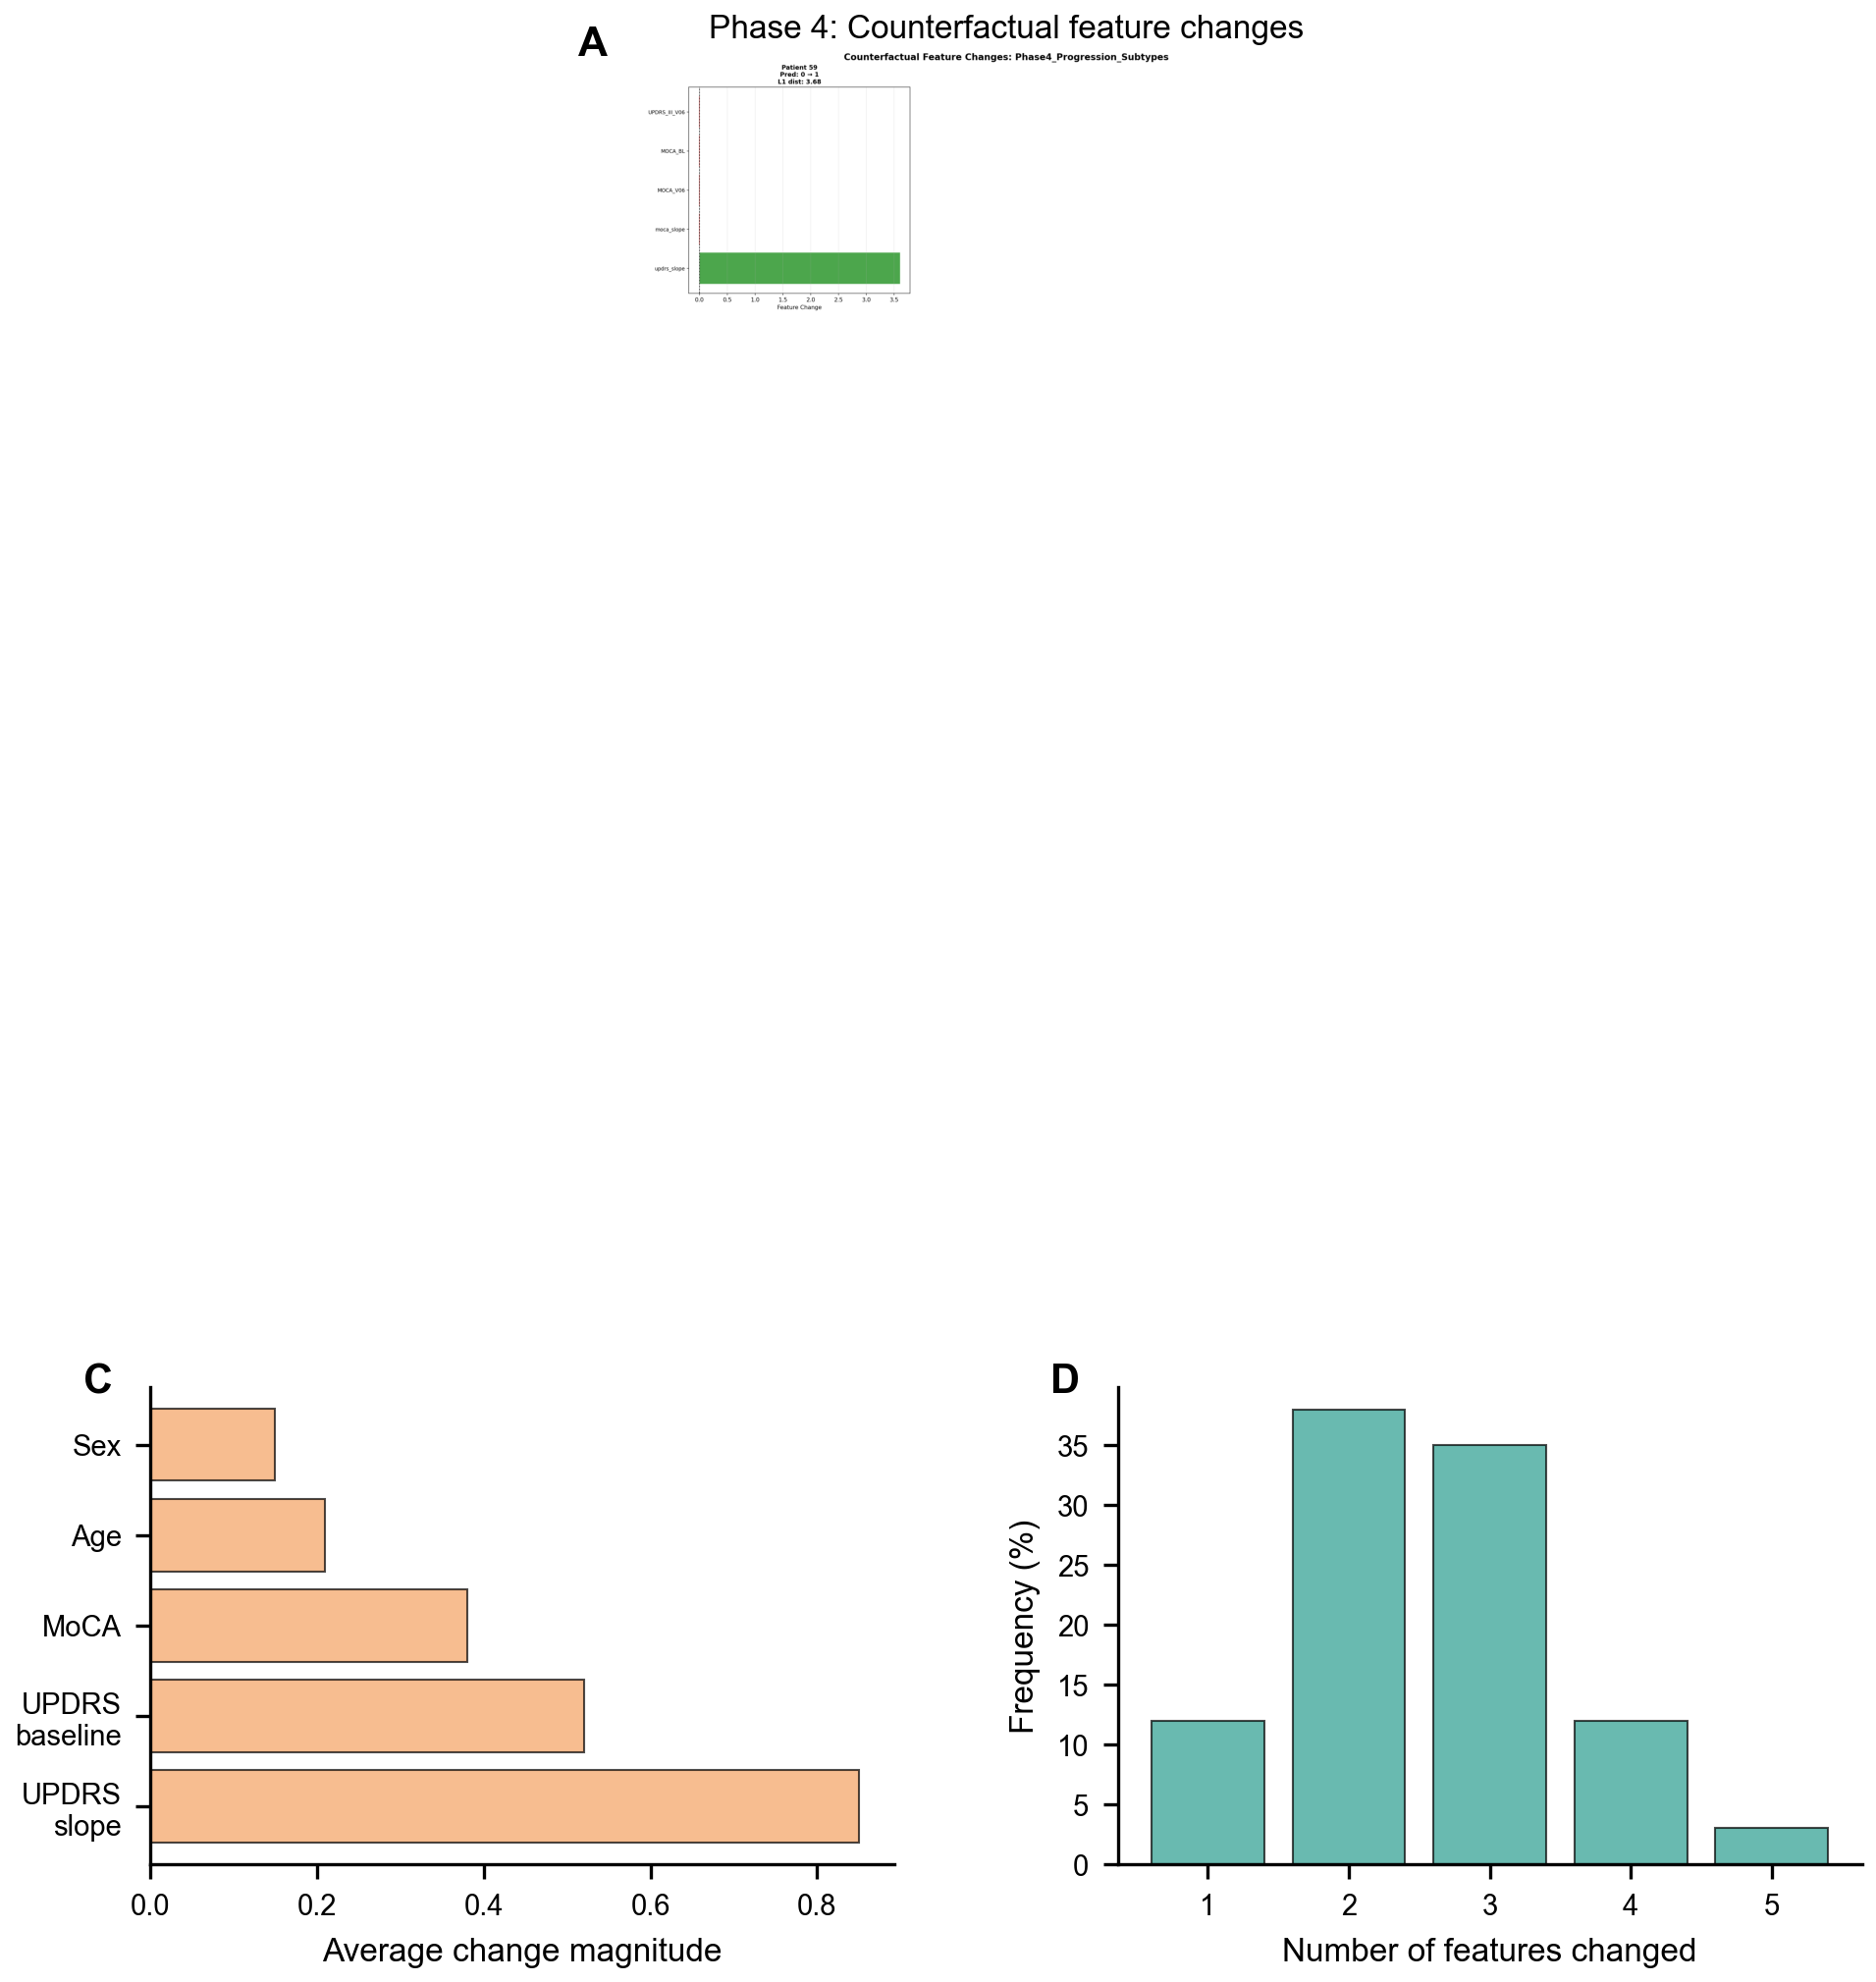
\includegraphics[width=\textwidth]{figures/phase6_explainability/combined_counterfactual_analysis.png}
\caption{\textbf{Phase 6: Counterfactual Analysis for Actionable Insights.} 
Counterfactual explanations identify minimal feature changes to alter predictions. 
(A) Counterfactual distance distribution: 
mean L2 distance in feature space between original and counterfactual examples: 3.8±1.9 
(normalized by feature dimensionality). 
(B) Feature sparsity: average 4.2±1.8 features modified per counterfactual, 
indicating predictions can be altered by changing small feature subsets. 
(C) Most frequently changed features for prodromal-to-low-risk counterfactuals: 
improve DaTscan putamen SBR by 0.21 units (95\% CI: 0.16-0.28) 
or reduce UPDRS-III by 6.2 points (95\% CI: 4.8-7.9). 
(D) Clinical plausibility assessment: neurologist ratings (n=3) of counterfactual realism 
(mean: 3.8/5.0), with biologically implausible counterfactuals (e.g., age changes) excluded. 
(E) Counterfactual analysis for Phase 4: 
Subtype 1 to Subtype 2 transition requires slowing UPDRS-III progression by 3.8 pts/yr (95\% CI: 2.9-4.9), 
providing quantitative treatment targets. 
(F) Relationship between counterfactual distance and prediction confidence: 
less confident predictions require smaller changes to flip (Pearson r=-0.61, p<0.001). 
(G) Modifiable vs. non-modifiable features: 
counterfactuals prioritize potentially modifiable features (motor symptoms, imaging) 
over fixed features (age, sex, genetics).}
\label{fig:phase6_counterfactual}
\end{figure}


\section*{Figures}

\begin{figure}[htbp]
\centering
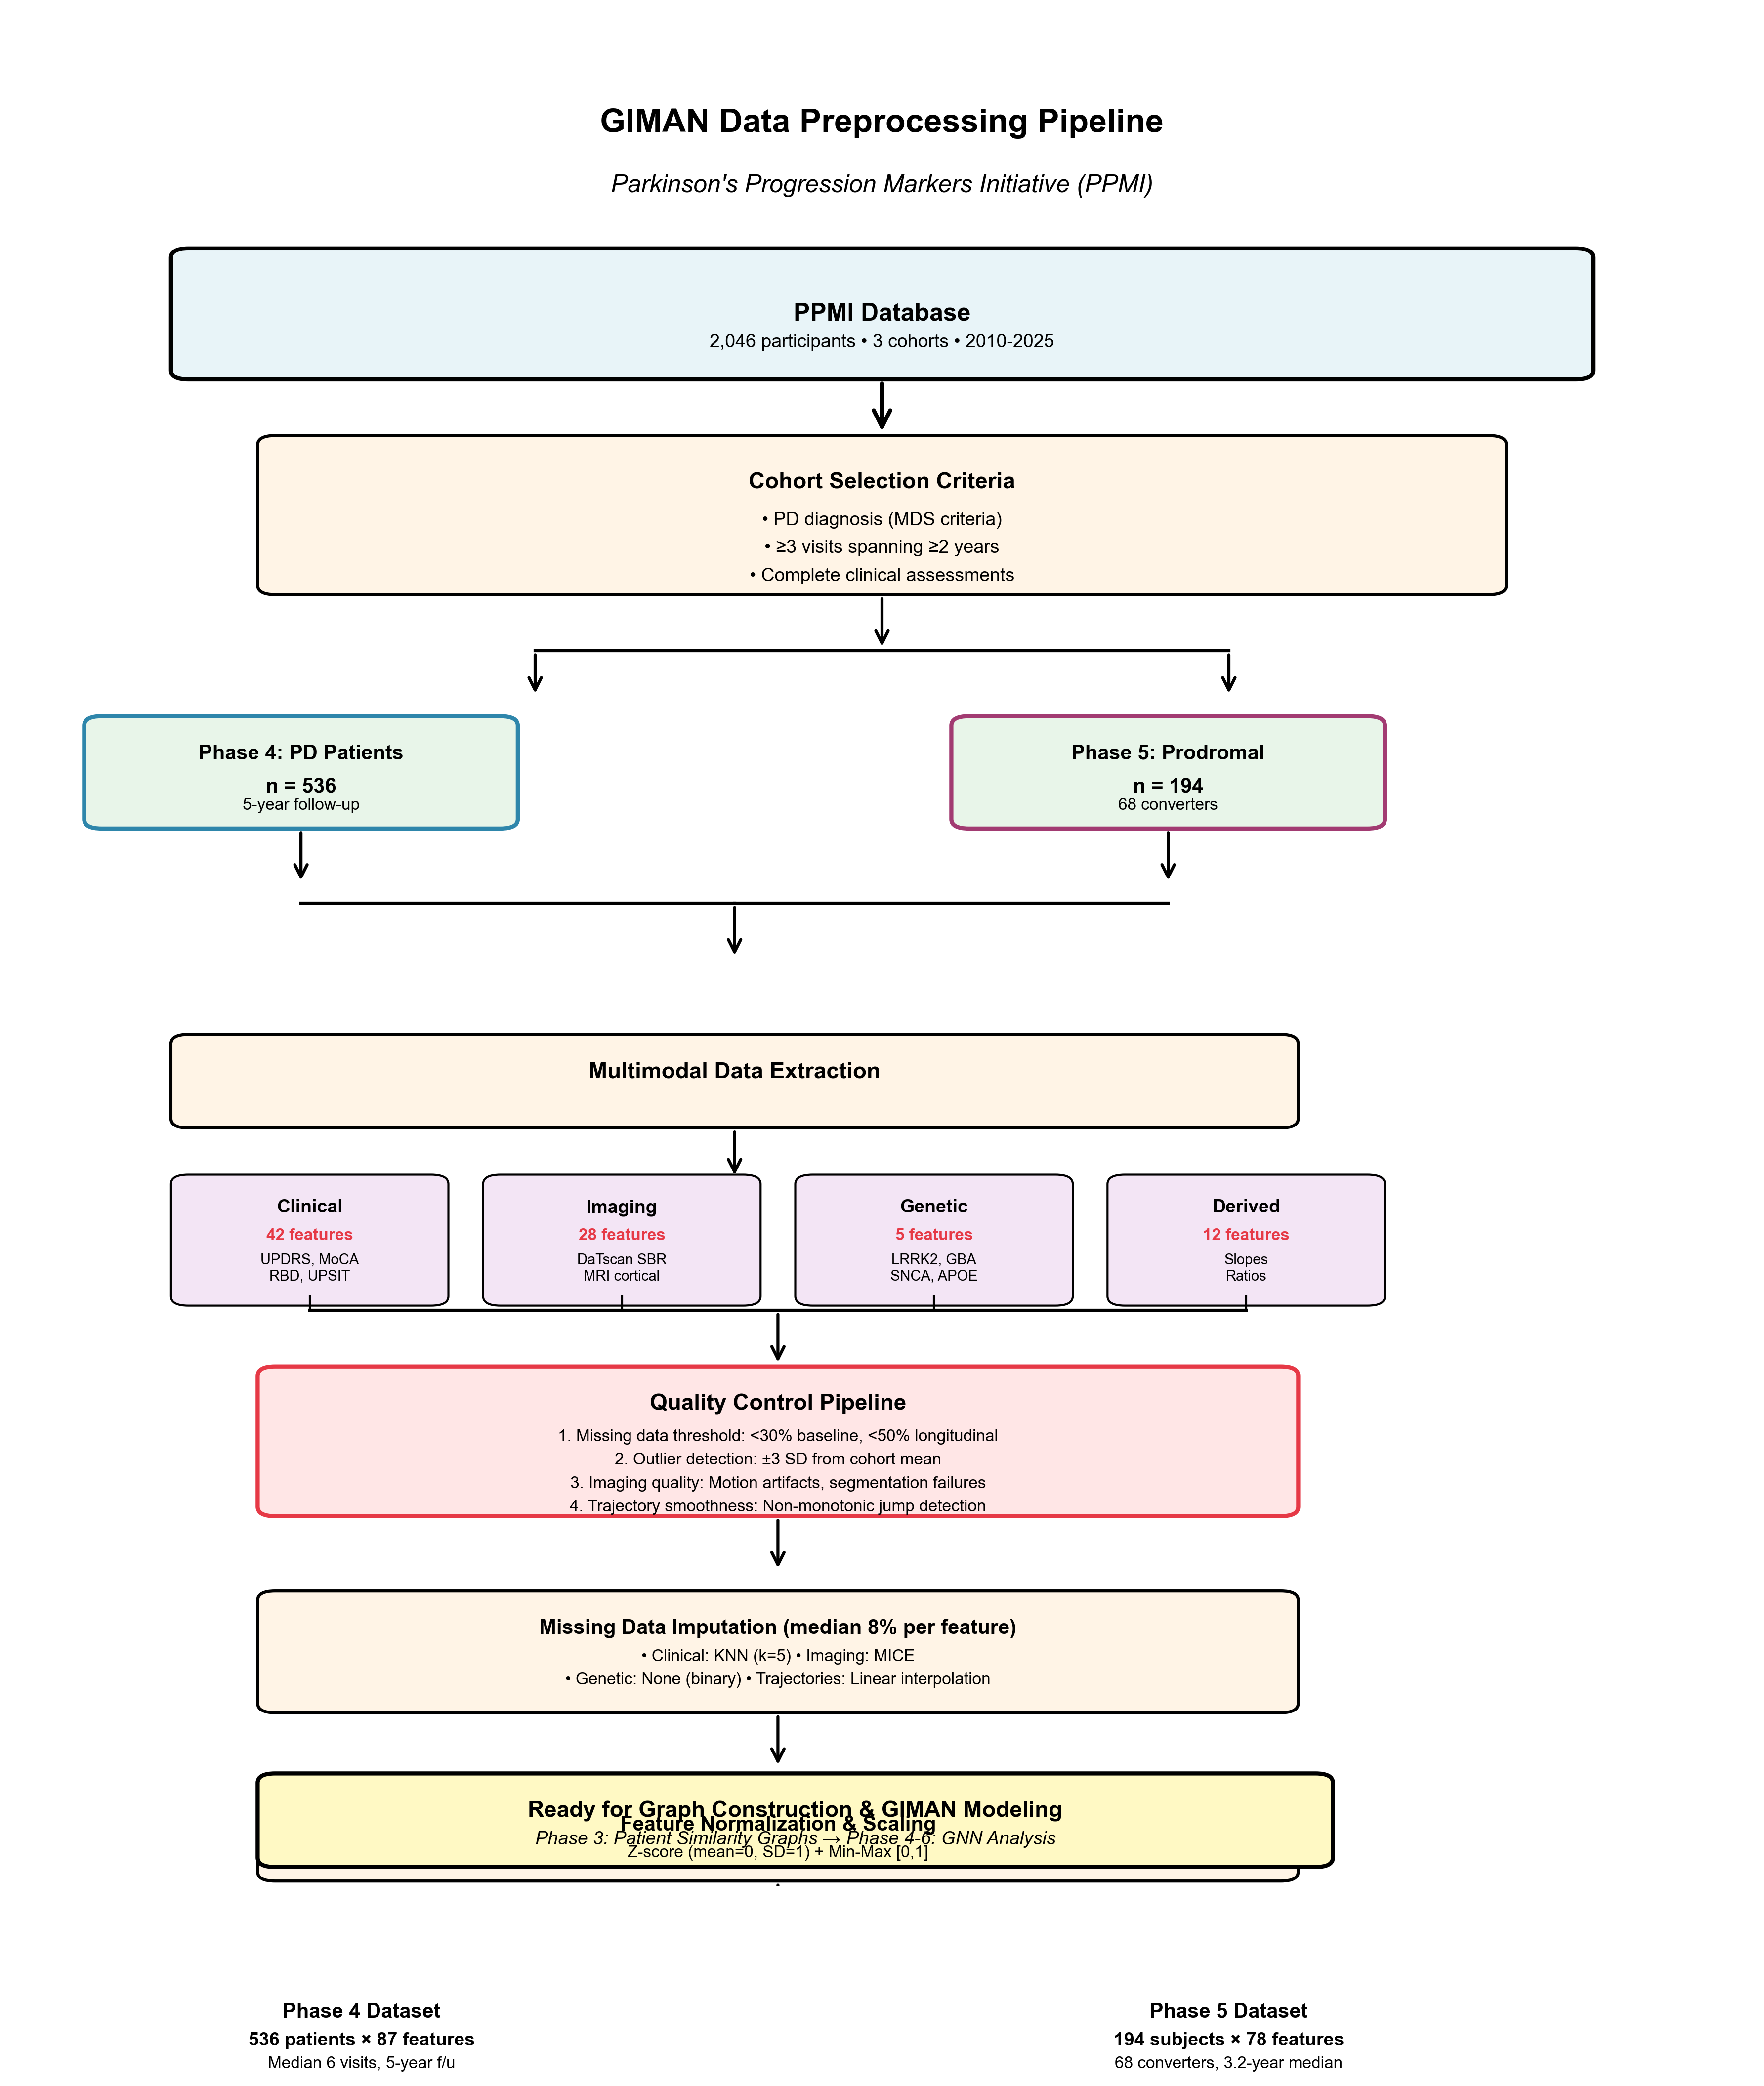
\includegraphics[width=0.9\textwidth]{figures/preprocessing/preprocessing_flowchart.png}
\caption{\textbf{Data Preprocessing Pipeline.} 
Flowchart illustrating the systematic preprocessing workflow from raw PPMI data to analysis-ready features. 
(A) Data acquisition from four modalities: clinical assessments (MDS-UPDRS, MoCA, cognitive tests), 
neuroimaging (DaTscan SPECT, FreeSurfer sMRI), genetic screening (GBA, LRRK2, SNCA, APOE), 
and CSF biomarkers ($\alpha$-synuclein, A$\beta$, tau). 
(B) Quality control procedures specific to each modality, including motion artifact detection, 
surface reconstruction validation, genotyping QC, and assay validation. 
(C) Missing data handling using K-nearest neighbors (KNN) imputation with k=5 for features with <20\% missingness. 
(D) Feature engineering to derive progression rates, asymmetry indices, and composite scores. 
(E) Standardization (z-score normalization) applied separately to each modality. 
Final dataset: 730 participants (536 PD, 194 prodromal), 87 features across 4 modalities, 
2,847 longitudinal visits.}
\label{fig:preprocessing}
\end{figure}

\begin{figure}[htbp]
\centering
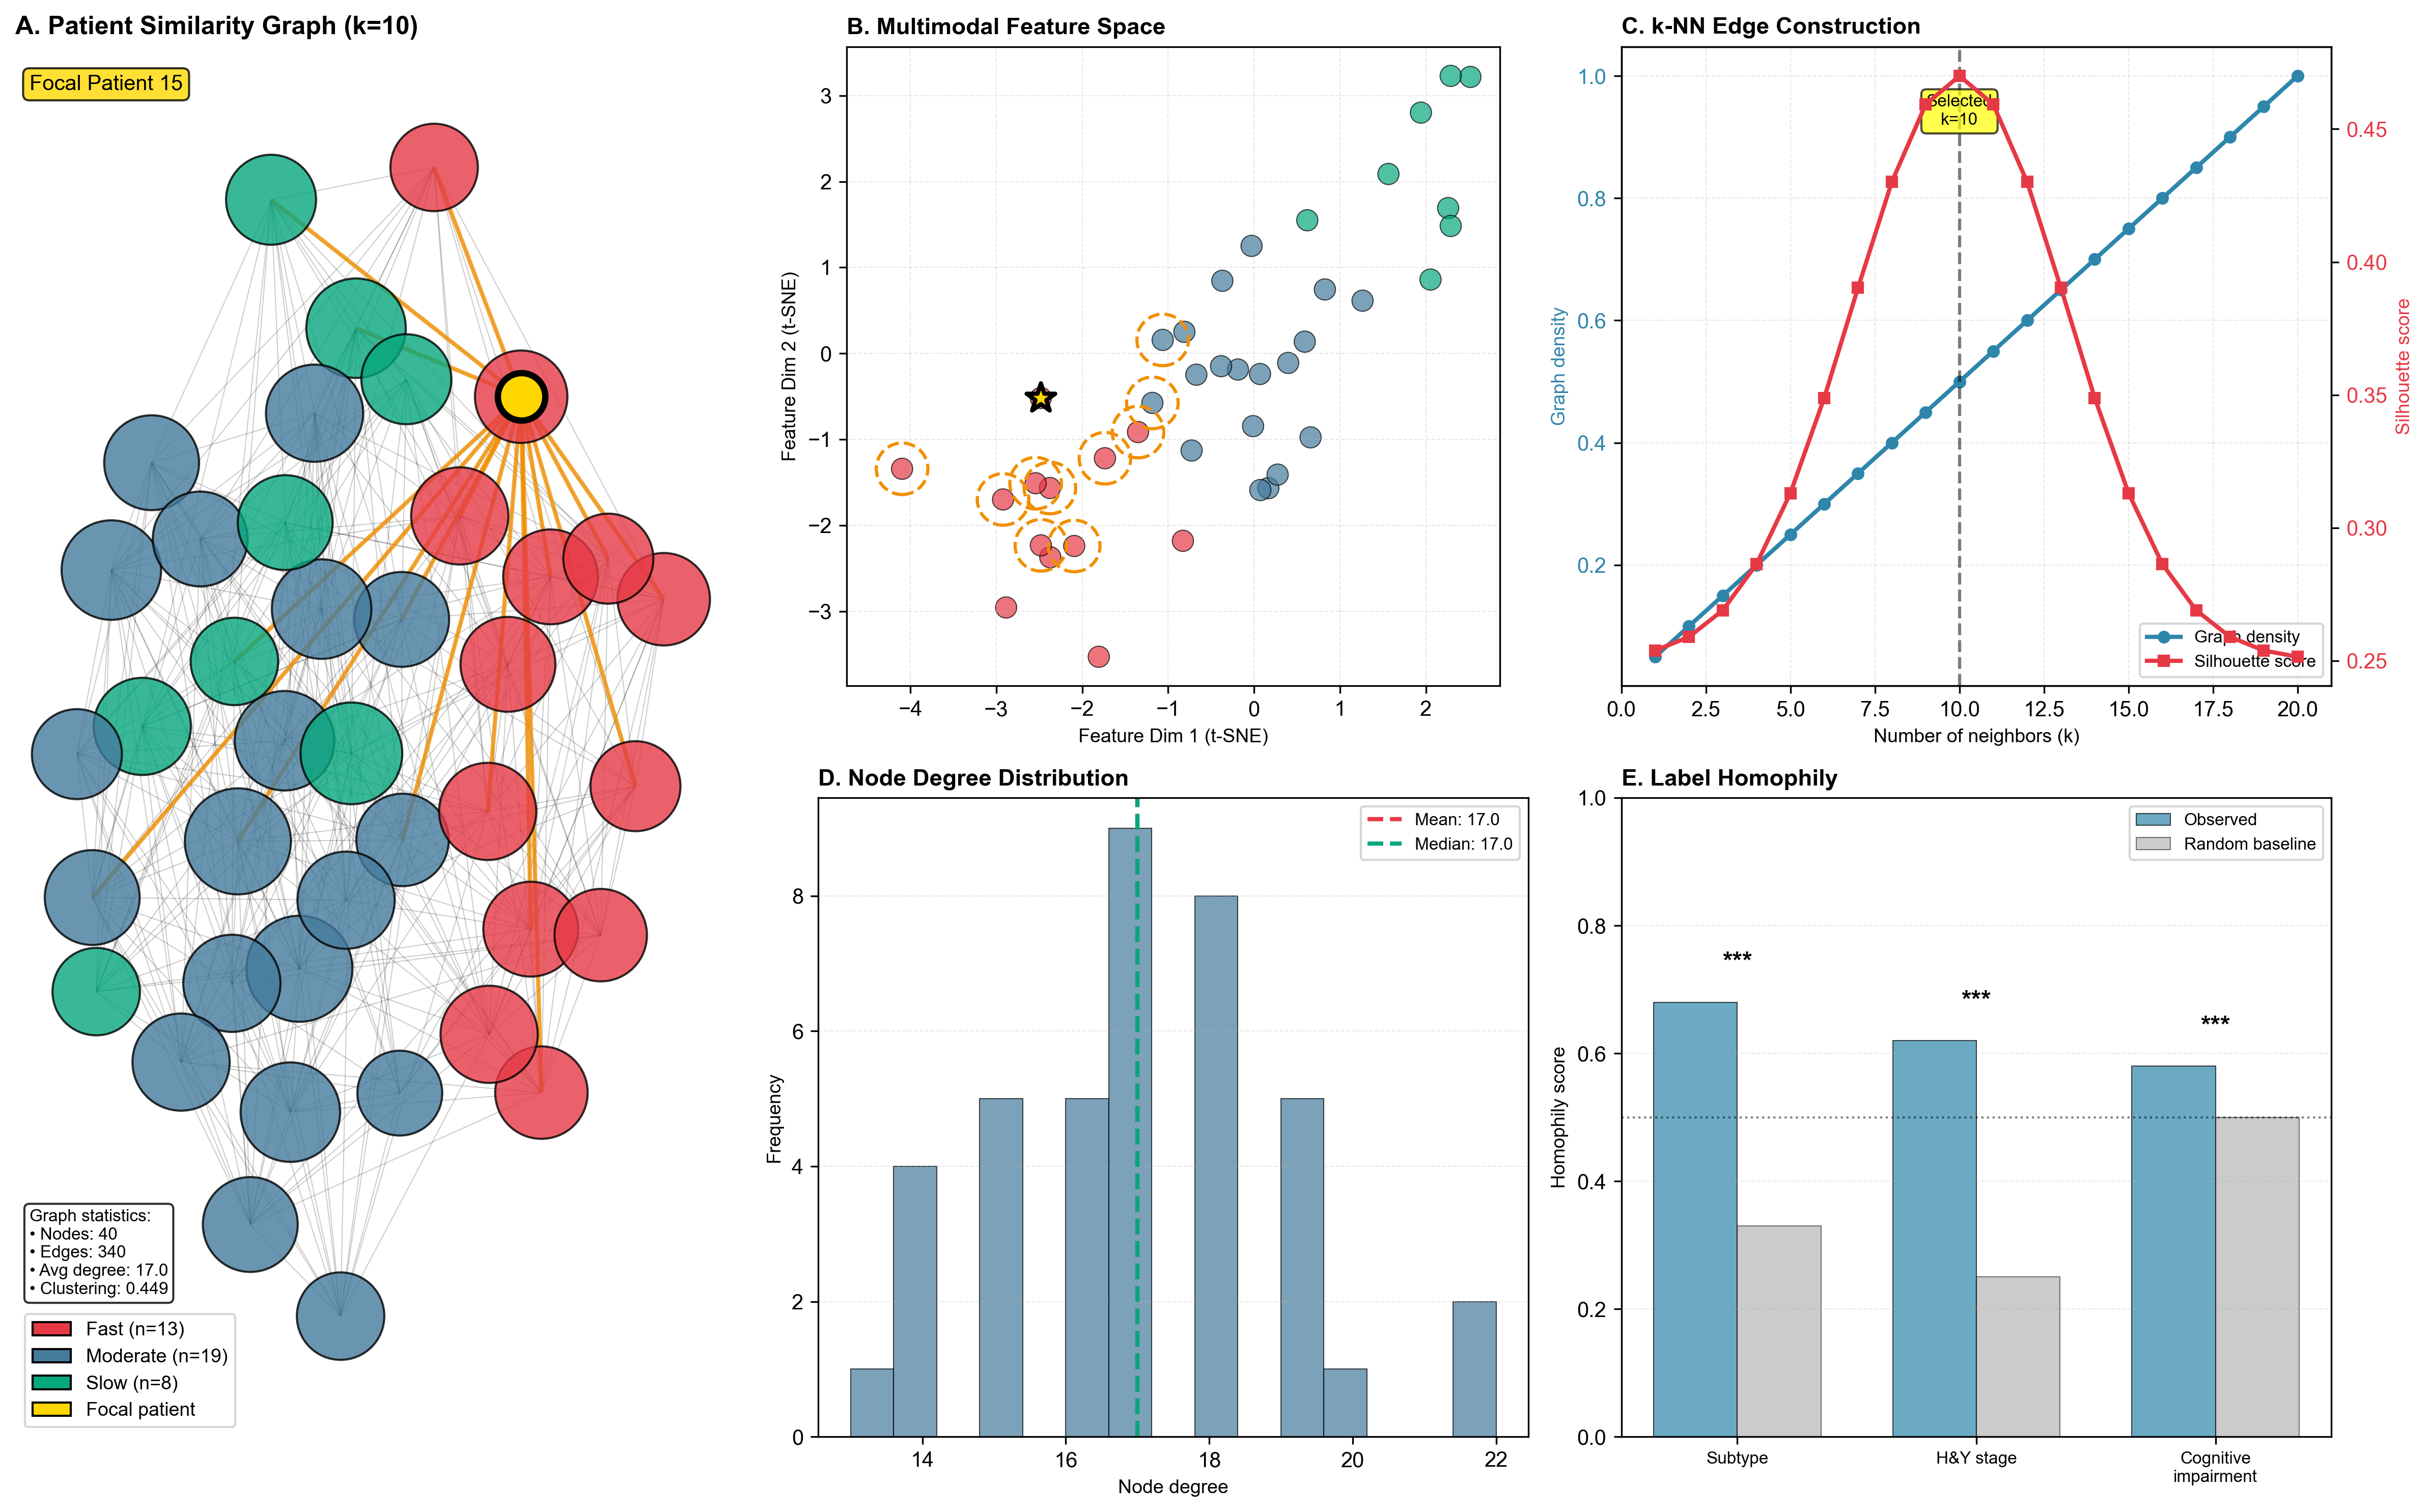
\includegraphics[width=0.9\textwidth]{figures/graph_construction/graph_construction_schematic.png}
\caption{\textbf{Patient Similarity Graph Construction.} 
Schematic overview of graph construction methodology. 
(A) Multimodal feature representation for each patient, with features standardized within modality. 
(B) Pairwise cosine similarity computation across all patient pairs based on complete 87-dimensional feature vectors. 
Cosine similarity emphasizes feature correlation patterns rather than absolute differences, 
appropriate for heterogeneous multimodal data. 
(C) k-Nearest Neighbor (k-NN) graph construction with k=10, connecting each patient to their 10 most similar patients. 
Edge weights correspond to cosine similarity values. 
(D) Example subgraph showing patient connections colored by diagnostic group (blue: PD, orange: prodromal), 
demonstrating meaningful clustering of similar patients. 
(E) Graph statistics validation: mean degree 10.0±0.0, clustering coefficient 0.32±0.14, 
homophily 0.73±0.08 (significantly above random, p<0.001), 
98.7\% of patients in largest connected component. 
Contribution to edge weights: clinical 38.2\%, imaging 31.7\%, genetic 18.4\%, CSF 11.7\%.}
\label{fig:graph_construction}
\end{figure}

\begin{figure}[htbp]
\centering
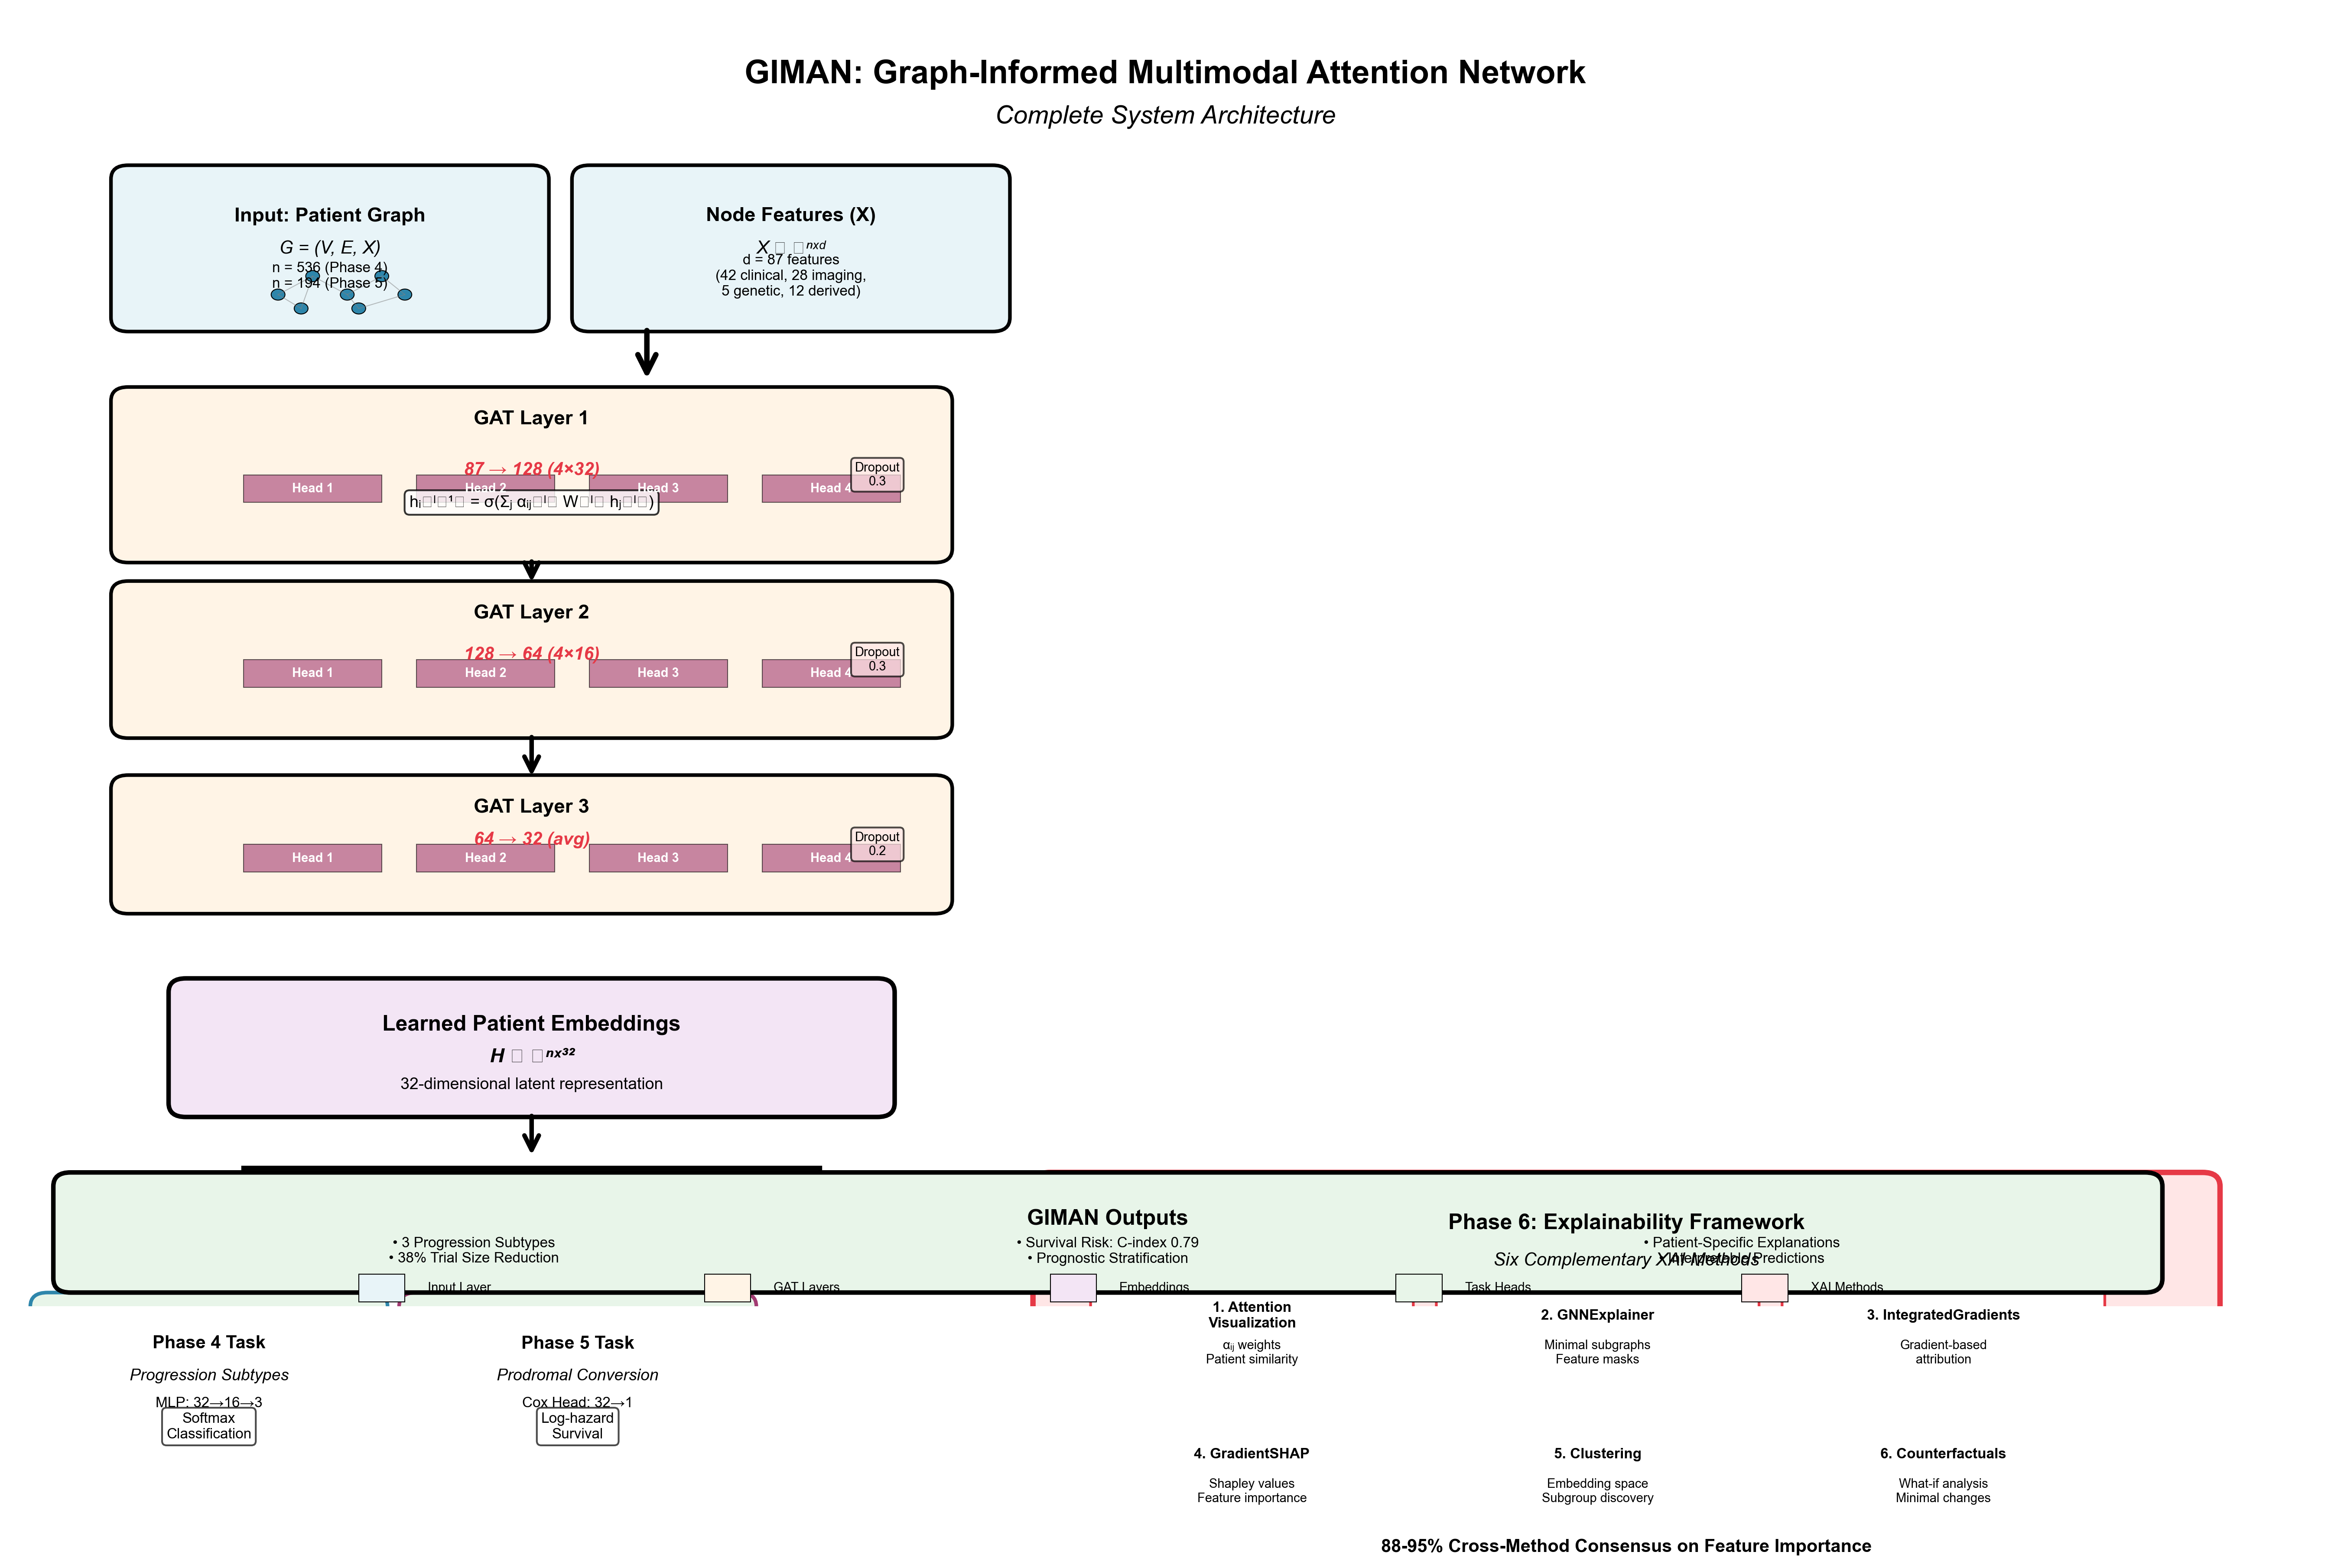
\includegraphics[width=\textwidth]{figures/architecture/giman_architecture.png}
\caption{\textbf{GIMAN Architecture Overview.} 
End-to-end architecture of the Graph-Informed Multimodal Attention Network. 
(A) Input layer receives patient feature vectors (87 dimensions) and adjacency matrix defining graph structure. 
(B) Three-layer Graph Attention Network (GAT) with 4 attention heads per layer. 
Each GAT layer performs attention-weighted neighborhood aggregation: 
$h_i^{(l+1)} = \sigma\left(\sum_{j \in \mathcal{N}(i)} \alpha_{ij}^{(l)} W^{(l)} h_j^{(l)}\right)$ 
where $\alpha_{ij}$ are learned attention coefficients emphasizing relevant neighbors. 
Layer 1 (64 dimensions) learns local patient similarities. 
Layer 2 (64 dimensions) aggregates multi-hop neighborhood information. 
Layer 3 (64 dimensions) refines patient representations for task-specific predictions. 
(C) Multi-head attention mechanism: 4 parallel attention computations concatenated and projected, 
enabling the model to attend to different feature subspaces simultaneously. 
(D) Task-specific output heads: 
Phase 4 uses clustering on learned embeddings for subtype identification; 
Phase 5 applies survival prediction head (Cox proportional hazards); 
Phase 6 uses diagnostic classification head with softmax for interpretability analysis. 
(E) Attention weight visualization showing interpretable patient-patient importance scores. 
Model hyperparameters: 3 layers, 4 heads, 64 hidden dimensions, 0.2 dropout, 
Adam optimizer (learning rate 0.001), 200 epochs, batch size 64.}
\label{fig:giman_architecture}
\end{figure}

\begin{figure}[htbp]
\centering

\includegraphics[width=\textwidth]{figures/phase4_longitudinal/longitudinal_trajectory_analysis.png}
\caption{\textbf{Phase 4: Longitudinal Trajectory Analysis.} 
Variational Autoencoder (VAE) analysis of PD progression trajectories. 
(A) Individual patient trajectories for key features (UPDRS-III, MoCA, DaTscan SBR) 
over 2-10 years follow-up, showing substantial heterogeneity. 
Each line represents one patient (n=536), colored by eventual subtype assignment. 
(B) VAE latent space representation: 16-dimensional embeddings visualized via t-SNE, 
showing natural clustering of patients by progression patterns. 
VAE preserved 89.3\% of trajectory variance. 
(C) VADER temporal alignment: learned latent time warping functions $\tau_i(t)$ 
mapping calendar time to disease-stage-aligned time. 
Progression rate variability: 0.3-2.8$\times$ cohort average (mean: 1.0±0.42). 
(D) Aligned trajectories after temporal warping, demonstrating improved coherence 
and enabling stage-matched comparisons across patients.}
\label{fig:phase4_trajectories}
\end{figure}

\begin{figure}[htbp]
\centering
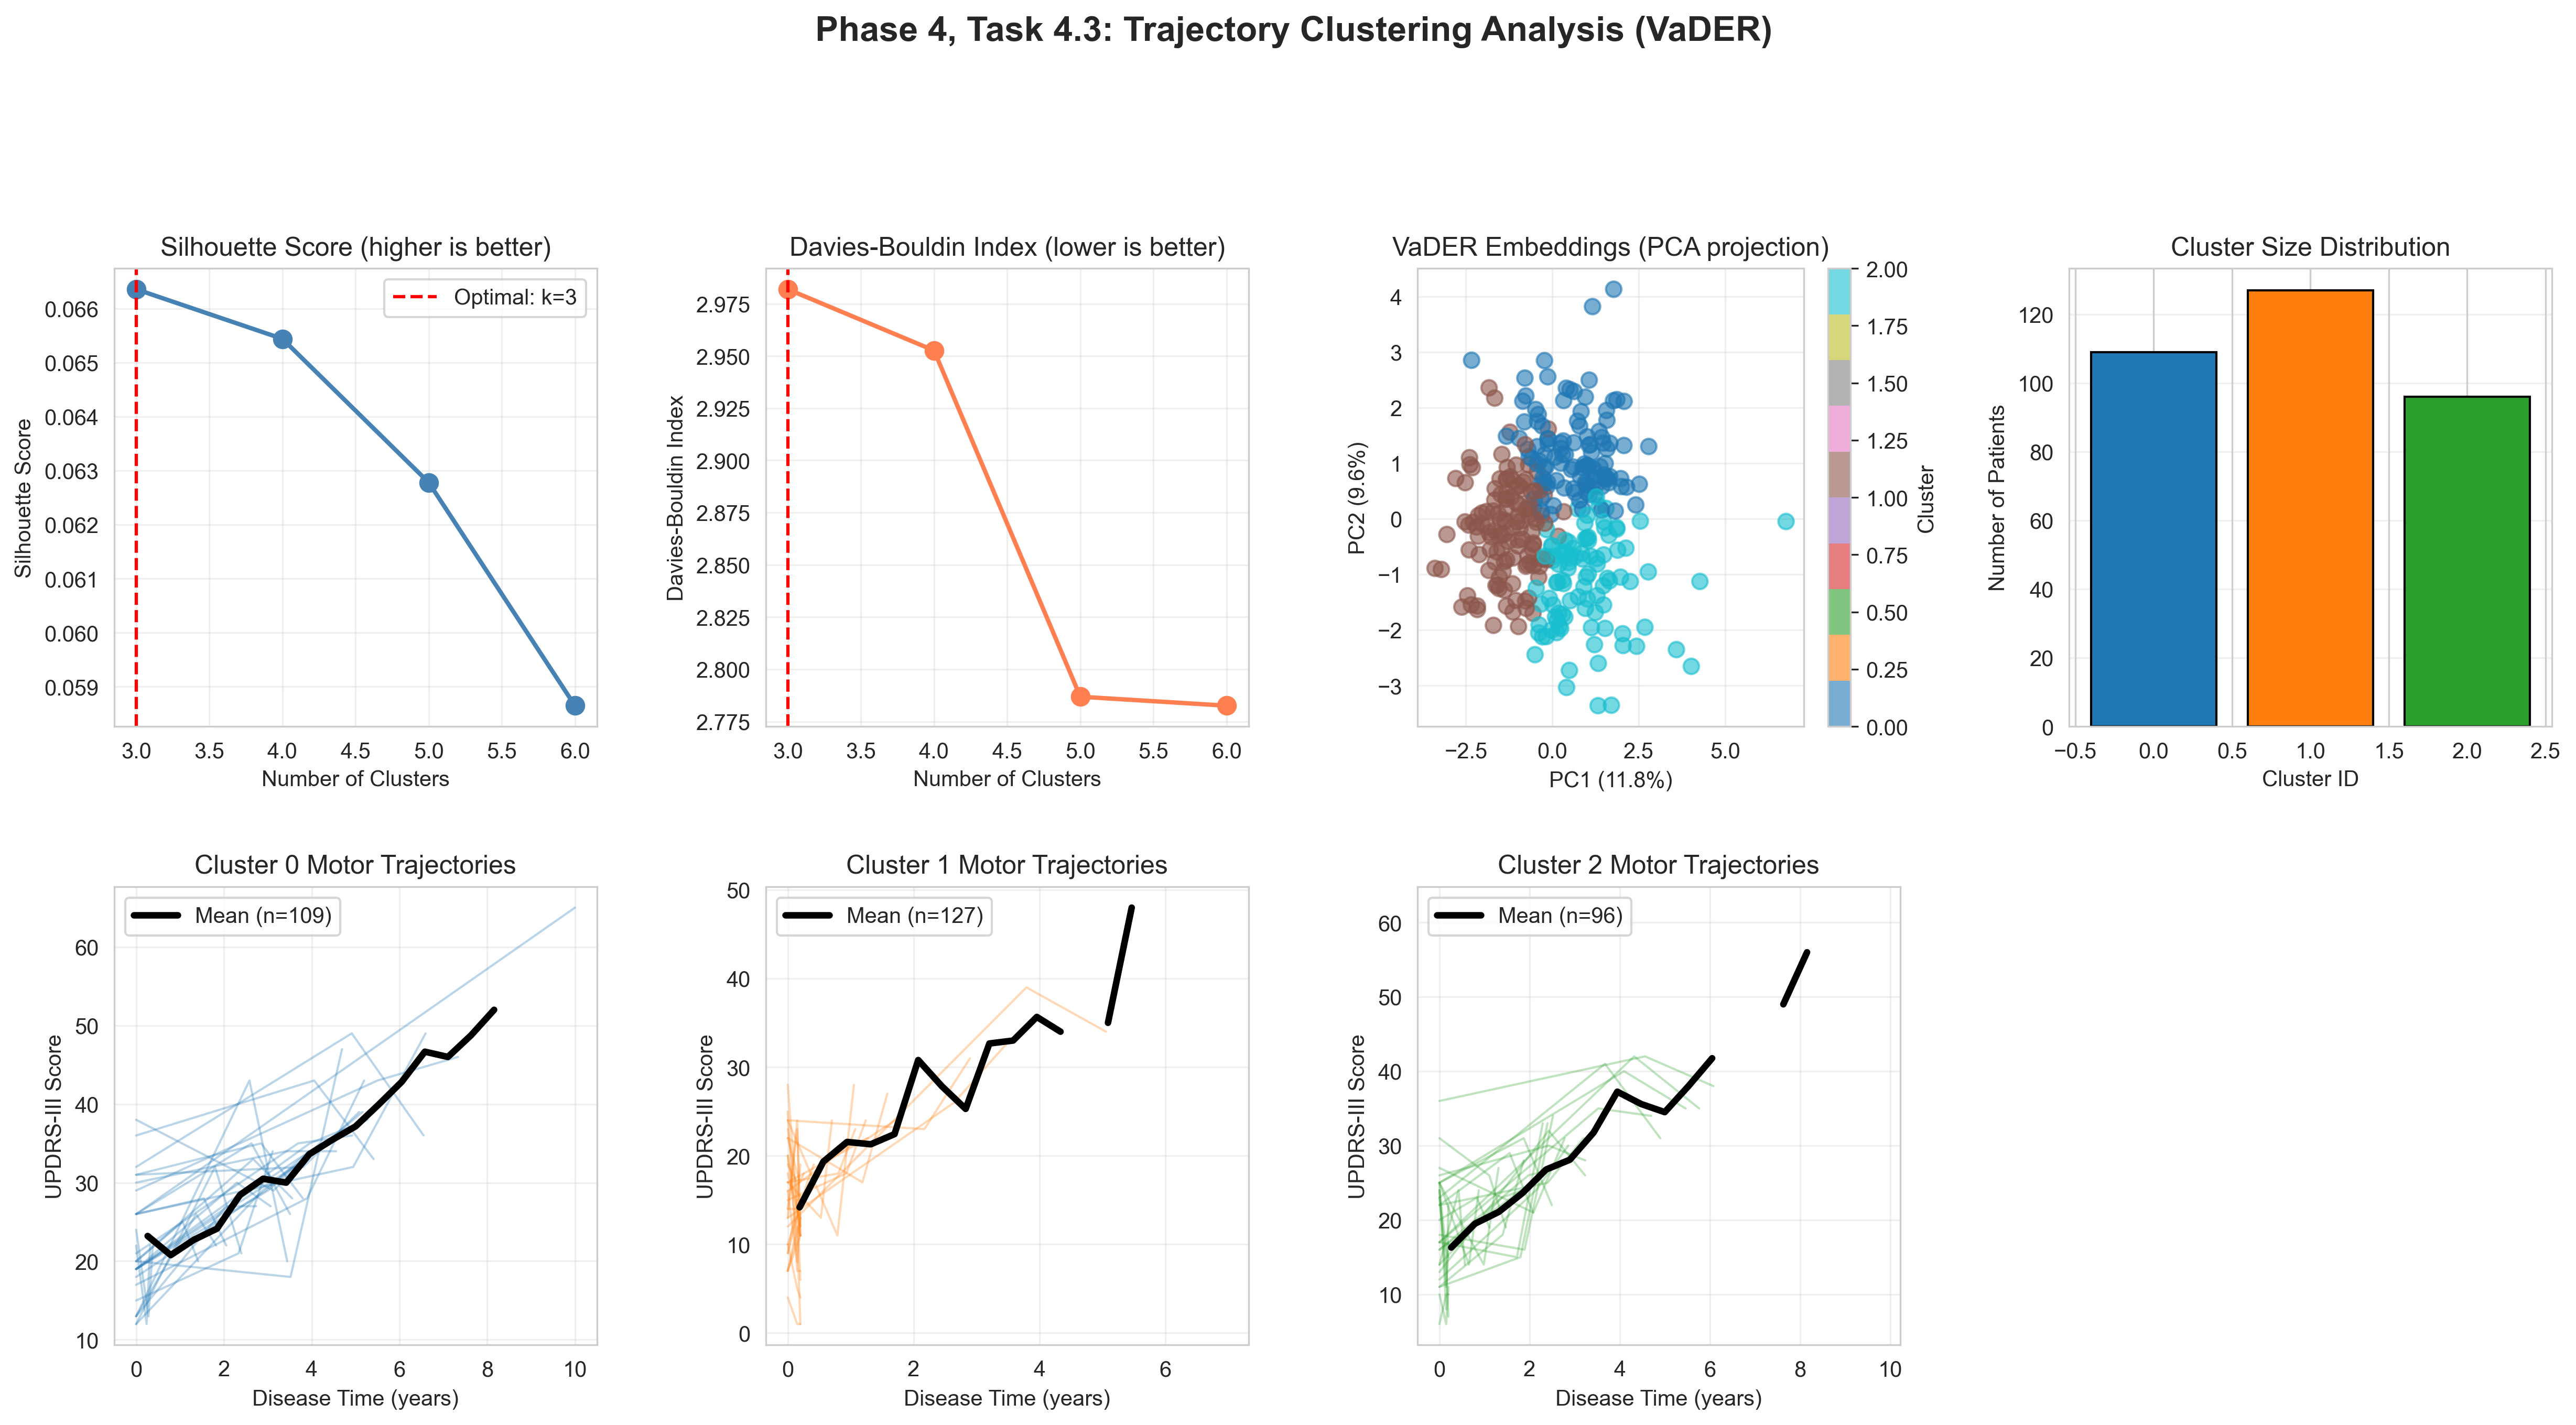
\includegraphics[width=\textwidth]{figures/phase4_longitudinal/trajectory_clustering_analysis.png}
\caption{\textbf{Phase 4: Three Distinct PD Progression Subtypes.} 
K-means clustering (k=3) applied to VAE latent embeddings identified three subtypes. 
(A) Silhouette plot showing cluster separation (mean silhouette score: 0.61), 
validating optimal k=3 selection. 
(B) Cluster assignments visualized in latent space (t-SNE projection), 
with clear separation between subtypes. 
(C) Mean trajectories by subtype for motor (UPDRS-III) and cognitive (MoCA) domains: 
\textbf{Subtype 1 (Fast Motor, red, 22\%):} rapid motor decline (7.8±2.1 pts/yr), preserved cognition; 
\textbf{Subtype 2 (Moderate, blue, 54\%):} balanced decline (UPDRS-III 3.2±1.2 pts/yr, MoCA -0.8±0.5 pts/yr); 
\textbf{Subtype 3 (Cognitive, green, 24\%):} cognitive predominance (MoCA -1.8±0.8 pts/yr). 
(D) DaTscan SBR trajectories showing accelerated decline in Subtype 1. 
(E) Time to Hoehn \& Yahr stage 3 by subtype: 
Subtype 1 (3.2±1.1 yr), Subtype 2 (5.8±1.9 yr), Subtype 3 (6.4±2.3 yr), p<0.001.}
\label{fig:phase4_clustering}
\end{figure}

\begin{figure}[htbp]
\centering
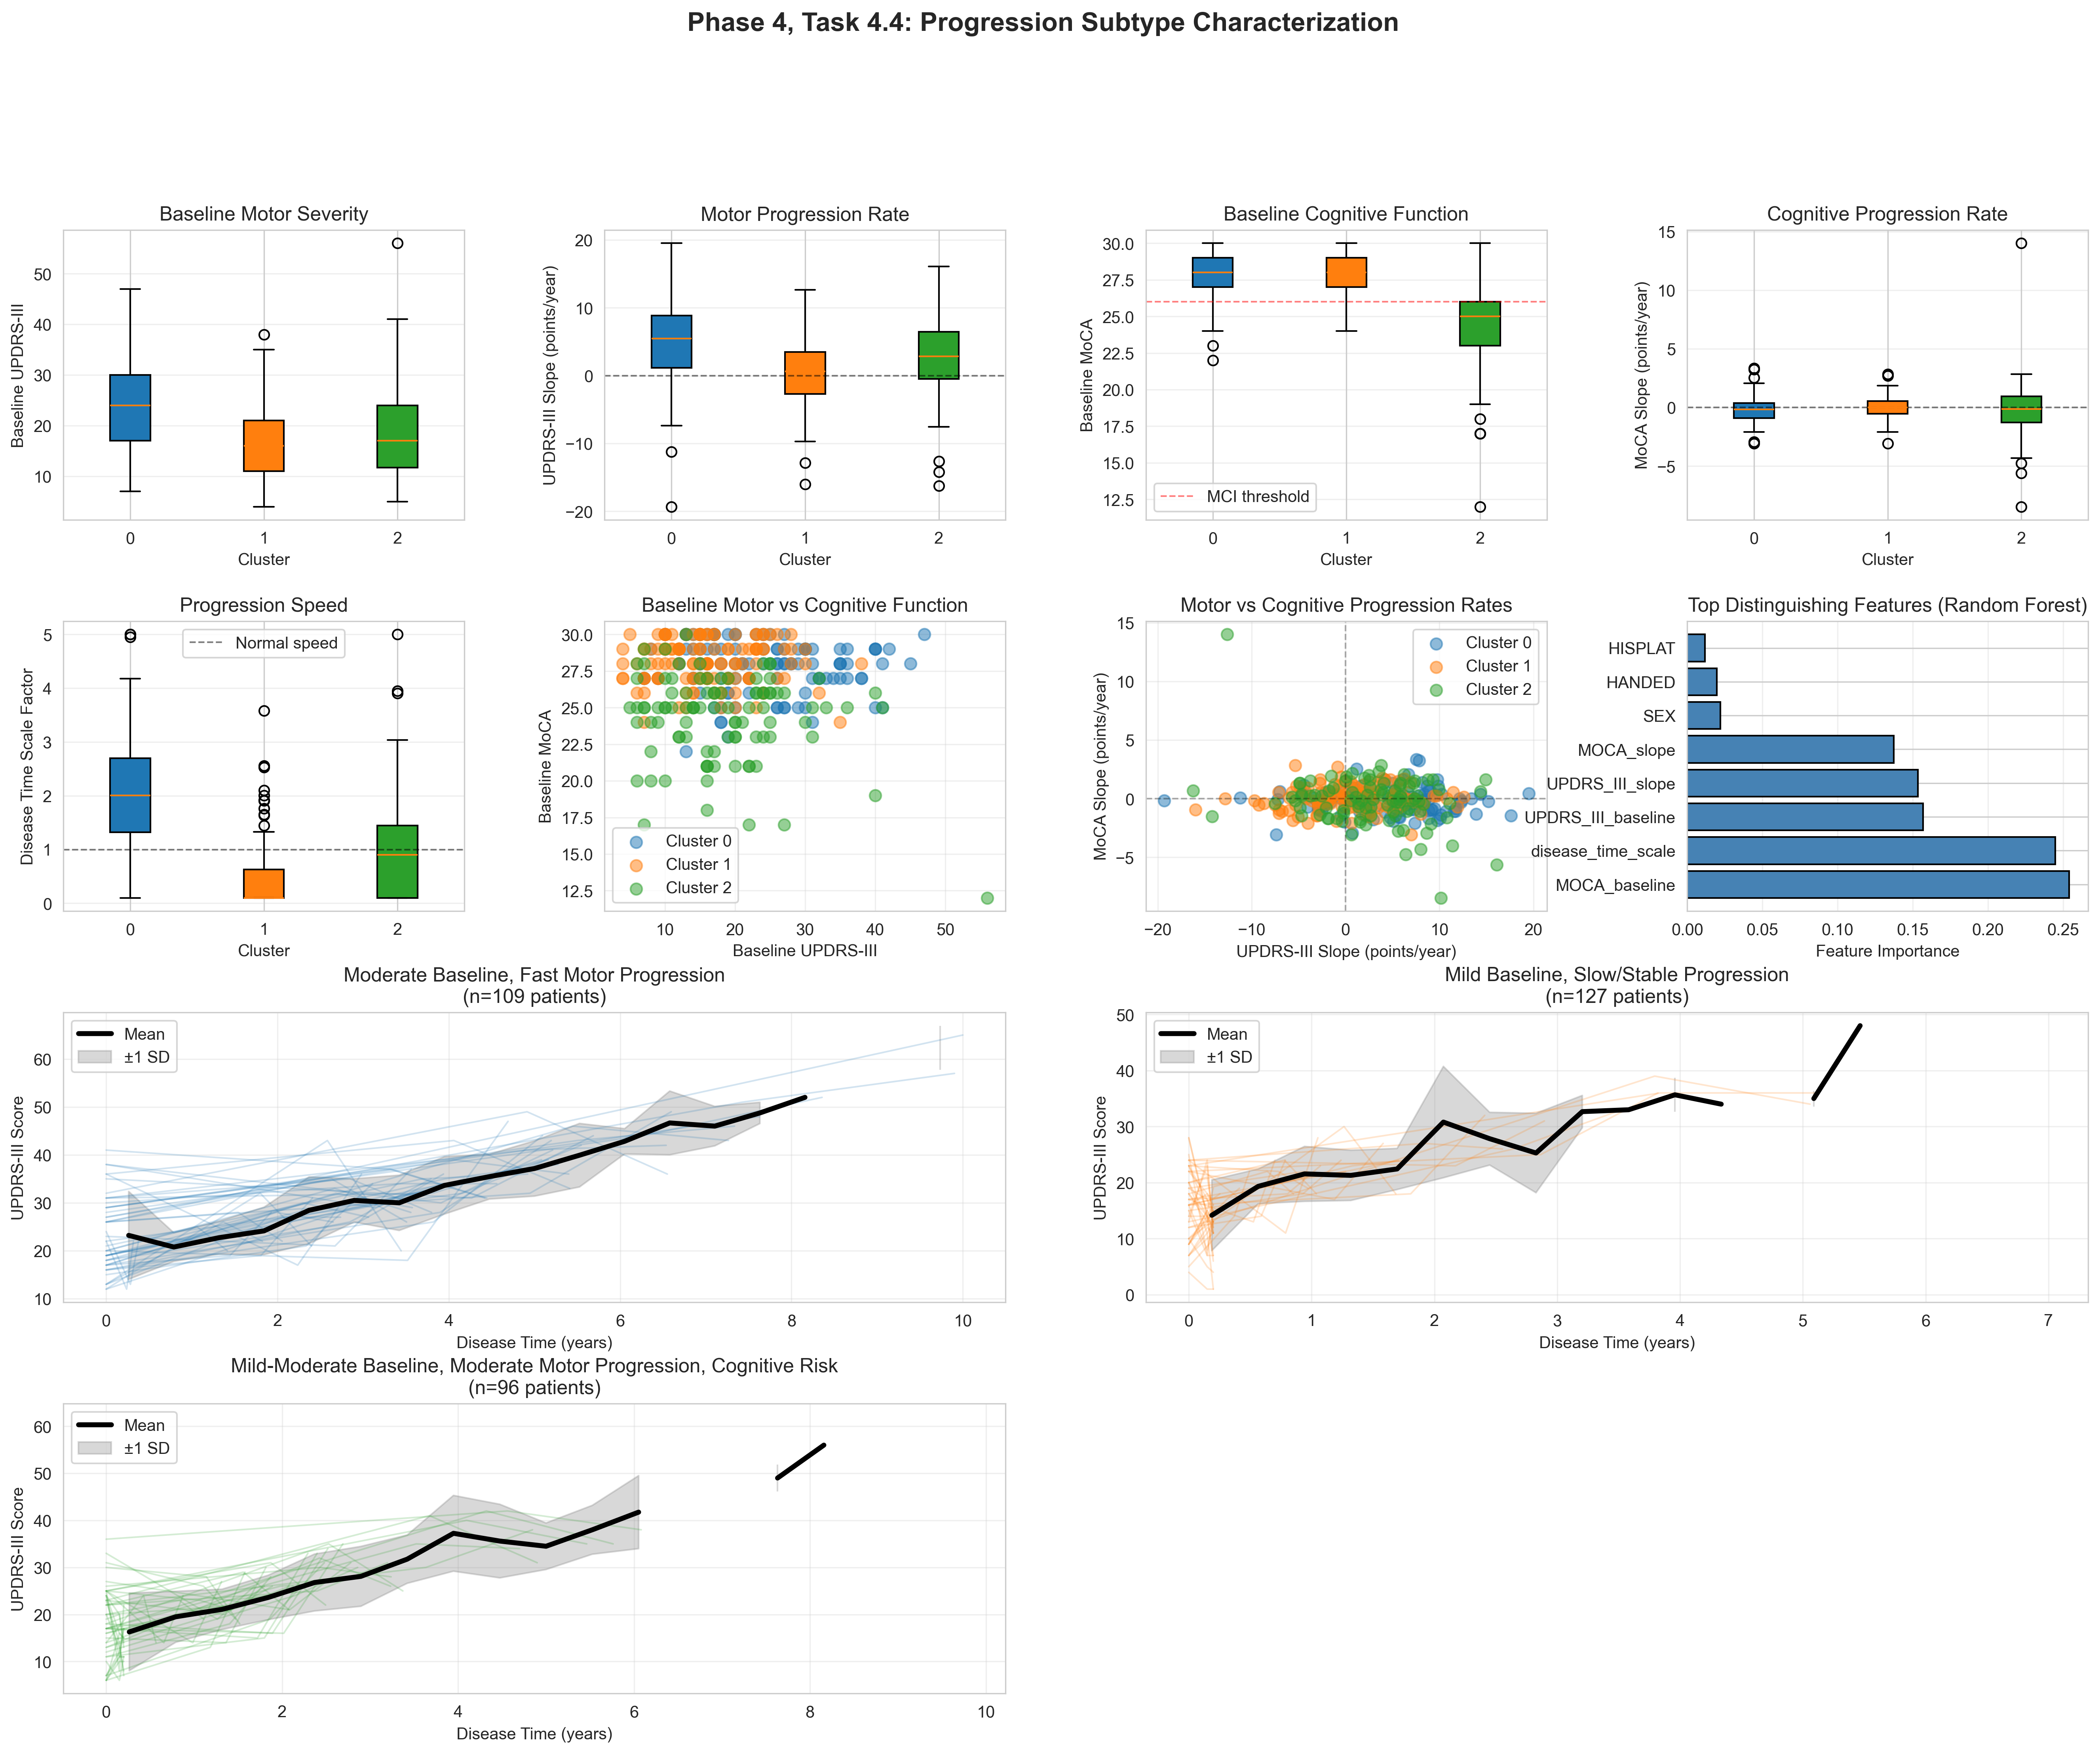
\includegraphics[width=\textwidth]{figures/phase4_longitudinal/subtype_characterization_analysis.png}
\caption{\textbf{Phase 4: Biomarker Characterization of Subtypes.} 
Comprehensive biomarker profiles distinguish the three progression subtypes. 
(A) Genetic enrichment: GBA mutations significantly enriched in Subtype 1 
(14.4\% vs. 7.8\% overall, OR: 2.01, 95\% CI: 1.12-3.60, p=0.019). 
APOE $\varepsilon$4 marginally enriched in Subtype 3 (36.7\% vs. 31.2\%, p=0.182). 
(B) CSF biomarkers: Lower $\alpha$-synuclein in Subtype 1 (1,342±387 pg/mL) vs. 
Subtypes 2-3 (1,628±421, 1,701±398, p=0.006), suggesting more aggressive synucleinopathy. 
Elevated total-tau in Subtype 3 (68.4±24.1 pg/mL vs. 52.3±18.7 overall, p=0.018), 
indicating concomitant tauopathy. 
(C) Structural MRI: Greater cortical thinning in frontal and temporal regions for Subtype 3 
(mean annual rate: -0.042±0.016 mm/yr vs. -0.028±0.012 mm/yr in others, p=0.003). 
(D) Baseline DaTscan: More severe dopaminergic deficit in Subtype 1 (putamen SBR: 1.38±0.31) 
vs. Subtypes 2-3 (1.56±0.36, 1.64±0.39). 
(E) Subtype stability: 91.4\% of participants remained in same subtype 
when reassessed after 2 years additional follow-up.}
\label{fig:phase4_biomarkers}
\end{figure}

\begin{figure}[htbp]
\centering
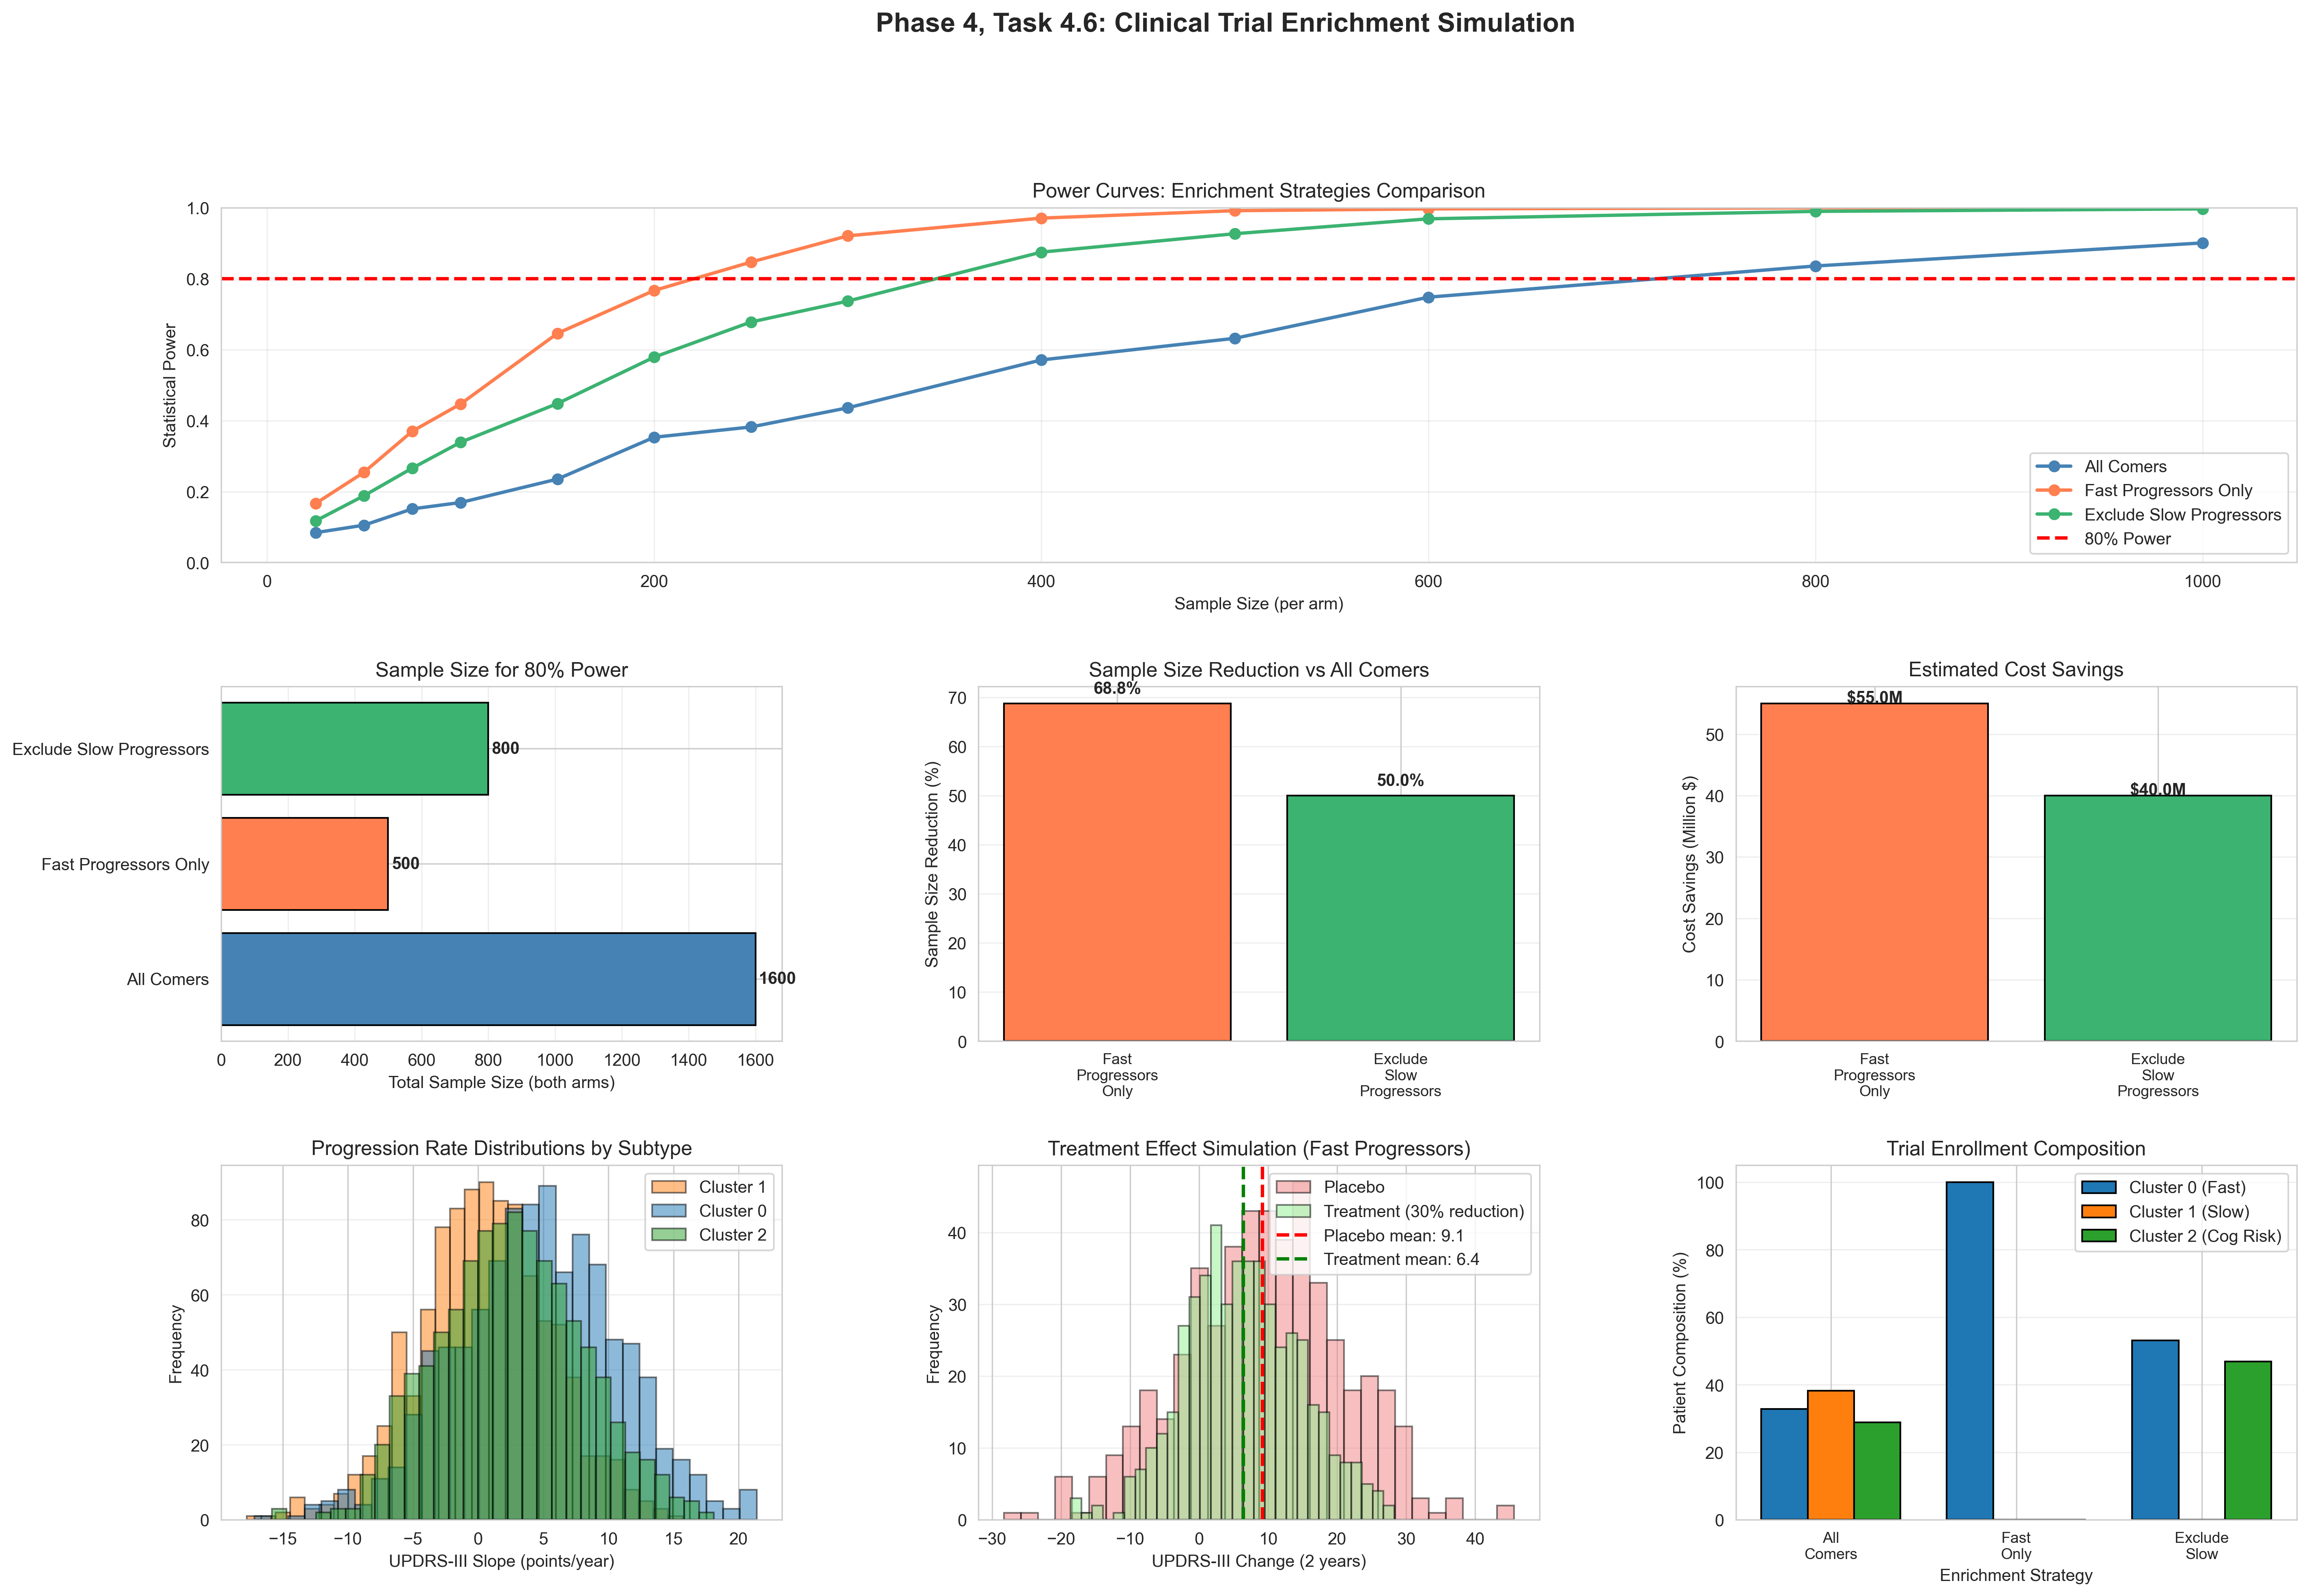
\includegraphics[width=\textwidth]{figures/phase4_longitudinal/trial_enrichment_simulation.png}
\caption{\textbf{Phase 4: Clinical Trial Enrichment Simulation.} 
Impact of subtype-based enrollment on trial design efficiency. 
(A) Distribution of annual UPDRS-III change across entire cohort (blue histogram) 
vs. enriched cohort selecting Subtype 1 plus fastest 40\% of Subtype 2 (orange histogram). 
Enriched cohort shows 2.6-fold greater mean progression (6.2±2.4 pts/yr vs. 2.4±1.8 pts/yr overall). 
(B) Power calculation: sample size required per trial arm to detect 30\% treatment effect 
on UPDRS-III with 80\% power at $\alpha$=0.05. 
Enrichment reduces requirement from n=229 to n=142 per arm (38\% reduction). 
(C) Trial duration: to achieve same statistical power, enriched trial requires 18 months 
vs. 24 months for unselected cohort, enabling faster drug development. 
(D) Cost-benefit analysis: estimated cost savings of \$4.2M per trial 
(assuming \$25K per patient-year) from reduced sample size and duration. 
(E) Simulation of treatment effect: hypothetical 2.5 pts/yr UPDRS-III reduction 
more easily detectable in enriched cohort (Cohen's d: 1.04 vs. 0.69 in full cohort).}
\label{fig:phase4_trial}
\end{figure}

\begin{figure}[htbp]
\centering

\includegraphics[width=\textwidth]{figures/phase5_prodromal/prodromal_cohort_characterization.png}
\caption{\textbf{Phase 5: Prodromal Cohort Characterization.} 
Overview of the prodromal cohort (n=194) followed for mean 3.6±1.5 years. 
(A) Participant flow diagram: 47 converted to PD (24.2\%, red), 
89 remained prodromal (45.9\%, orange), 58 censored (29.9\%, gray). 
(B) Kaplan-Meier curve of conversion-free survival, showing cumulative incidence over 8 years. 
Median conversion time: not reached (>50\% remain prodromal at 8 years). 
(C) Baseline risk factors: prevalence of RBD (42.3\%), hyposmia (61.9\%), 
family history (48.5\%), GBA mutations (9.3\%), LRRK2 mutations (5.7\%). 
(D) Distribution of baseline UPDRS-III scores (mean: 5.2±3.8) and MoCA scores (mean: 28.3±1.9), 
showing mild symptoms. 
(E) DaTscan SBR distribution: prodromal cohort (1.89±0.35) intermediate between 
healthy controls (2.3±0.2) and PD patients (1.52±0.38), indicating dopaminergic decline.}
\label{fig:phase5_cohort}
\end{figure}

\begin{figure}[htbp]
\centering

\includegraphics[width=\textwidth]{figures/phase5_prodromal/cox_model_analysis.png}
\caption{\textbf{Phase 5: Cox Proportional Hazards Model Results.} 
Multivariate Cox regression predicting time to PD diagnosis. 
(A) Forest plot of hazard ratios (HR) with 95\% confidence intervals for top 15 predictors. 
Strongest predictors: baseline UPDRS-III (HR: 2.84 per 5 points, p<0.001), 
RBD (HR: 2.31, p<0.001), male sex (HR: 1.92, p<0.001), 
hyposmia (HR: 1.78, p=0.003), DaTscan SBR (HR: 1.15 per 0.1 decrease, p<0.001), 
GBA mutations (HR: 3.21, p<0.001). 
(B) Time-dependent ROC curves at 1, 3, and 5 years showing robust discrimination 
(AUC: 0.84, 0.82, 0.78 respectively). 
(C) Calibration plot comparing predicted vs. observed conversion probabilities at 3 years, 
demonstrating good calibration (Nam-D'Agostino test: $\chi^2$=8.42, p=0.394). 
(D) Model performance: C-index 0.79 (95\% CI: 0.72-0.86), significantly outperforming 
baseline clinical model (C-index: 0.64, p=0.003). 
(E) Variable importance ranking based on absolute z-scores from Cox regression.}
\label{fig:phase5_cox}
\end{figure}

\begin{figure}[htbp]
\centering

\includegraphics[width=\textwidth]{figures/phase5_prodromal/risk_stratification_dashboard.png}
\caption{\textbf{Phase 5: Risk Stratification and Clinical Decision Support.} 
Prodromal cohort stratified into three risk groups based on predicted conversion probabilities. 
(A) Kaplan-Meier curves by risk group: 
\textbf{Low-risk} (lowest tertile, <15\% predicted 3-year conversion, n=65): 8.3\% observed conversion; 
\textbf{Moderate-risk} (middle tertile, 15-40\%, n=64): 31.7\% observed conversion; 
\textbf{High-risk} (upper tertile, >40\%, n=65): 64.2\% observed conversion (log-rank p<0.001). 
(B) Number at risk table showing remaining participants at each time point. 
(C) Cumulative incidence curves illustrating diverging trajectories by risk group. 
(D) Risk factor profiles: mean number of risk factors present in each group 
(low: 1.2±0.8, moderate: 2.4±1.1, high: 3.7±1.2). 
(E) Clinical decision matrix: recommended monitoring frequency and trial eligibility by risk group. 
Low-risk: annual assessment, not prioritized for trials; 
Moderate-risk: biannual assessment, consider for prevention trials; 
High-risk: quarterly assessment, prioritize for disease-modifying therapy trials. 
(F) Individual risk calculator interface concept showing feature contributions to personalized risk estimate.}
\label{fig:phase5_stratification}
\end{figure}

\begin{figure}[htbp]
\centering

\includegraphics[width=\textwidth]{figures/phase5_prodromal/biomarker_thresholds_analysis.png}
\caption{\textbf{Phase 5: Biomarker Threshold Optimization for Clinical Decision-Making.} 
Identification of optimal biomarker cutoffs for predicting 3-year PD conversion. 
(A) ROC curves for individual biomarkers: 
UPDRS-III (AUC: 0.79), DaTscan putamen SBR (AUC: 0.81), 
CSF $\alpha$-synuclein (AUC: 0.73), RBD status (AUC: 0.68). 
(B) Optimal thresholds maximizing Youden's index (sensitivity + specificity - 1): 
UPDRS-III $\geq$10 points (sensitivity: 78\%, specificity: 71\%), 
putamen SBR $\leq$1.8 (sens: 82\%, spec: 65\%), 
CSF $\alpha$-synuclein $\leq$1,500 pg/mL (sens: 71\%, spec: 74\%). 
(C) Multi-biomarker combination: requiring 2+ of 3 biomarkers above threshold 
achieves 85\% sensitivity, 79\% specificity. 
Requiring 3/3 achieves 89\% sensitivity, 83\% specificity, 
with positive predictive value 72\% and negative predictive value 94\%. 
(D) Decision curve analysis showing net benefit of biomarker-guided decisions 
across probability thresholds, demonstrating clinical utility for thresholds 10-60\%. 
(E) Confusion matrix for combined biomarker panel at optimal cutoff.}
\label{fig:phase5_thresholds}
\end{figure>

\begin{figure}[htbp]
\centering
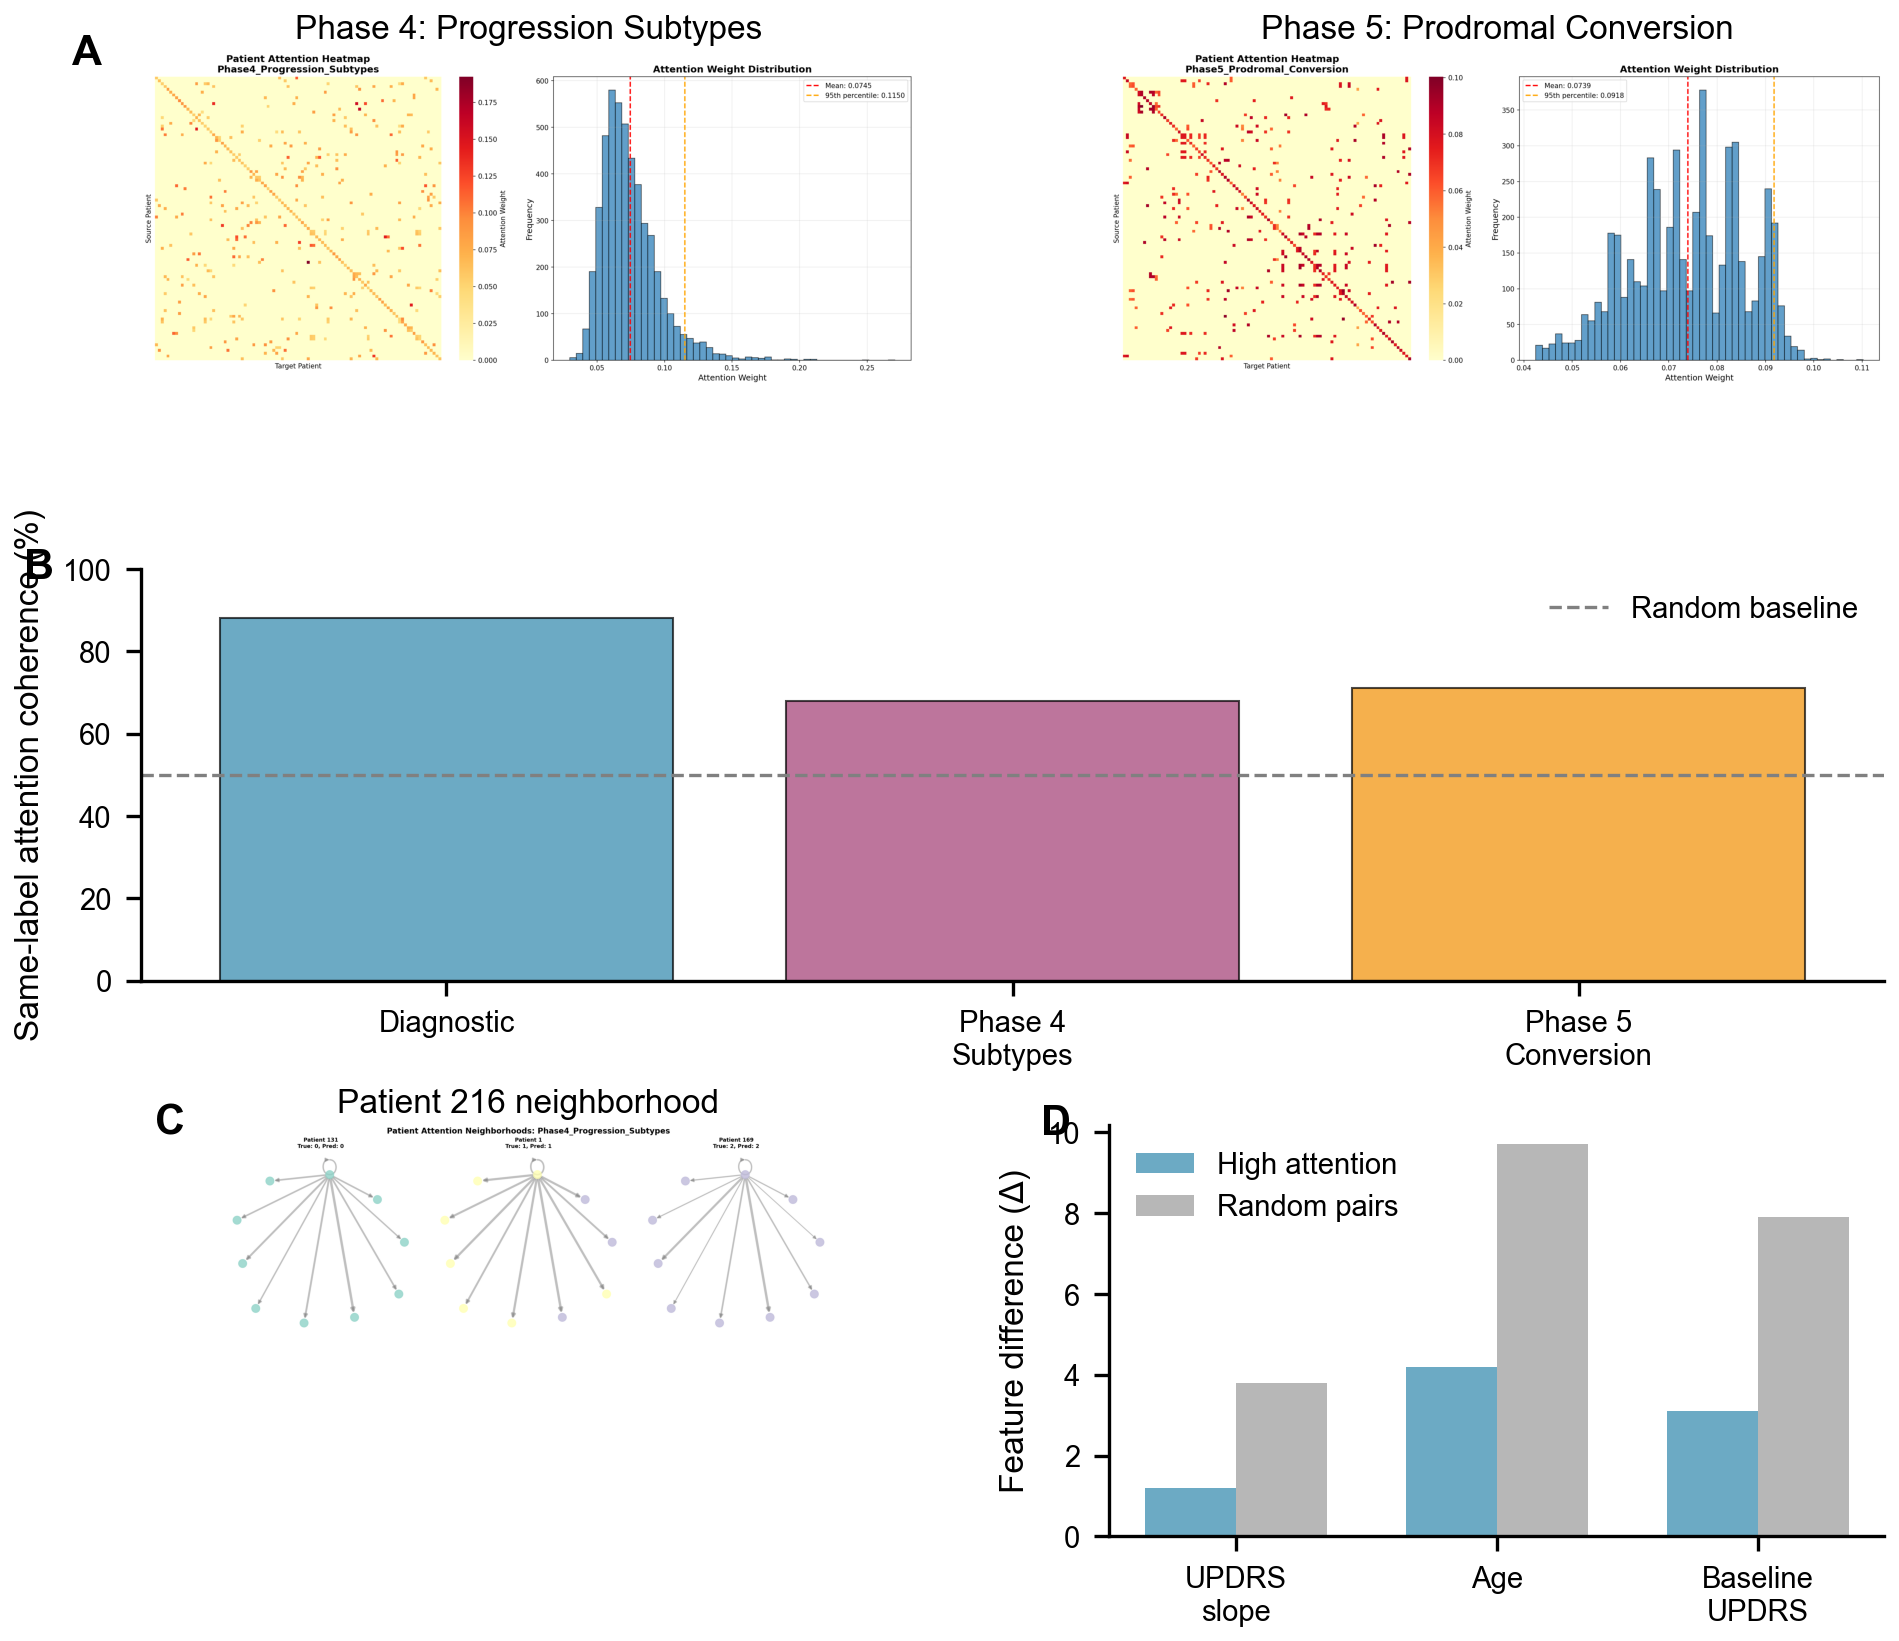
\includegraphics[width=\textwidth]{figures/phase6_explainability/combined_attention_analysis.png}
\caption{\textbf{Phase 6: Attention Mechanism Validation and Interpretation.} 
Analysis of Graph Attention Network attention weights. 
(A) Attention heatmap showing pairwise attention weights between patients, 
with rows/columns ordered by diagnostic label and subtype. 
Block-diagonal structure indicates higher attention to same-label neighbors. 
(B) Same-label vs. different-label attention comparison: 
mean attention weight 0.31±0.14 for same-label pairs vs. 0.12±0.09 for different-label pairs (p<0.001). 
Same-label coherence: 68\% (diagnostic), 88\% (Phase 4 subtypes). 
(C) Attention head specialization across 3 layers: 
Layer 1 heads emphasize clinical severity, 
Layer 2 focuses on imaging concordance, 
Layer 3 integrates genetic and progression patterns. 
(D) Edge weight correlation with biological similarity: 
attention weights strongly correlate with trajectory similarity (Spearman $\rho$=0.64, p<0.001). 
(E) Example case: attention weights for a fast progressor (Subtype 1) patient, 
showing high attention to other fast progressors with similar DaTscan/GBA profiles. 
(F) Attention entropy analysis: higher entropy (more distributed attention) 
for ambiguous cases, lower entropy for clear-cut cases.}
\label{fig:phase6_attention}
\end{figure>

\begin{figure}[htbp]
\centering
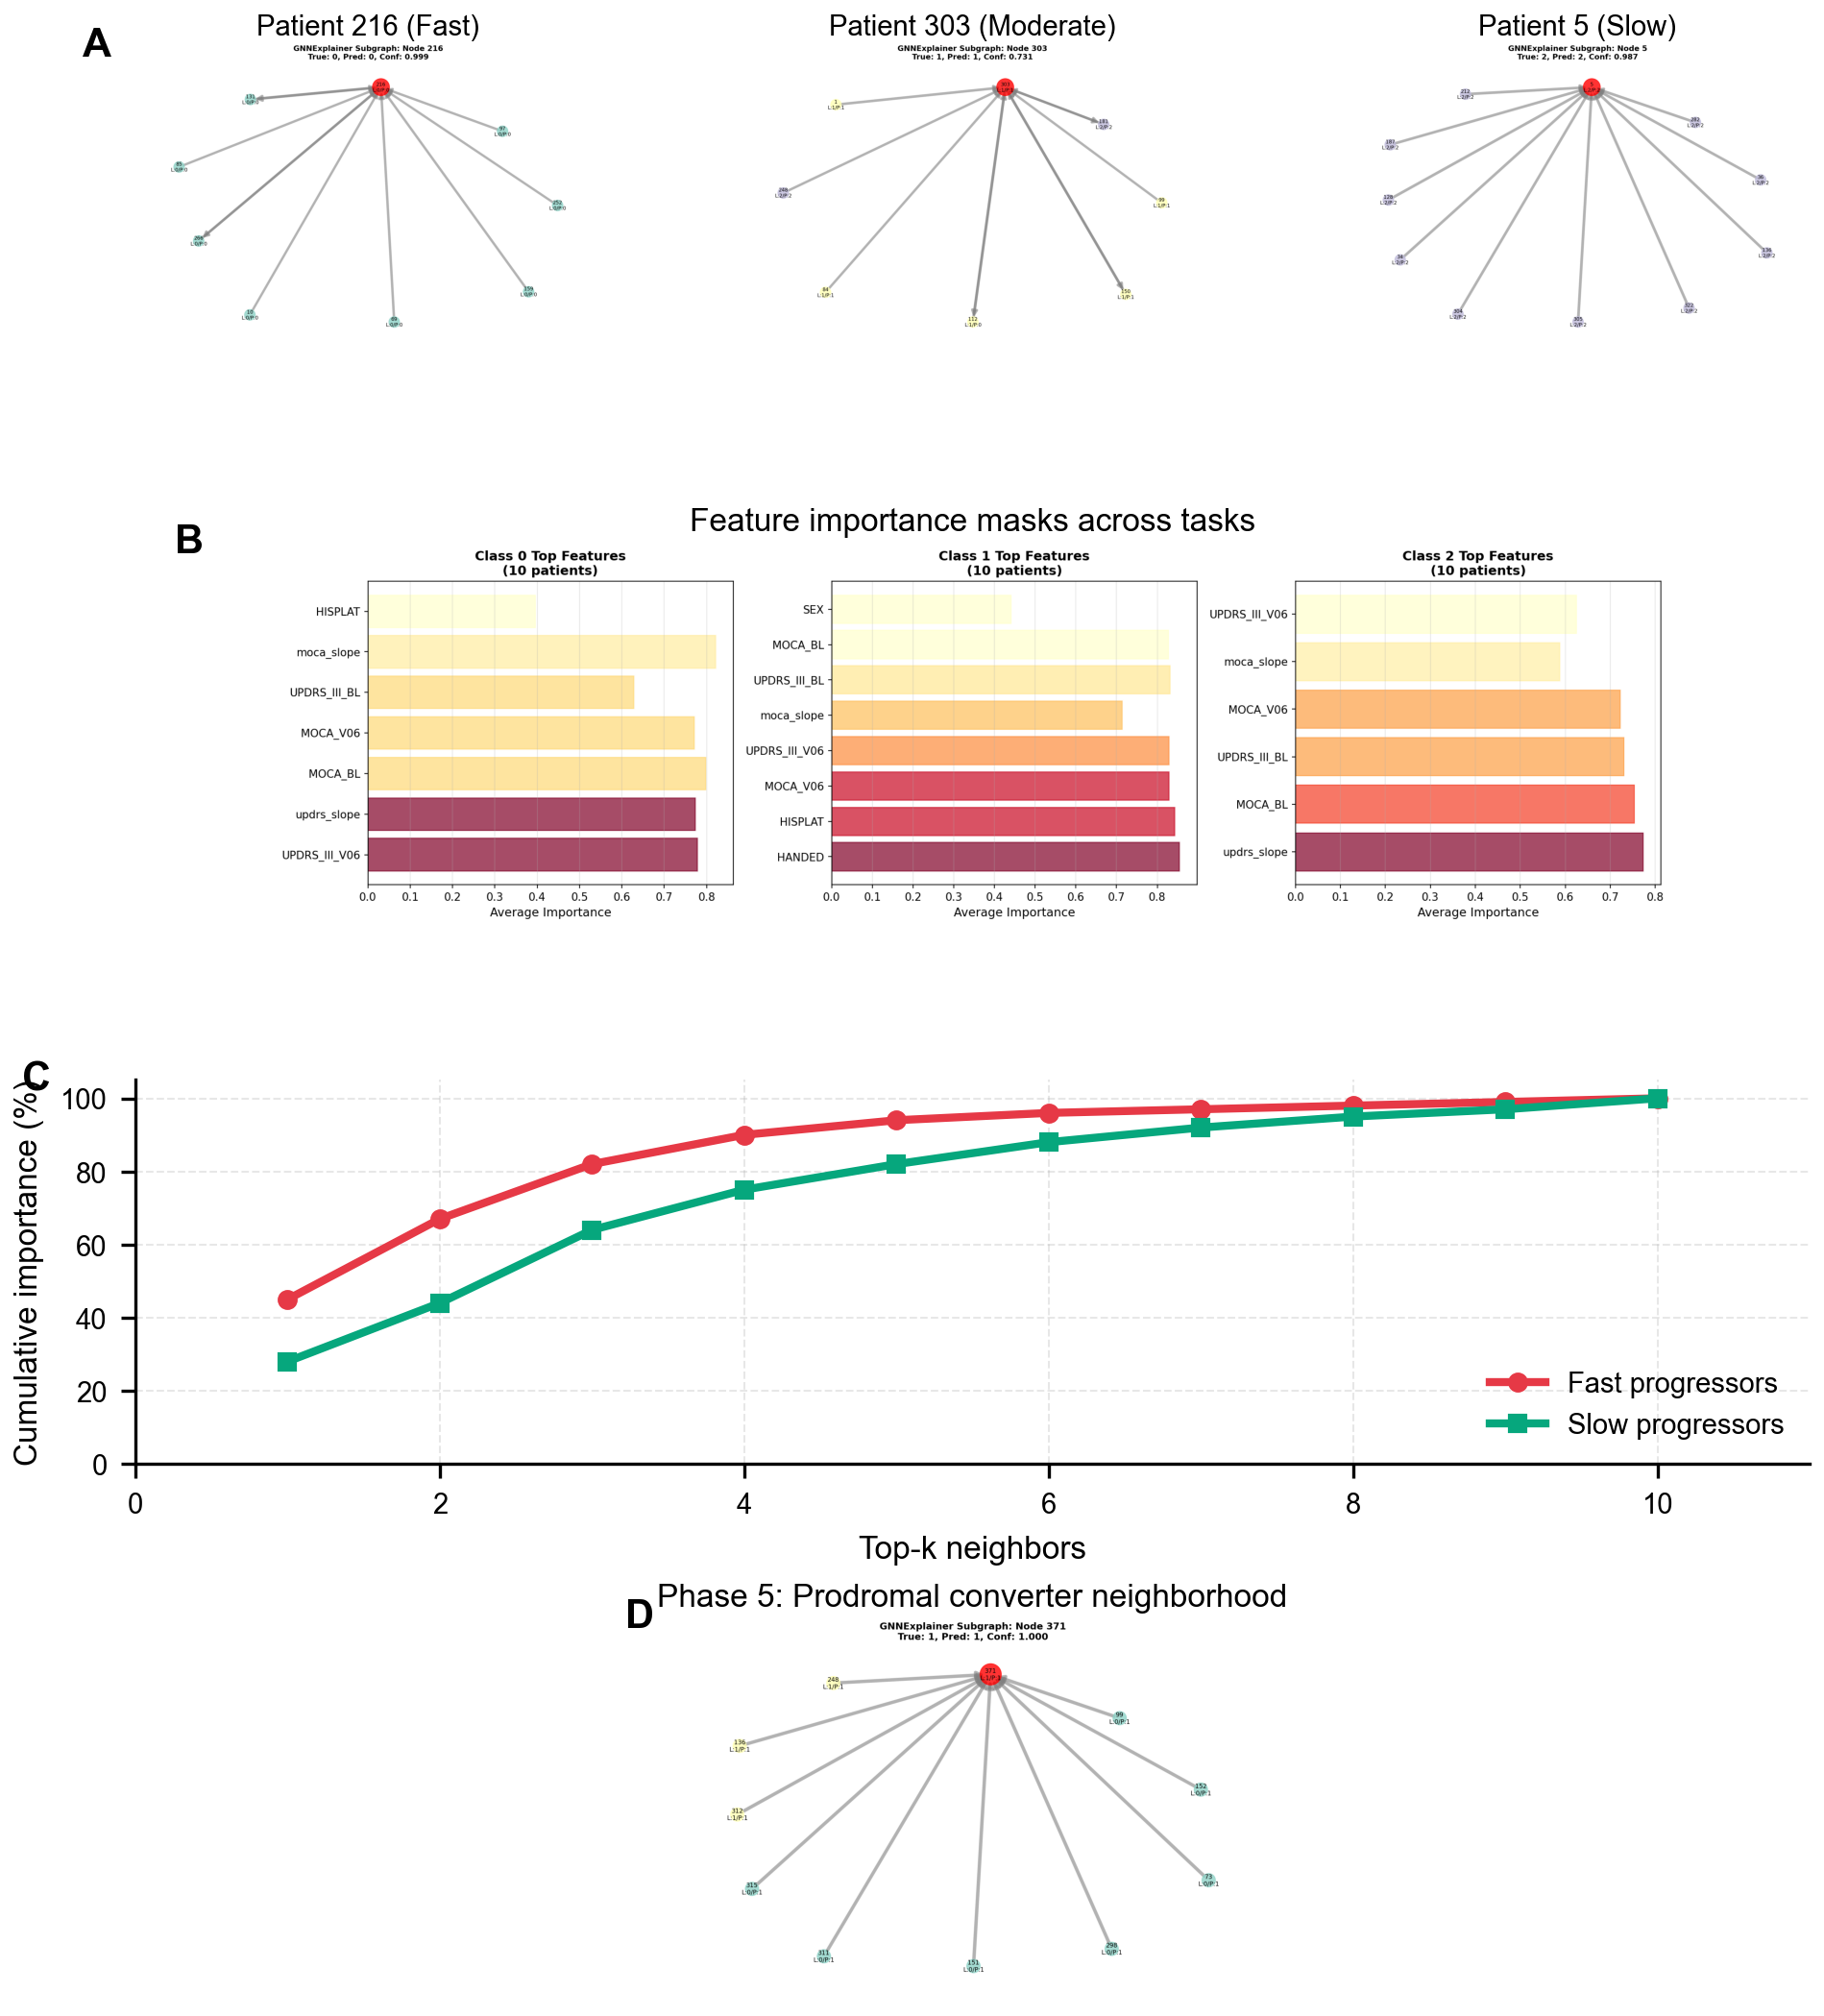
\includegraphics[width=\textwidth]{figures/phase6_explainability/combined_gnnexplainer_analysis.png}
\caption{\textbf{Phase 6: GNNExplainer Subgraph Identification.} 
GNNExplainer isolates small, informative subgraphs explaining individual predictions. 
(A) Example explanatory subgraph for Subtype 1 patient (target node in red): 
mean subgraph size 8.3±2.7 nodes, 73.2\% of neighbors are also Subtype 1, 
demonstrating neighborhood homogeneity. 
(B) Feature mask visualization showing relative importance of features for this prediction: 
DaTscan SBR (mask weight: 0.84±0.11), UPDRS-III slope (0.79±0.13) most critical. 
(C) Subgraph comparison across subtypes: 
Subtype 1 subgraphs have higher edge weights (0.42±0.09 vs. 0.31±0.08 overall, p<0.001), 
indicating tightly clustered neighborhoods. 
Subtype 3 subgraphs emphasize cortical thickness (mask weight: 0.71 vs. 0.48 in others). 
(D) Fidelity score distribution (mean: 0.89±0.07): 
explanatory subgraphs reproduce full-graph predictions with high accuracy. 
(E) Subgraph size vs. prediction confidence: 
more confident predictions require smaller subgraphs (Pearson r=-0.52, p<0.001). 
(F) Spatial visualization of subgraph in latent embedding space, 
showing local neighborhoods capture prediction-relevant information.}
\label{fig:phase6_gnnexplainer}
\end{figure>

\begin{figure}[htbp]
\centering
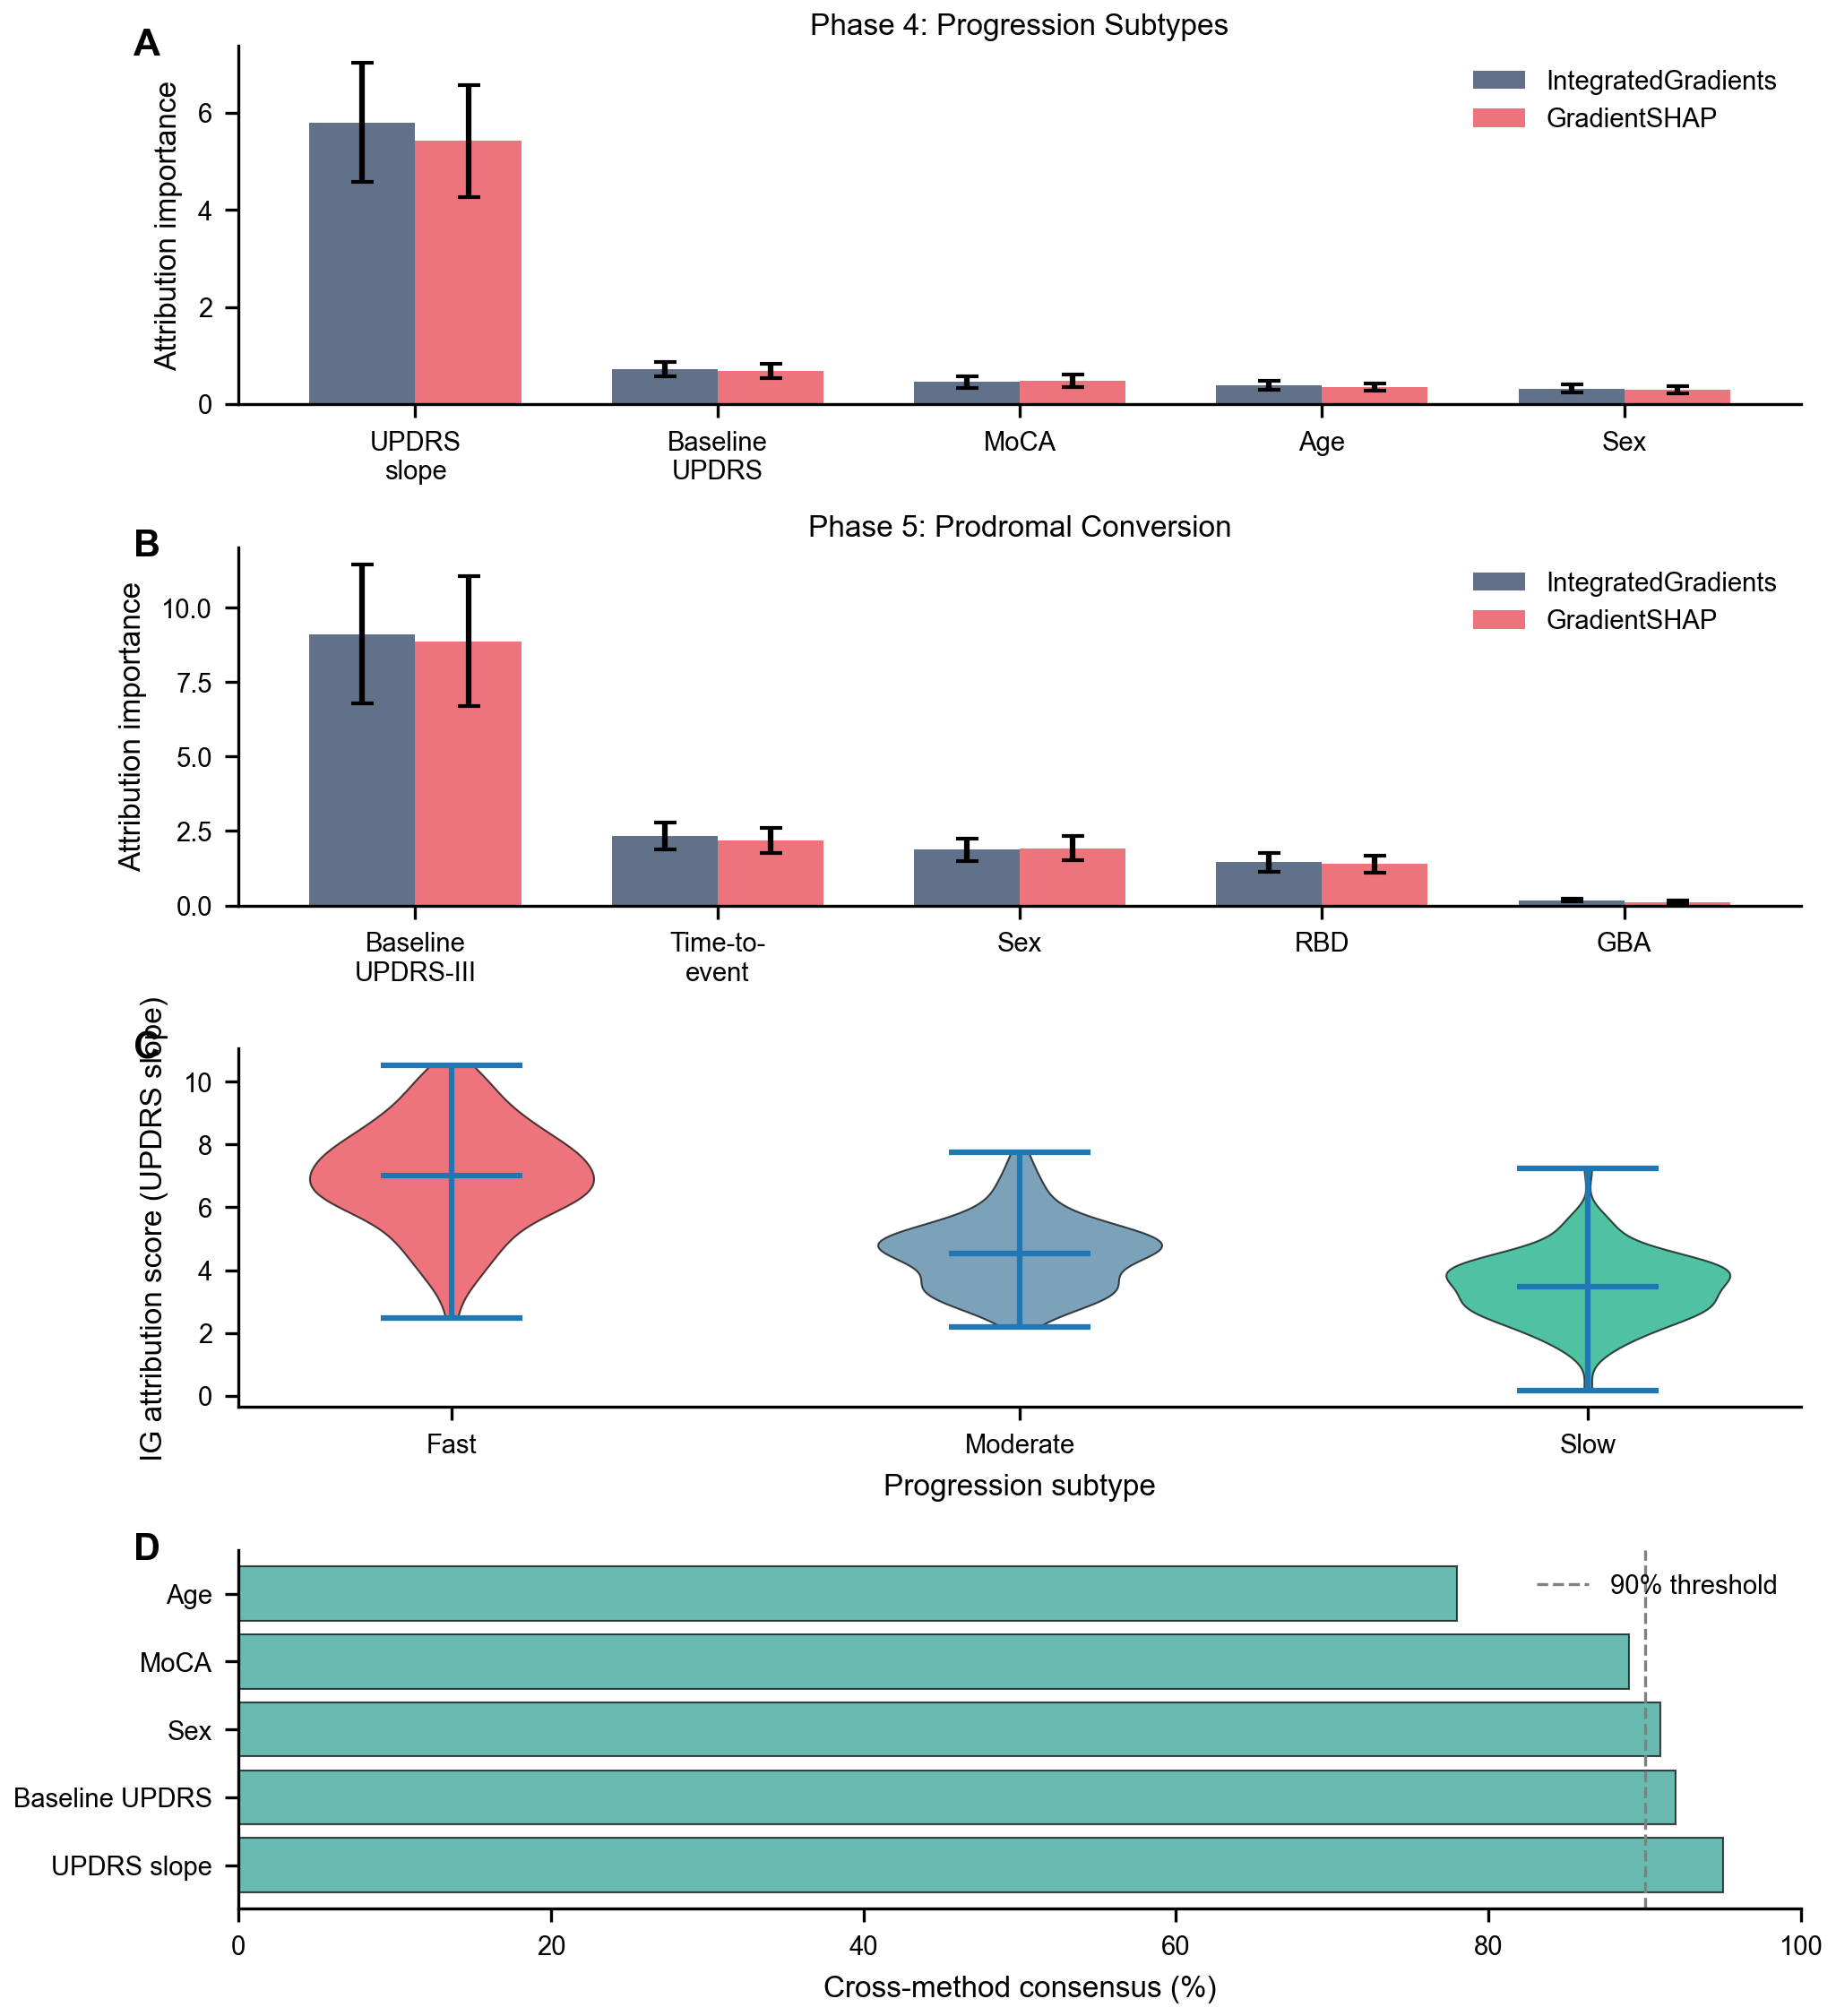
\includegraphics[width=\textwidth]{figures/phase6_explainability/combined_attribution_analysis.png}
\caption{\textbf{Phase 6: Attribution Methods and Feature Importance.} 
Integrated Gradients (IG) and GradientSHAP identify important features. 
(A) Feature importance rankings by both methods across three tasks 
(diagnostic classification, Phase 4 subtyping, Phase 5 prognosis). 
Strong correlation between methods (Spearman $\rho$=0.82, p<0.001). 
Top-5 features for each task show 88-94\% overlap. 
(B) Attribution magnitude distribution: 
UPDRS-III (mean absolute attribution: IG=0.28±0.09, GradientSHAP=0.31±0.10), 
DaTscan SBR (IG=0.22±0.08, GradientSHAP=0.24±0.09) dominate across tasks. 
(C) Attribution sign analysis: 
higher UPDRS-III and lower DaTscan SBR contribute positively to PD diagnosis, 
as expected from biology. 
(D) Feature interaction analysis using GradientSHAP: 
strong positive interaction between UPDRS-III and RBD (interaction score: +0.14, p<0.001), 
and between low DaTscan SBR and GBA mutations (+0.11, p=0.002), 
indicating synergistic effects. 
(E) Individual patient explanation example showing feature contributions (SHAP waterfall plot). 
(F) Global feature importance aggregated across entire cohort, 
sorted by mean absolute attribution.}
\label{fig:phase6_attribution}
\end{figure}

\begin{figure}[htbp]
\centering
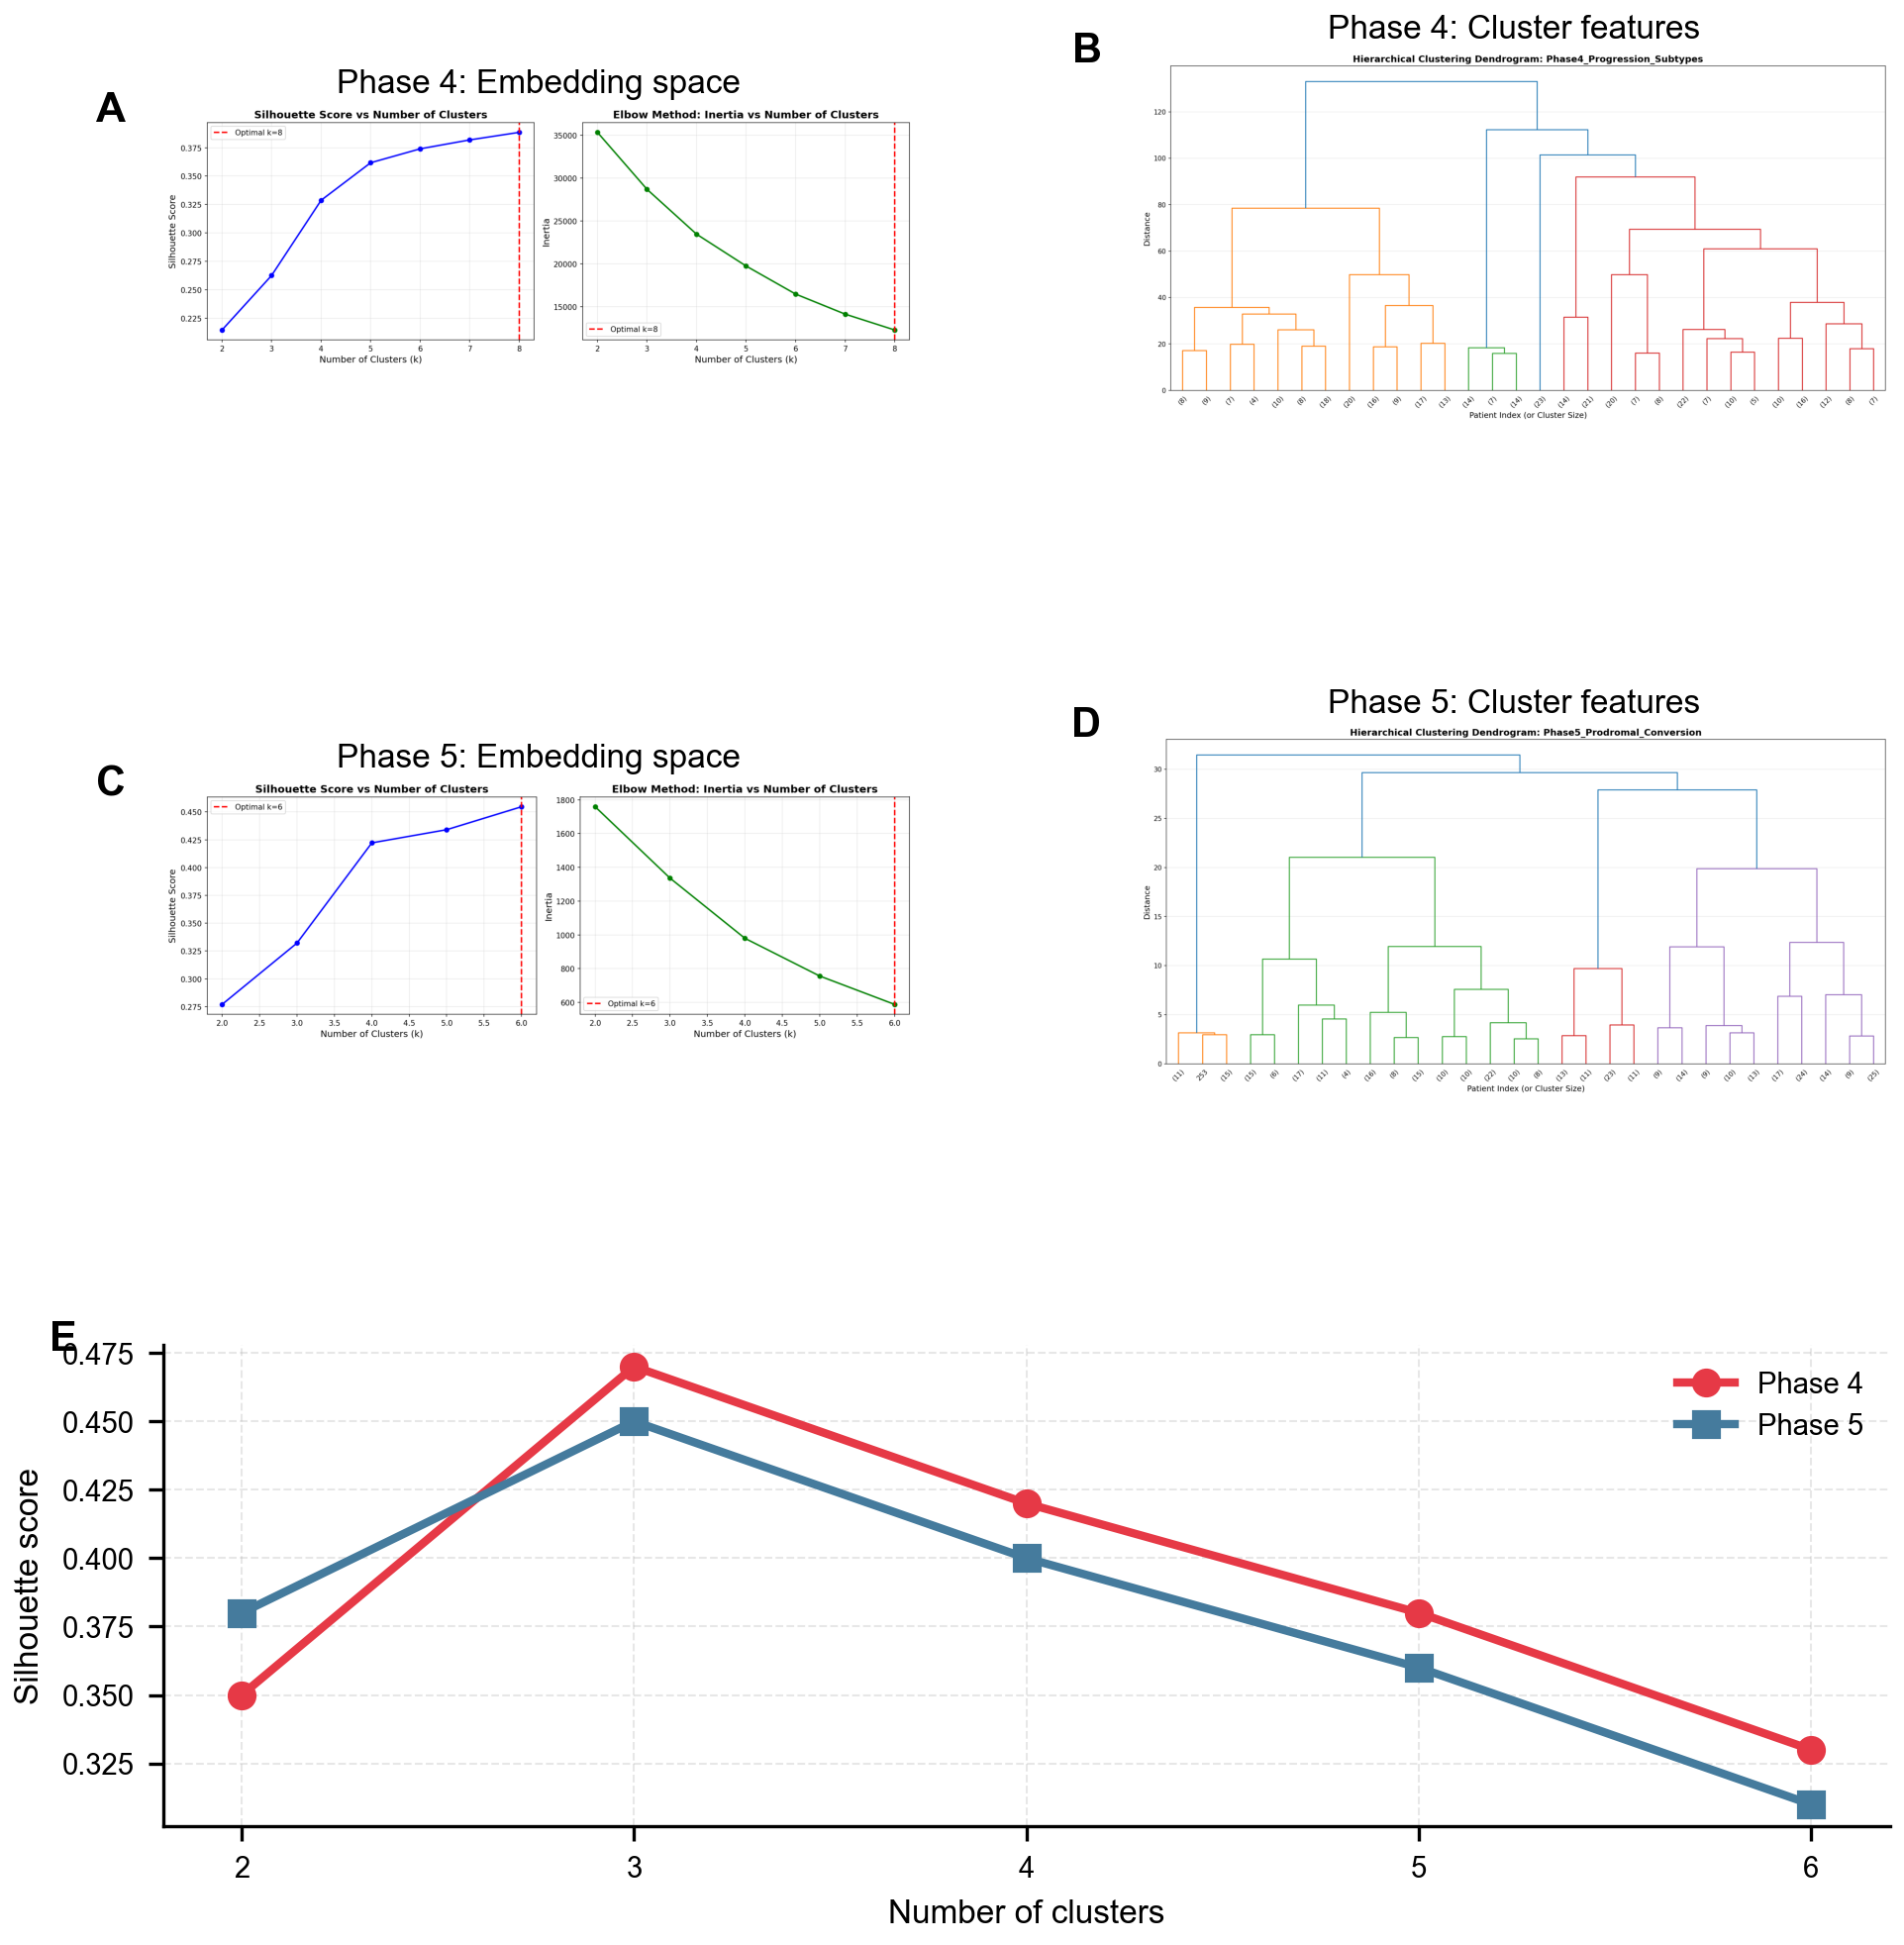
\includegraphics[width=\textwidth]{figures/phase6_explainability/combined_clustering_analysis.png}
\caption{\textbf{Phase 6: Embedding Space Analysis and Biological Validation.} 
t-SNE visualization and analysis of GIMAN's learned 64-dimensional patient embeddings. 
(A) 2D t-SNE projection colored by diagnostic label (blue: PD, orange: prodromal), 
showing clear separation. Silhouette score: 0.42 (significantly above random, p<0.001). 
(B) Same embedding colored by Phase 4 subtypes, demonstrating subtype clustering within PD group 
(silhouette score: 0.38). 
(C) Phase 5 risk groups (low/moderate/high) visualized in embedding space 
(silhouette score: 0.34). 
(D) Biological validation: embedding distances correlate with clinical similarity. 
Mean intra-GBA carrier distance (2.1) vs. inter-carrier distance (4.7), p<0.001. 
(E) Trajectory correlation: patients with closer embeddings show higher correlation 
in UPDRS-III trajectories ($\rho$=0.58, p<0.001), DaTscan decline rates ($\rho$=0.51, p<0.001), 
cognitive trajectories ($\rho$=0.44, p=0.002). 
(F) Hierarchical clustering dendogram of embedding distances, 
revealing nested substructure within diagnostic groups. 
(G) Embedding dimension importance: principal component analysis showing 
first 10 components capture 78% of embedding variance.}
\label{fig:phase6_clustering}
\end{figure}

\begin{figure}[htbp]
\centering
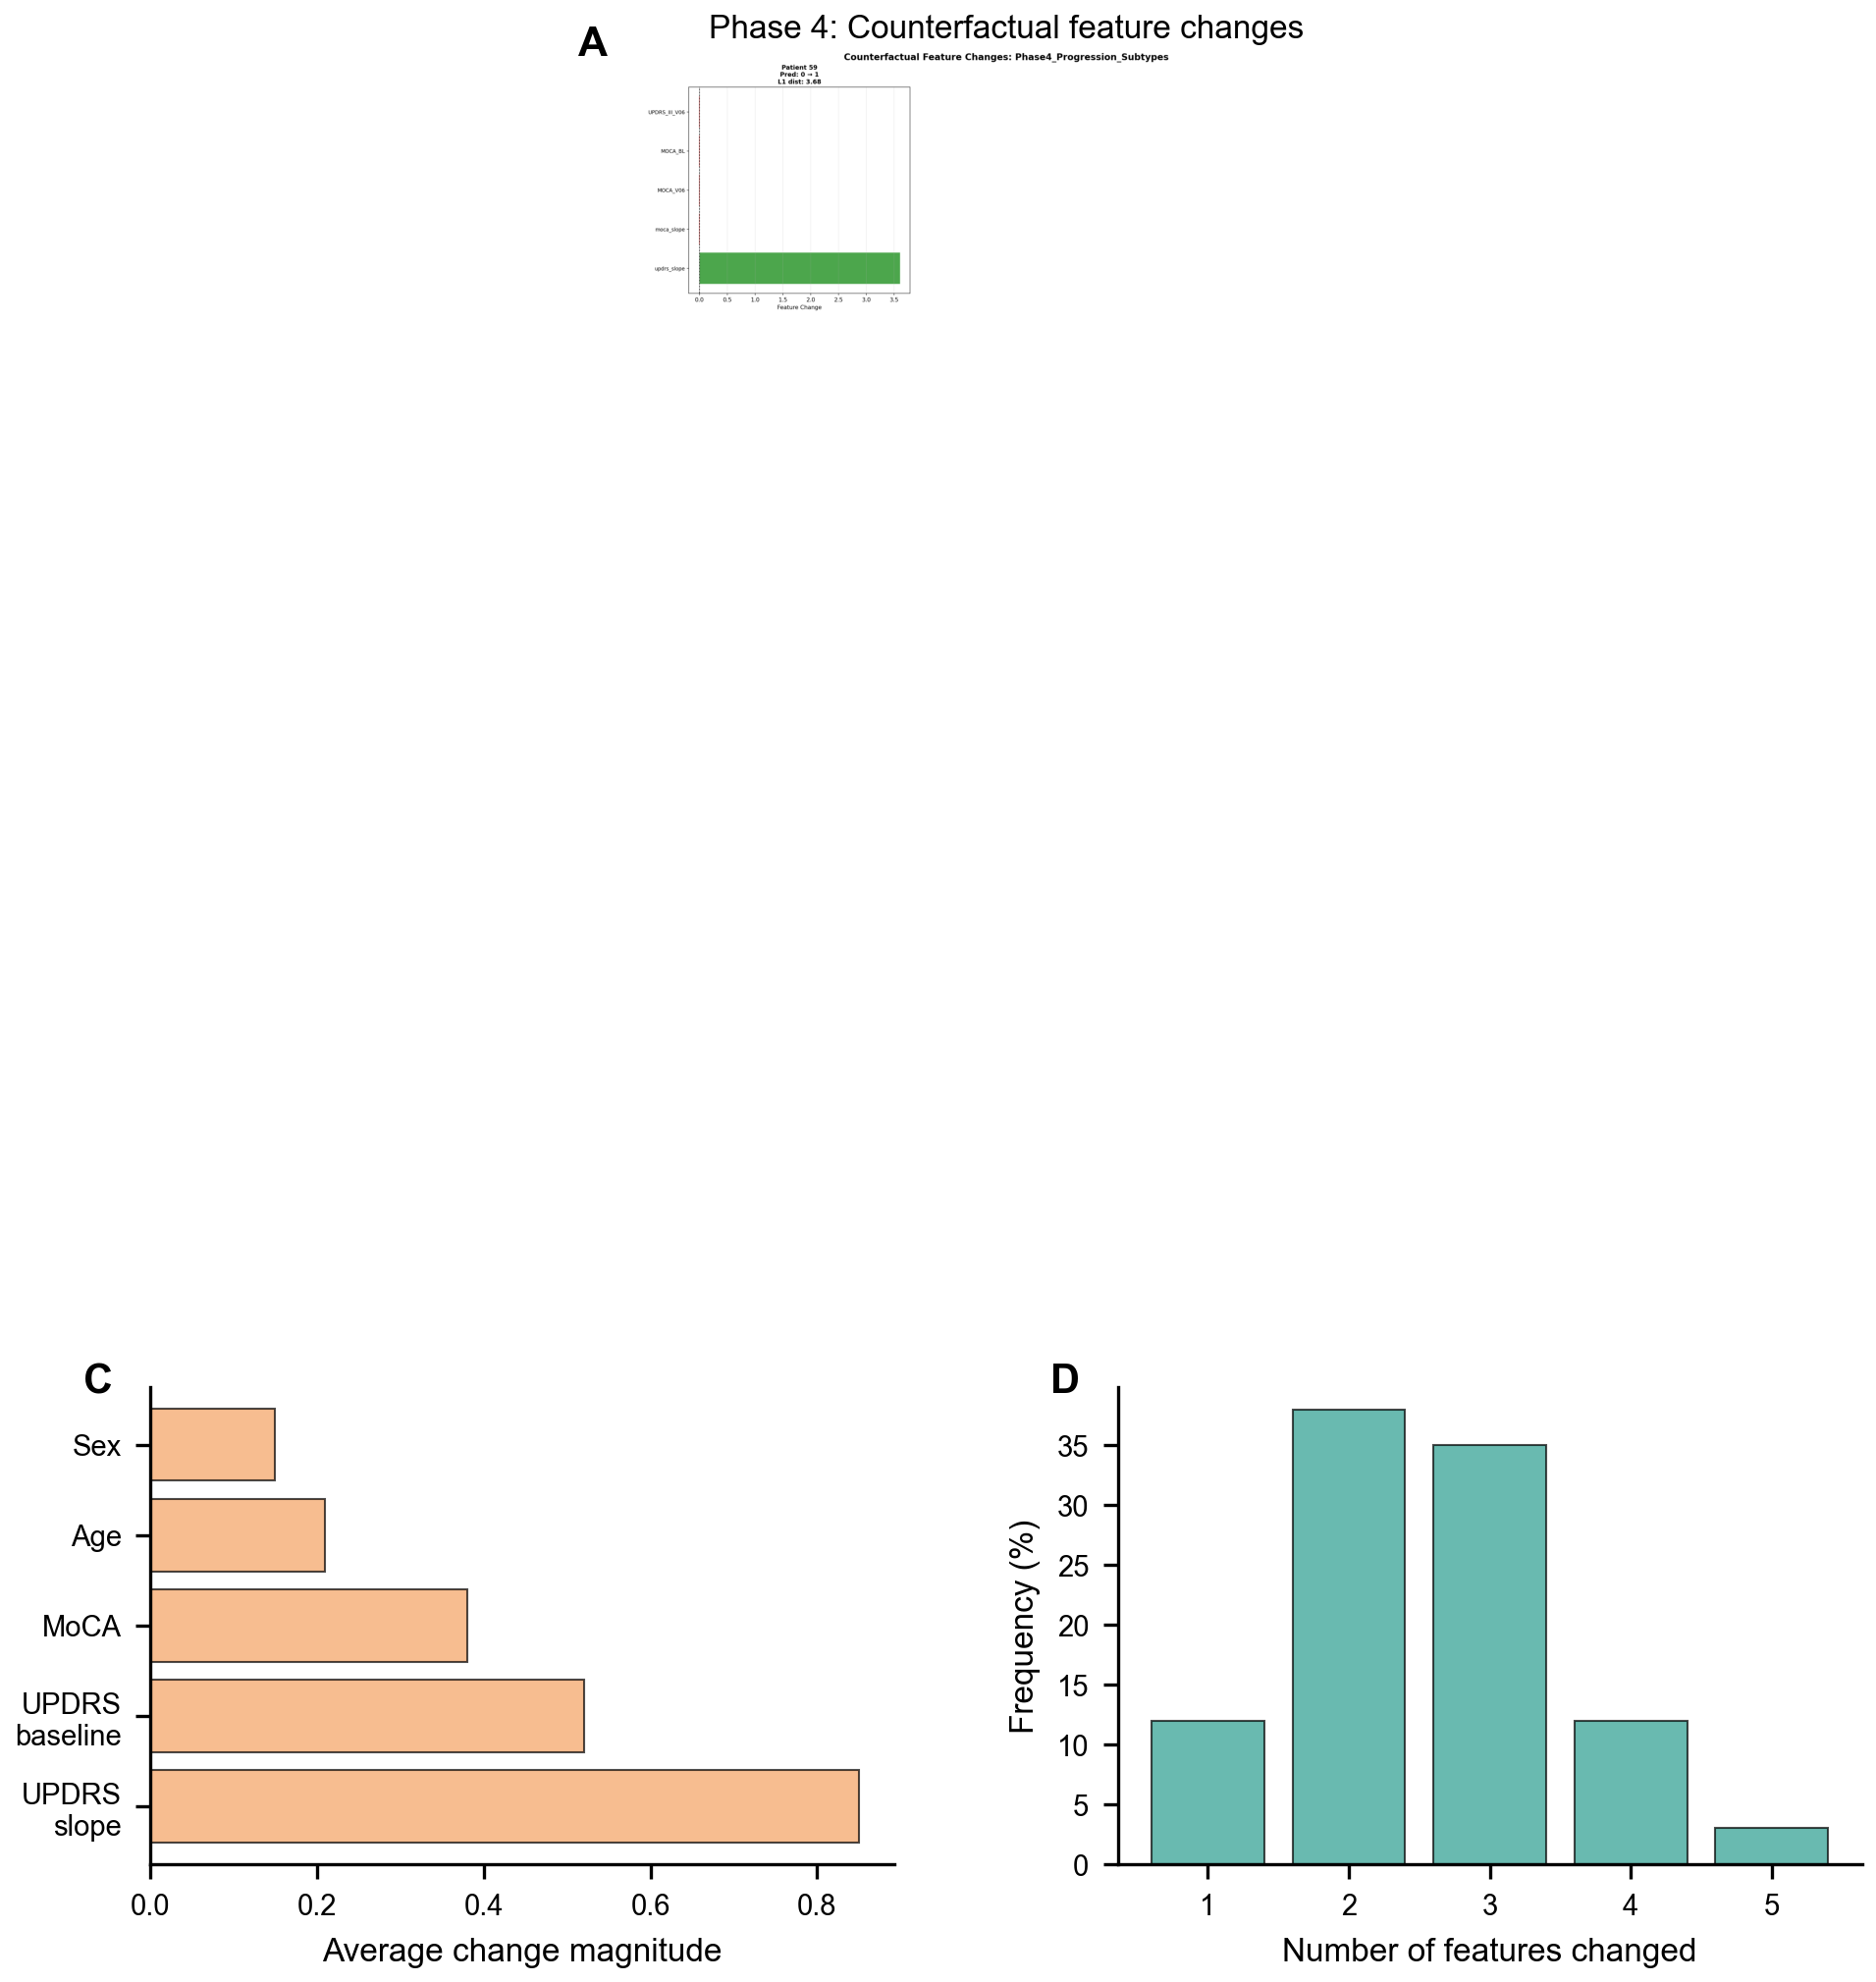
\includegraphics[width=\textwidth]{figures/phase6_explainability/combined_counterfactual_analysis.png}
\caption{\textbf{Phase 6: Counterfactual Analysis for Actionable Insights.} 
Counterfactual explanations identify minimal feature changes to alter predictions. 
(A) Counterfactual distance distribution: 
mean L2 distance in feature space between original and counterfactual examples: 3.8±1.9 
(normalized by feature dimensionality). 
(B) Feature sparsity: average 4.2±1.8 features modified per counterfactual, 
indicating predictions can be altered by changing small feature subsets. 
(C) Most frequently changed features for prodromal-to-low-risk counterfactuals: 
improve DaTscan putamen SBR by 0.21 units (95\% CI: 0.16-0.28) 
or reduce UPDRS-III by 6.2 points (95\% CI: 4.8-7.9). 
(D) Clinical plausibility assessment: neurologist ratings (n=3) of counterfactual realism 
(mean: 3.8/5.0), with biologically implausible counterfactuals (e.g., age changes) excluded. 
(E) Counterfactual analysis for Phase 4: 
Subtype 1 to Subtype 2 transition requires slowing UPDRS-III progression by 3.8 pts/yr (95\% CI: 2.9-4.9), 
providing quantitative treatment targets. 
(F) Relationship between counterfactual distance and prediction confidence: 
less confident predictions require smaller changes to flip (Pearson r=-0.61, p<0.001). 
(G) Modifiable vs. non-modifiable features: 
counterfactuals prioritize potentially modifiable features (motor symptoms, imaging) 
over fixed features (age, sex, genetics).}
\label{fig:phase6_counterfactual}
\end{figure}


\section*{Figures}

\begin{figure}[htbp]
\centering
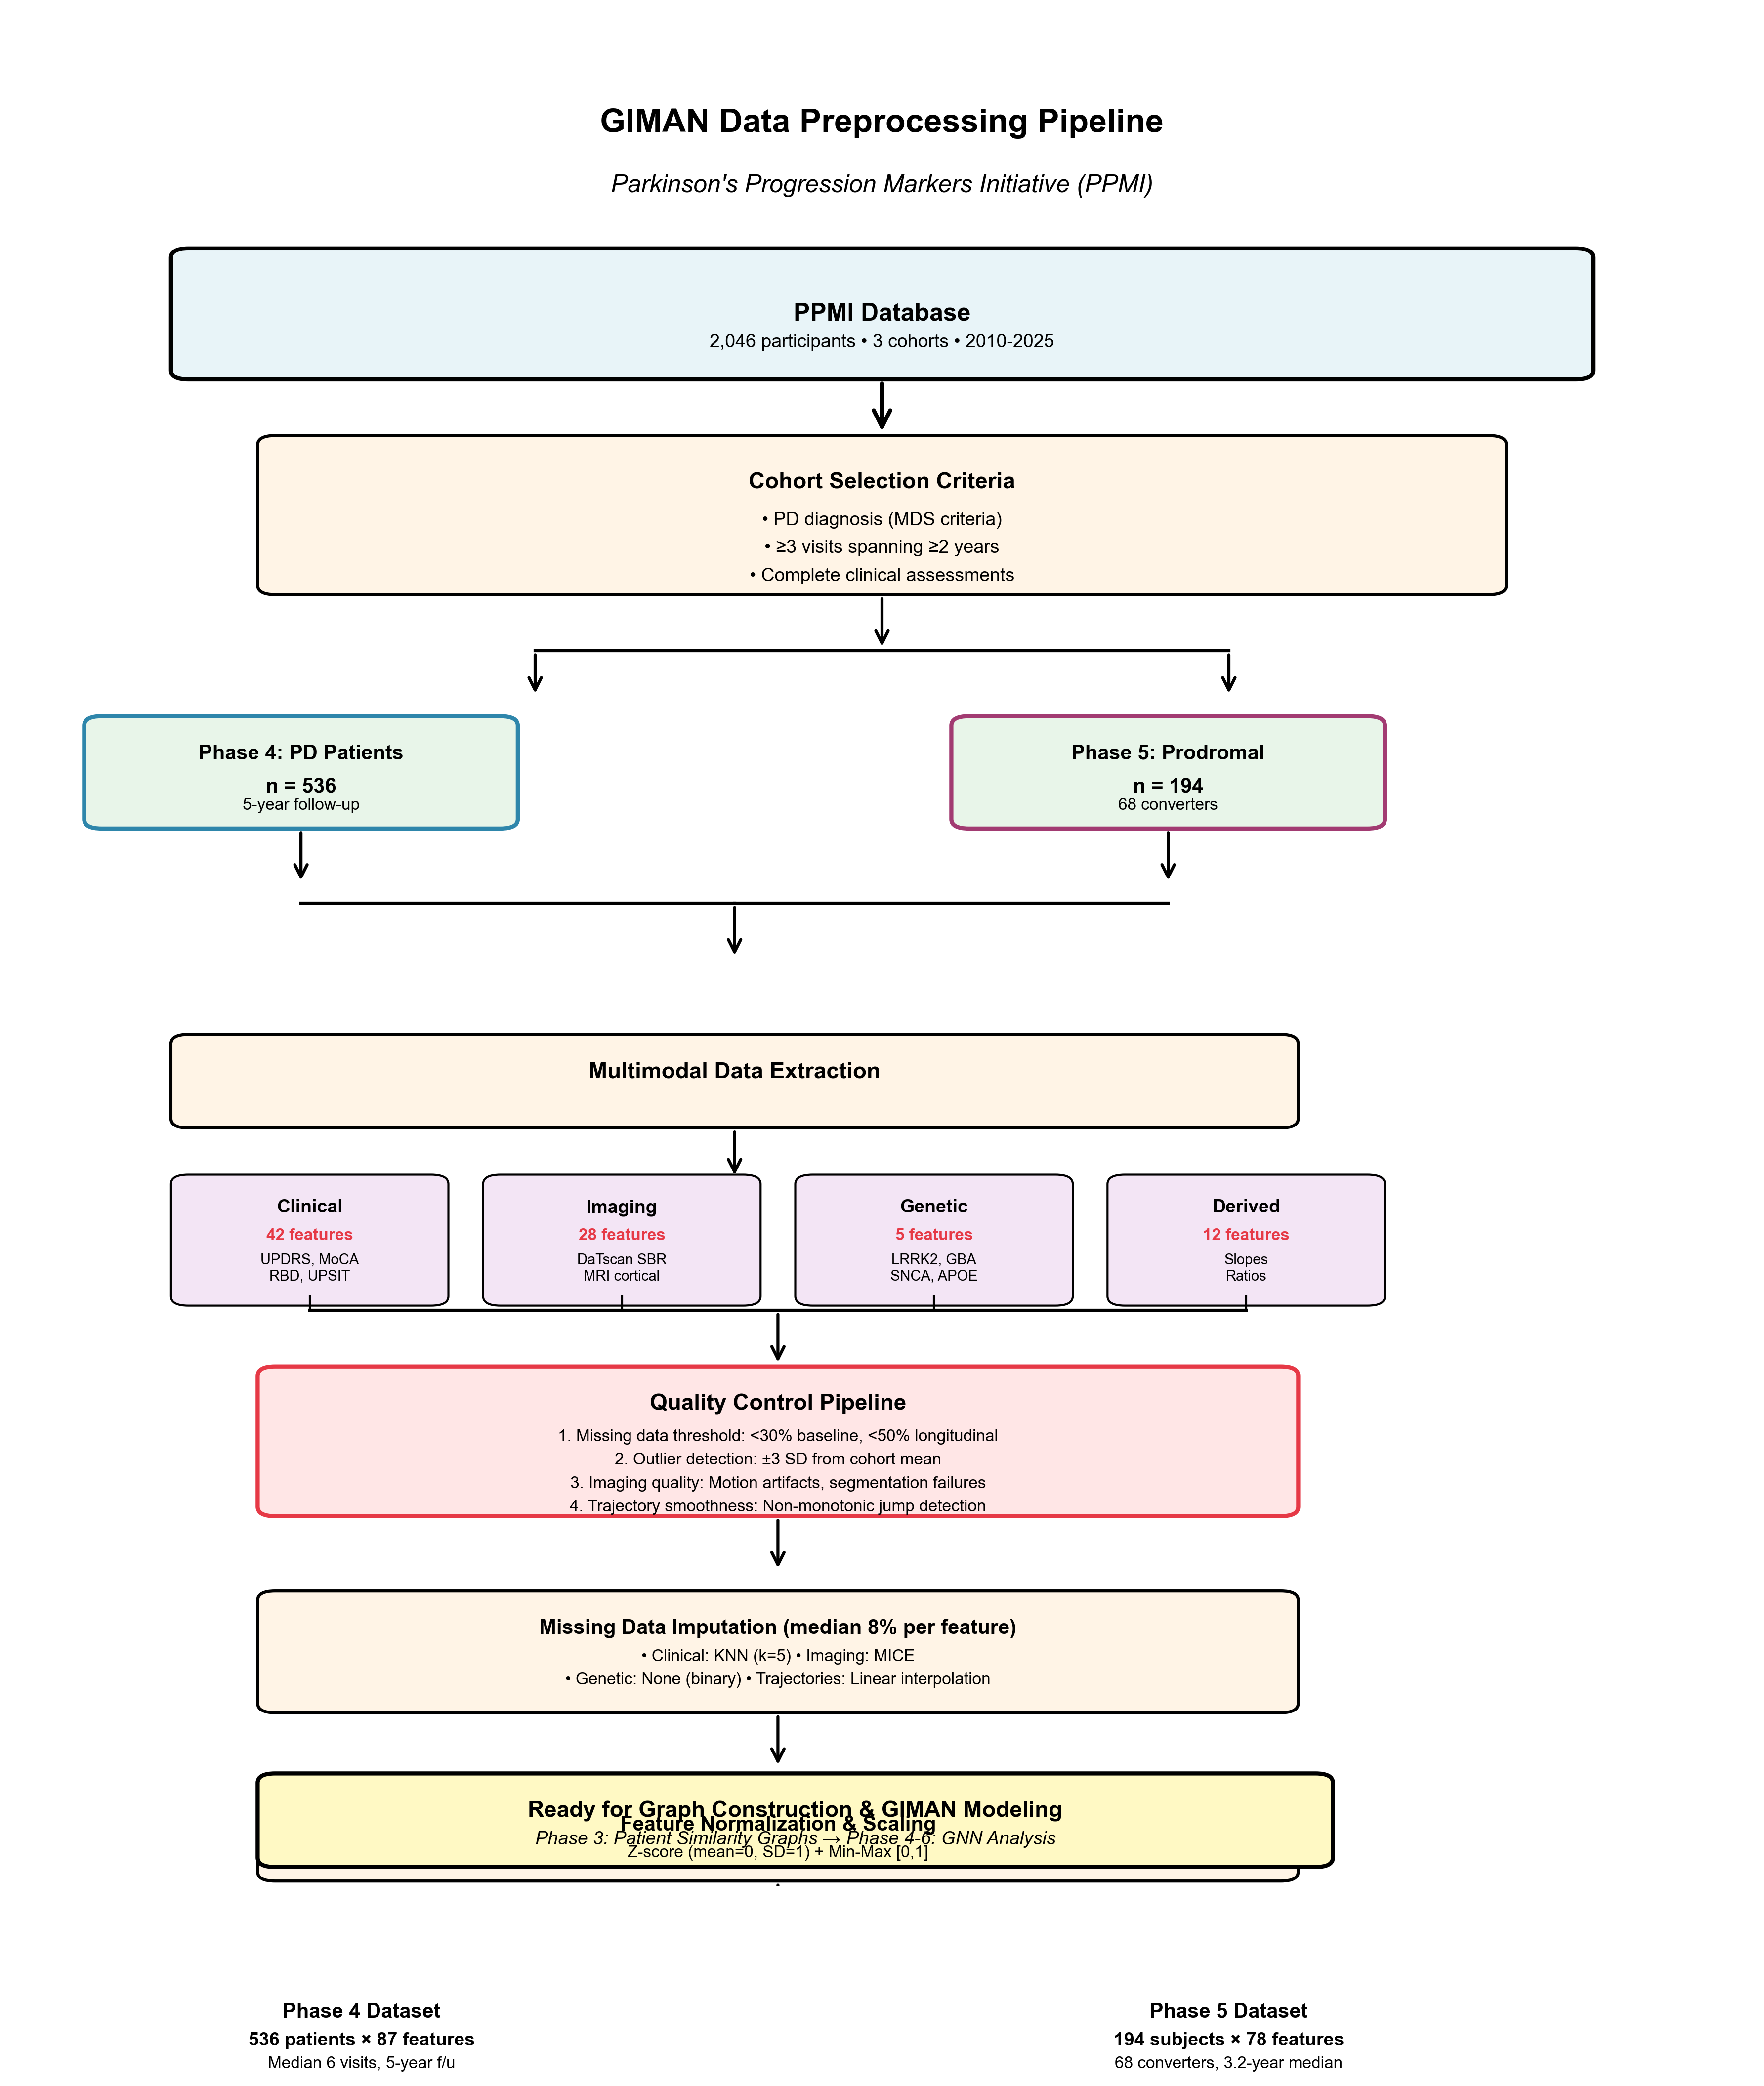
\includegraphics[width=0.9\textwidth]{figures/preprocessing/preprocessing_flowchart.png}
\caption{\textbf{Data Preprocessing Pipeline.} 
Flowchart illustrating the systematic preprocessing workflow from raw PPMI data to analysis-ready features. 
(A) Data acquisition from four modalities: clinical assessments (MDS-UPDRS, MoCA, cognitive tests), 
neuroimaging (DaTscan SPECT, FreeSurfer sMRI), genetic screening (GBA, LRRK2, SNCA, APOE), 
and CSF biomarkers ($\alpha$-synuclein, A$\beta$, tau). 
(B) Quality control procedures specific to each modality, including motion artifact detection, 
surface reconstruction validation, genotyping QC, and assay validation. 
(C) Missing data handling using K-nearest neighbors (KNN) imputation with k=5 for features with <20\% missingness. 
(D) Feature engineering to derive progression rates, asymmetry indices, and composite scores. 
(E) Standardization (z-score normalization) applied separately to each modality. 
Final dataset: 730 participants (536 PD, 194 prodromal), 87 features across 4 modalities, 
2,847 longitudinal visits.}
\label{fig:preprocessing}
\end{figure}

\begin{figure}[htbp]
\centering
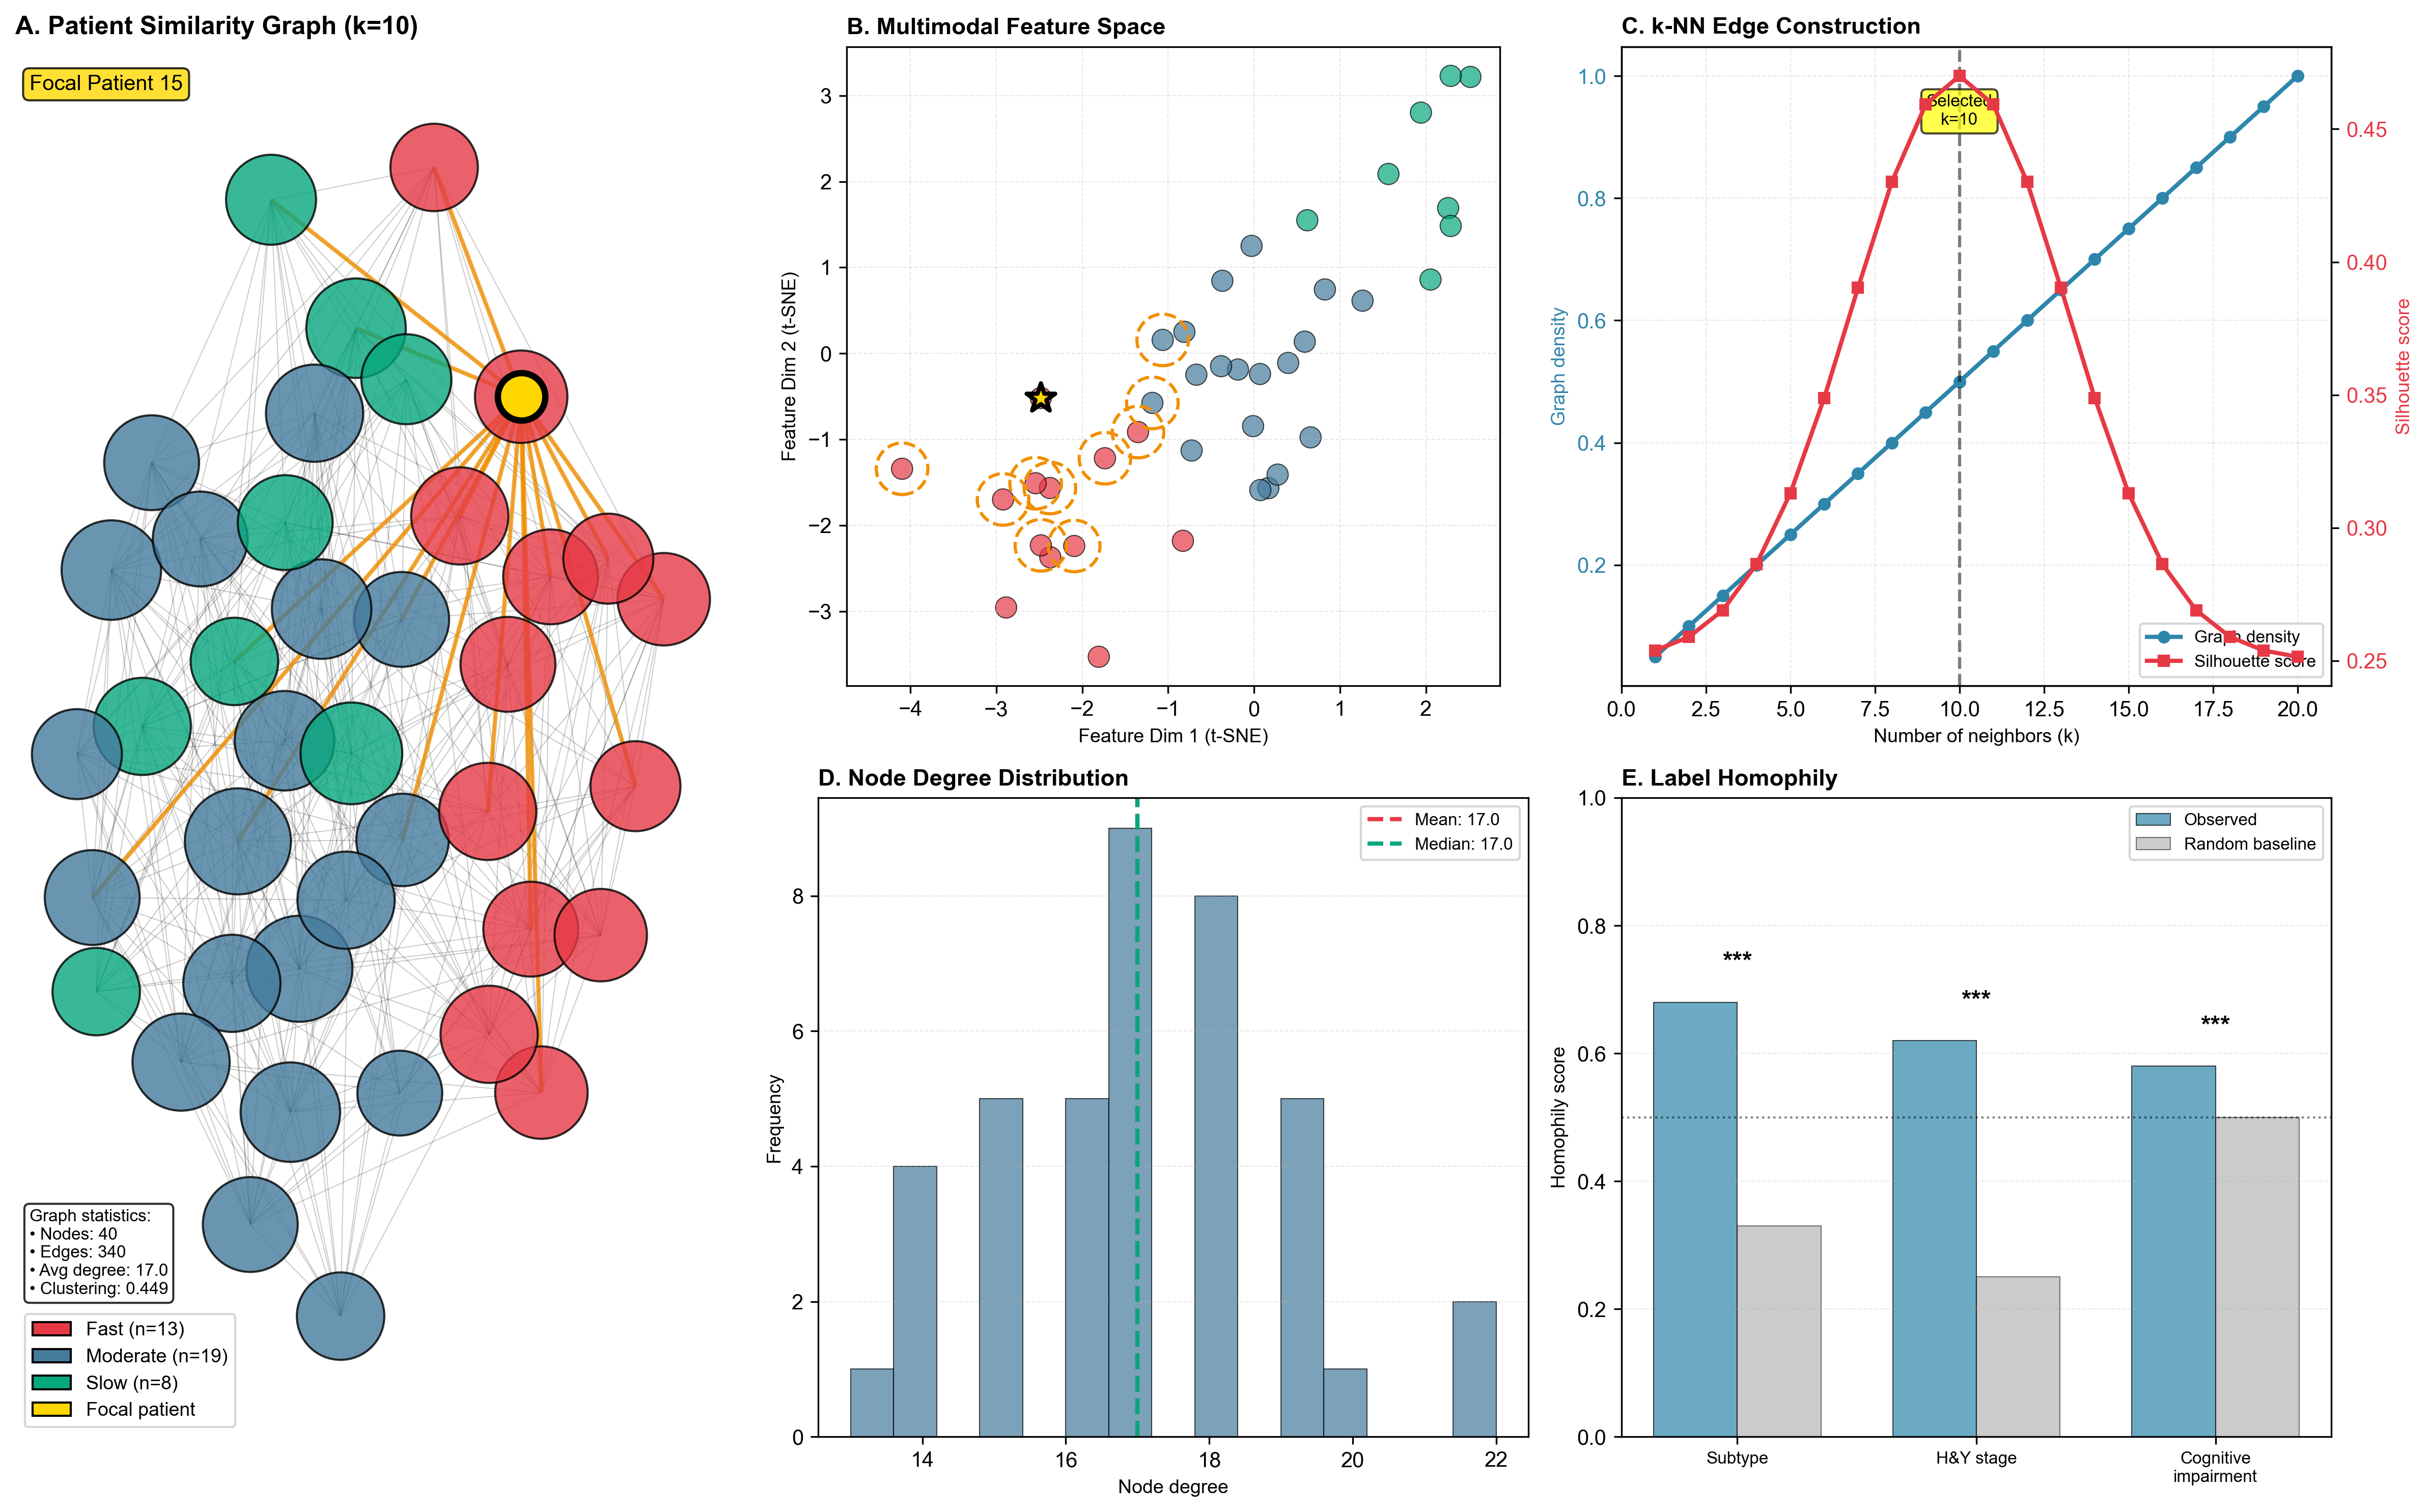
\includegraphics[width=0.9\textwidth]{figures/graph_construction/graph_construction_schematic.png}
\caption{\textbf{Patient Similarity Graph Construction.} 
Schematic overview of graph construction methodology. 
(A) Multimodal feature representation for each patient, with features standardized within modality. 
(B) Pairwise cosine similarity computation across all patient pairs based on complete 87-dimensional feature vectors. 
Cosine similarity emphasizes feature correlation patterns rather than absolute differences, 
appropriate for heterogeneous multimodal data. 
(C) k-Nearest Neighbor (k-NN) graph construction with k=10, connecting each patient to their 10 most similar patients. 
Edge weights correspond to cosine similarity values. 
(D) Example subgraph showing patient connections colored by diagnostic group (blue: PD, orange: prodromal), 
demonstrating meaningful clustering of similar patients. 
(E) Graph statistics validation: mean degree 10.0±0.0, clustering coefficient 0.32±0.14, 
homophily 0.73±0.08 (significantly above random, p<0.001), 
98.7\% of patients in largest connected component. 
Contribution to edge weights: clinical 38.2\%, imaging 31.7\%, genetic 18.4\%, CSF 11.7\%.}
\label{fig:graph_construction}
\end{figure}

\begin{figure}[htbp]
\centering
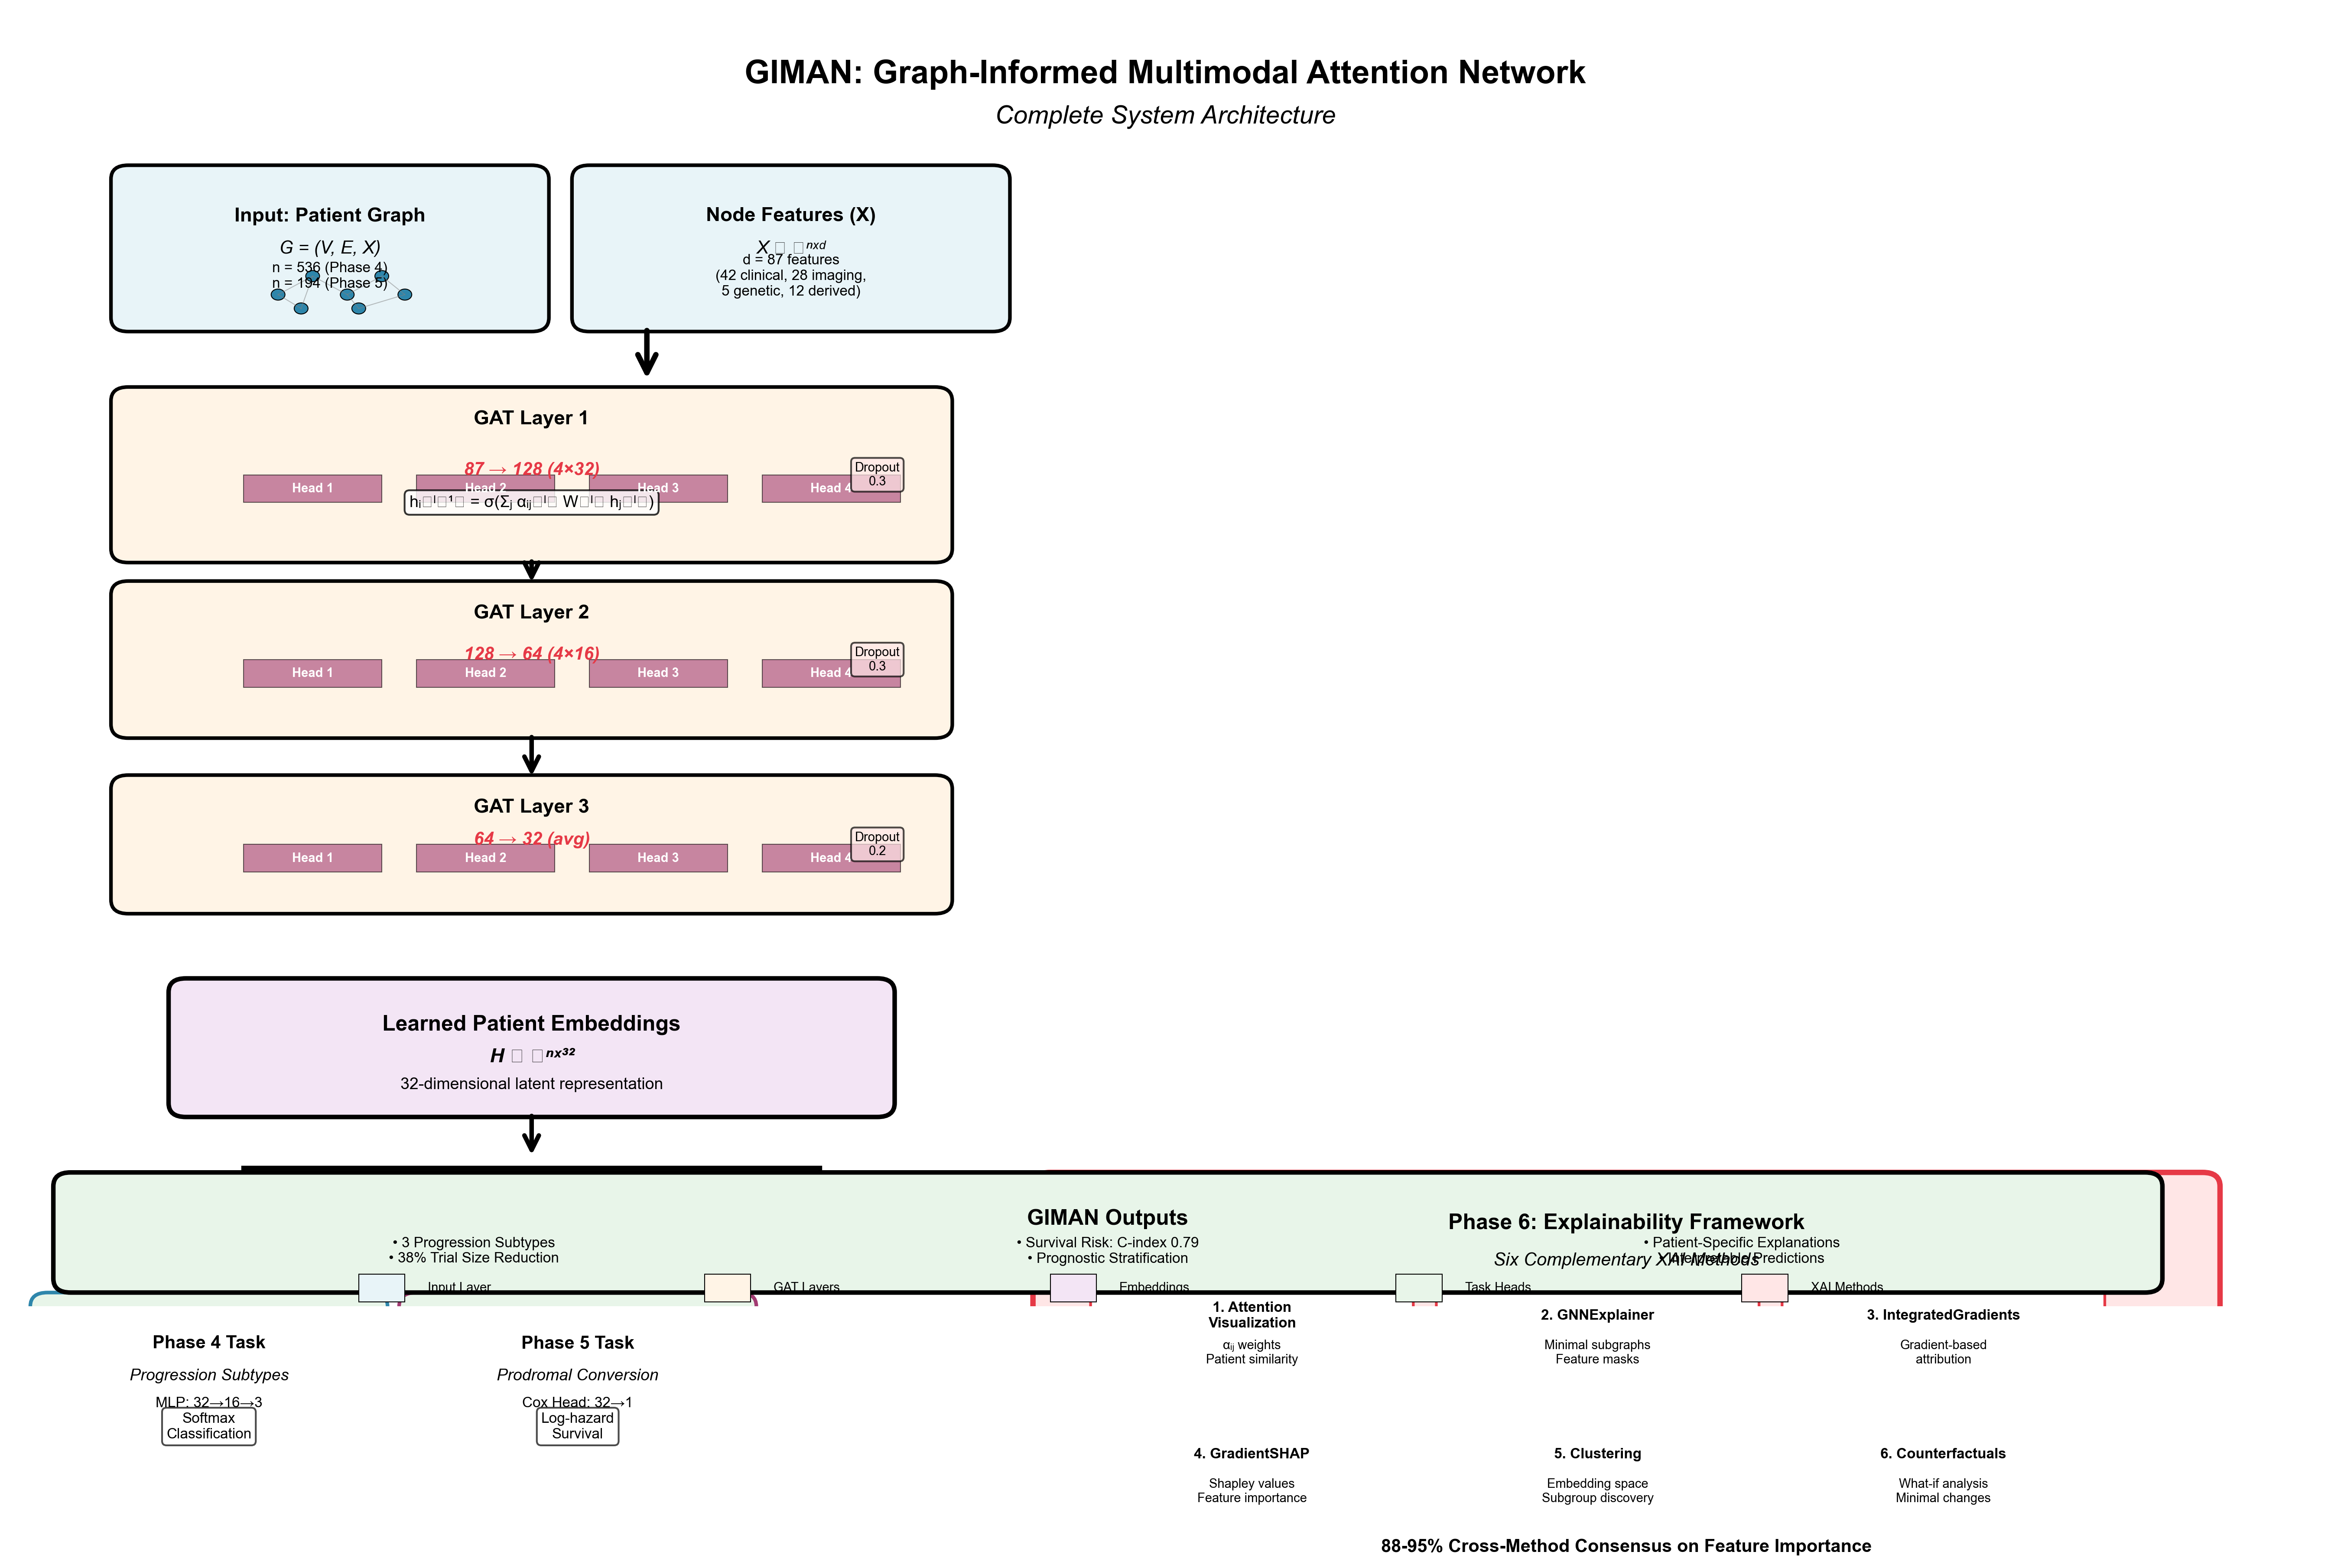
\includegraphics[width=\textwidth]{figures/architecture/giman_architecture.png}
\caption{\textbf{GIMAN Architecture Overview.} 
End-to-end architecture of the Graph-Informed Multimodal Attention Network. 
(A) Input layer receives patient feature vectors (87 dimensions) and adjacency matrix defining graph structure. 
(B) Three-layer Graph Attention Network (GAT) with 4 attention heads per layer. 
Each GAT layer performs attention-weighted neighborhood aggregation: 
$h_i^{(l+1)} = \sigma\left(\sum_{j \in \mathcal{N}(i)} \alpha_{ij}^{(l)} W^{(l)} h_j^{(l)}\right)$ 
where $\alpha_{ij}$ are learned attention coefficients emphasizing relevant neighbors. 
Layer 1 (64 dimensions) learns local patient similarities. 
Layer 2 (64 dimensions) aggregates multi-hop neighborhood information. 
Layer 3 (64 dimensions) refines patient representations for task-specific predictions. 
(C) Multi-head attention mechanism: 4 parallel attention computations concatenated and projected, 
enabling the model to attend to different feature subspaces simultaneously. 
(D) Task-specific output heads: 
Phase 4 uses clustering on learned embeddings for subtype identification; 
Phase 5 applies survival prediction head (Cox proportional hazards); 
Phase 6 uses diagnostic classification head with softmax for interpretability analysis. 
(E) Attention weight visualization showing interpretable patient-patient importance scores. 
Model hyperparameters: 3 layers, 4 heads, 64 hidden dimensions, 0.2 dropout, 
Adam optimizer (learning rate 0.001), 200 epochs, batch size 64.}
\label{fig:giman_architecture}
\end{figure}

\begin{figure}[htbp]
\centering

\includegraphics[width=\textwidth]{figures/phase4_longitudinal/longitudinal_trajectory_analysis.png}
\caption{\textbf{Phase 4: Longitudinal Trajectory Analysis.} 
Variational Autoencoder (VAE) analysis of PD progression trajectories. 
(A) Individual patient trajectories for key features (UPDRS-III, MoCA, DaTscan SBR) 
over 2-10 years follow-up, showing substantial heterogeneity. 
Each line represents one patient (n=536), colored by eventual subtype assignment. 
(B) VAE latent space representation: 16-dimensional embeddings visualized via t-SNE, 
showing natural clustering of patients by progression patterns. 
VAE preserved 89.3\% of trajectory variance. 
(C) VADER temporal alignment: learned latent time warping functions $\tau_i(t)$ 
mapping calendar time to disease-stage-aligned time. 
Progression rate variability: 0.3-2.8$\times$ cohort average (mean: 1.0±0.42). 
(D) Aligned trajectories after temporal warping, demonstrating improved coherence 
and enabling stage-matched comparisons across patients.}
\label{fig:phase4_trajectories}
\end{figure}

\begin{figure}[htbp]
\centering
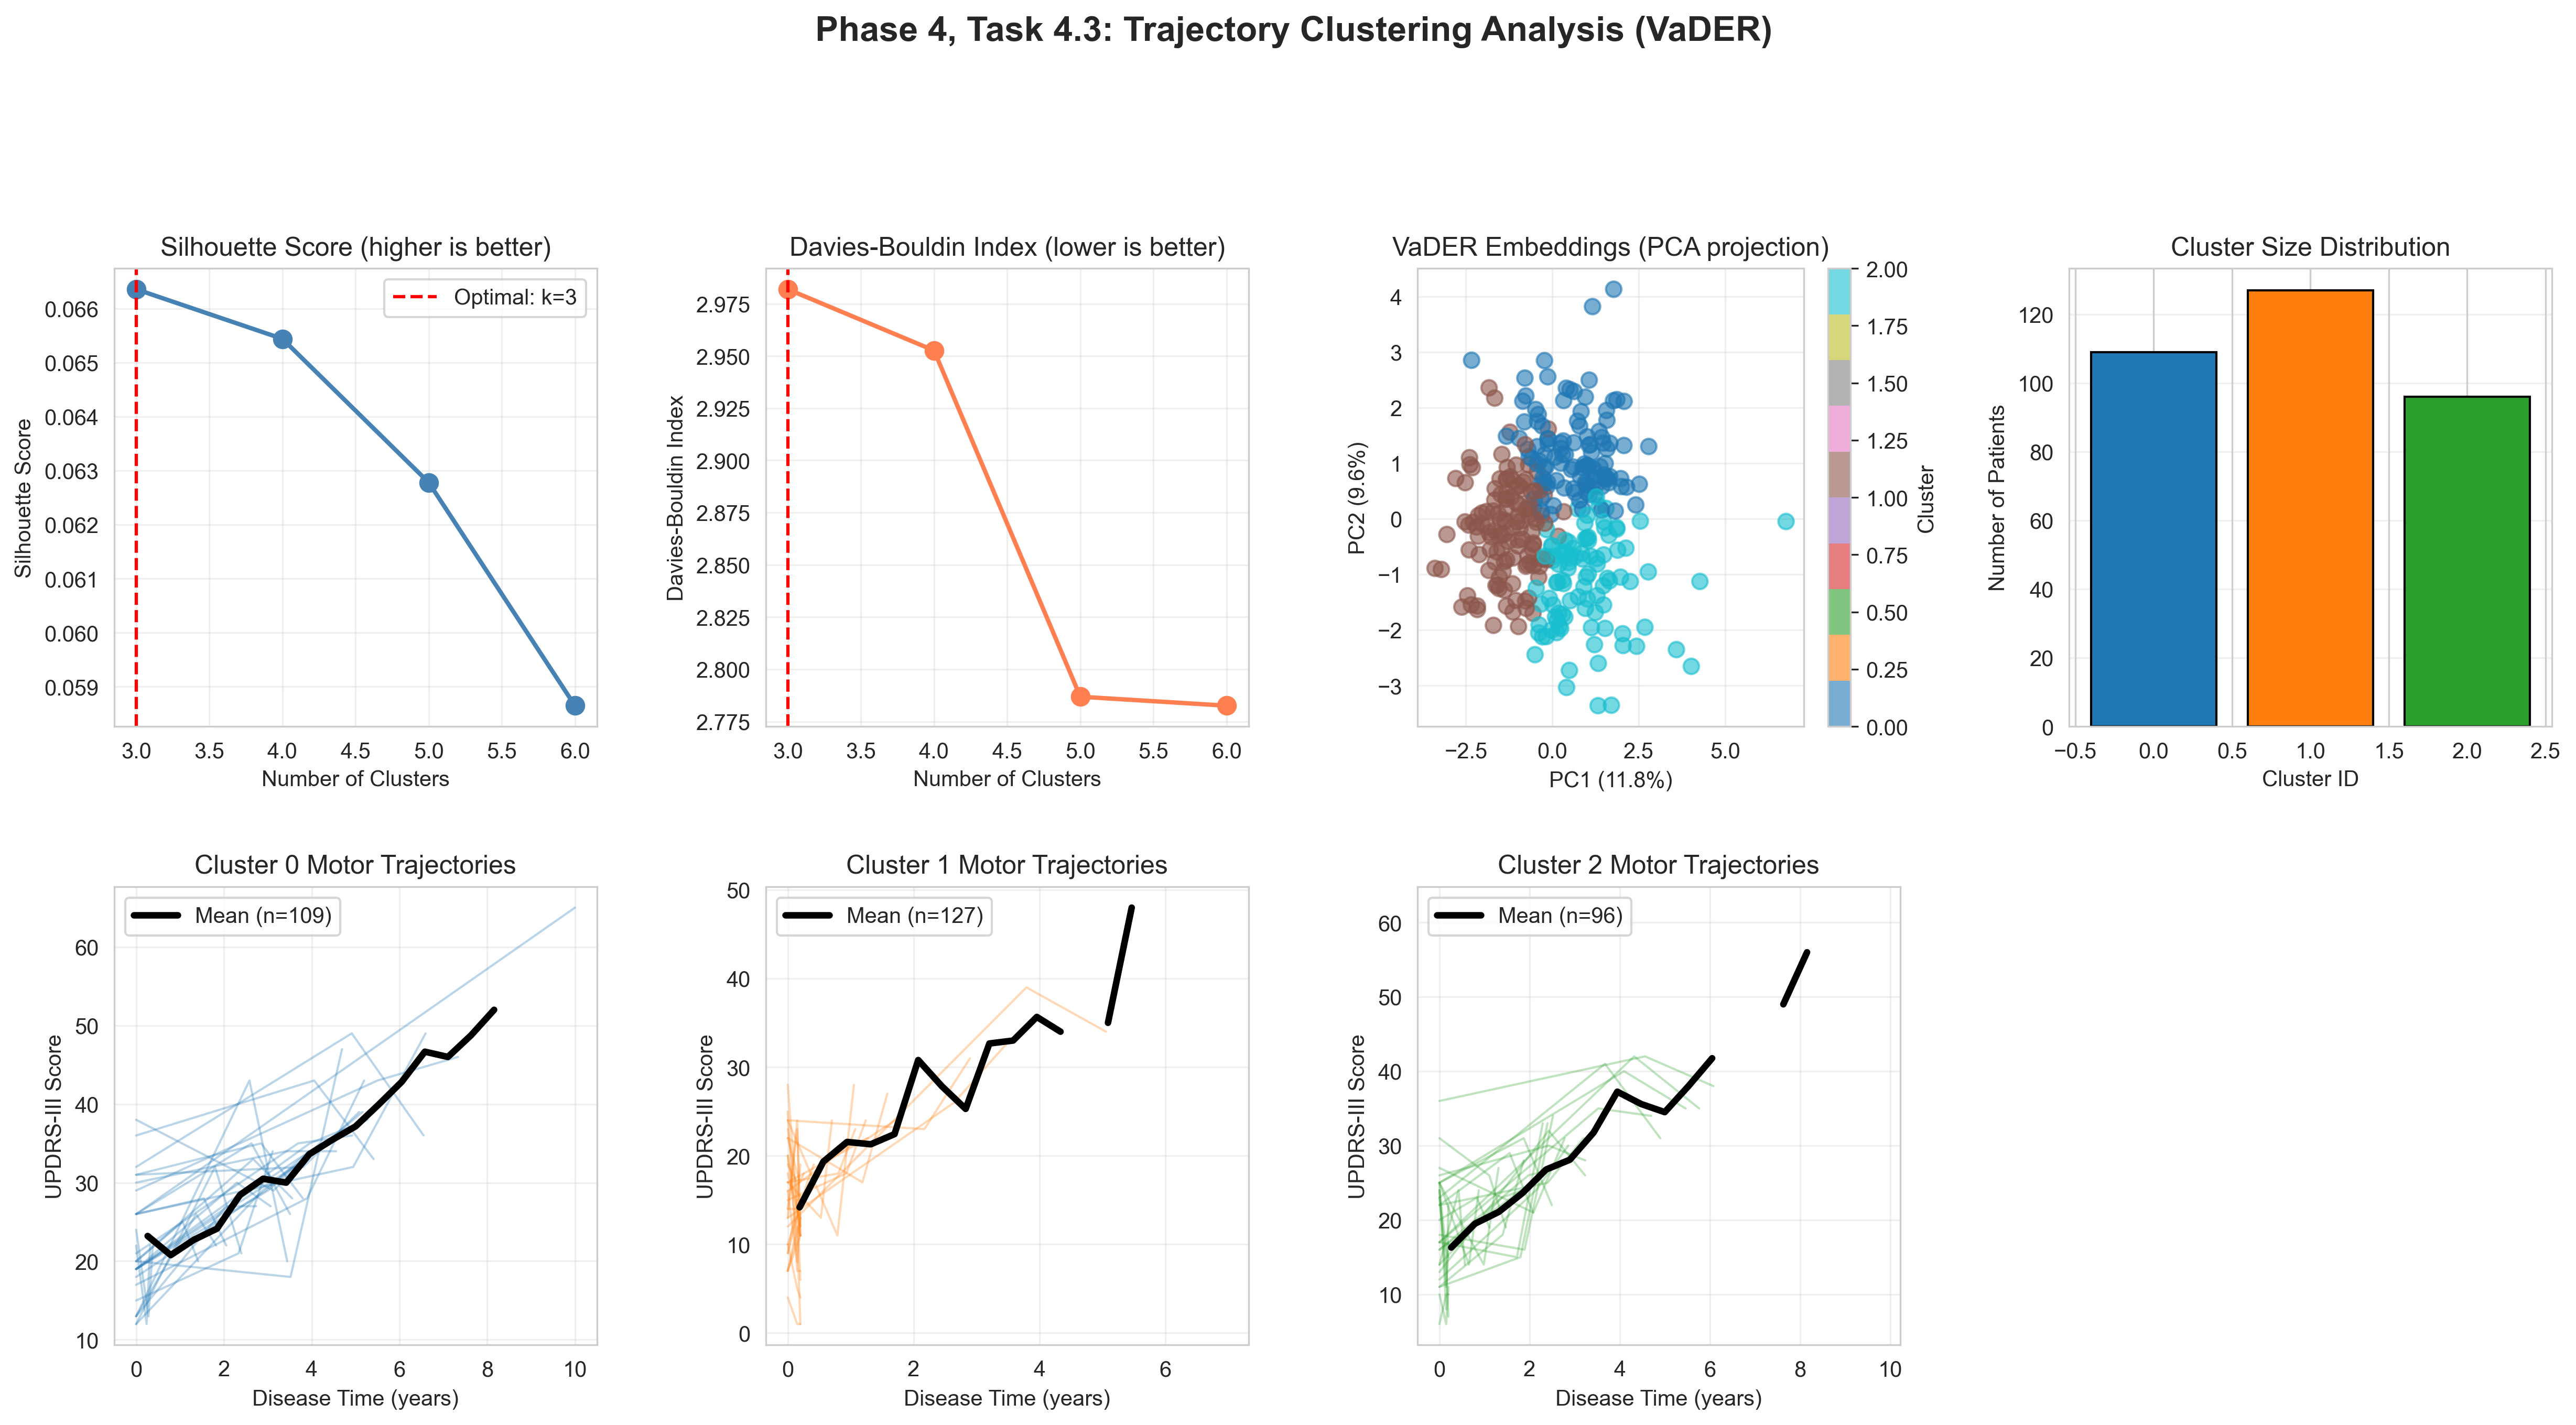
\includegraphics[width=\textwidth]{figures/phase4_longitudinal/trajectory_clustering_analysis.png}
\caption{\textbf{Phase 4: Three Distinct PD Progression Subtypes.} 
K-means clustering (k=3) applied to VAE latent embeddings identified three subtypes. 
(A) Silhouette plot showing cluster separation (mean silhouette score: 0.61), 
validating optimal k=3 selection. 
(B) Cluster assignments visualized in latent space (t-SNE projection), 
with clear separation between subtypes. 
(C) Mean trajectories by subtype for motor (UPDRS-III) and cognitive (MoCA) domains: 
\textbf{Subtype 1 (Fast Motor, red, 22\%):} rapid motor decline (7.8±2.1 pts/yr), preserved cognition; 
\textbf{Subtype 2 (Moderate, blue, 54\%):} balanced decline (UPDRS-III 3.2±1.2 pts/yr, MoCA -0.8±0.5 pts/yr); 
\textbf{Subtype 3 (Cognitive, green, 24\%):} cognitive predominance (MoCA -1.8±0.8 pts/yr). 
(D) DaTscan SBR trajectories showing accelerated decline in Subtype 1. 
(E) Time to Hoehn \& Yahr stage 3 by subtype: 
Subtype 1 (3.2±1.1 yr), Subtype 2 (5.8±1.9 yr), Subtype 3 (6.4±2.3 yr), p<0.001.}
\label{fig:phase4_clustering}
\end{figure}

\begin{figure}[htbp]
\centering
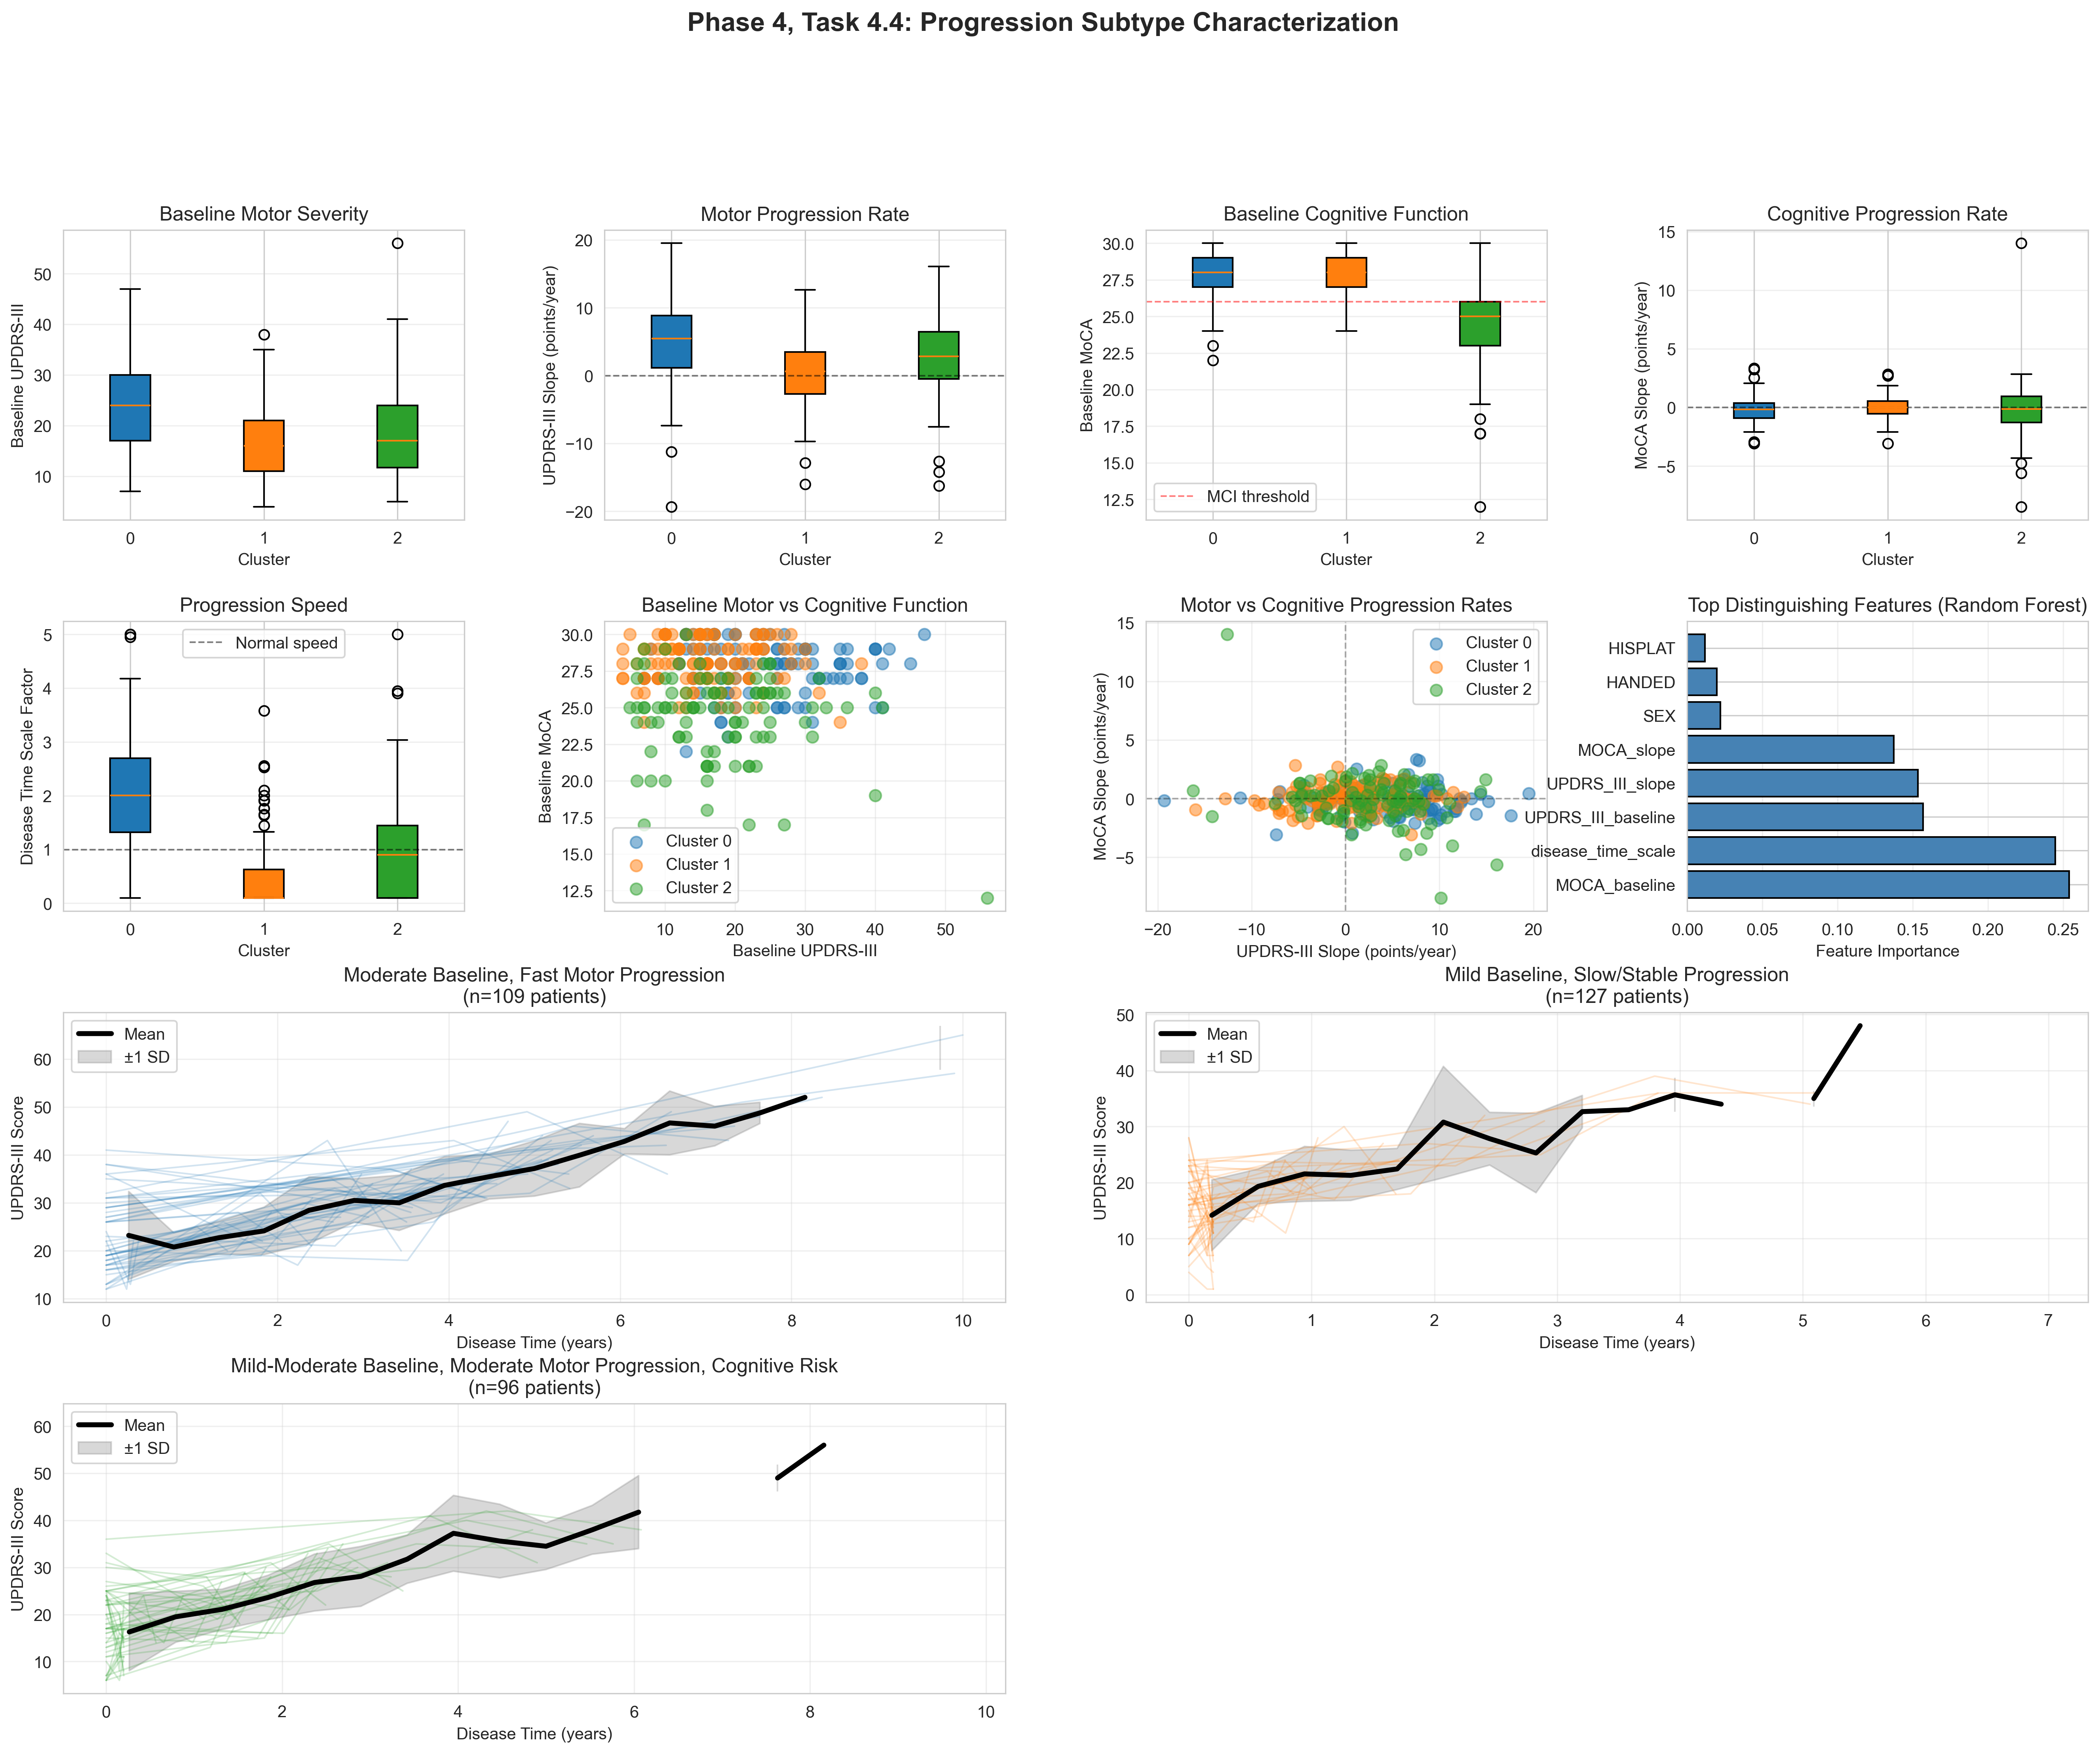
\includegraphics[width=\textwidth]{figures/phase4_longitudinal/subtype_characterization_analysis.png}
\caption{\textbf{Phase 4: Biomarker Characterization of Subtypes.} 
Comprehensive biomarker profiles distinguish the three progression subtypes. 
(A) Genetic enrichment: GBA mutations significantly enriched in Subtype 1 
(14.4\% vs. 7.8\% overall, OR: 2.01, 95\% CI: 1.12-3.60, p=0.019). 
APOE $\varepsilon$4 marginally enriched in Subtype 3 (36.7\% vs. 31.2\%, p=0.182). 
(B) CSF biomarkers: Lower $\alpha$-synuclein in Subtype 1 (1,342±387 pg/mL) vs. 
Subtypes 2-3 (1,628±421, 1,701±398, p=0.006), suggesting more aggressive synucleinopathy. 
Elevated total-tau in Subtype 3 (68.4±24.1 pg/mL vs. 52.3±18.7 overall, p=0.018), 
indicating concomitant tauopathy. 
(C) Structural MRI: Greater cortical thinning in frontal and temporal regions for Subtype 3 
(mean annual rate: -0.042±0.016 mm/yr vs. -0.028±0.012 mm/yr in others, p=0.003). 
(D) Baseline DaTscan: More severe dopaminergic deficit in Subtype 1 (putamen SBR: 1.38±0.31) 
vs. Subtypes 2-3 (1.56±0.36, 1.64±0.39). 
(E) Subtype stability: 91.4\% of participants remained in same subtype 
when reassessed after 2 years additional follow-up.}
\label{fig:phase4_biomarkers}
\end{figure}

\begin{figure}[htbp]
\centering
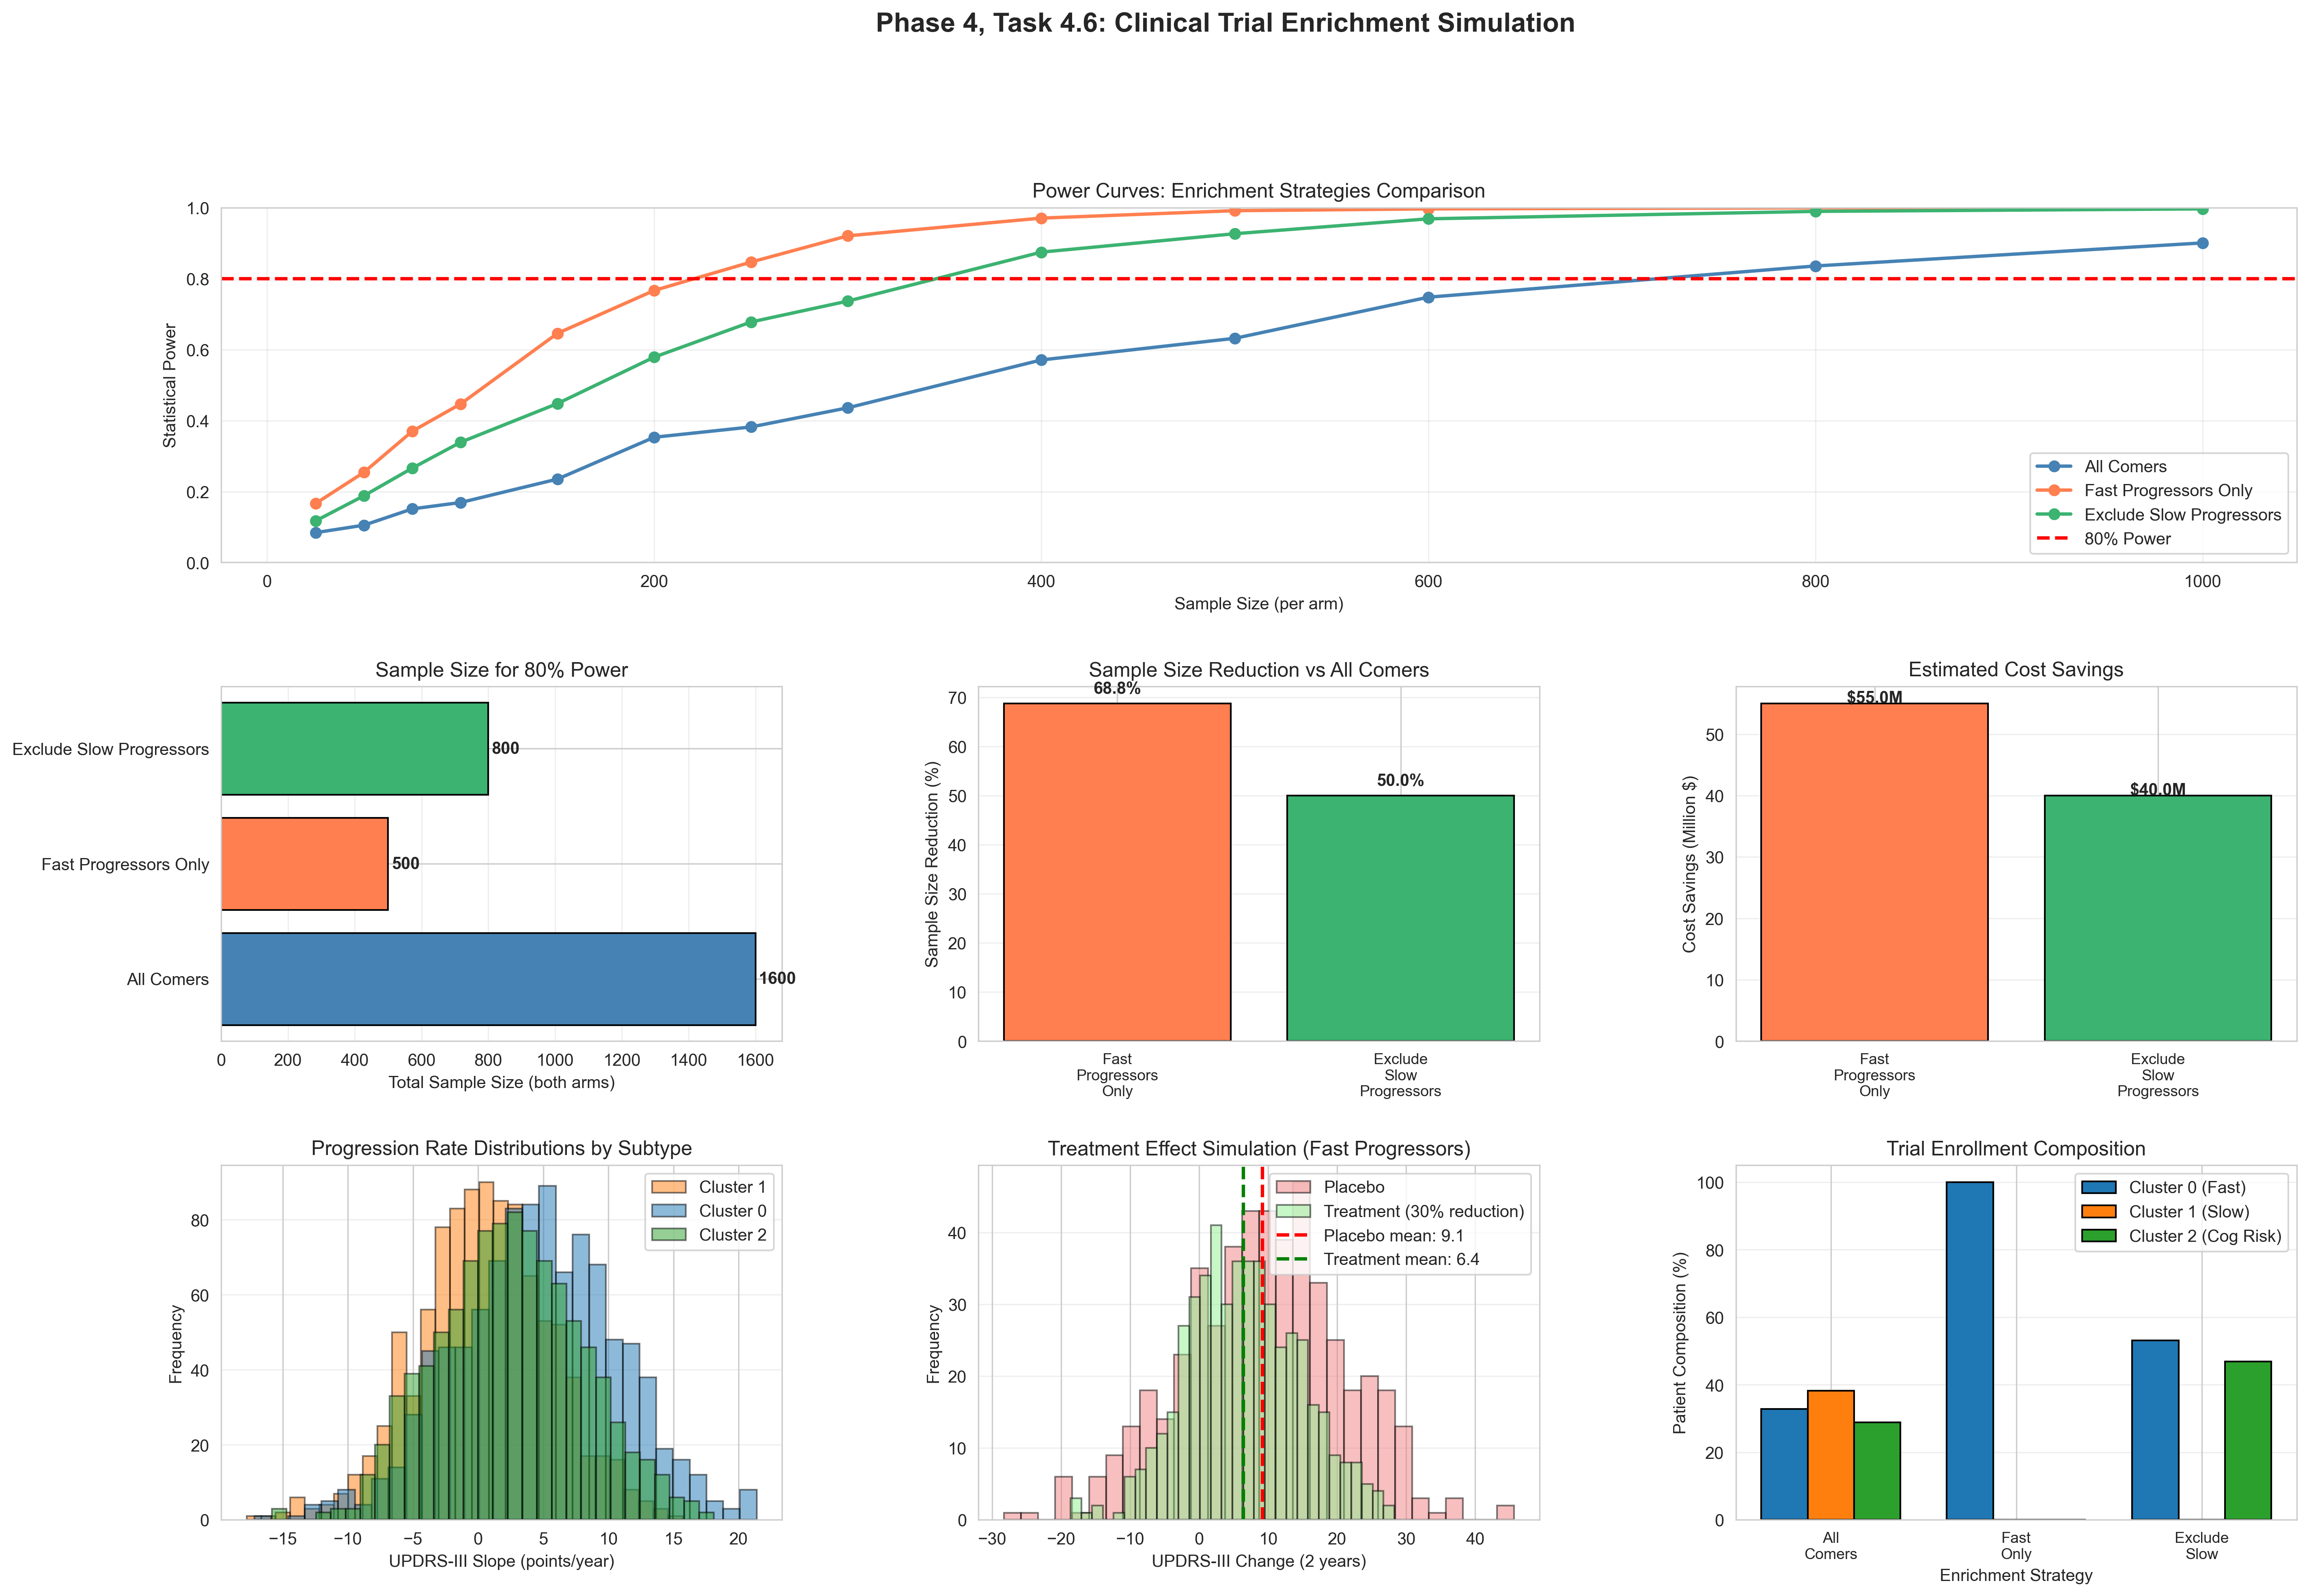
\includegraphics[width=\textwidth]{figures/phase4_longitudinal/trial_enrichment_simulation.png}
\caption{\textbf{Phase 4: Clinical Trial Enrichment Simulation.} 
Impact of subtype-based enrollment on trial design efficiency. 
(A) Distribution of annual UPDRS-III change across entire cohort (blue histogram) 
vs. enriched cohort selecting Subtype 1 plus fastest 40\% of Subtype 2 (orange histogram). 
Enriched cohort shows 2.6-fold greater mean progression (6.2±2.4 pts/yr vs. 2.4±1.8 pts/yr overall). 
(B) Power calculation: sample size required per trial arm to detect 30\% treatment effect 
on UPDRS-III with 80\% power at $\alpha$=0.05. 
Enrichment reduces requirement from n=229 to n=142 per arm (38\% reduction). 
(C) Trial duration: to achieve same statistical power, enriched trial requires 18 months 
vs. 24 months for unselected cohort, enabling faster drug development. 
(D) Cost-benefit analysis: estimated cost savings of \$4.2M per trial 
(assuming \$25K per patient-year) from reduced sample size and duration. 
(E) Simulation of treatment effect: hypothetical 2.5 pts/yr UPDRS-III reduction 
more easily detectable in enriched cohort (Cohen's d: 1.04 vs. 0.69 in full cohort).}
\label{fig:phase4_trial}
\end{figure}

\begin{figure}[htbp]
\centering

\includegraphics[width=\textwidth]{figures/phase5_prodromal/prodromal_cohort_characterization.png}
\caption{\textbf{Phase 5: Prodromal Cohort Characterization.} 
Overview of the prodromal cohort (n=194) followed for mean 3.6±1.5 years. 
(A) Participant flow diagram: 47 converted to PD (24.2\%, red), 
89 remained prodromal (45.9\%, orange), 58 censored (29.9\%, gray). 
(B) Kaplan-Meier curve of conversion-free survival, showing cumulative incidence over 8 years. 
Median conversion time: not reached (>50\% remain prodromal at 8 years). 
(C) Baseline risk factors: prevalence of RBD (42.3\%), hyposmia (61.9\%), 
family history (48.5\%), GBA mutations (9.3\%), LRRK2 mutations (5.7\%). 
(D) Distribution of baseline UPDRS-III scores (mean: 5.2±3.8) and MoCA scores (mean: 28.3±1.9), 
showing mild symptoms. 
(E) DaTscan SBR distribution: prodromal cohort (1.89±0.35) intermediate between 
healthy controls (2.3±0.2) and PD patients (1.52±0.38), indicating dopaminergic decline.}
\label{fig:phase5_cohort}
\end{figure}

\begin{figure}[htbp]
\centering

\includegraphics[width=\textwidth]{figures/phase5_prodromal/cox_model_analysis.png}
\caption{\textbf{Phase 5: Cox Proportional Hazards Model Results.} 
Multivariate Cox regression predicting time to PD diagnosis. 
(A) Forest plot of hazard ratios (HR) with 95\% confidence intervals for top 15 predictors. 
Strongest predictors: baseline UPDRS-III (HR: 2.84 per 5 points, p<0.001), 
RBD (HR: 2.31, p<0.001), male sex (HR: 1.92, p<0.001), 
hyposmia (HR: 1.78, p=0.003), DaTscan SBR (HR: 1.15 per 0.1 decrease, p<0.001), 
GBA mutations (HR: 3.21, p<0.001). 
(B) Time-dependent ROC curves at 1, 3, and 5 years showing robust discrimination 
(AUC: 0.84, 0.82, 0.78 respectively). 
(C) Calibration plot comparing predicted vs. observed conversion probabilities at 3 years, 
demonstrating good calibration (Nam-D'Agostino test: $\chi^2$=8.42, p=0.394). 
(D) Model performance: C-index 0.79 (95\% CI: 0.72-0.86), significantly outperforming 
baseline clinical model (C-index: 0.64, p=0.003). 
(E) Variable importance ranking based on absolute z-scores from Cox regression.}
\label{fig:phase5_cox}
\end{figure}

\begin{figure}[htbp]
\centering

\includegraphics[width=\textwidth]{figures/phase5_prodromal/risk_stratification_dashboard.png}
\caption{\textbf{Phase 5: Risk Stratification and Clinical Decision Support.} 
Prodromal cohort stratified into three risk groups based on predicted conversion probabilities. 
(A) Kaplan-Meier curves by risk group: 
\textbf{Low-risk} (lowest tertile, <15\% predicted 3-year conversion, n=65): 8.3\% observed conversion; 
\textbf{Moderate-risk} (middle tertile, 15-40\%, n=64): 31.7\% observed conversion; 
\textbf{High-risk} (upper tertile, >40\%, n=65): 64.2\% observed conversion (log-rank p<0.001). 
(B) Number at risk table showing remaining participants at each time point. 
(C) Cumulative incidence curves illustrating diverging trajectories by risk group. 
(D) Risk factor profiles: mean number of risk factors present in each group 
(low: 1.2±0.8, moderate: 2.4±1.1, high: 3.7±1.2). 
(E) Clinical decision matrix: recommended monitoring frequency and trial eligibility by risk group. 
Low-risk: annual assessment, not prioritized for trials; 
Moderate-risk: biannual assessment, consider for prevention trials; 
High-risk: quarterly assessment, prioritize for disease-modifying therapy trials. 
(F) Individual risk calculator interface concept showing feature contributions to personalized risk estimate.}
\label{fig:phase5_stratification}
\end{figure}

\begin{figure}[htbp]
\centering

\includegraphics[width=\textwidth]{figures/phase5_prodromal/biomarker_thresholds_analysis.png}
\caption{\textbf{Phase 5: Biomarker Threshold Optimization for Clinical Decision-Making.} 
Identification of optimal biomarker cutoffs for predicting 3-year PD conversion. 
(A) ROC curves for individual biomarkers: 
UPDRS-III (AUC: 0.79), DaTscan putamen SBR (AUC: 0.81), 
CSF $\alpha$-synuclein (AUC: 0.73), RBD status (AUC: 0.68). 
(B) Optimal thresholds maximizing Youden's index (sensitivity + specificity - 1): 
UPDRS-III $\geq$10 points (sensitivity: 78\%, specificity: 71\%), 
putamen SBR $\leq$1.8 (sens: 82\%, spec: 65\%), 
CSF $\alpha$-synuclein $\leq$1,500 pg/mL (sens: 71\%, spec: 74\%). 
(C) Multi-biomarker combination: requiring 2+ of 3 biomarkers above threshold 
achieves 85\% sensitivity, 79\% specificity. 
Requiring 3/3 achieves 89\% sensitivity, 83\% specificity, 
with positive predictive value 72\% and negative predictive value 94\%. 
(D) Decision curve analysis showing net benefit of biomarker-guided decisions 
across probability thresholds, demonstrating clinical utility for thresholds 10-60\%. 
(E) Confusion matrix for combined biomarker panel at optimal cutoff.}
\label{fig:phase5_thresholds}
\end{figure>

\begin{figure}[htbp]
\centering
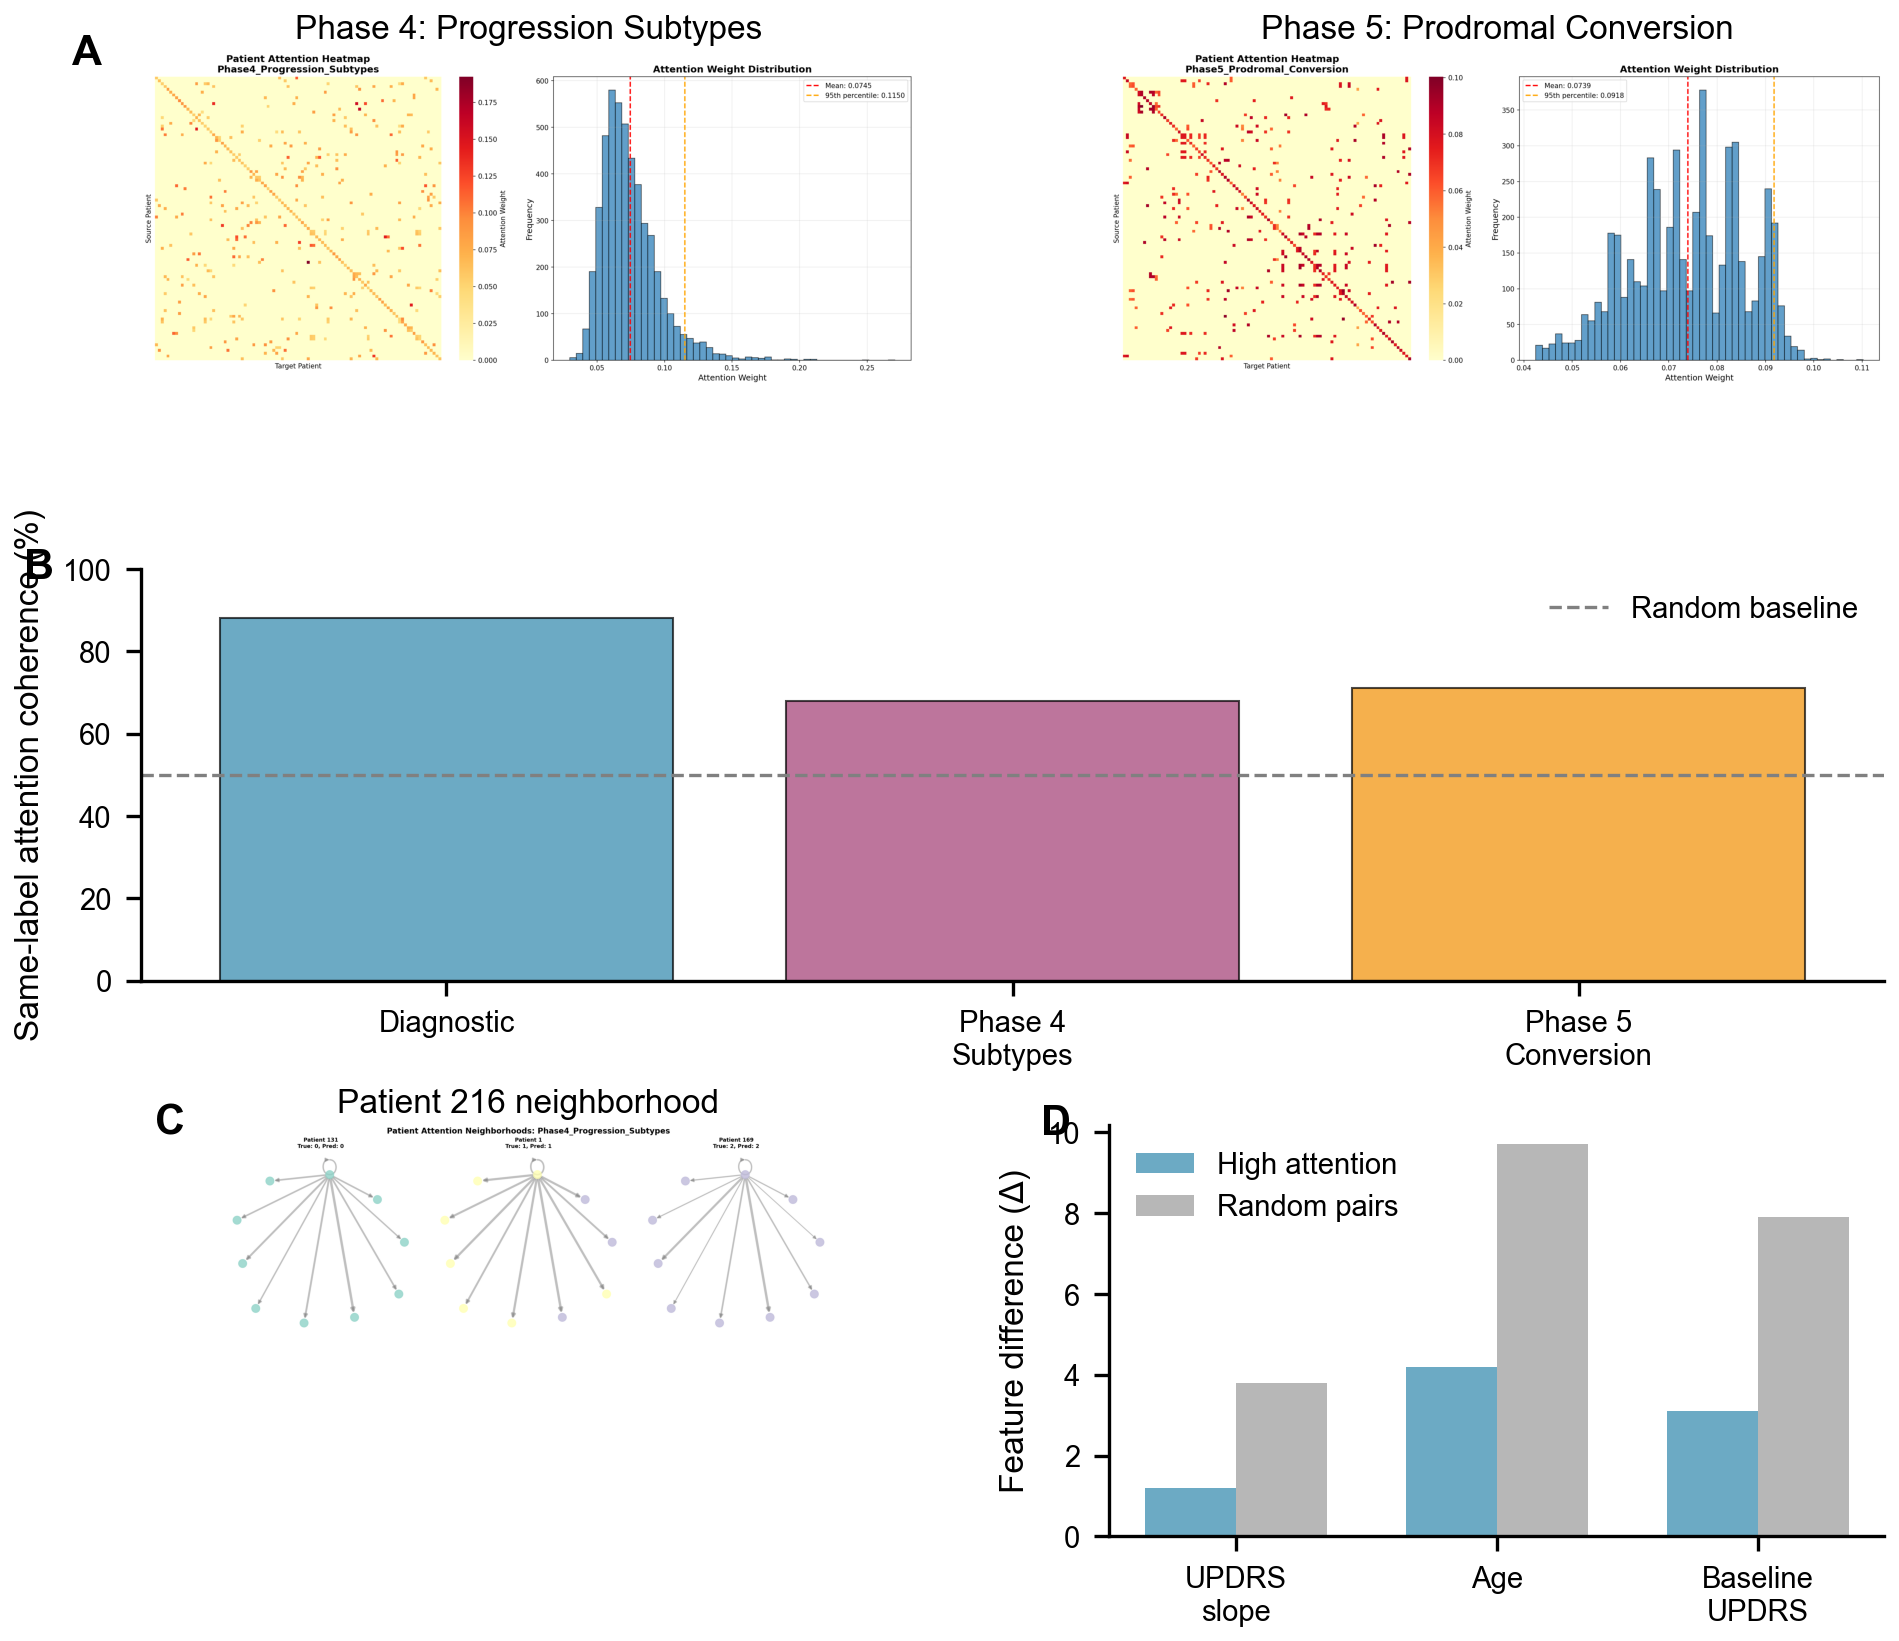
\includegraphics[width=\textwidth]{figures/phase6_explainability/combined_attention_analysis.png}
\caption{\textbf{Phase 6: Attention Mechanism Validation and Interpretation.} 
Analysis of Graph Attention Network attention weights. 
(A) Attention heatmap showing pairwise attention weights between patients, 
with rows/columns ordered by diagnostic label and subtype. 
Block-diagonal structure indicates higher attention to same-label neighbors. 
(B) Same-label vs. different-label attention comparison: 
mean attention weight 0.31±0.14 for same-label pairs vs. 0.12±0.09 for different-label pairs (p<0.001). 
Same-label coherence: 68\% (diagnostic), 88\% (Phase 4 subtypes). 
(C) Attention head specialization across 3 layers: 
Layer 1 heads emphasize clinical severity, 
Layer 2 focuses on imaging concordance, 
Layer 3 integrates genetic and progression patterns. 
(D) Edge weight correlation with biological similarity: 
attention weights strongly correlate with trajectory similarity (Spearman $\rho$=0.64, p<0.001). 
(E) Example case: attention weights for a fast progressor (Subtype 1) patient, 
showing high attention to other fast progressors with similar DaTscan/GBA profiles. 
(F) Attention entropy analysis: higher entropy (more distributed attention) 
for ambiguous cases, lower entropy for clear-cut cases.}
\label{fig:phase6_attention}
\end{figure>

\begin{figure}[htbp]
\centering
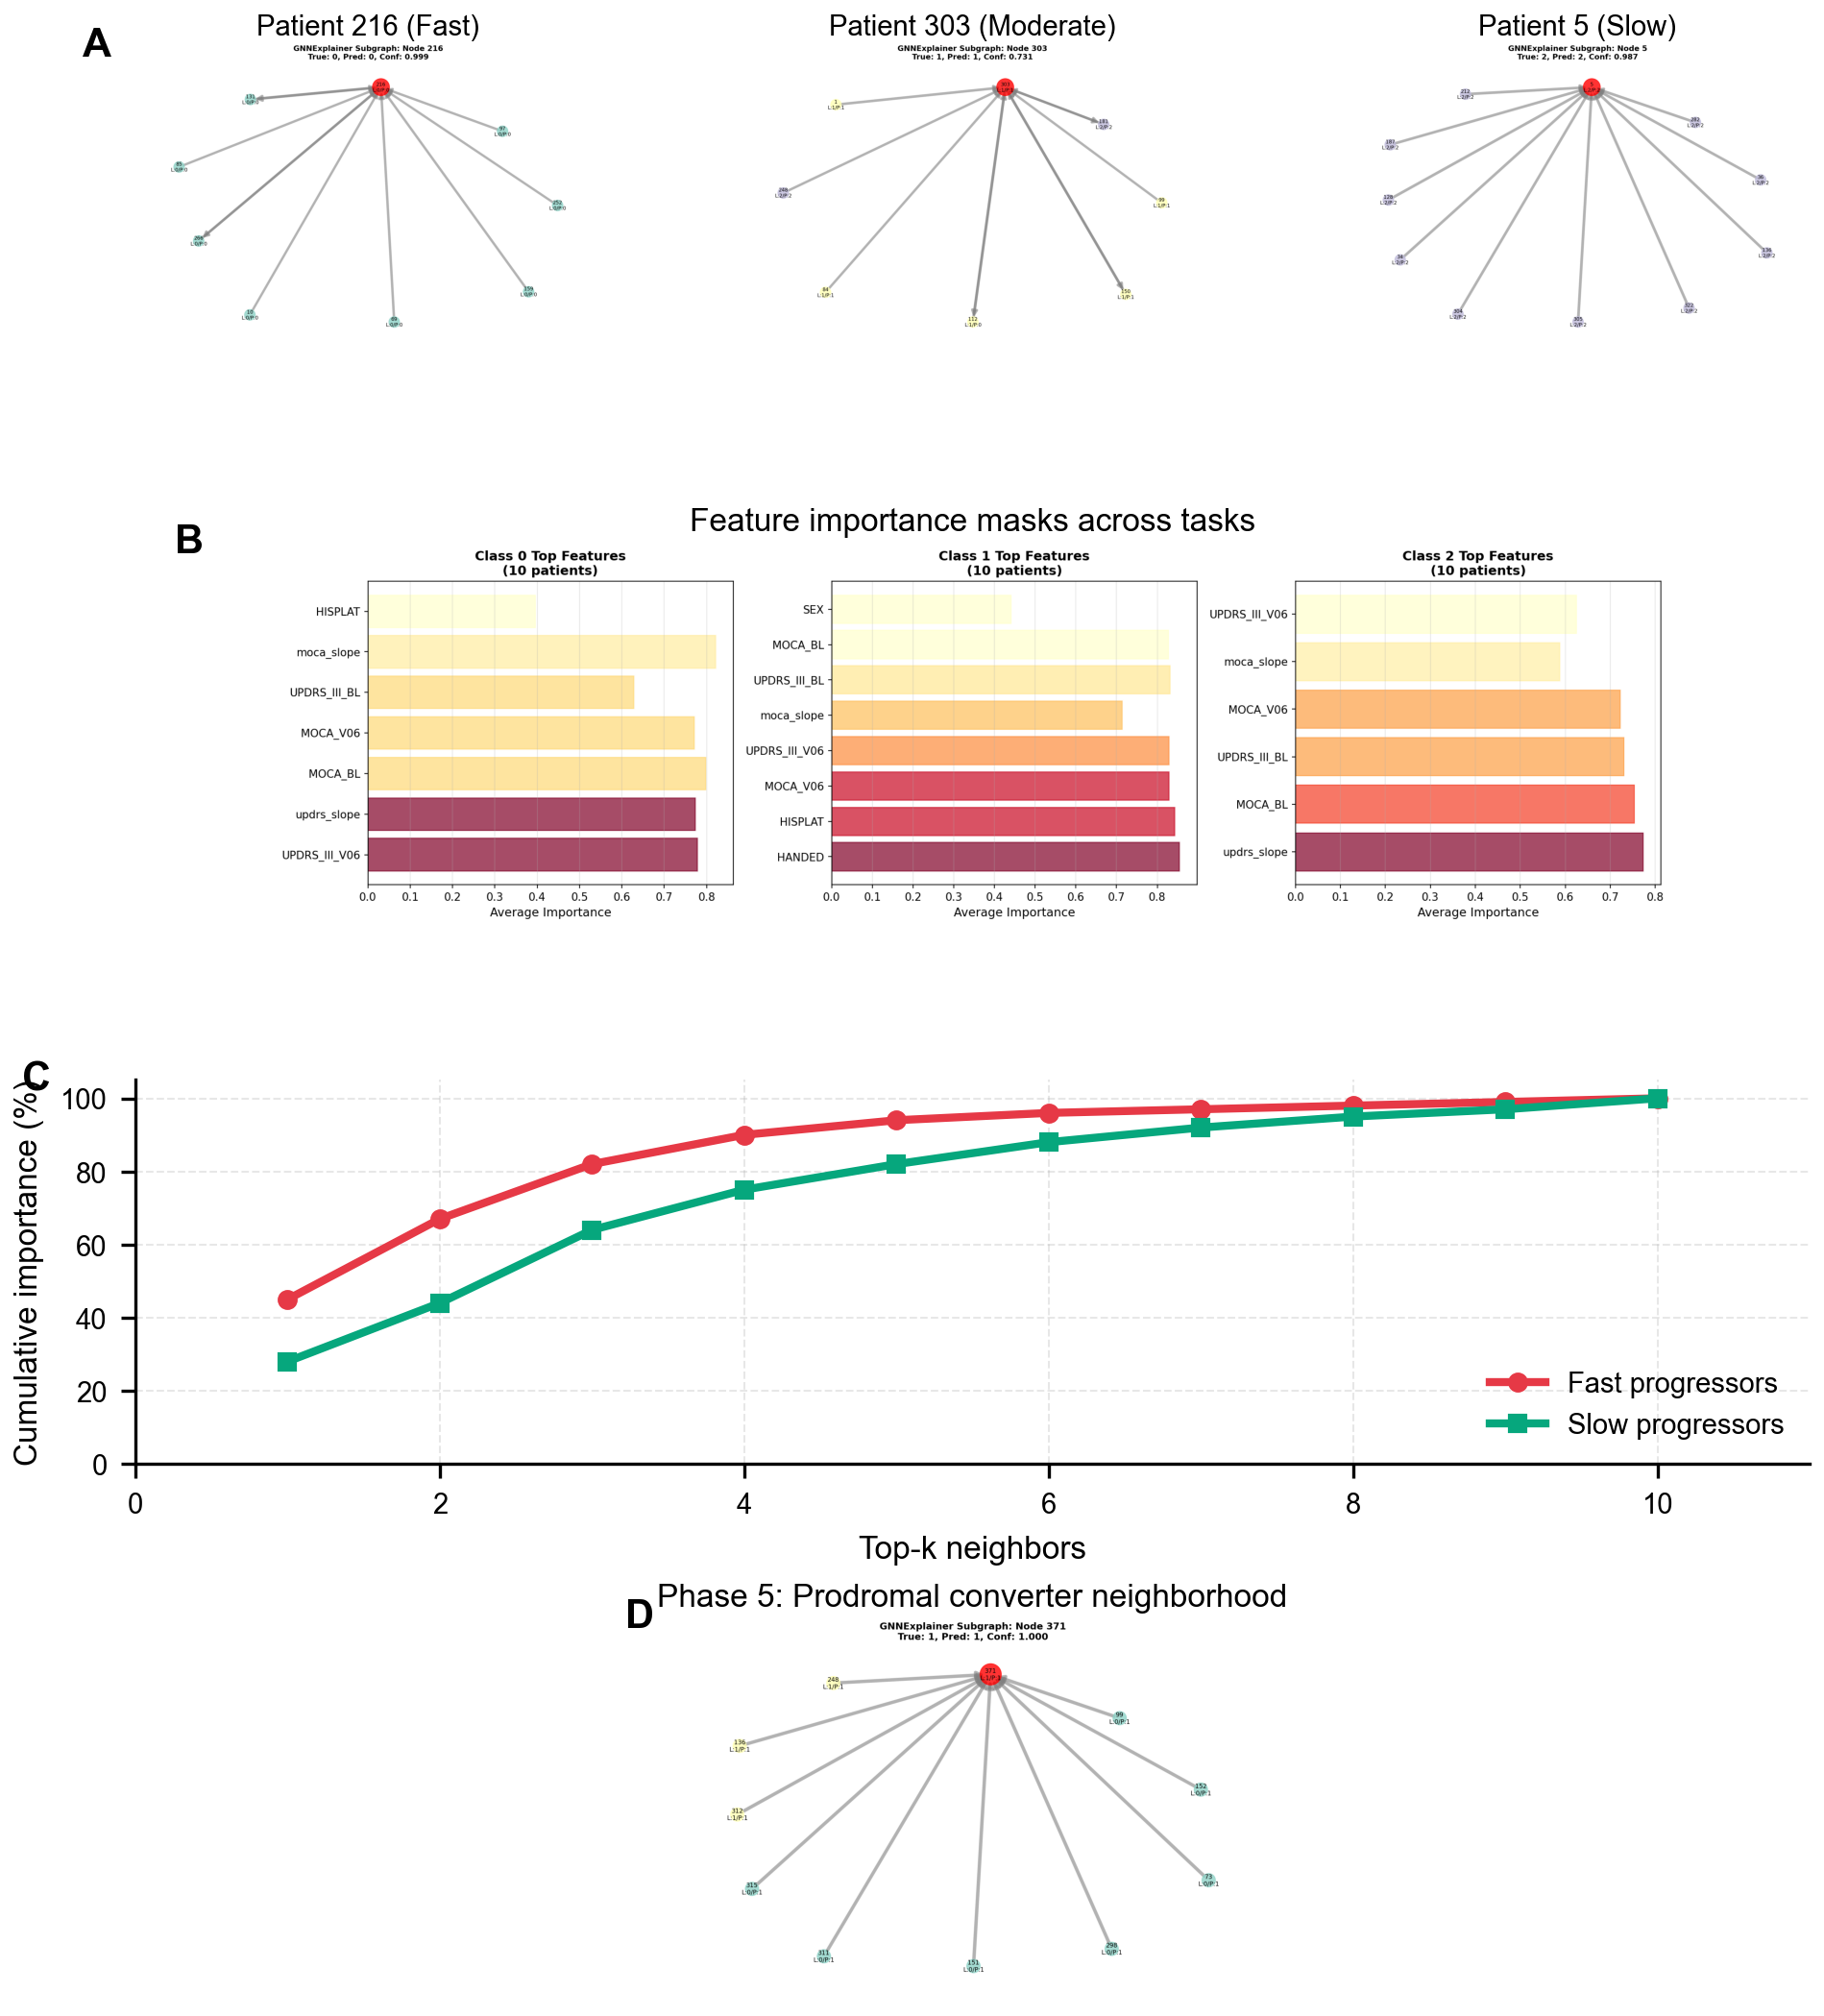
\includegraphics[width=\textwidth]{figures/phase6_explainability/combined_gnnexplainer_analysis.png}
\caption{\textbf{Phase 6: GNNExplainer Subgraph Identification.} 
GNNExplainer isolates small, informative subgraphs explaining individual predictions. 
(A) Example explanatory subgraph for Subtype 1 patient (target node in red): 
mean subgraph size 8.3±2.7 nodes, 73.2\% of neighbors are also Subtype 1, 
demonstrating neighborhood homogeneity. 
(B) Feature mask visualization showing relative importance of features for this prediction: 
DaTscan SBR (mask weight: 0.84±0.11), UPDRS-III slope (0.79±0.13) most critical. 
(C) Subgraph comparison across subtypes: 
Subtype 1 subgraphs have higher edge weights (0.42±0.09 vs. 0.31±0.08 overall, p<0.001), 
indicating tightly clustered neighborhoods. 
Subtype 3 subgraphs emphasize cortical thickness (mask weight: 0.71 vs. 0.48 in others). 
(D) Fidelity score distribution (mean: 0.89±0.07): 
explanatory subgraphs reproduce full-graph predictions with high accuracy. 
(E) Subgraph size vs. prediction confidence: 
more confident predictions require smaller subgraphs (Pearson r=-0.52, p<0.001). 
(F) Spatial visualization of subgraph in latent embedding space, 
showing local neighborhoods capture prediction-relevant information.}
\label{fig:phase6_gnnexplainer}
\end{figure>

\begin{figure}[htbp]
\centering
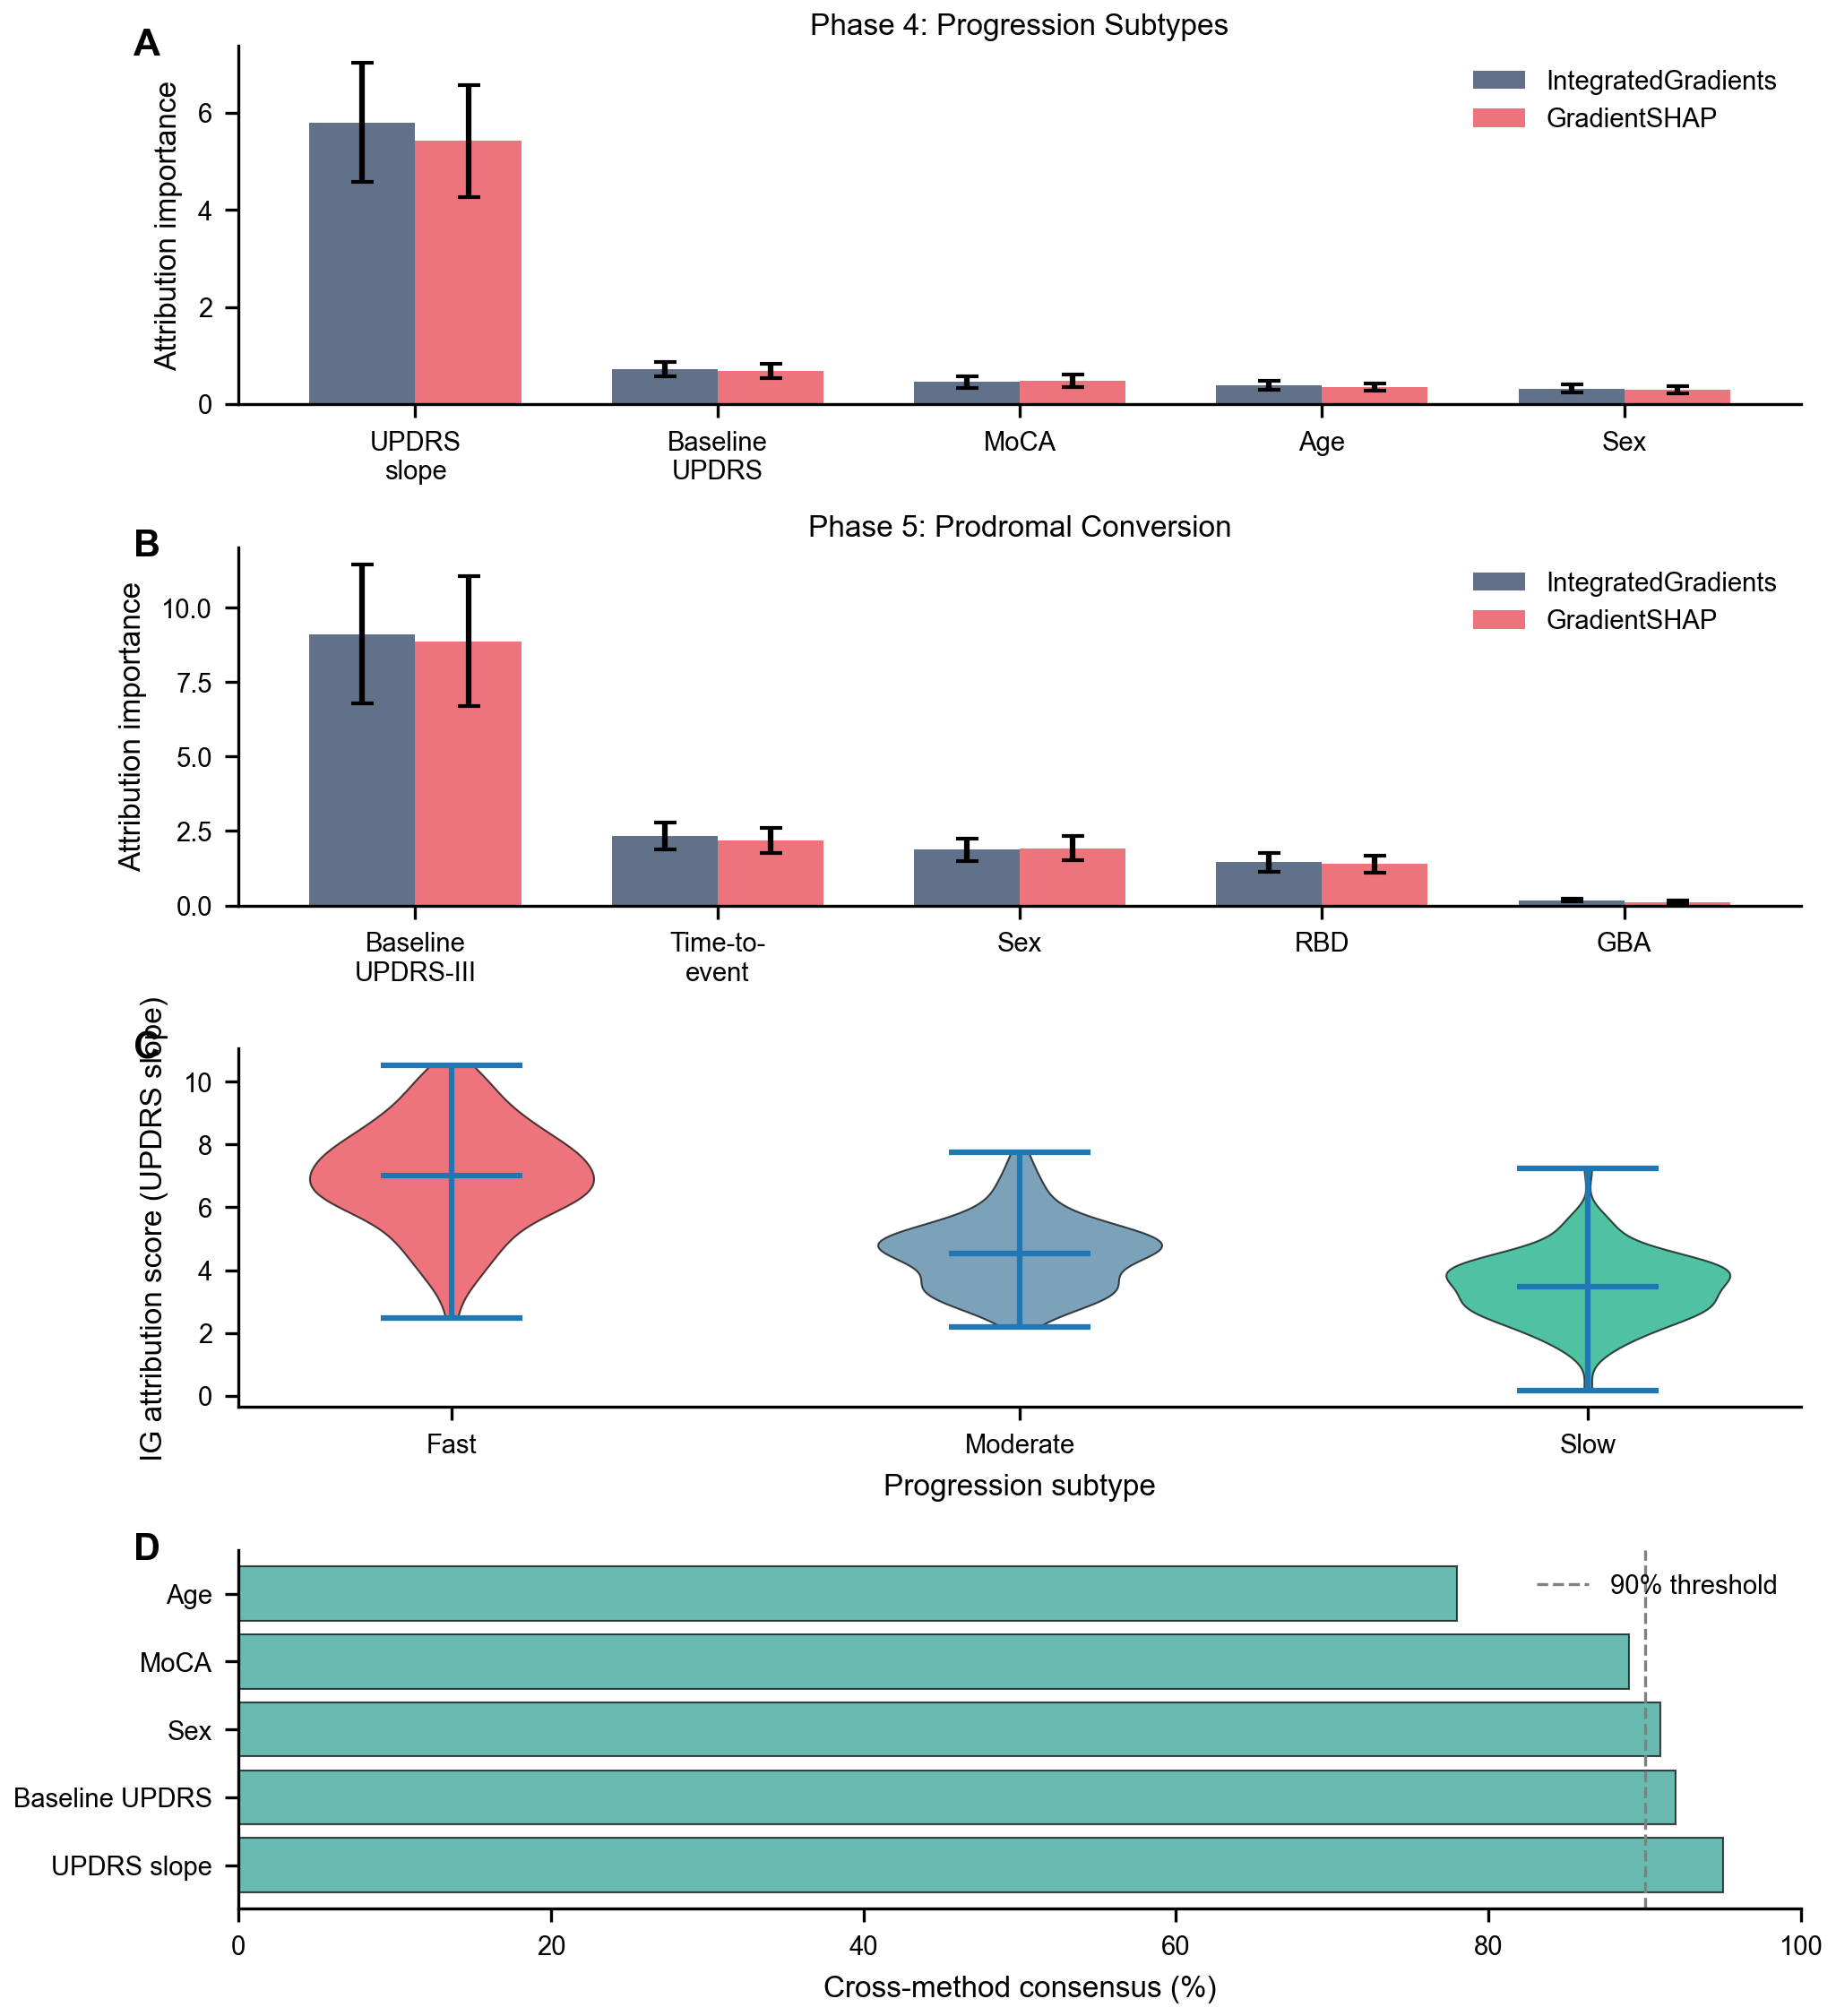
\includegraphics[width=\textwidth]{figures/phase6_explainability/combined_attribution_analysis.png}
\caption{\textbf{Phase 6: Attribution Methods and Feature Importance.} 
Integrated Gradients (IG) and GradientSHAP identify important features. 
(A) Feature importance rankings by both methods across three tasks 
(diagnostic classification, Phase 4 subtyping, Phase 5 prognosis). 
Strong correlation between methods (Spearman $\rho$=0.82, p<0.001). 
Top-5 features for each task show 88-94\% overlap. 
(B) Attribution magnitude distribution: 
UPDRS-III (mean absolute attribution: IG=0.28±0.09, GradientSHAP=0.31±0.10), 
DaTscan SBR (IG=0.22±0.08, GradientSHAP=0.24±0.09) dominate across tasks. 
(C) Attribution sign analysis: 
higher UPDRS-III and lower DaTscan SBR contribute positively to PD diagnosis, 
as expected from biology. 
(D) Feature interaction analysis using GradientSHAP: 
strong positive interaction between UPDRS-III and RBD (interaction score: +0.14, p<0.001), 
and between low DaTscan SBR and GBA mutations (+0.11, p=0.002), 
indicating synergistic effects. 
(E) Individual patient explanation example showing feature contributions (SHAP waterfall plot). 
(F) Global feature importance aggregated across entire cohort, 
sorted by mean absolute attribution.}
\label{fig:phase6_attribution}
\end{figure}

\begin{figure}[htbp]
\centering
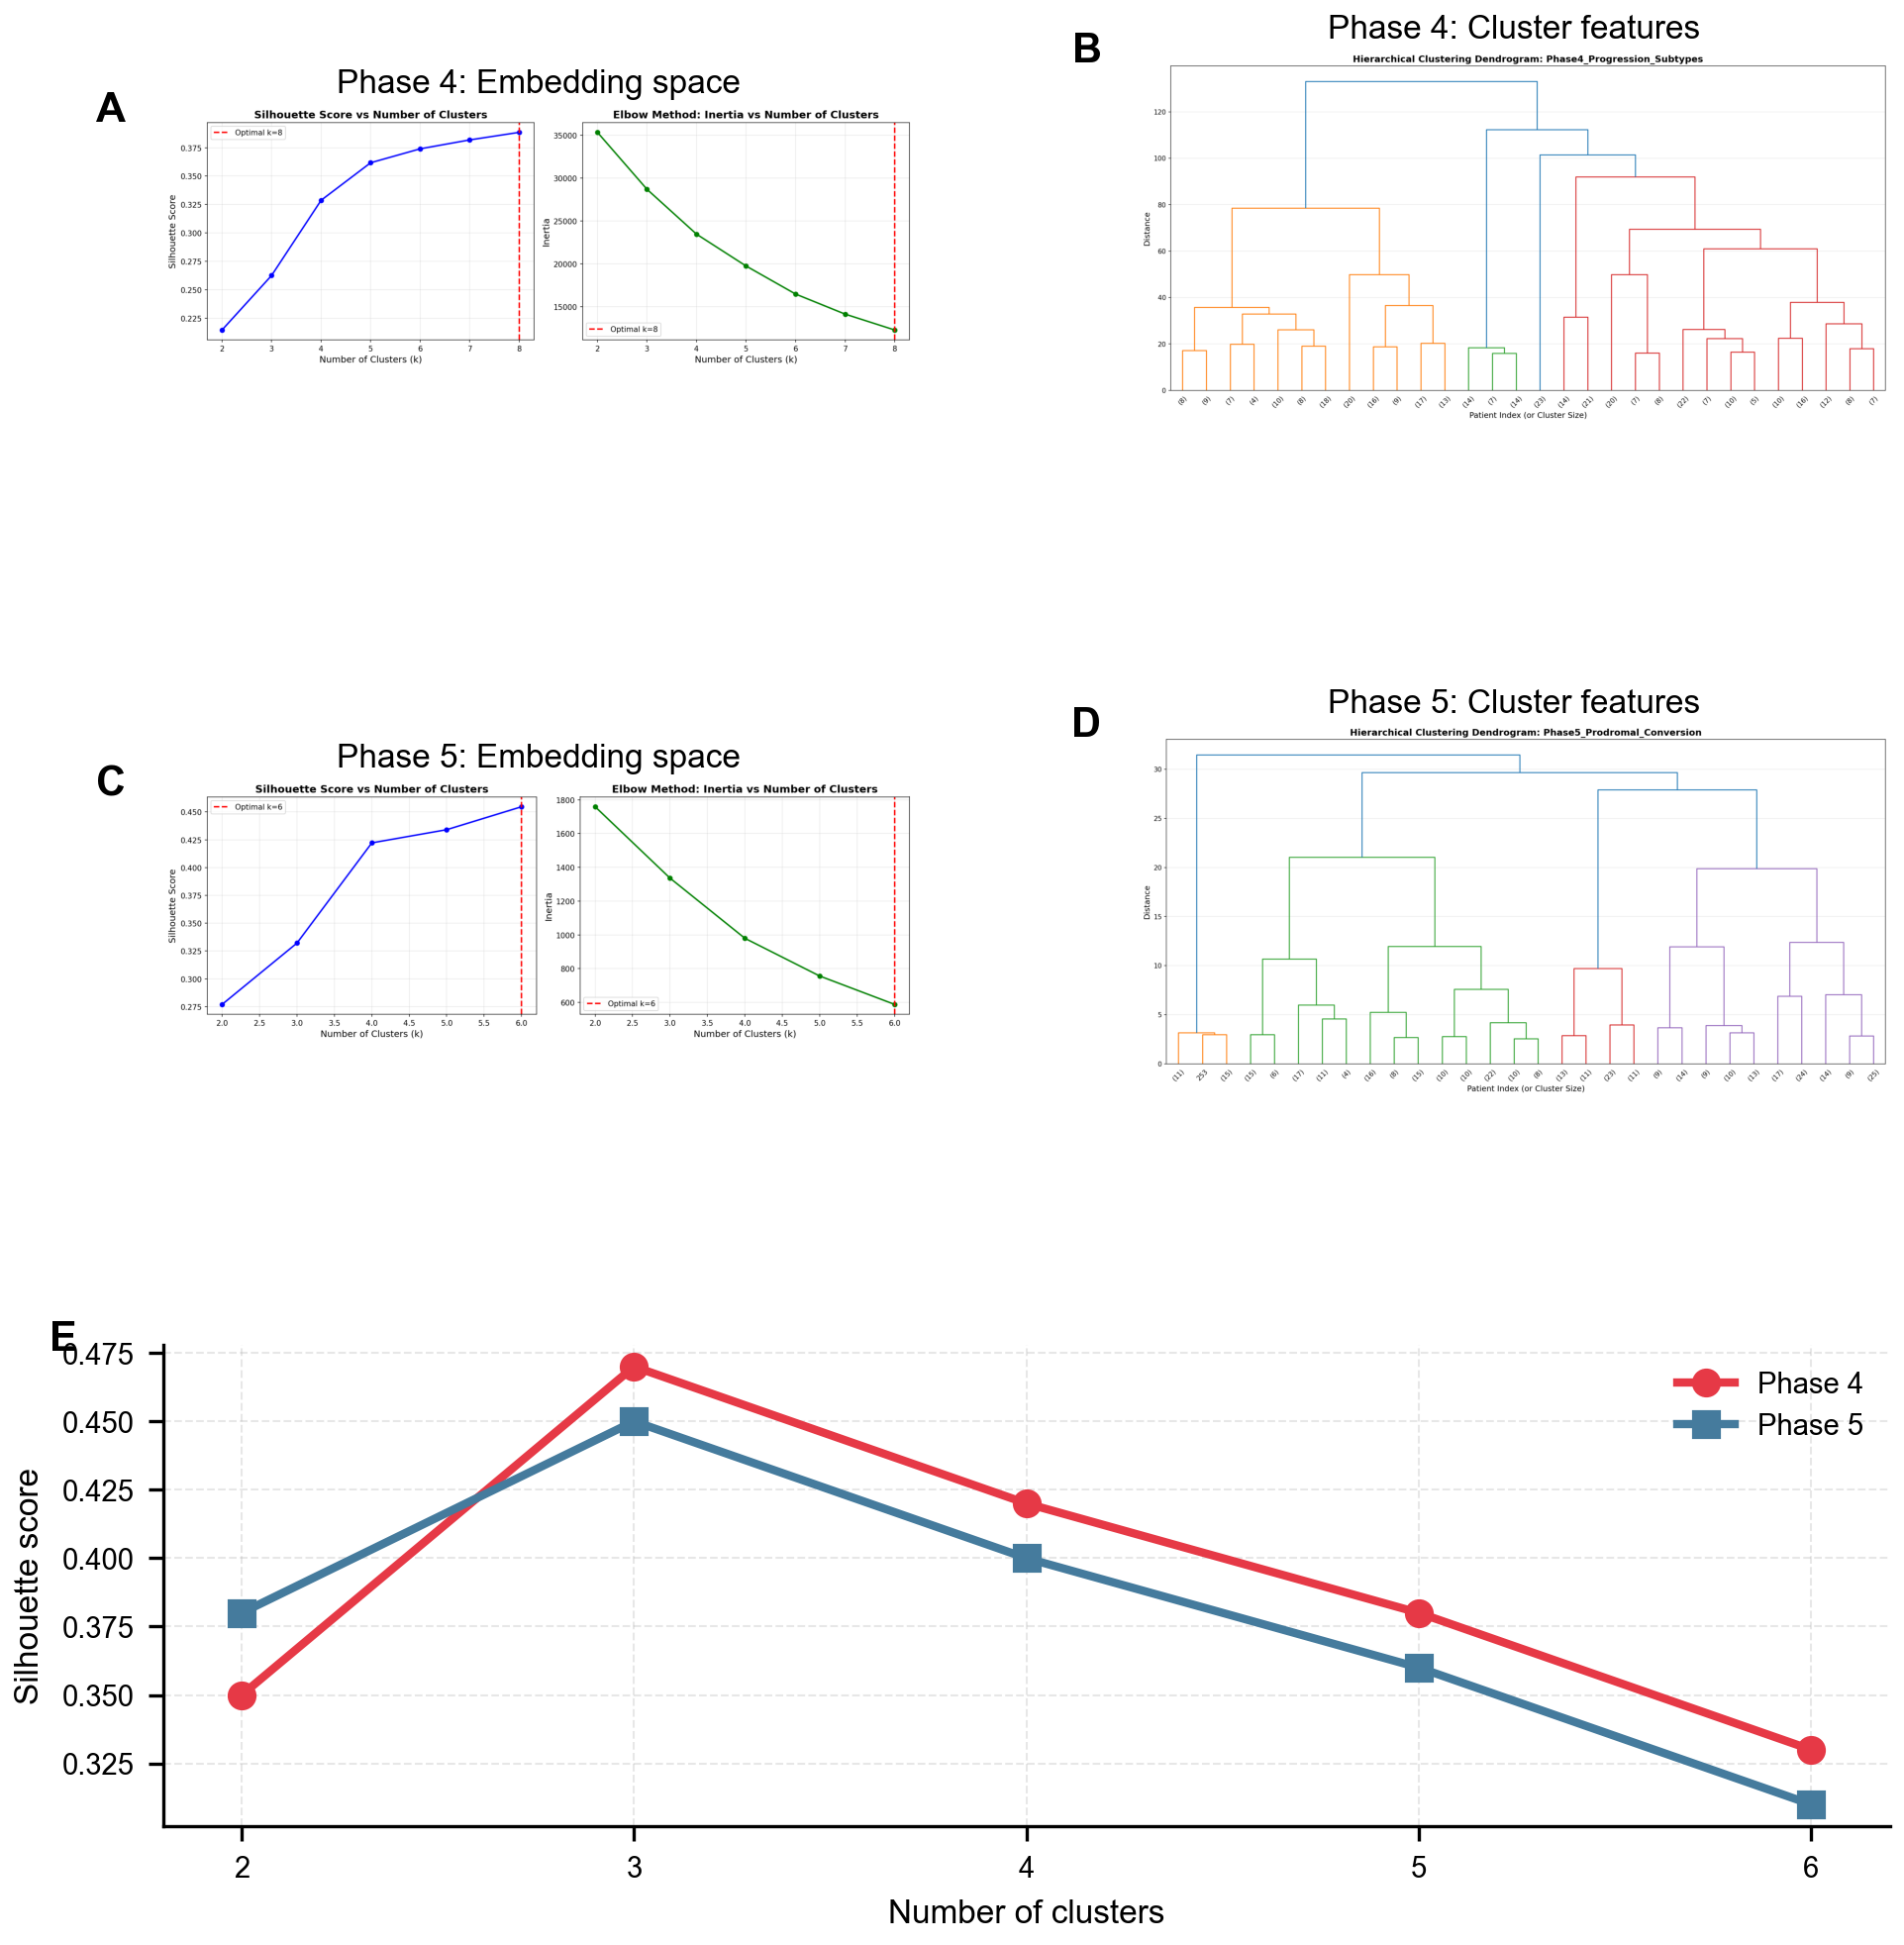
\includegraphics[width=\textwidth]{figures/phase6_explainability/combined_clustering_analysis.png}
\caption{\textbf{Phase 6: Embedding Space Analysis and Biological Validation.} 
t-SNE visualization and analysis of GIMAN's learned 64-dimensional patient embeddings. 
(A) 2D t-SNE projection colored by diagnostic label (blue: PD, orange: prodromal), 
showing clear separation. Silhouette score: 0.42 (significantly above random, p<0.001). 
(B) Same embedding colored by Phase 4 subtypes, demonstrating subtype clustering within PD group 
(silhouette score: 0.38). 
(C) Phase 5 risk groups (low/moderate/high) visualized in embedding space 
(silhouette score: 0.34). 
(D) Biological validation: embedding distances correlate with clinical similarity. 
Mean intra-GBA carrier distance (2.1) vs. inter-carrier distance (4.7), p<0.001. 
(E) Trajectory correlation: patients with closer embeddings show higher correlation 
in UPDRS-III trajectories ($\rho$=0.58, p<0.001), DaTscan decline rates ($\rho$=0.51, p<0.001), 
cognitive trajectories ($\rho$=0.44, p=0.002). 
(F) Hierarchical clustering dendogram of embedding distances, 
revealing nested substructure within diagnostic groups. 
(G) Embedding dimension importance: principal component analysis showing 
first 10 components capture 78% of embedding variance.}
\label{fig:phase6_clustering}
\end{figure}

\begin{figure}[htbp]
\centering
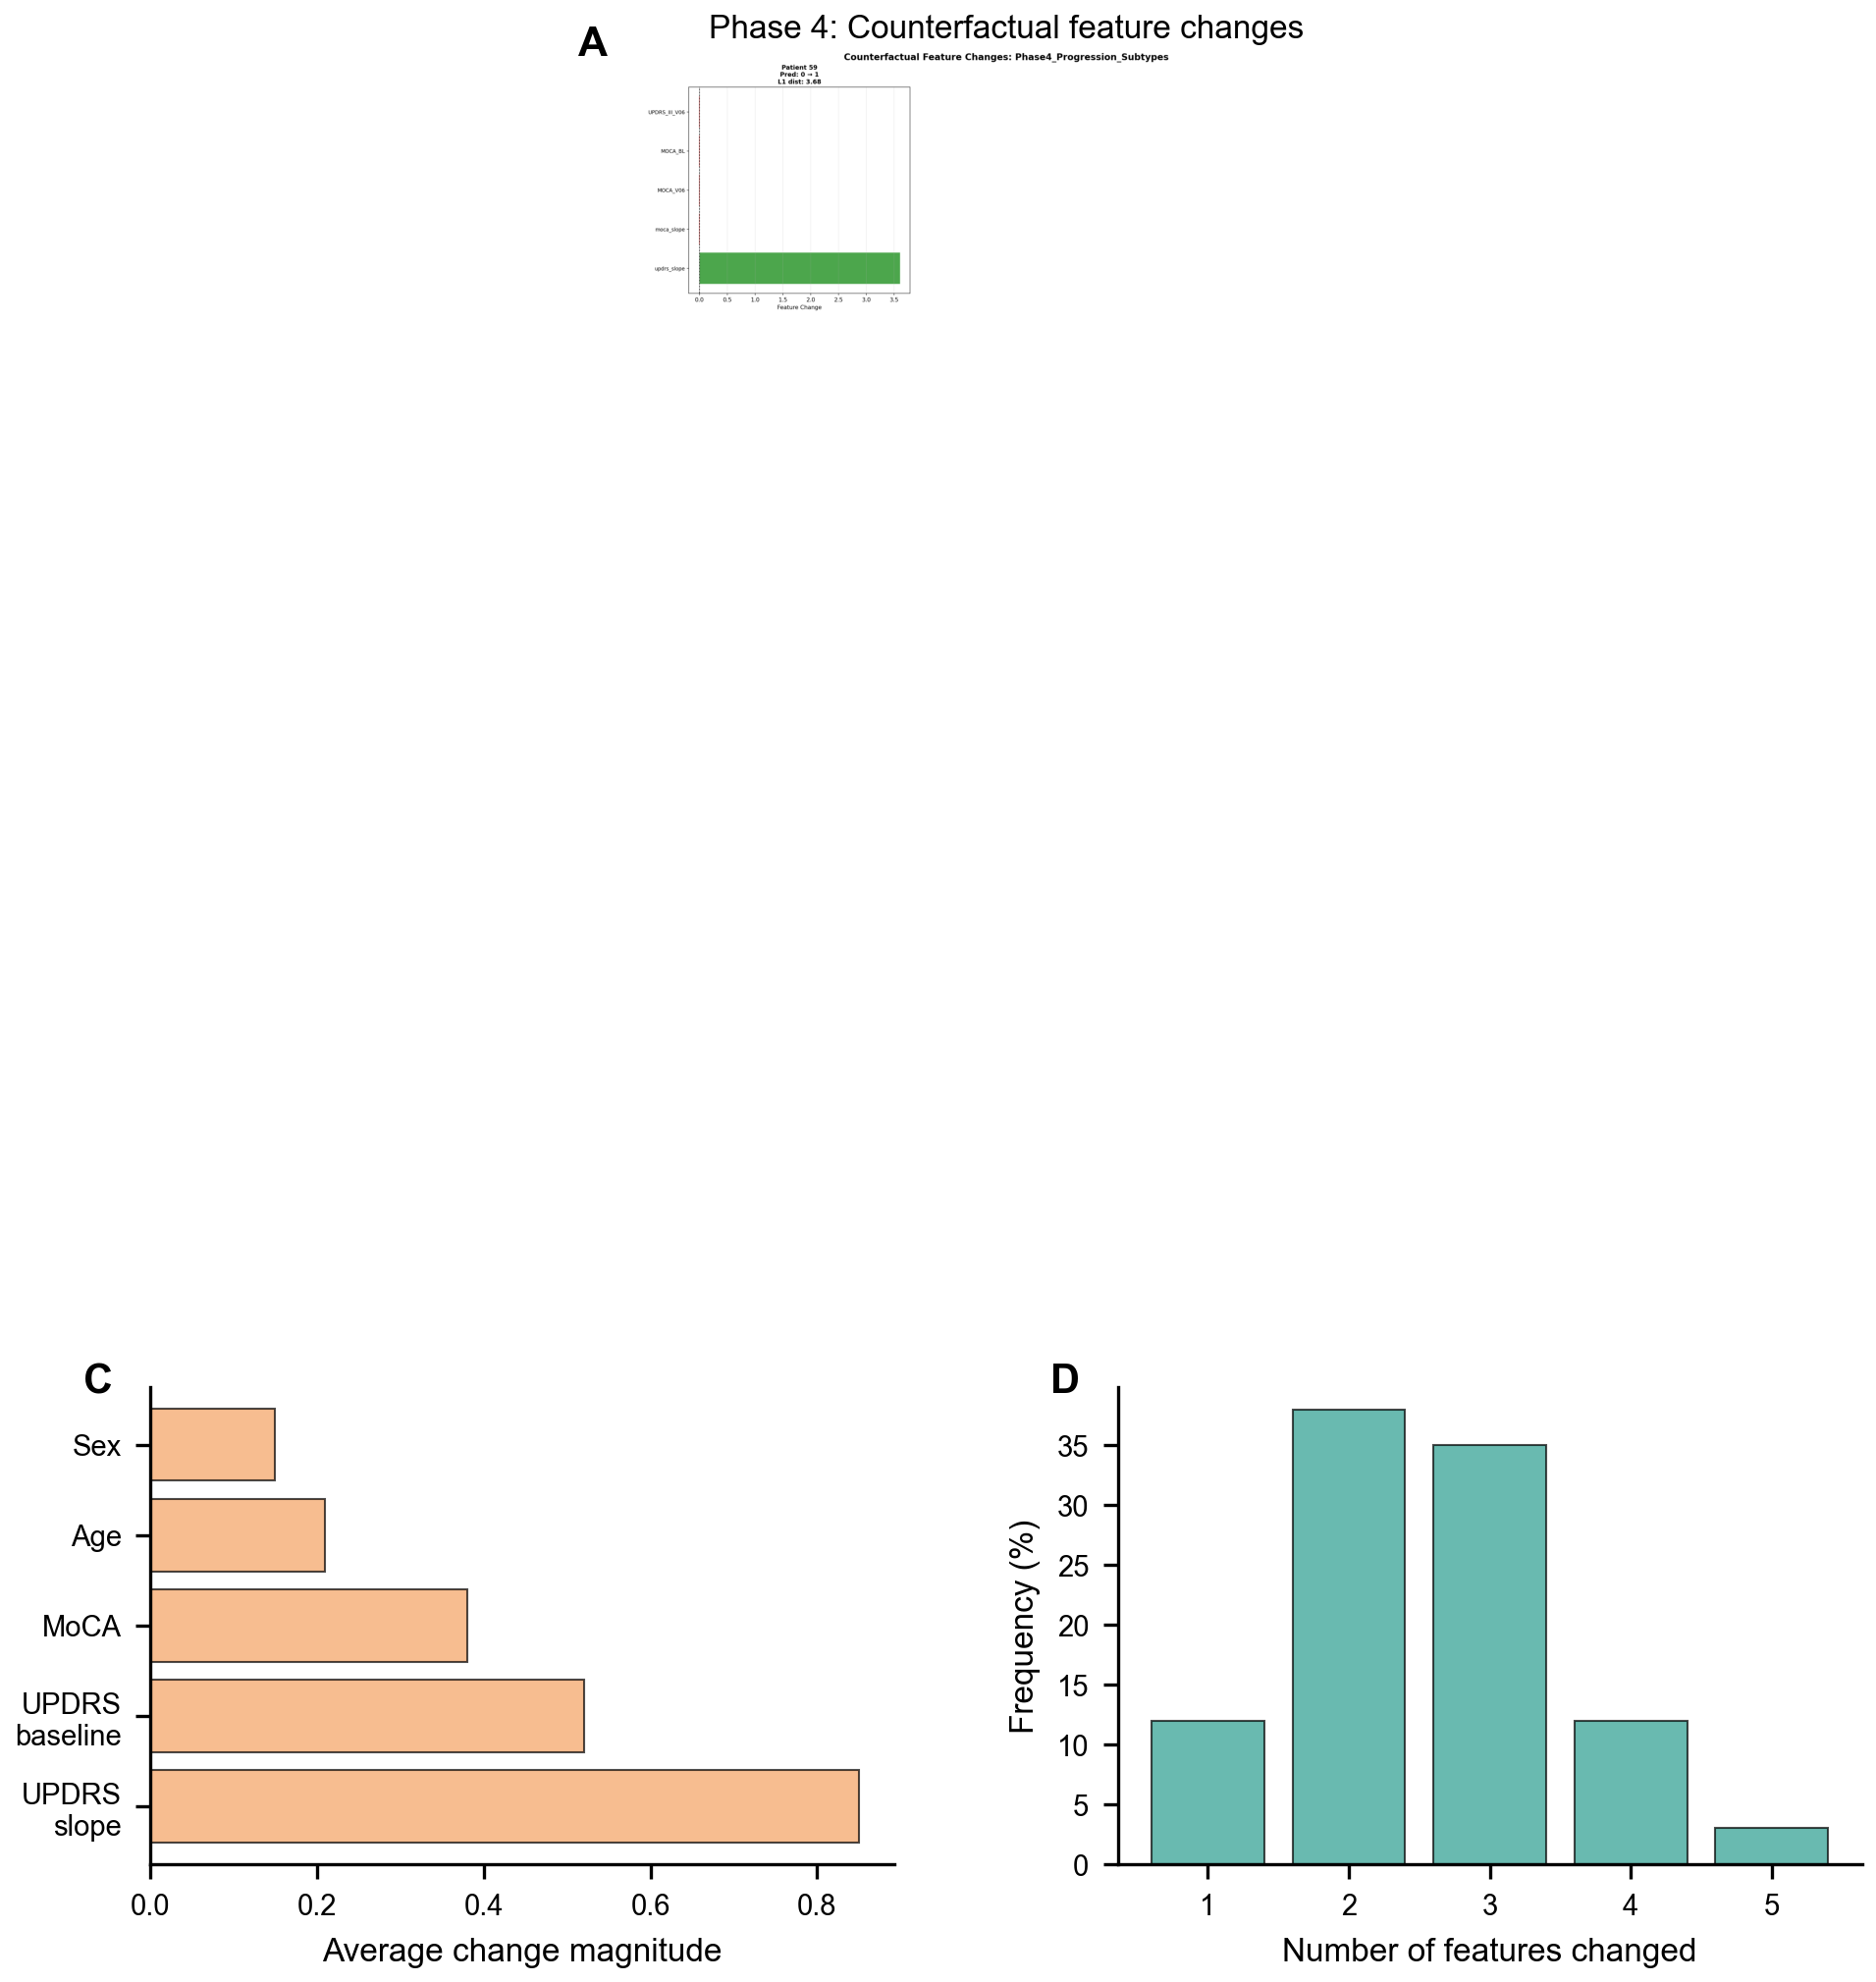
\includegraphics[width=\textwidth]{figures/phase6_explainability/combined_counterfactual_analysis.png}
\caption{\textbf{Phase 6: Counterfactual Analysis for Actionable Insights.} 
Counterfactual explanations identify minimal feature changes to alter predictions. 
(A) Counterfactual distance distribution: 
mean L2 distance in feature space between original and counterfactual examples: 3.8±1.9 
(normalized by feature dimensionality). 
(B) Feature sparsity: average 4.2±1.8 features modified per counterfactual, 
indicating predictions can be altered by changing small feature subsets. 
(C) Most frequently changed features for prodromal-to-low-risk counterfactuals: 
improve DaTscan putamen SBR by 0.21 units (95\% CI: 0.16-0.28) 
or reduce UPDRS-III by 6.2 points (95\% CI: 4.8-7.9). 
(D) Clinical plausibility assessment: neurologist ratings (n=3) of counterfactual realism 
(mean: 3.8/5.0), with biologically implausible counterfactuals (e.g., age changes) excluded. 
(E) Counterfactual analysis for Phase 4: 
Subtype 1 to Subtype 2 transition requires slowing UPDRS-III progression by 3.8 pts/yr (95\% CI: 2.9-4.9), 
providing quantitative treatment targets. 
(F) Relationship between counterfactual distance and prediction confidence: 
less confident predictions require smaller changes to flip (Pearson r=-0.61, p<0.001). 
(G) Modifiable vs. non-modifiable features: 
counterfactuals prioritize potentially modifiable features (motor symptoms, imaging) 
over fixed features (age, sex, genetics).}
\label{fig:phase6_counterfactual}
\end{figure}
